\chapter{Controller Test Results}\label{app:controllerTestResults}
\todo[inline]{Fix figures with sim results.}
\begin{figure}[tbp]
  \centering
  \subfloat[][\label{fig:ApptestStepRoll} A smooth step applied in $\rollAngle$.]{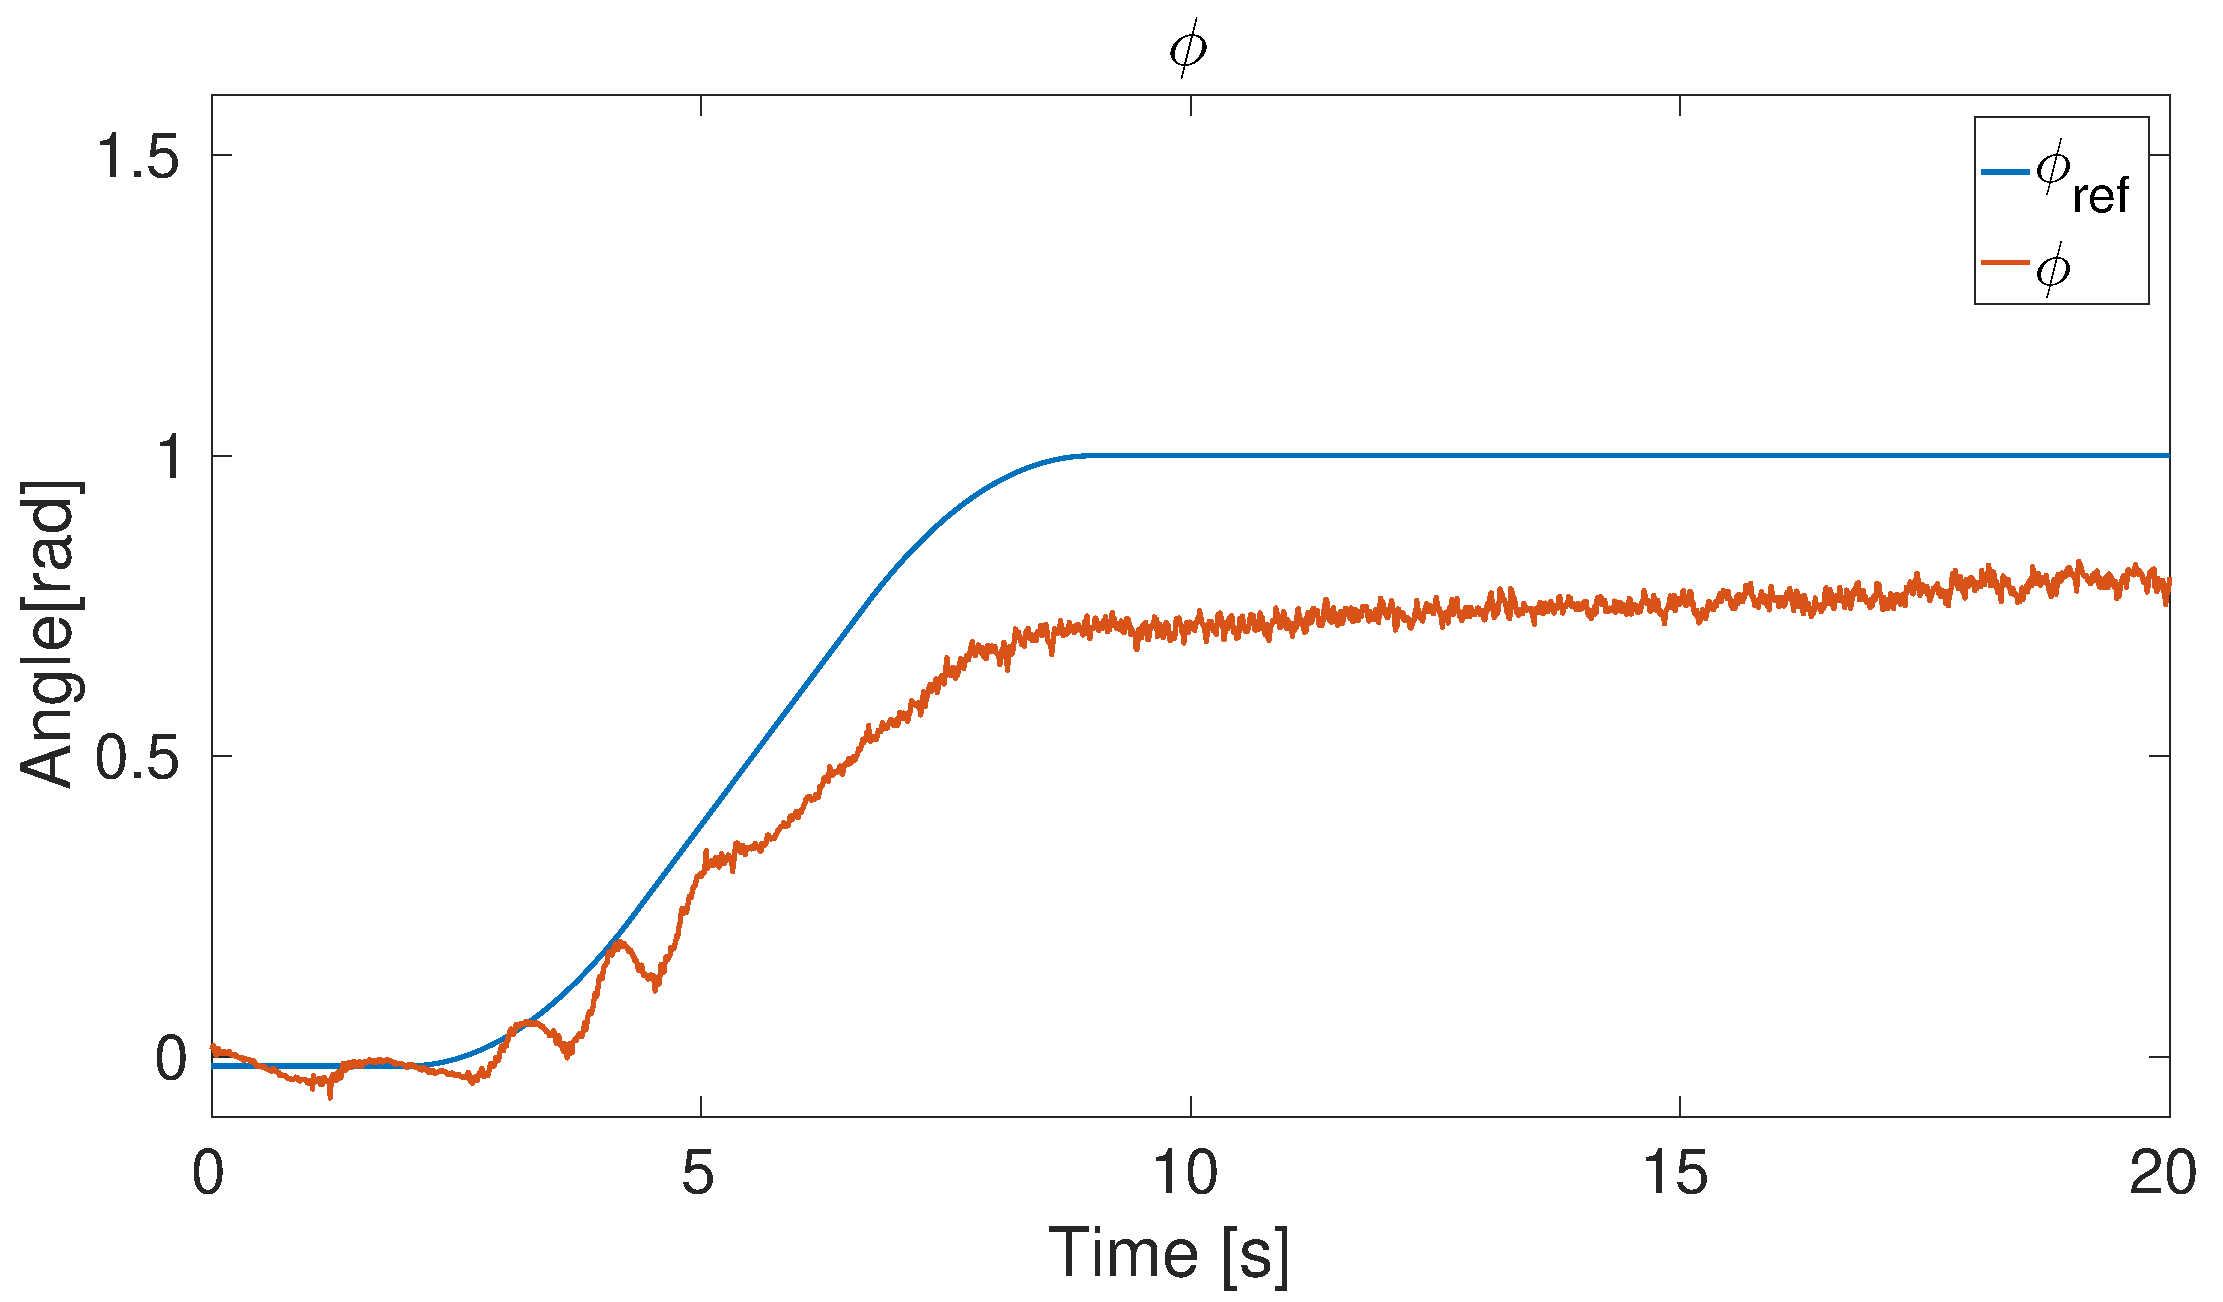
\includegraphics[width=0.4\textwidth]{testStepPhis3e10a1}}
  \qquad
  \subfloat[][\label{fig:AppsimStepRoll} A step applied to the simulated \abbrROV in $\rollAngle$.]{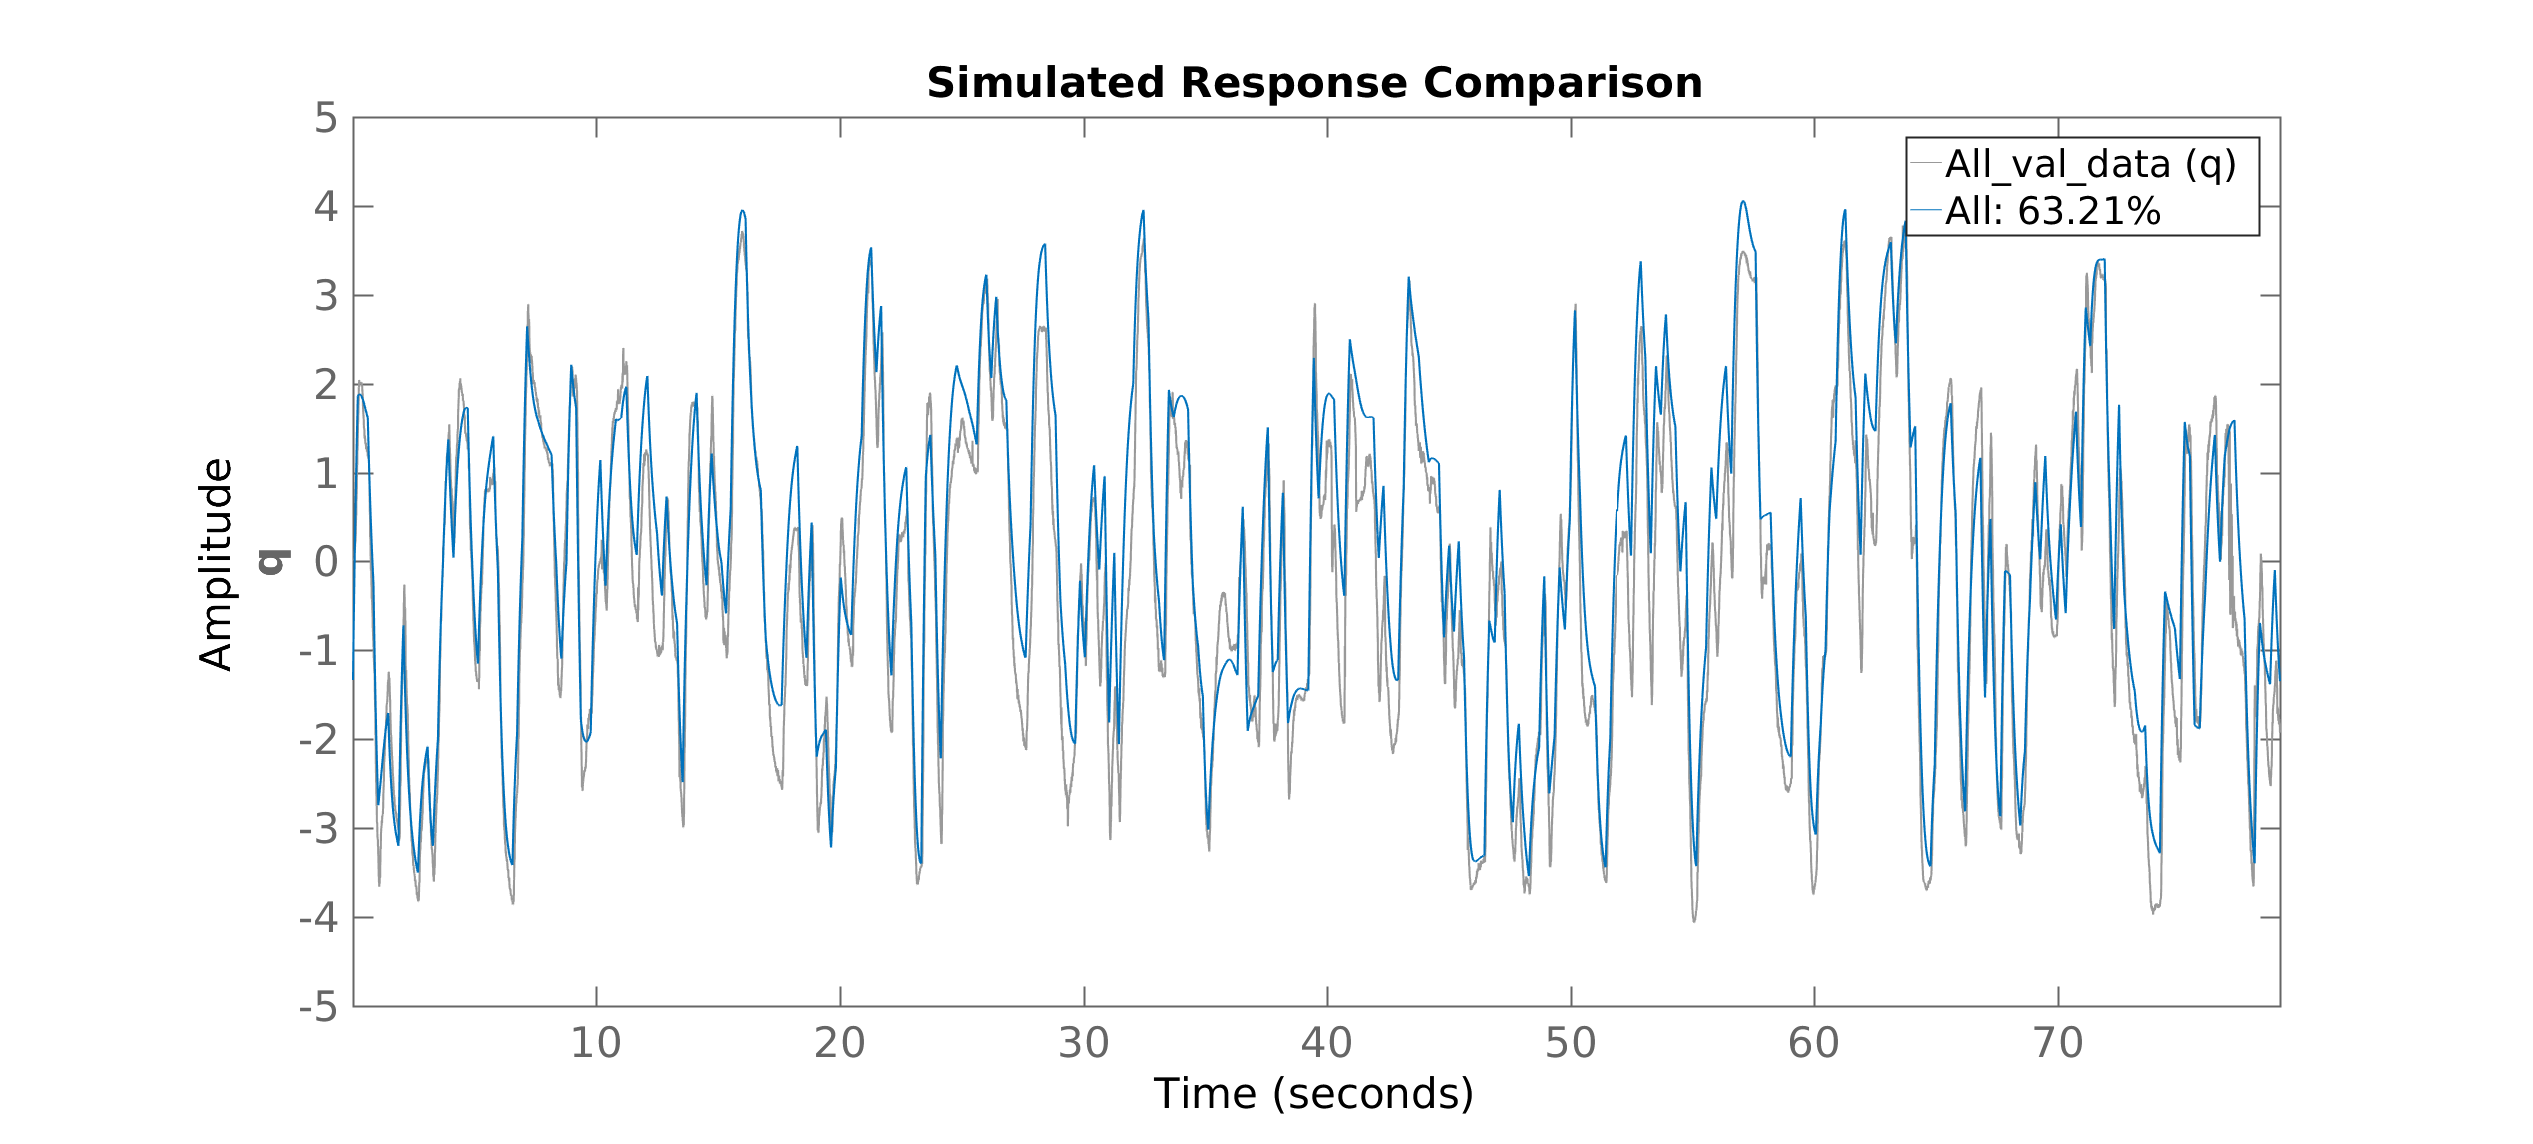
\includegraphics[width=0.4\textwidth]{velocityCompareq}}
  \qquad
  \subfloat[][\label{fig:ApptestStepPitch} A smooth step applied in $\pitchAngle$.]{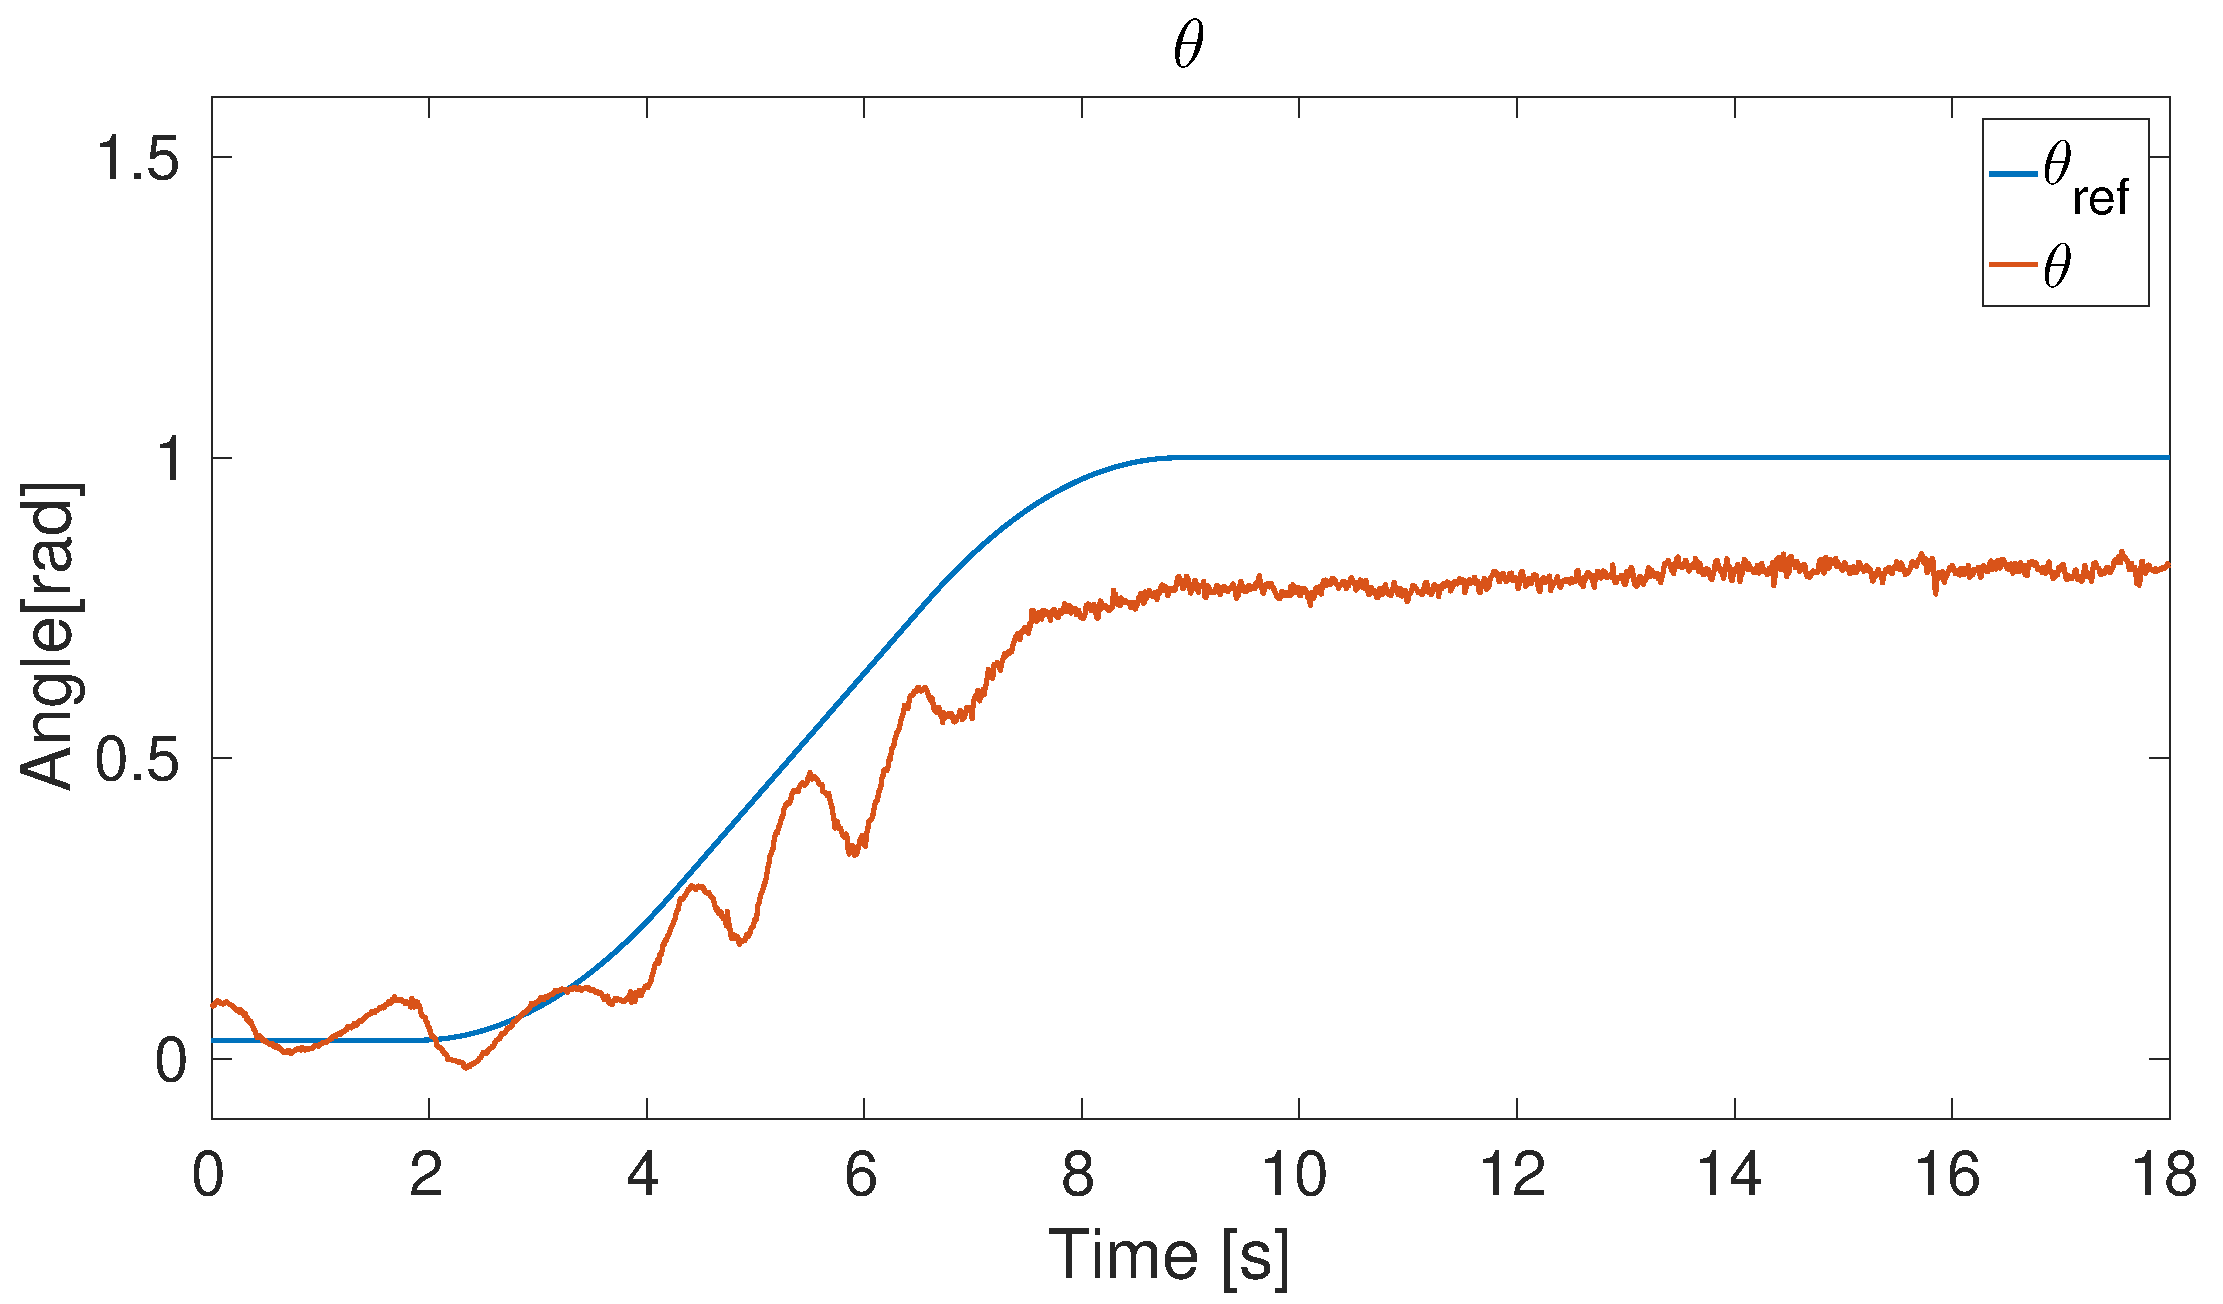
\includegraphics[width=0.4\textwidth]{testStepThetas3e10a1}}
  \qquad
  \subfloat[][\label{fig:AppsimStepPitch} A smooth step applied to the simulated \abbrROV in $\pitchAngle$.]{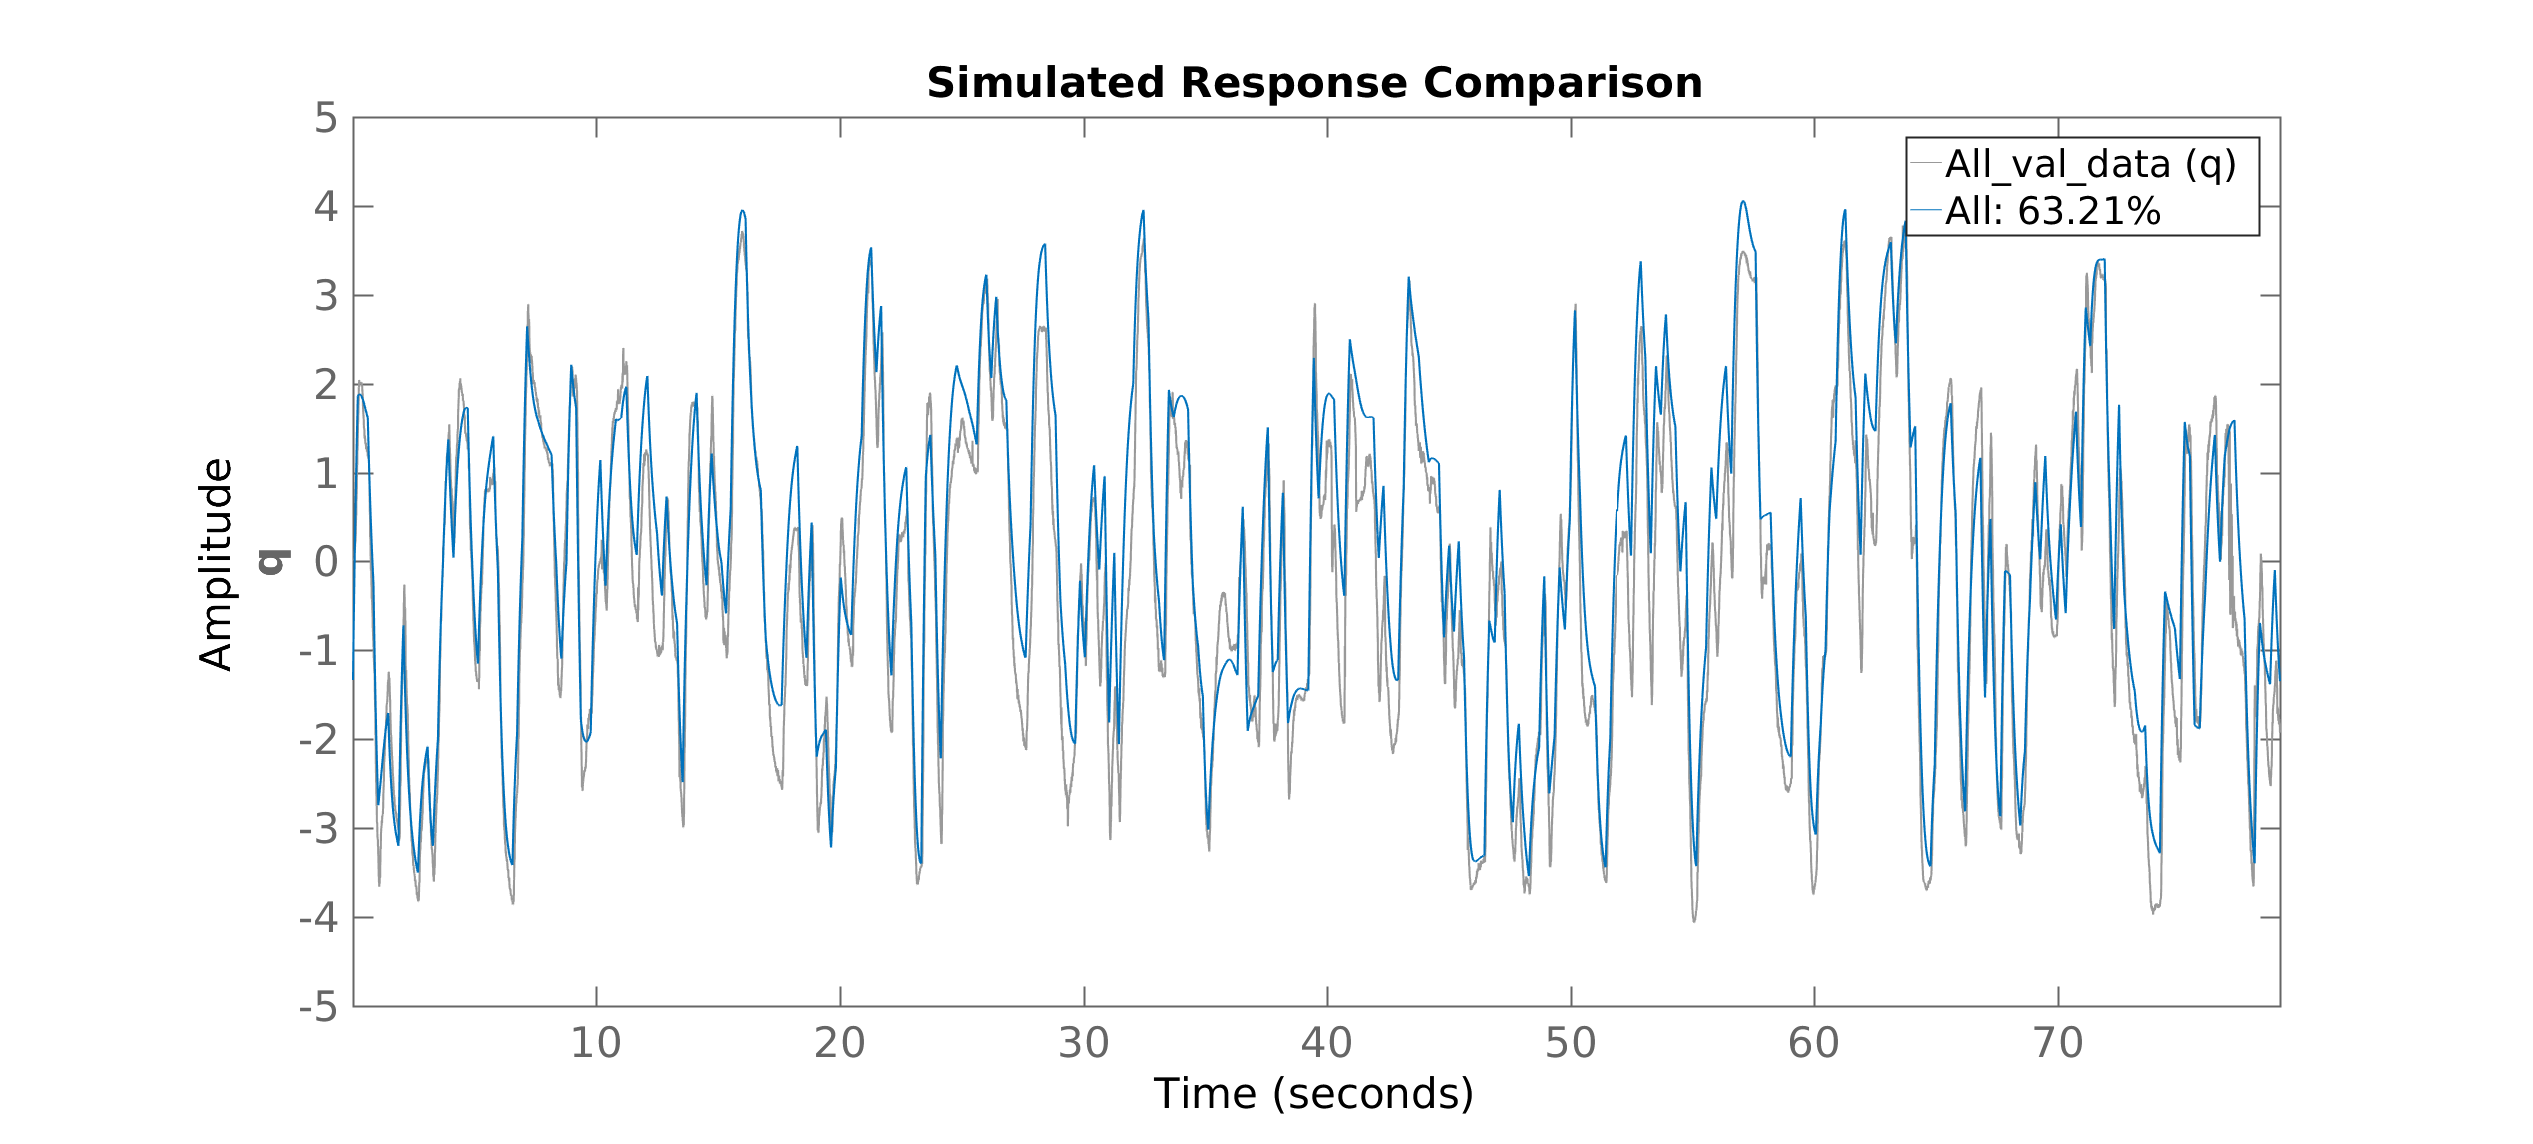
\includegraphics[width=0.4\textwidth]{velocityCompareq}}
  \qquad
  \subfloat[][\label{fig:ApptestStepYaw} A smooth step applied in $\yawAngle$.]{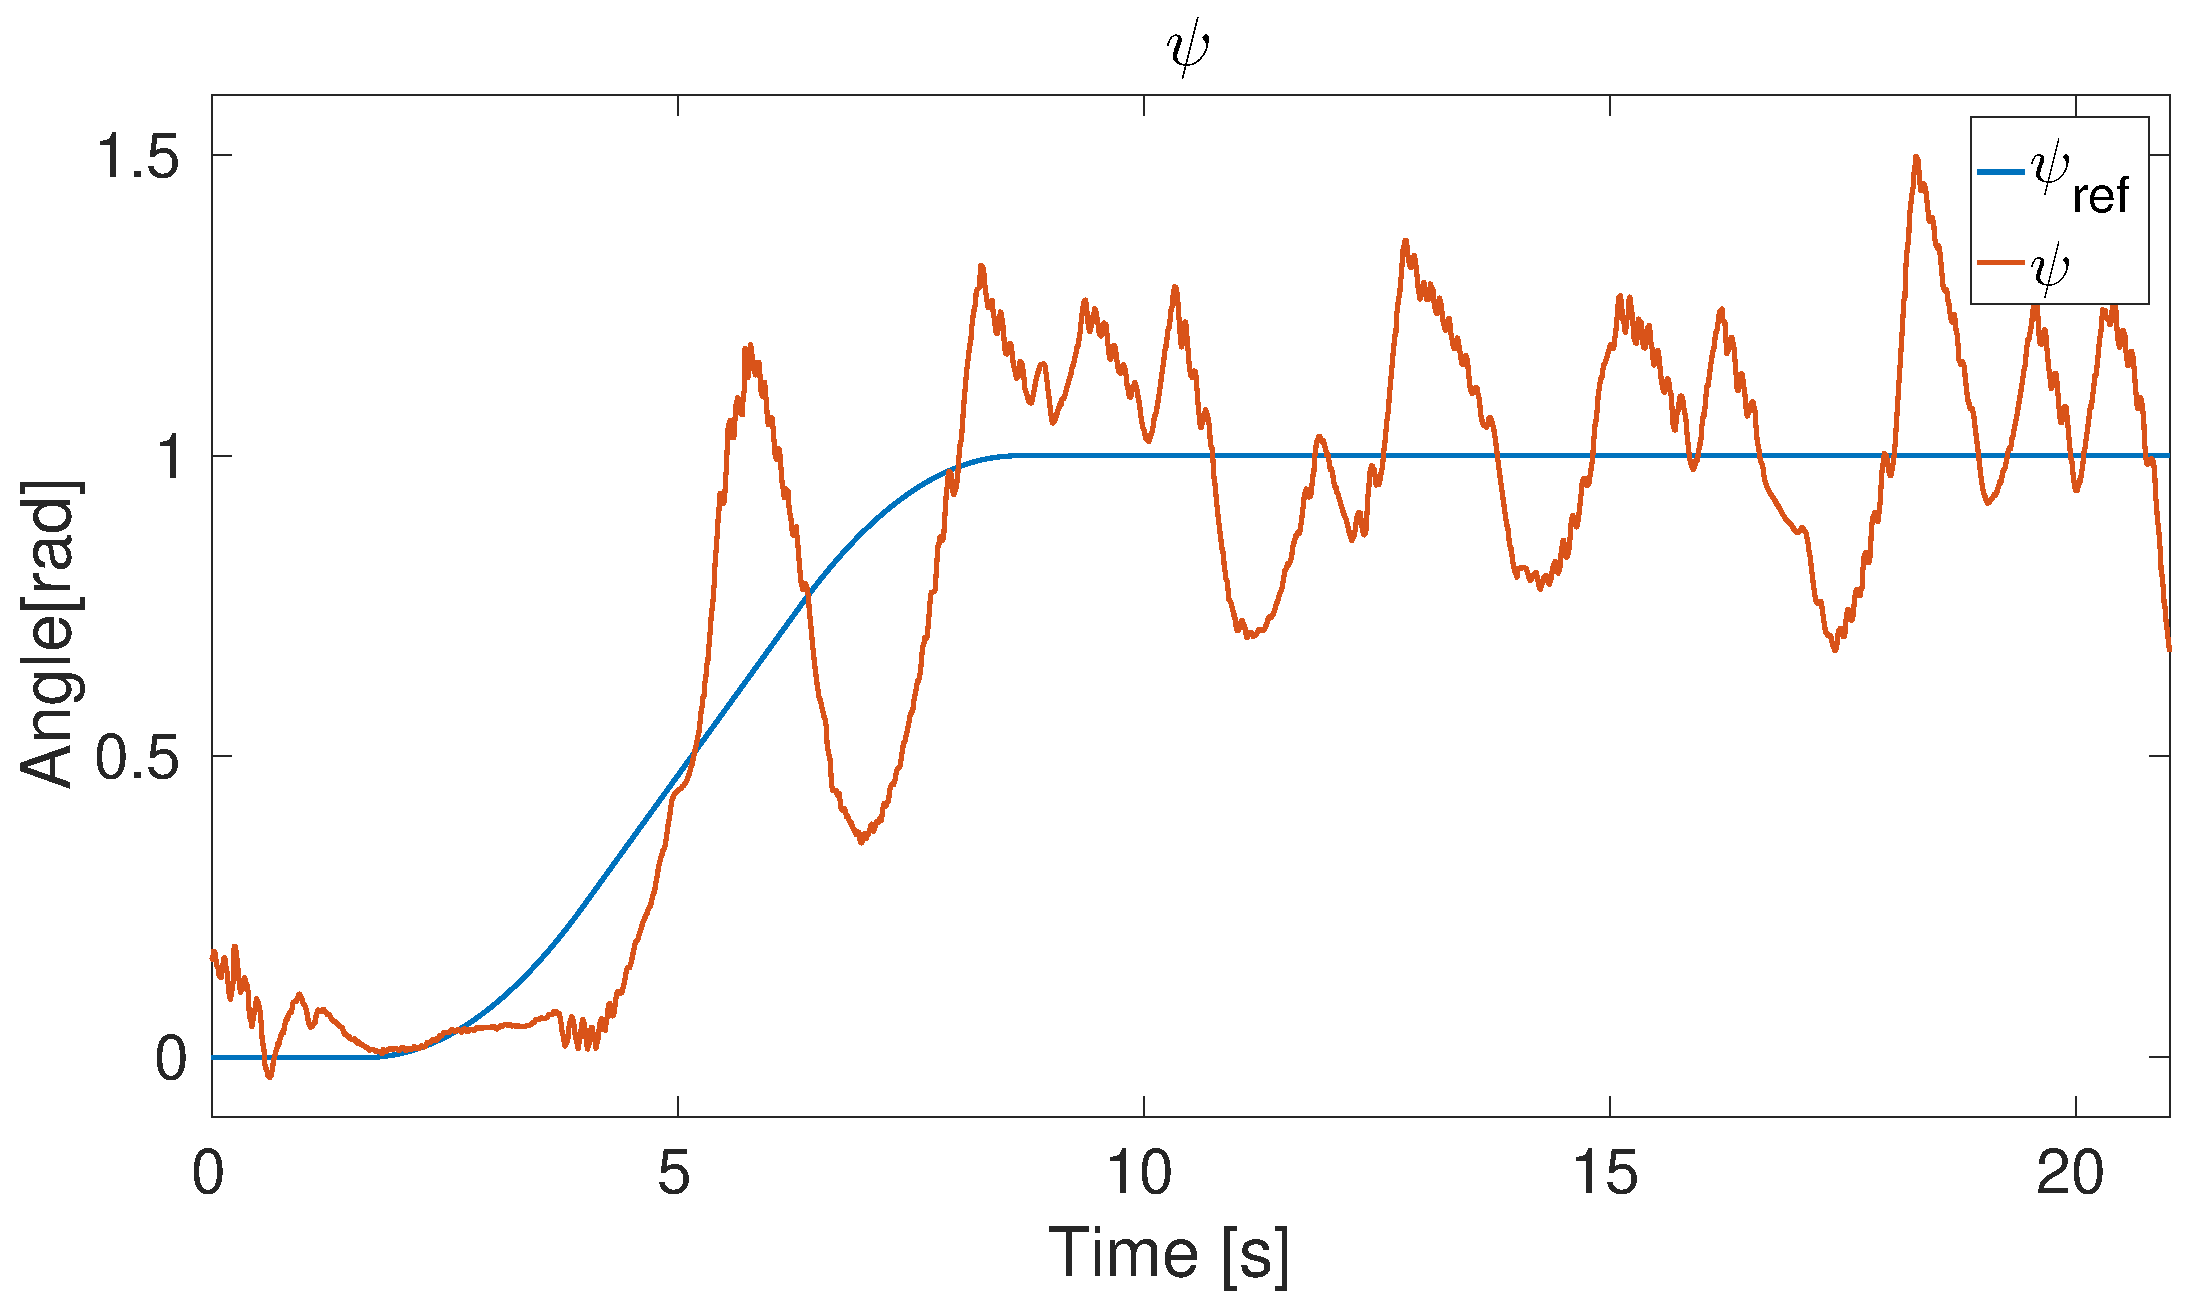
\includegraphics[width=0.4\textwidth]{testStepPsis3e10a1}}
  \qquad
  \subfloat[][\label{fig:AppsimStepYaw} A smooth step applied to the simulated \abbrROV in $\yawAngle$.]{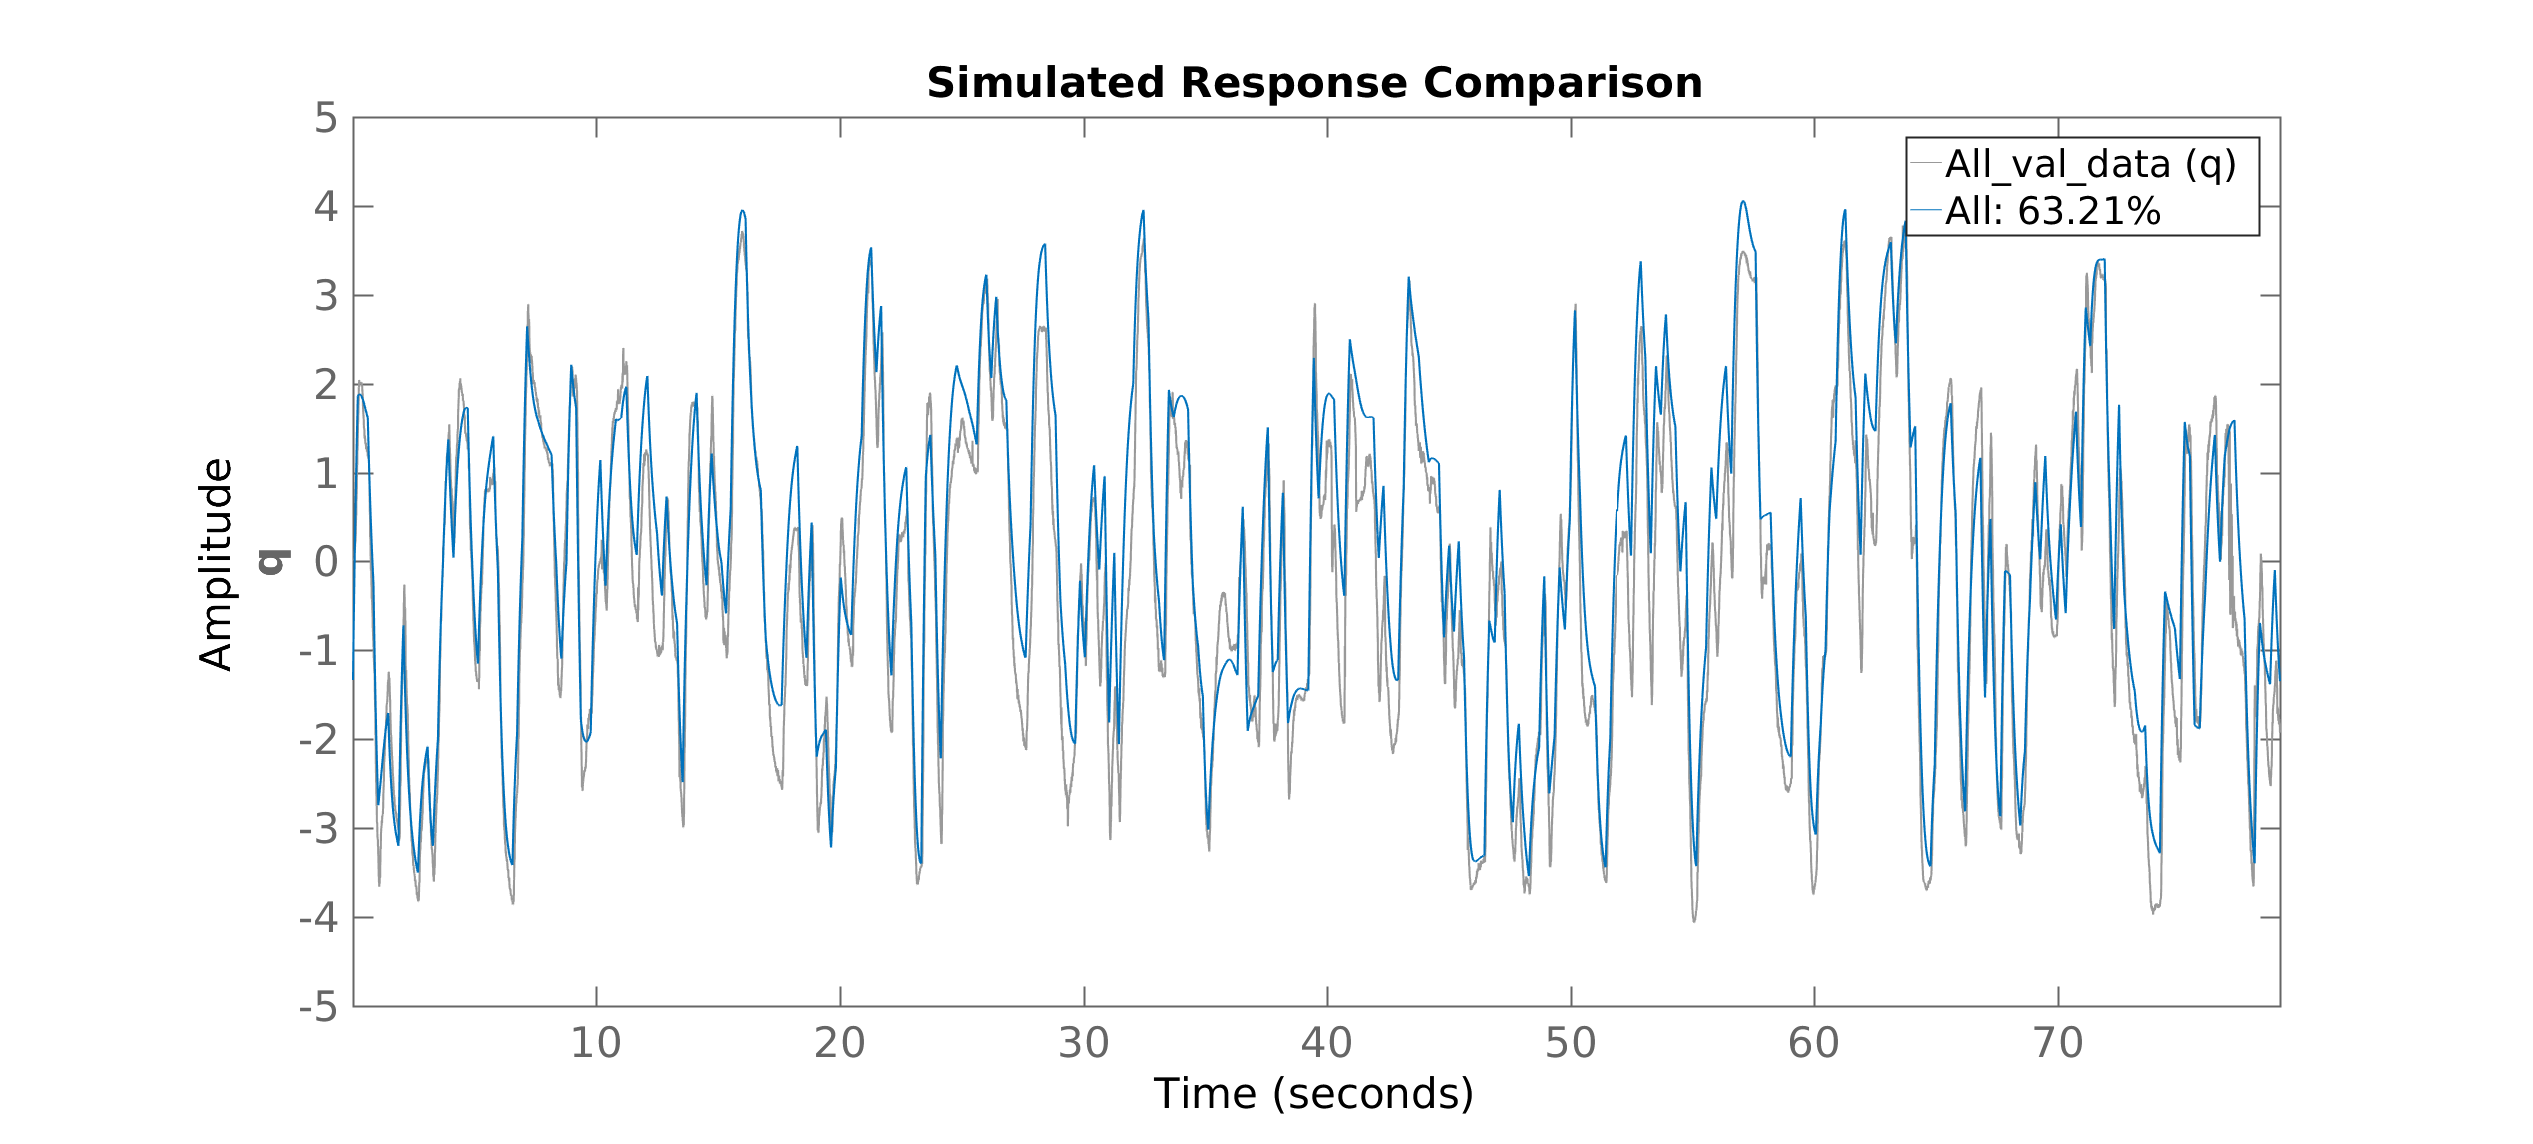
\includegraphics[width=0.4\textwidth]{velocityCompareq}}
   \caption{\label{fig:AppStepAttitude}%
   A smooth step was applied in one attitude angle at a time while using the attitude controller. While a smooth step was applied in one attitude angle the other attitude angles were not controlled.}
\end{figure}

\begin{figure}
\centering
  \subfloat[][\label{fig:ApptestStepAllRollAttitude} A smooth step applied in $\rollAngle$.]{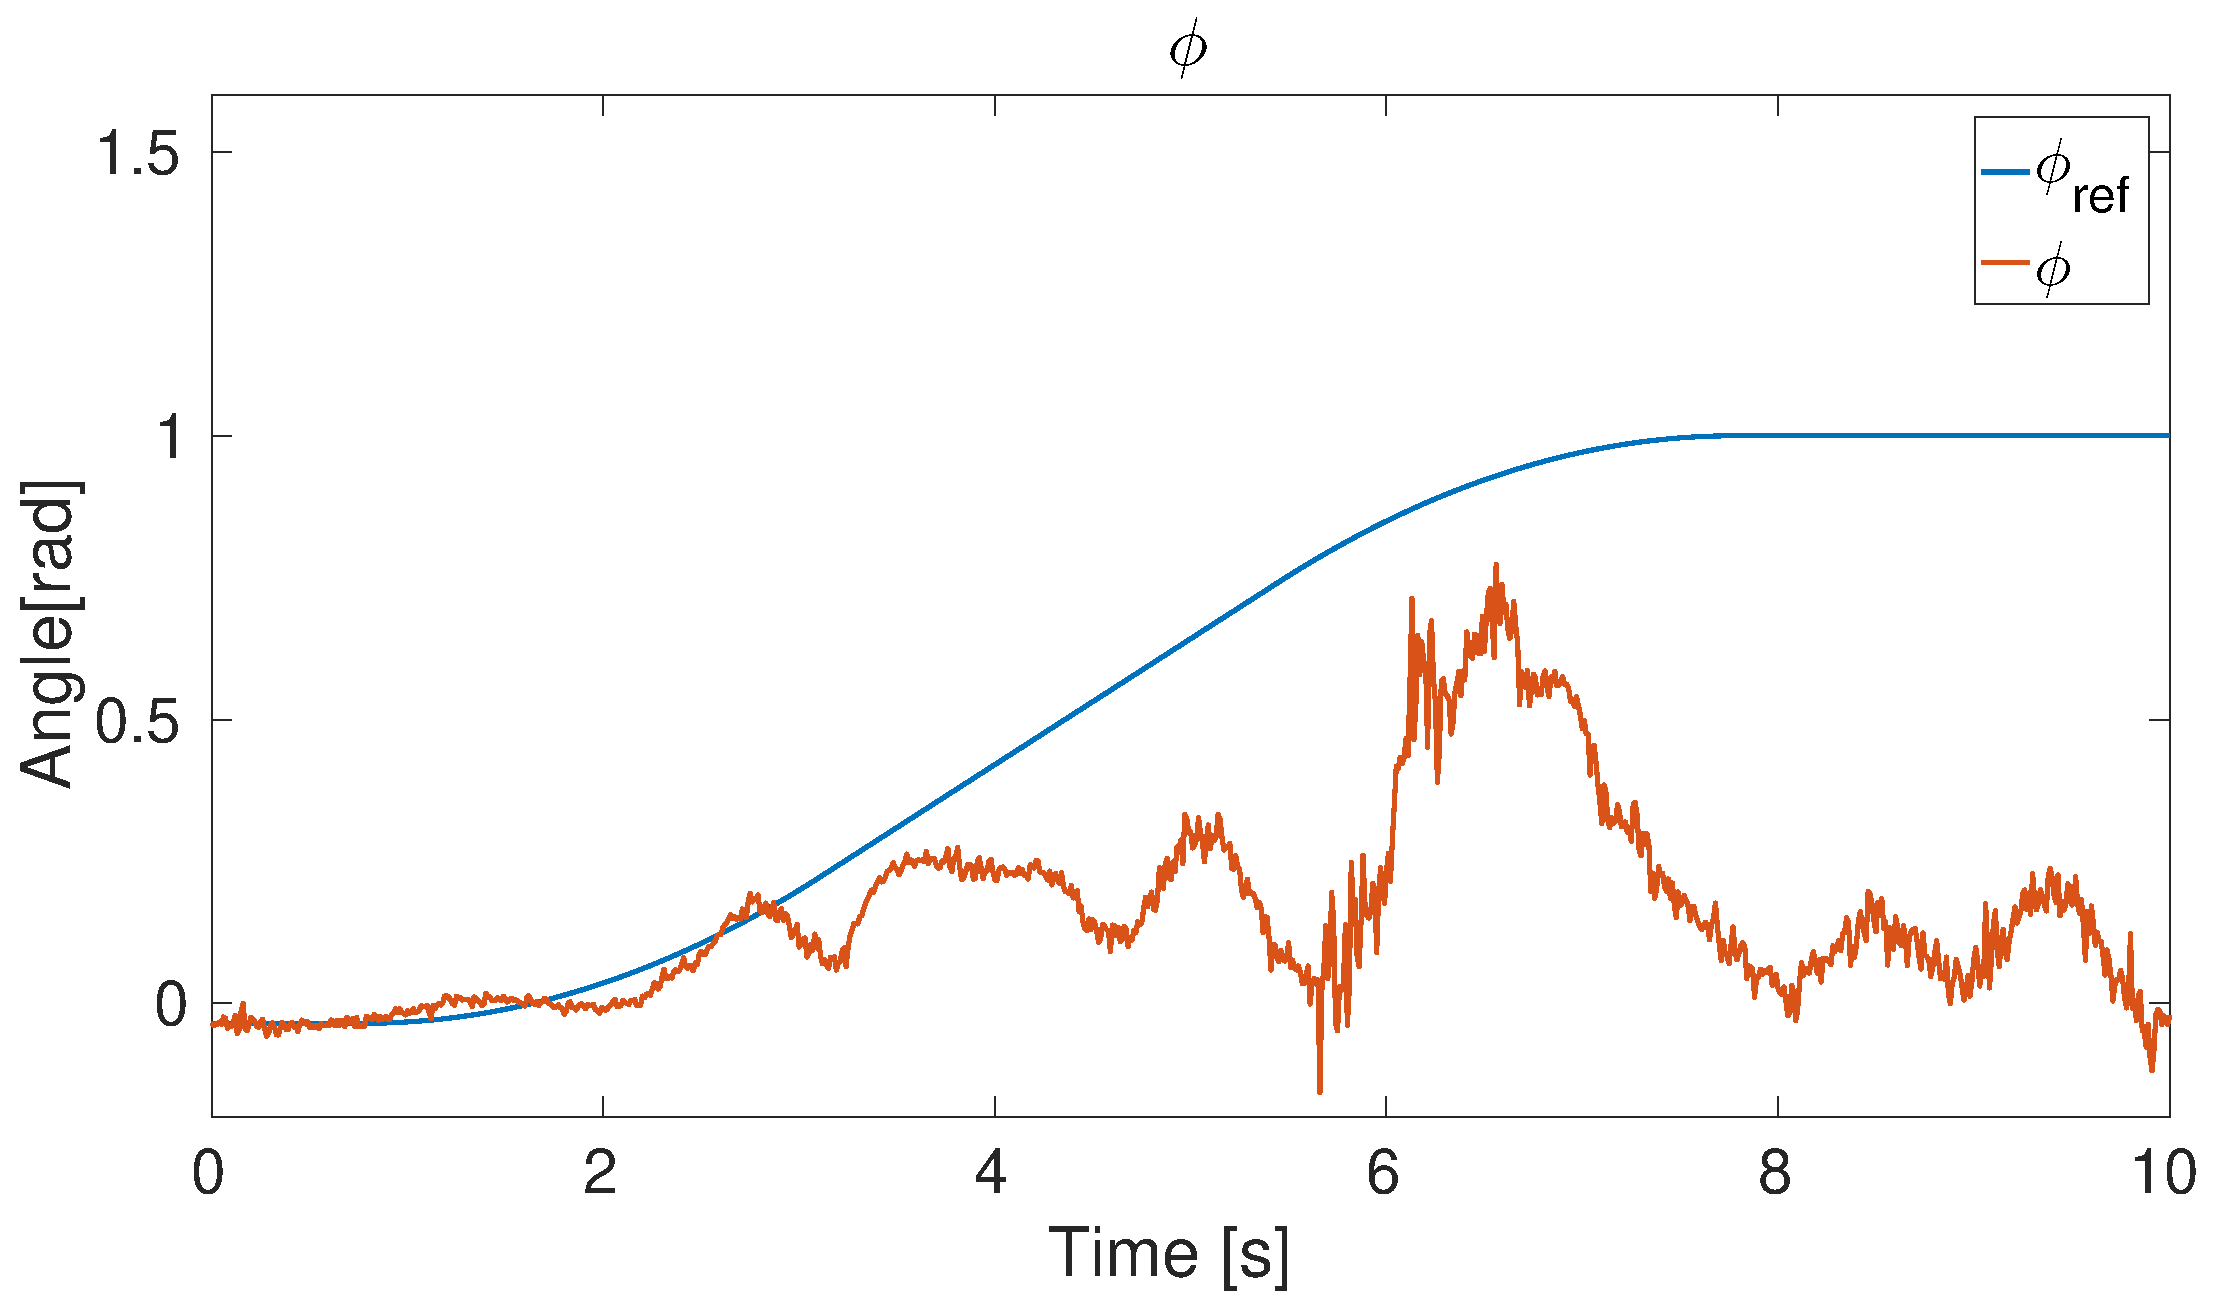
\includegraphics[width=0.4\textwidth]{testStepAllPhis3e10a1}}
  \qquad
  \subfloat[][\label{fig:AppsimStepAllRollAttitude} A smooth step applied to the simulated \abbrROV in $\rollAngle$.]{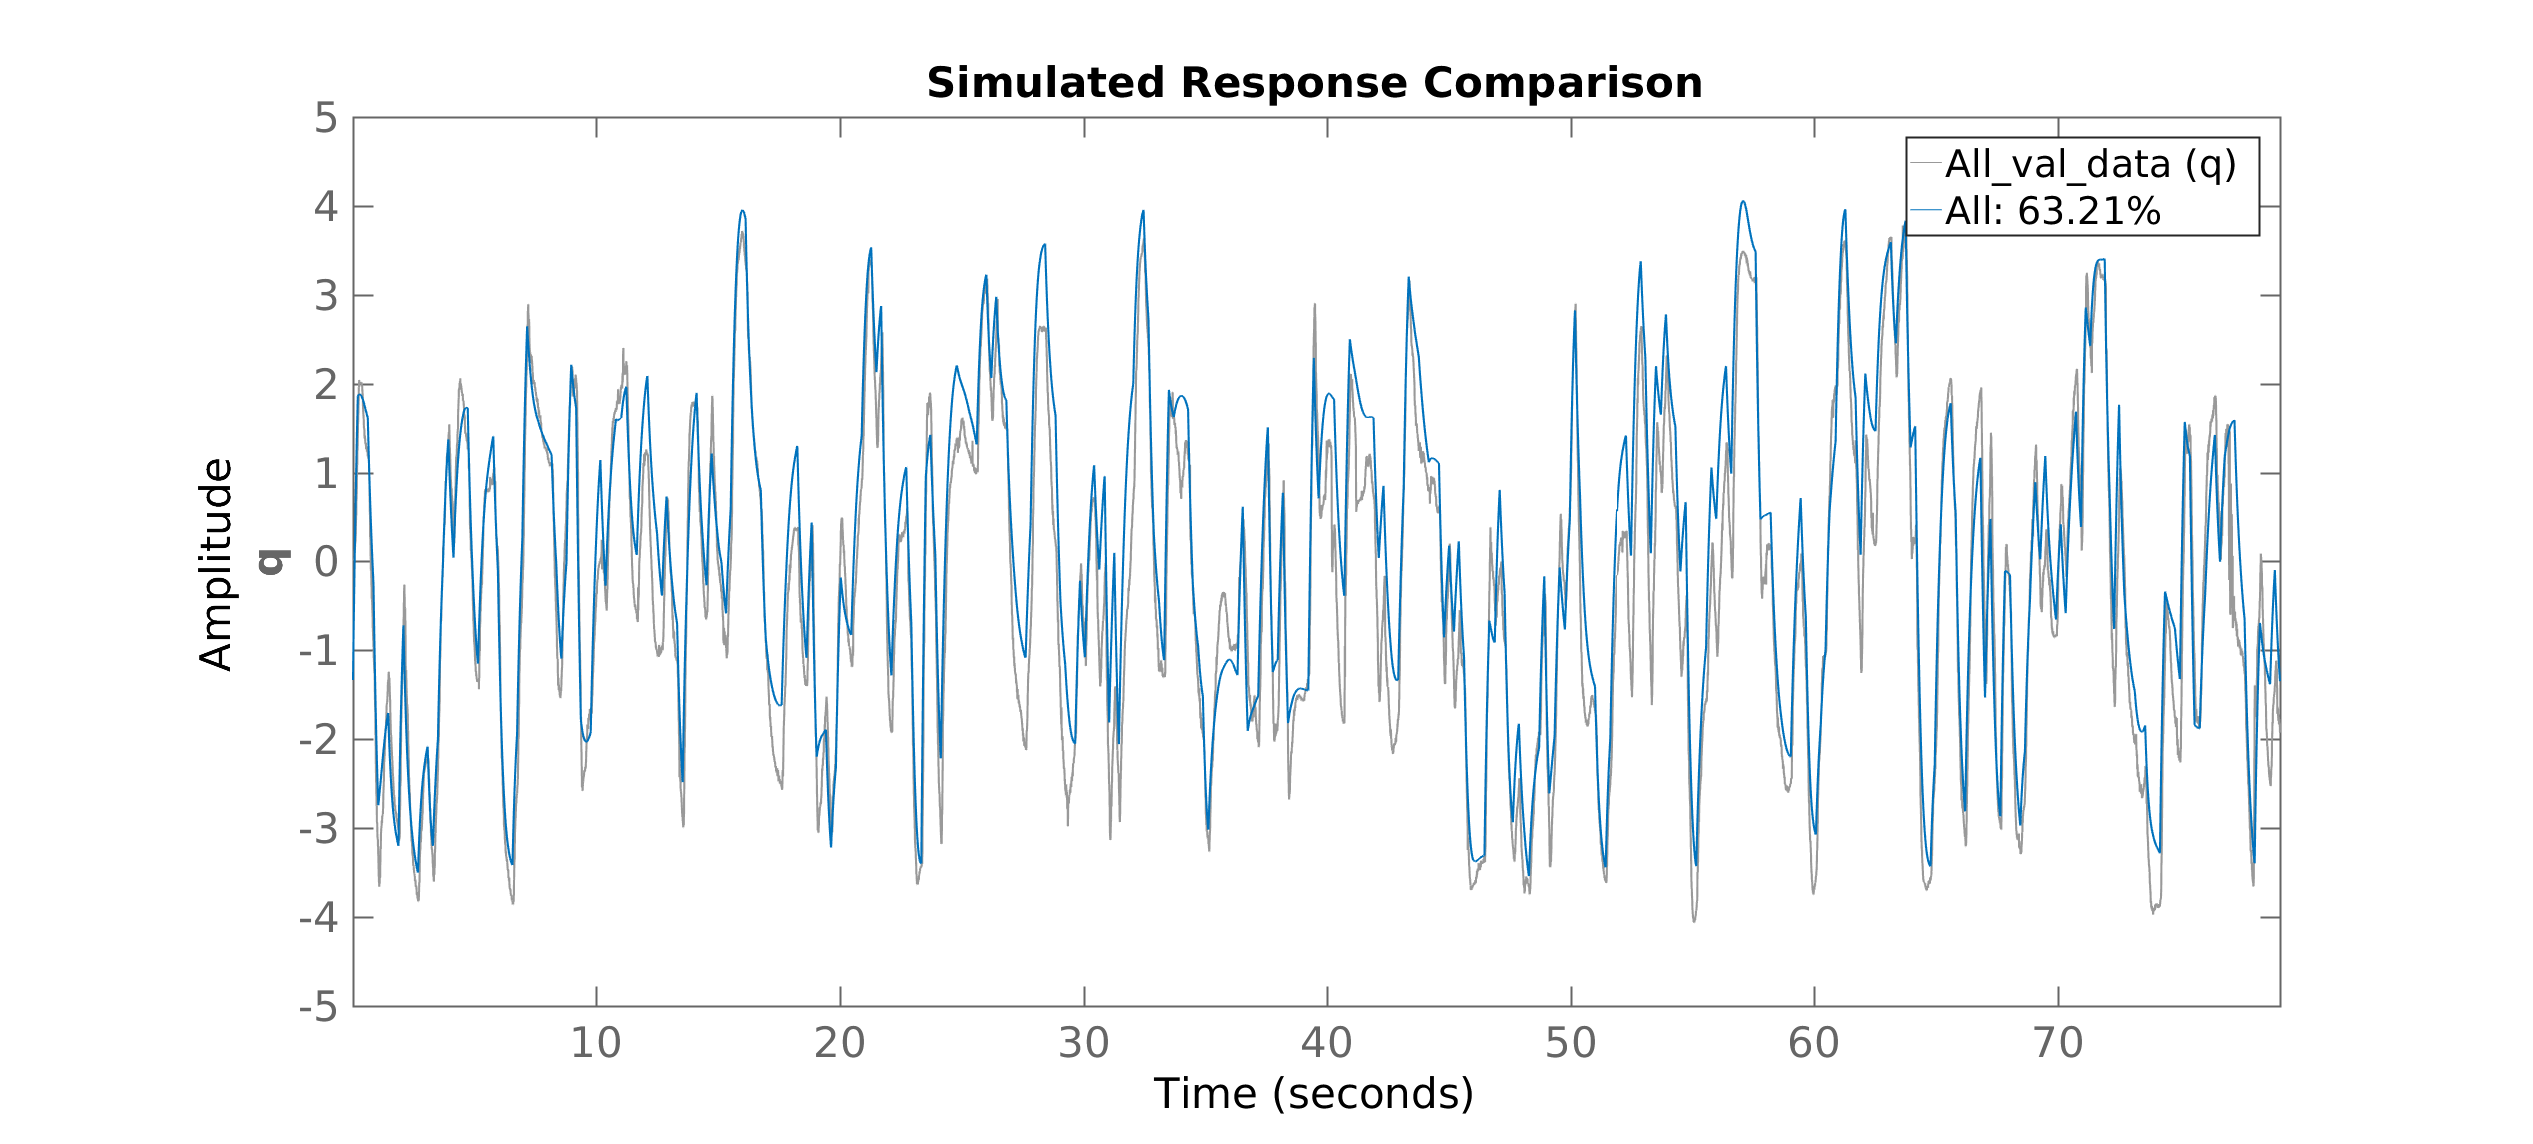
\includegraphics[width=0.4\textwidth]{velocityCompareq}}
  \qquad
  \subfloat[][\label{fig:AppTestStepAllPitchAttitude} A smooth step applied in $\pitchAngle$.]{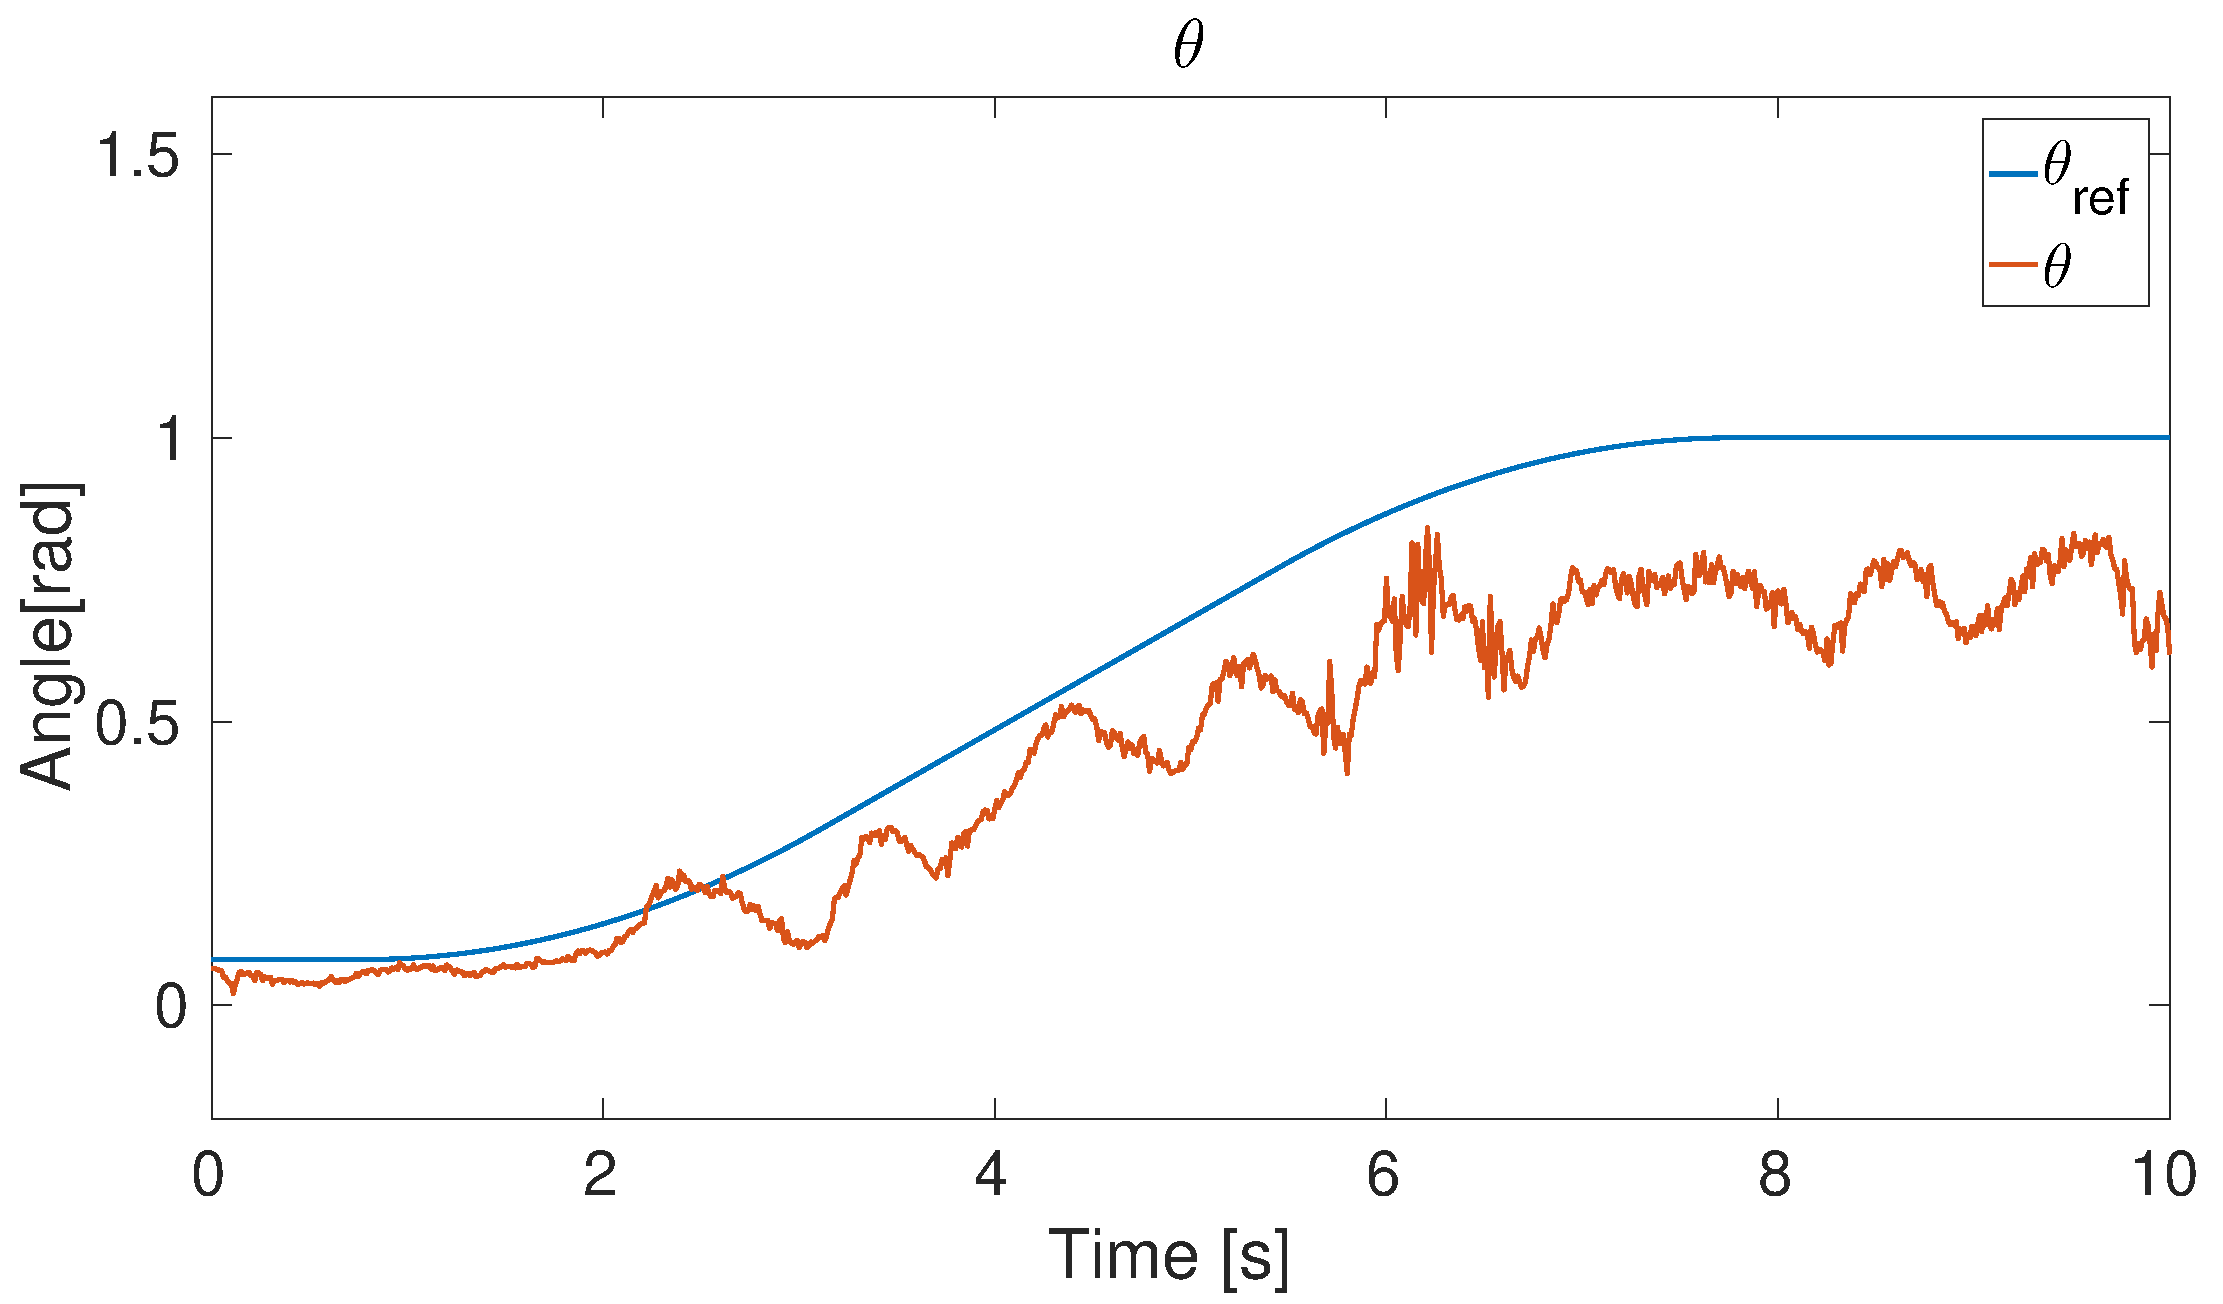
\includegraphics[width=0.4\textwidth]{testStepAllThetas3e10a1}}
  \qquad
  \subfloat[][\label{fig:AppsimStepAllPitchAttitude} A smooth step applied to the simulated \abbrROV in $\pitchAngle$.]{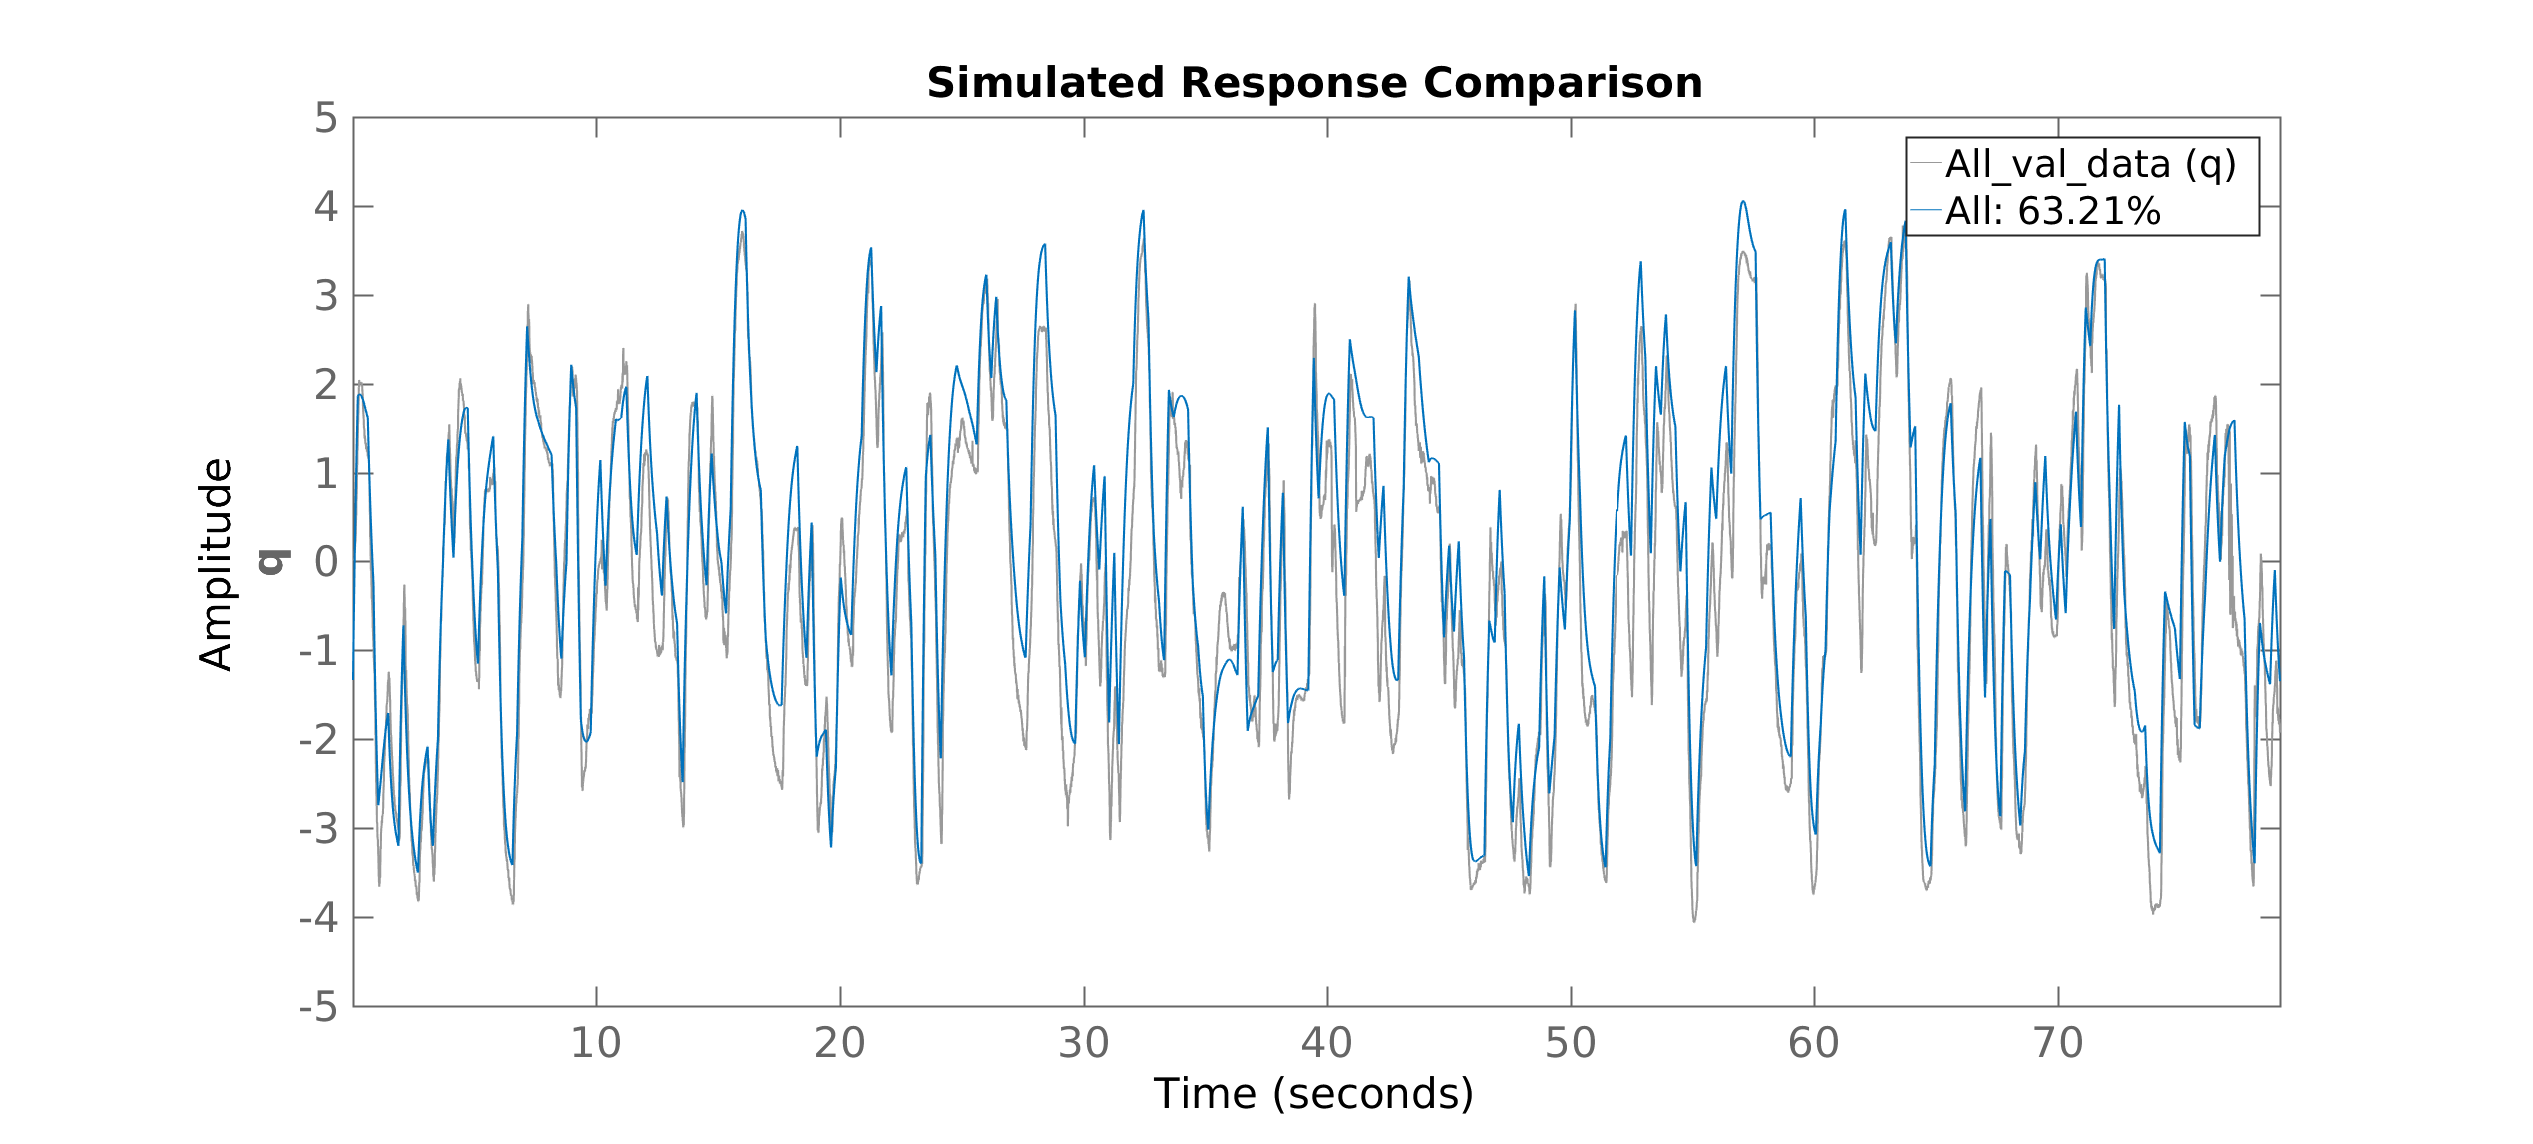
\includegraphics[width=0.4\textwidth]{velocityCompareq}}
  \qquad
  \subfloat[][\label{fig:AppTestStepAllYawAttitude} A smooth step applied in $\yawAngle$.]{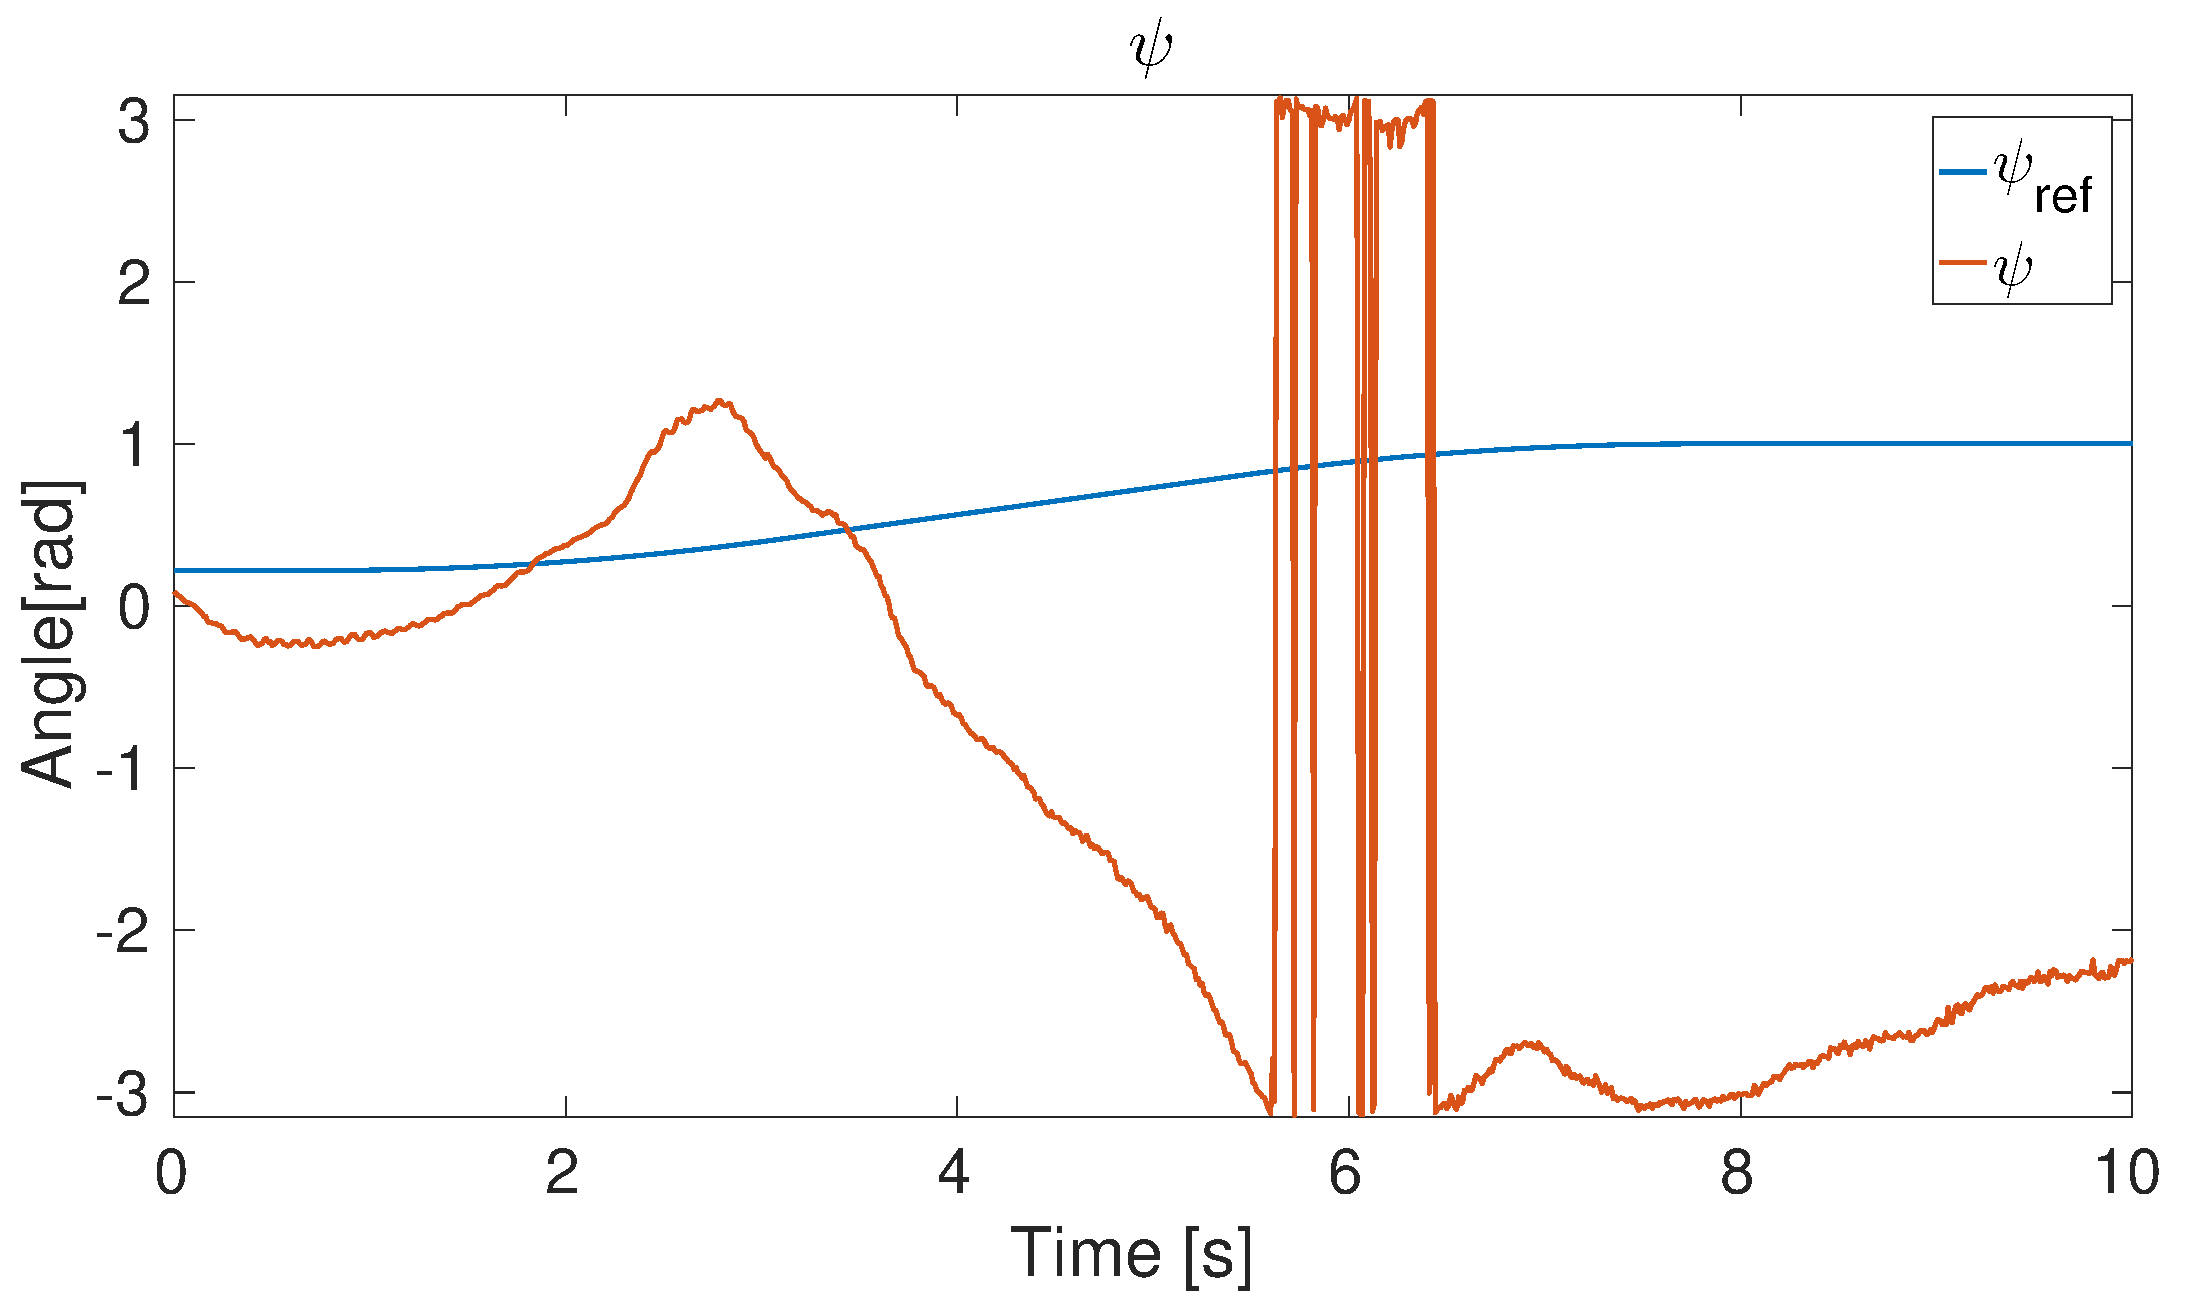
\includegraphics[width=0.4\textwidth]{testStepAllPsis3e10a1}}
  \qquad
  \subfloat[][\label{fig:AppsimStepAllYawAttitude} A smooth step applied to the simulated \abbrROV in $\yawAngle$.]{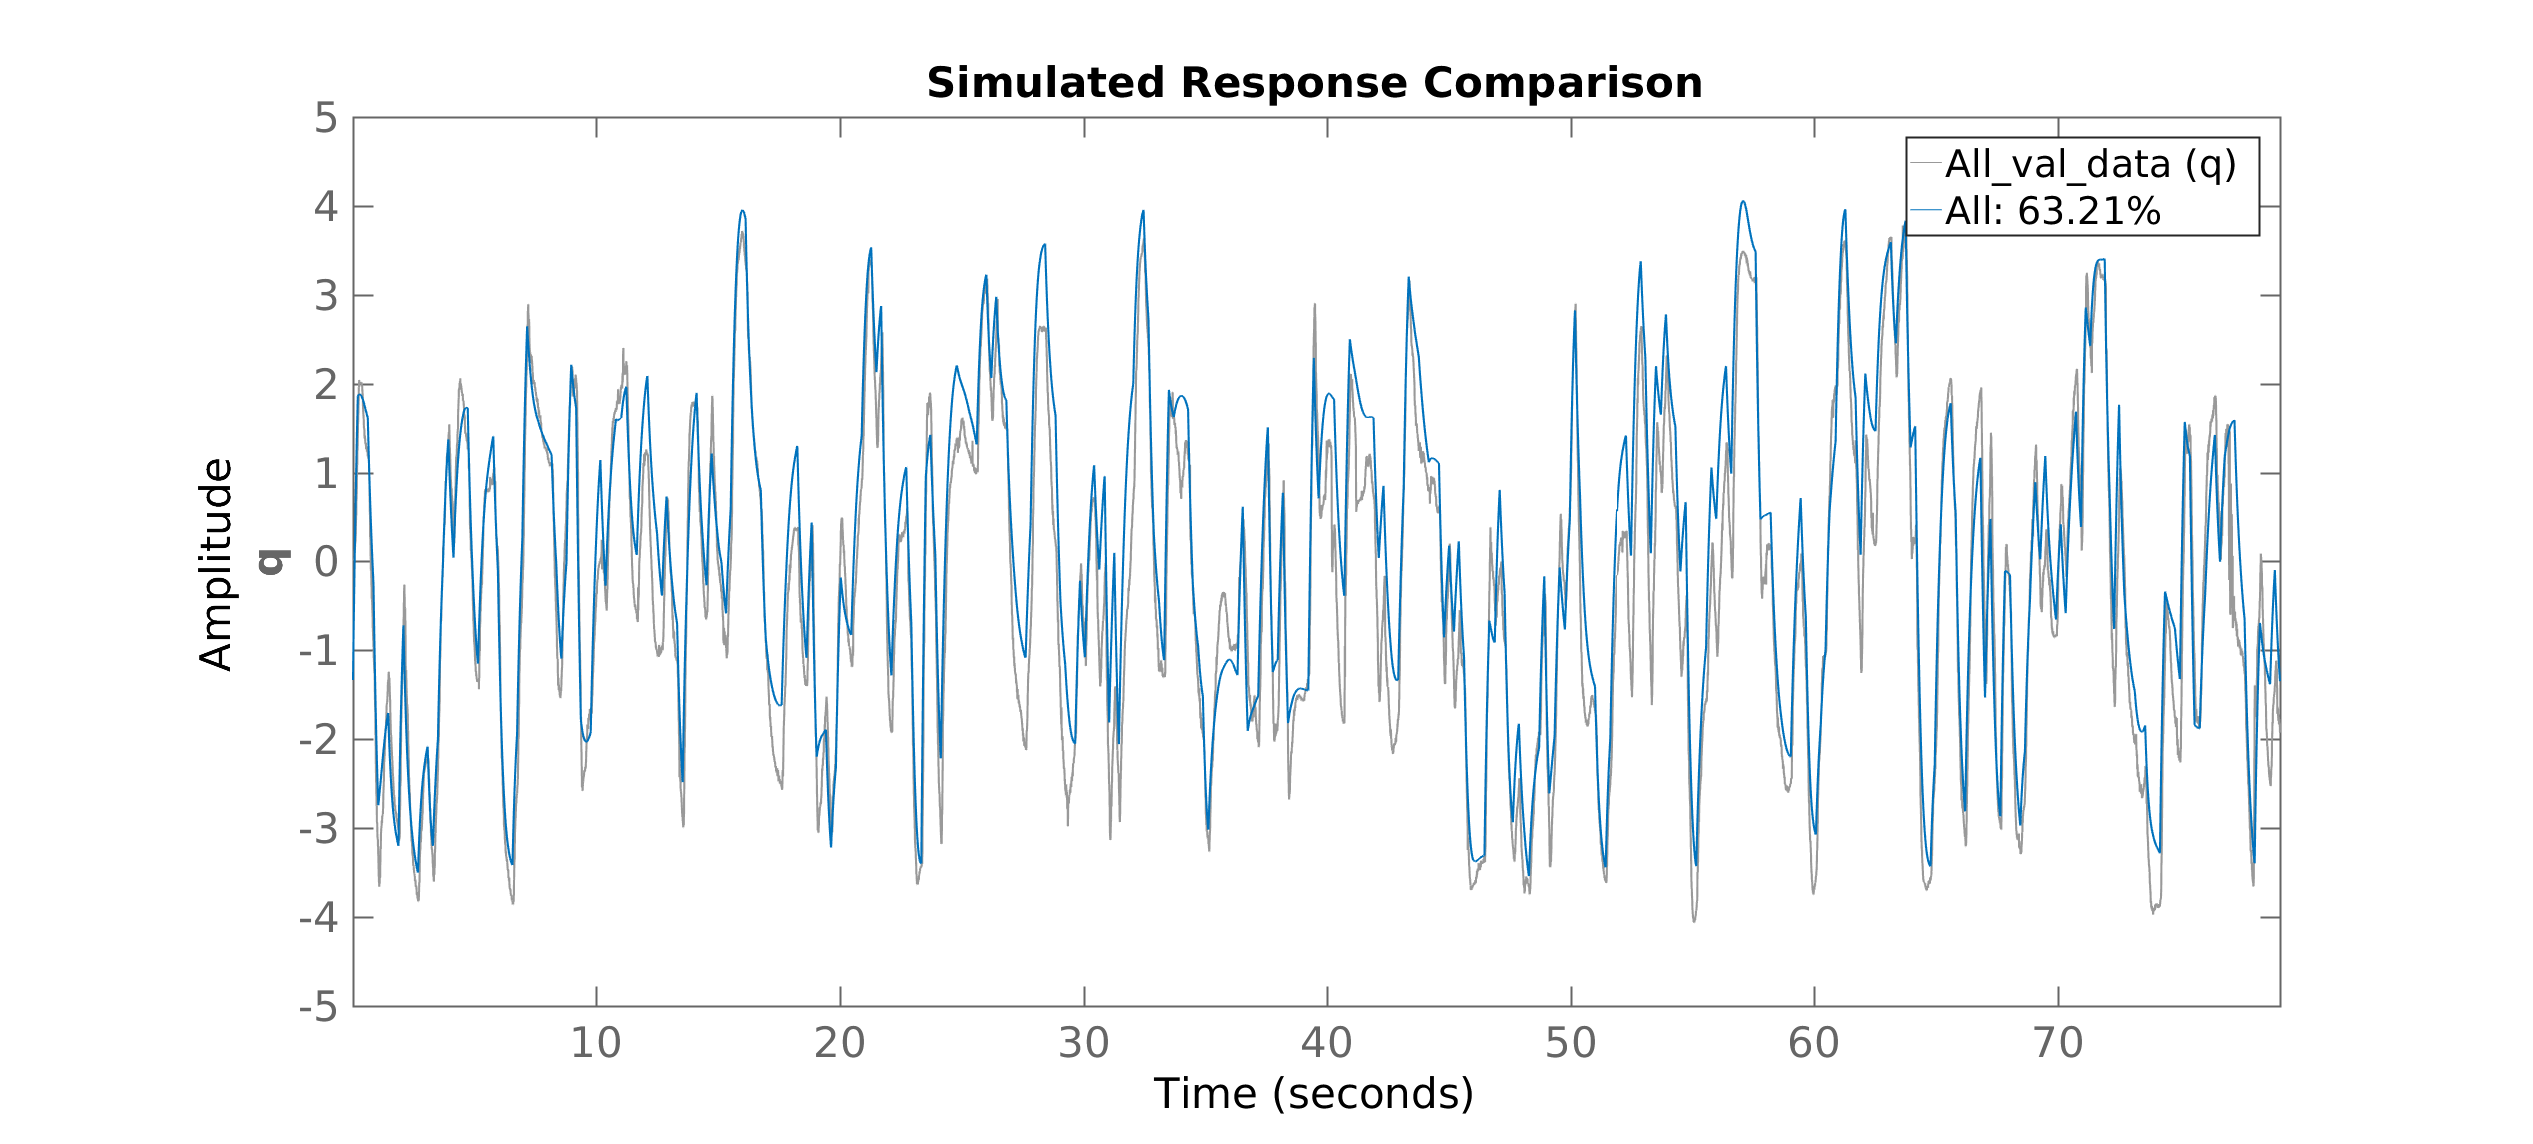
\includegraphics[width=0.4\textwidth]{velocityCompareq}}
  \caption{\label{fig:AppStepAllAttitude}% 
  Smooth steps were applied in all attitude angles at the same time while using the attitude controller.}
\end{figure}

\begin{figure}[tbp]
  \centering
  \subfloat[][\label{fig:ApptestSinRoll} A sine signal with amplitude $1$ and frequency $0.5\hertz$ applied in $\rollAngle$.]{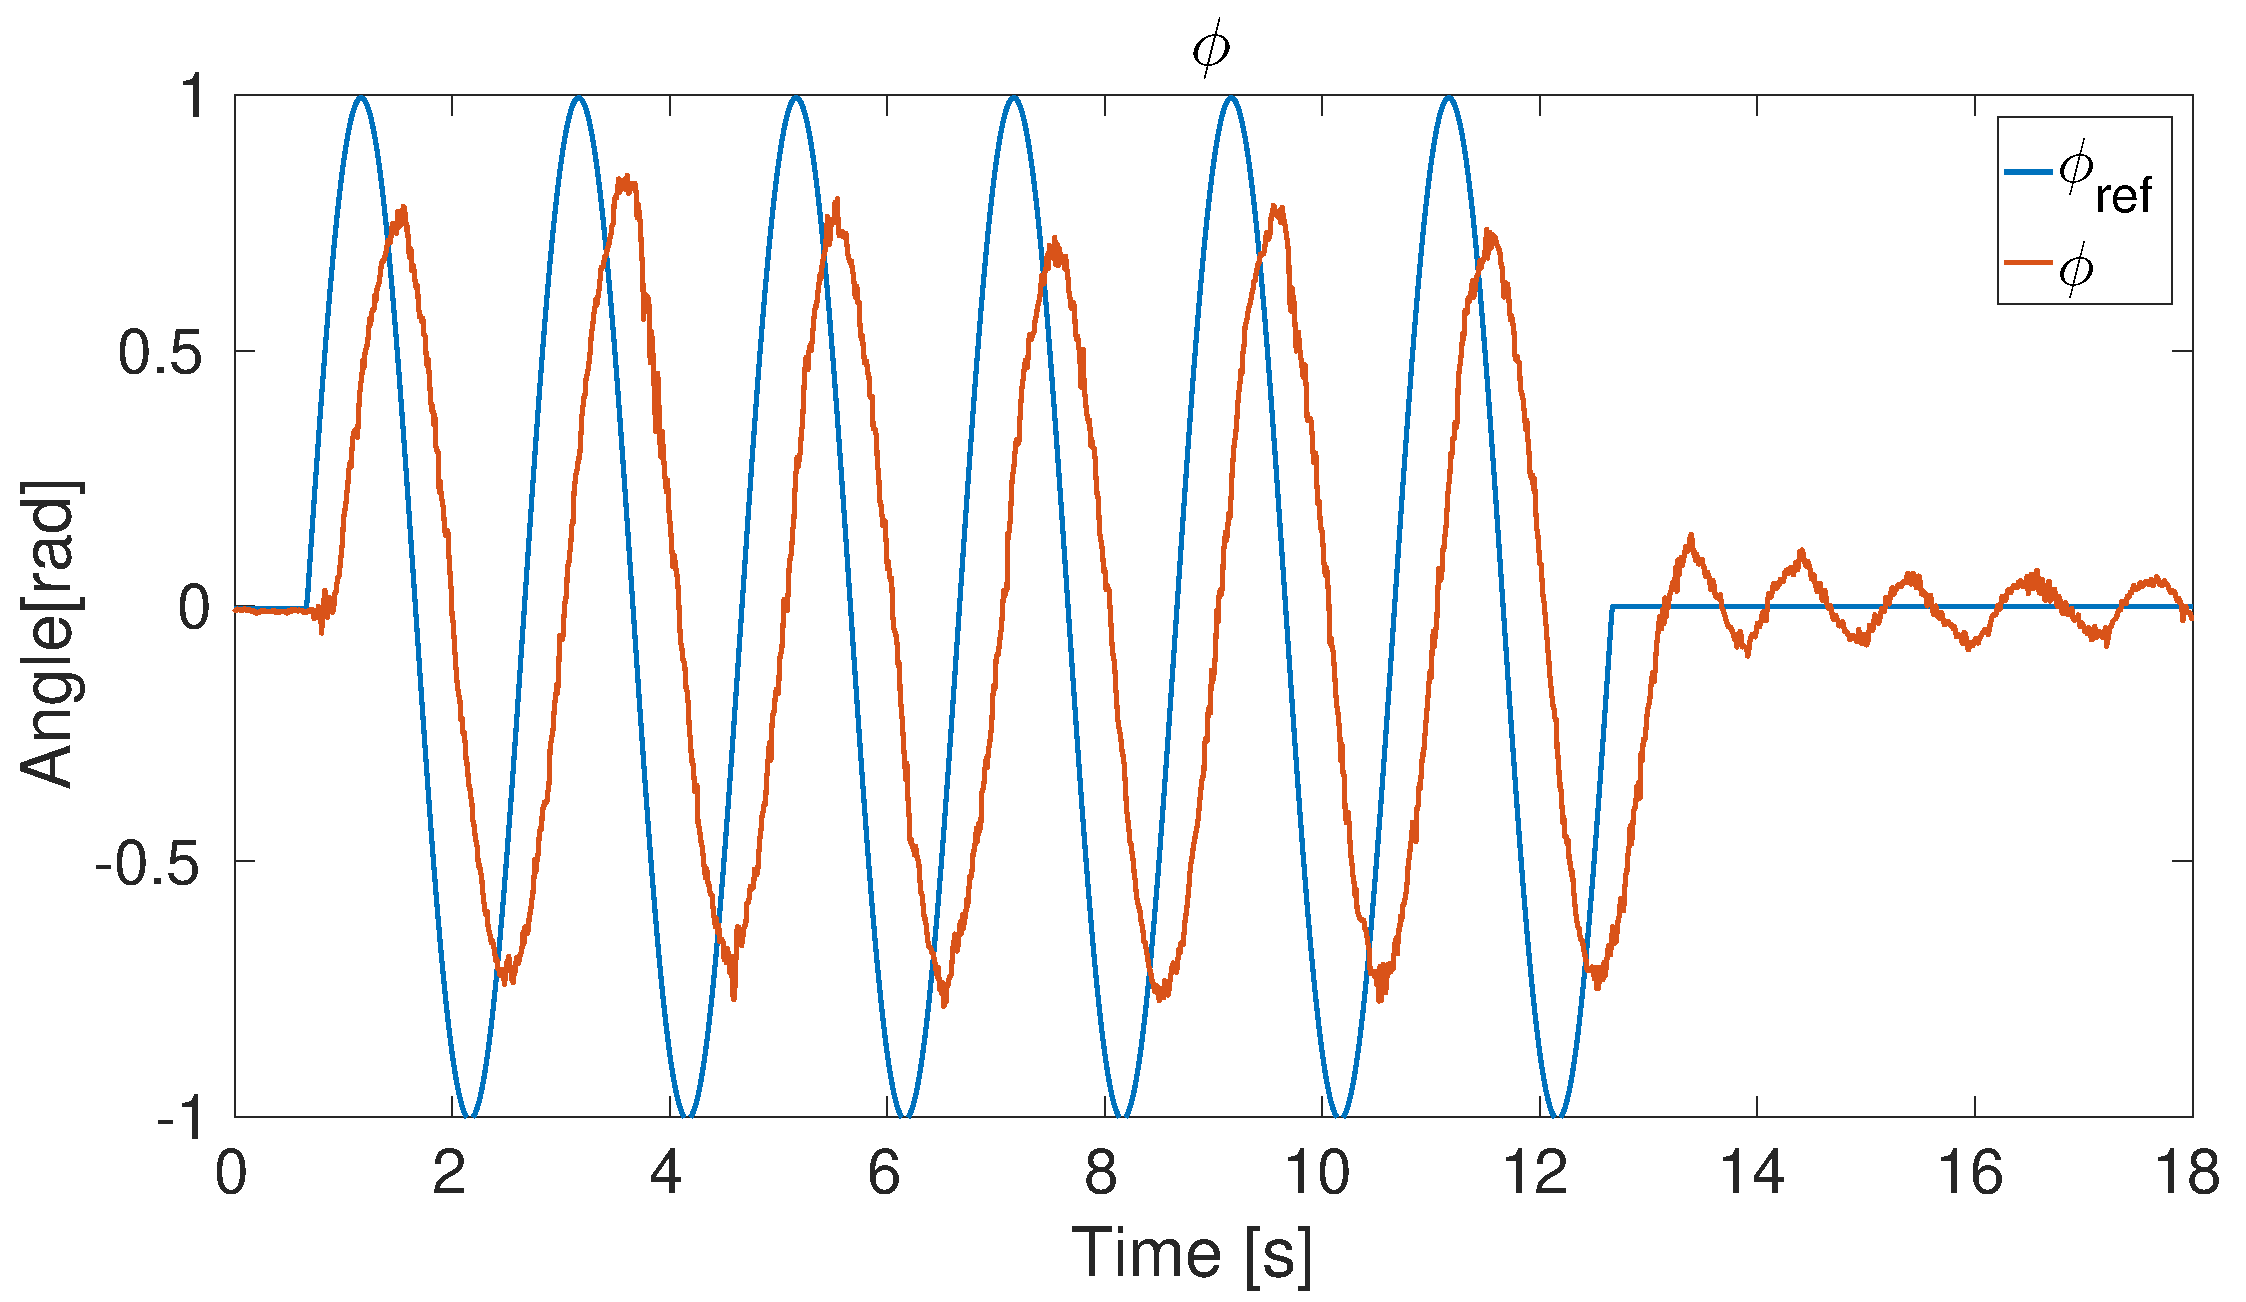
\includegraphics[width=0.4\textwidth]{testSinPhiA1}}
  \qquad
  \subfloat[][\label{fig:AppsimSinRoll} A sine signal with amplitude $1$ and frequency $0.5\hertz$ applied to the simulated \abbrROV in $\rollAngle$.]{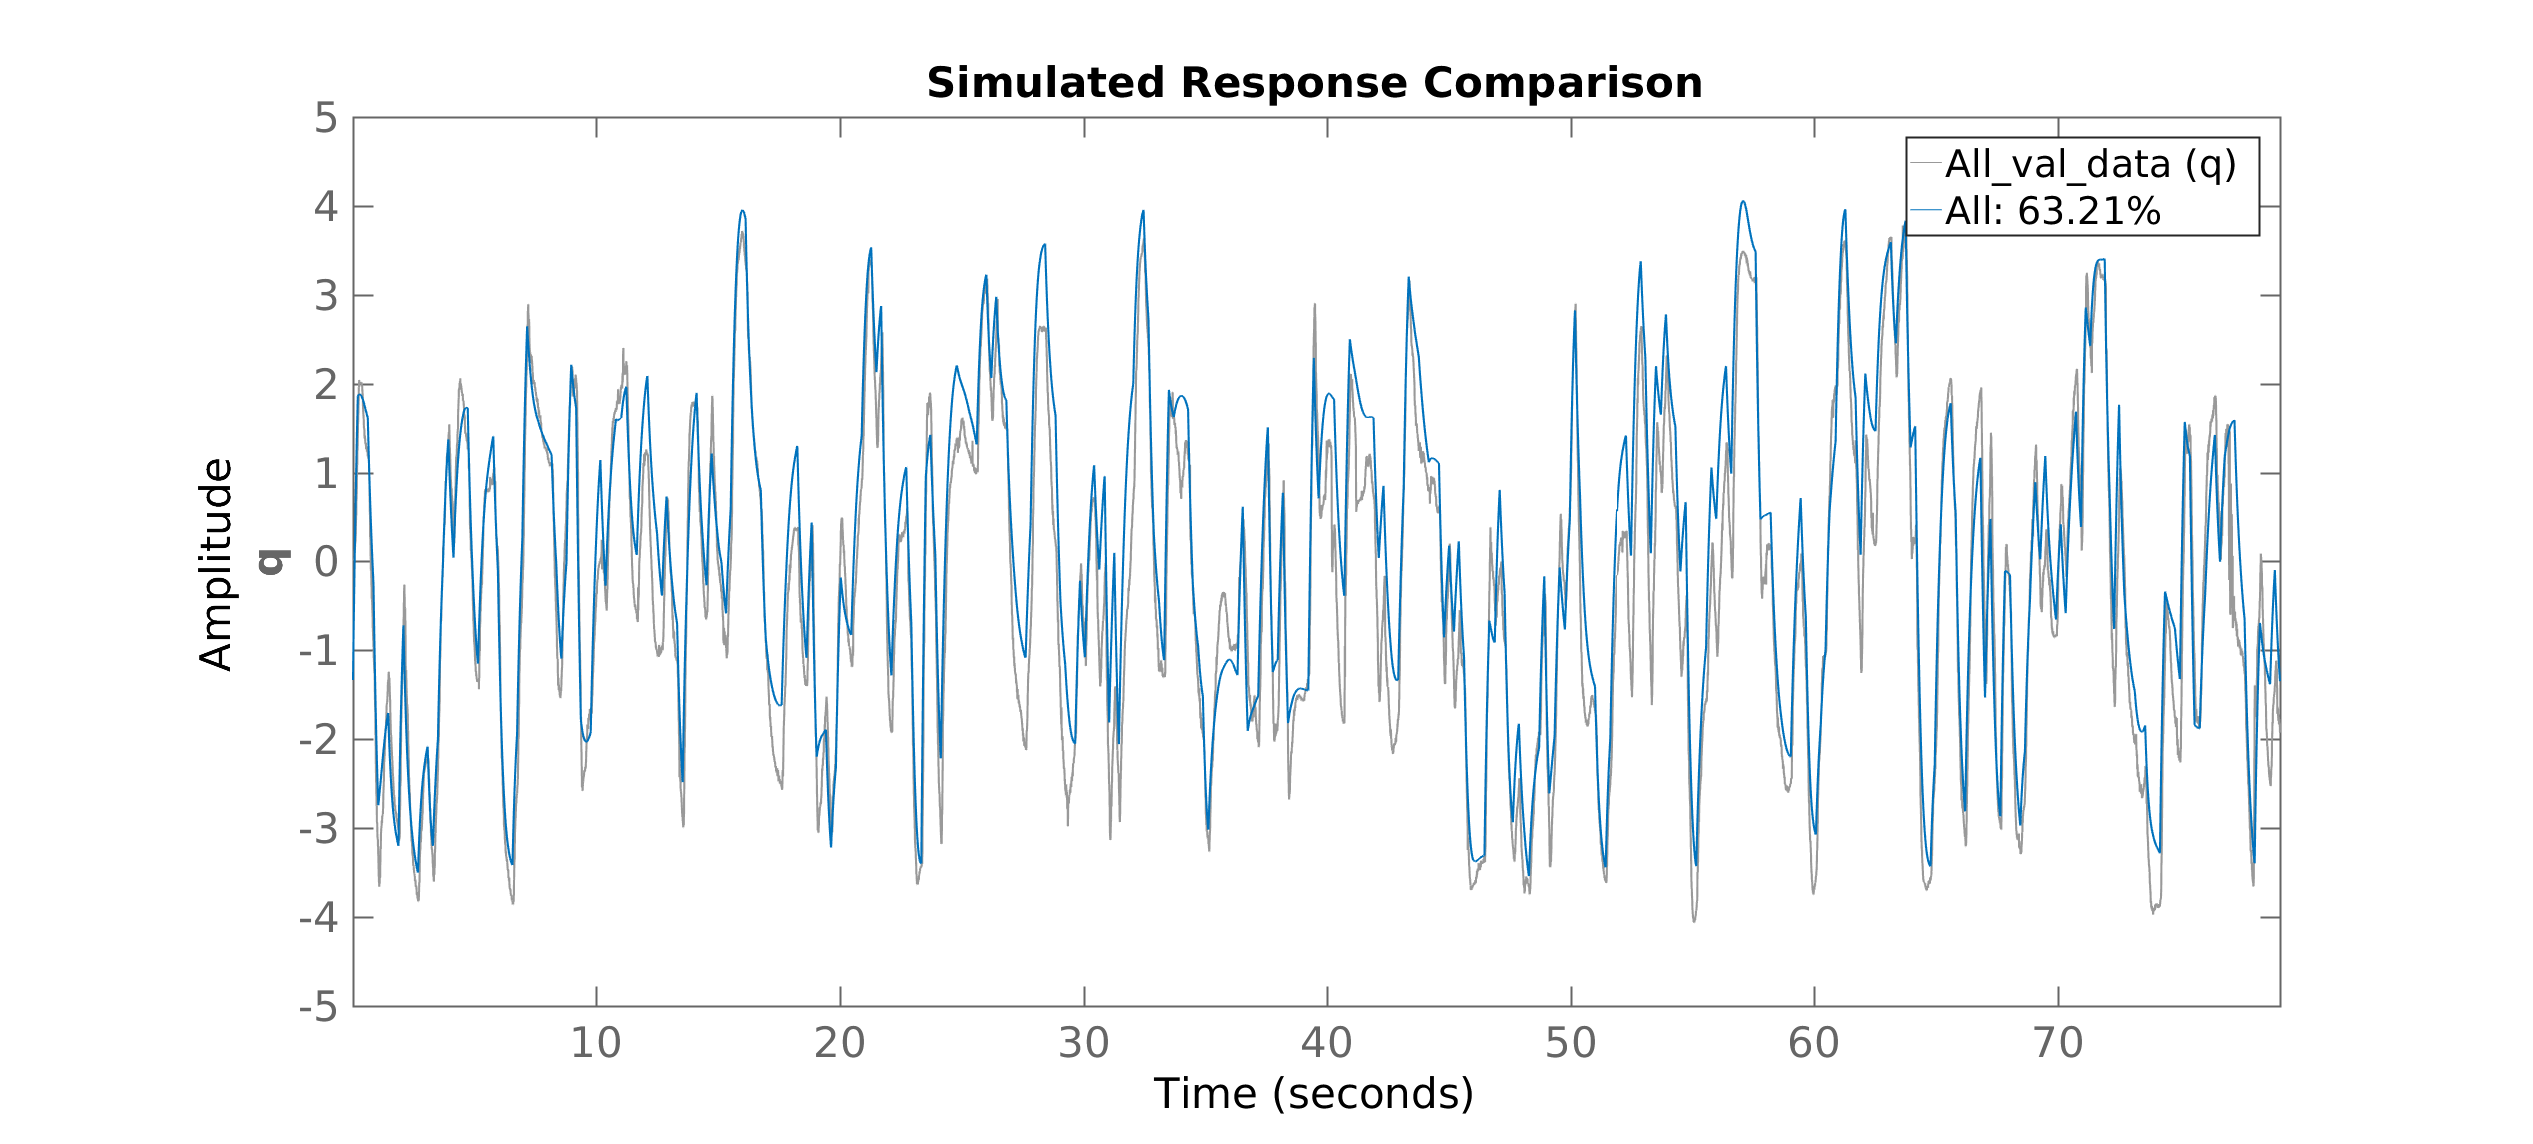
\includegraphics[width=0.4\textwidth]{velocityCompareq}}
  \qquad
  \subfloat[][\label{fig:ApptestSinPitch} A sine signal with amplitude $1$ and frequency $0.5\hertz$ applied in $\pitchAngle$.]{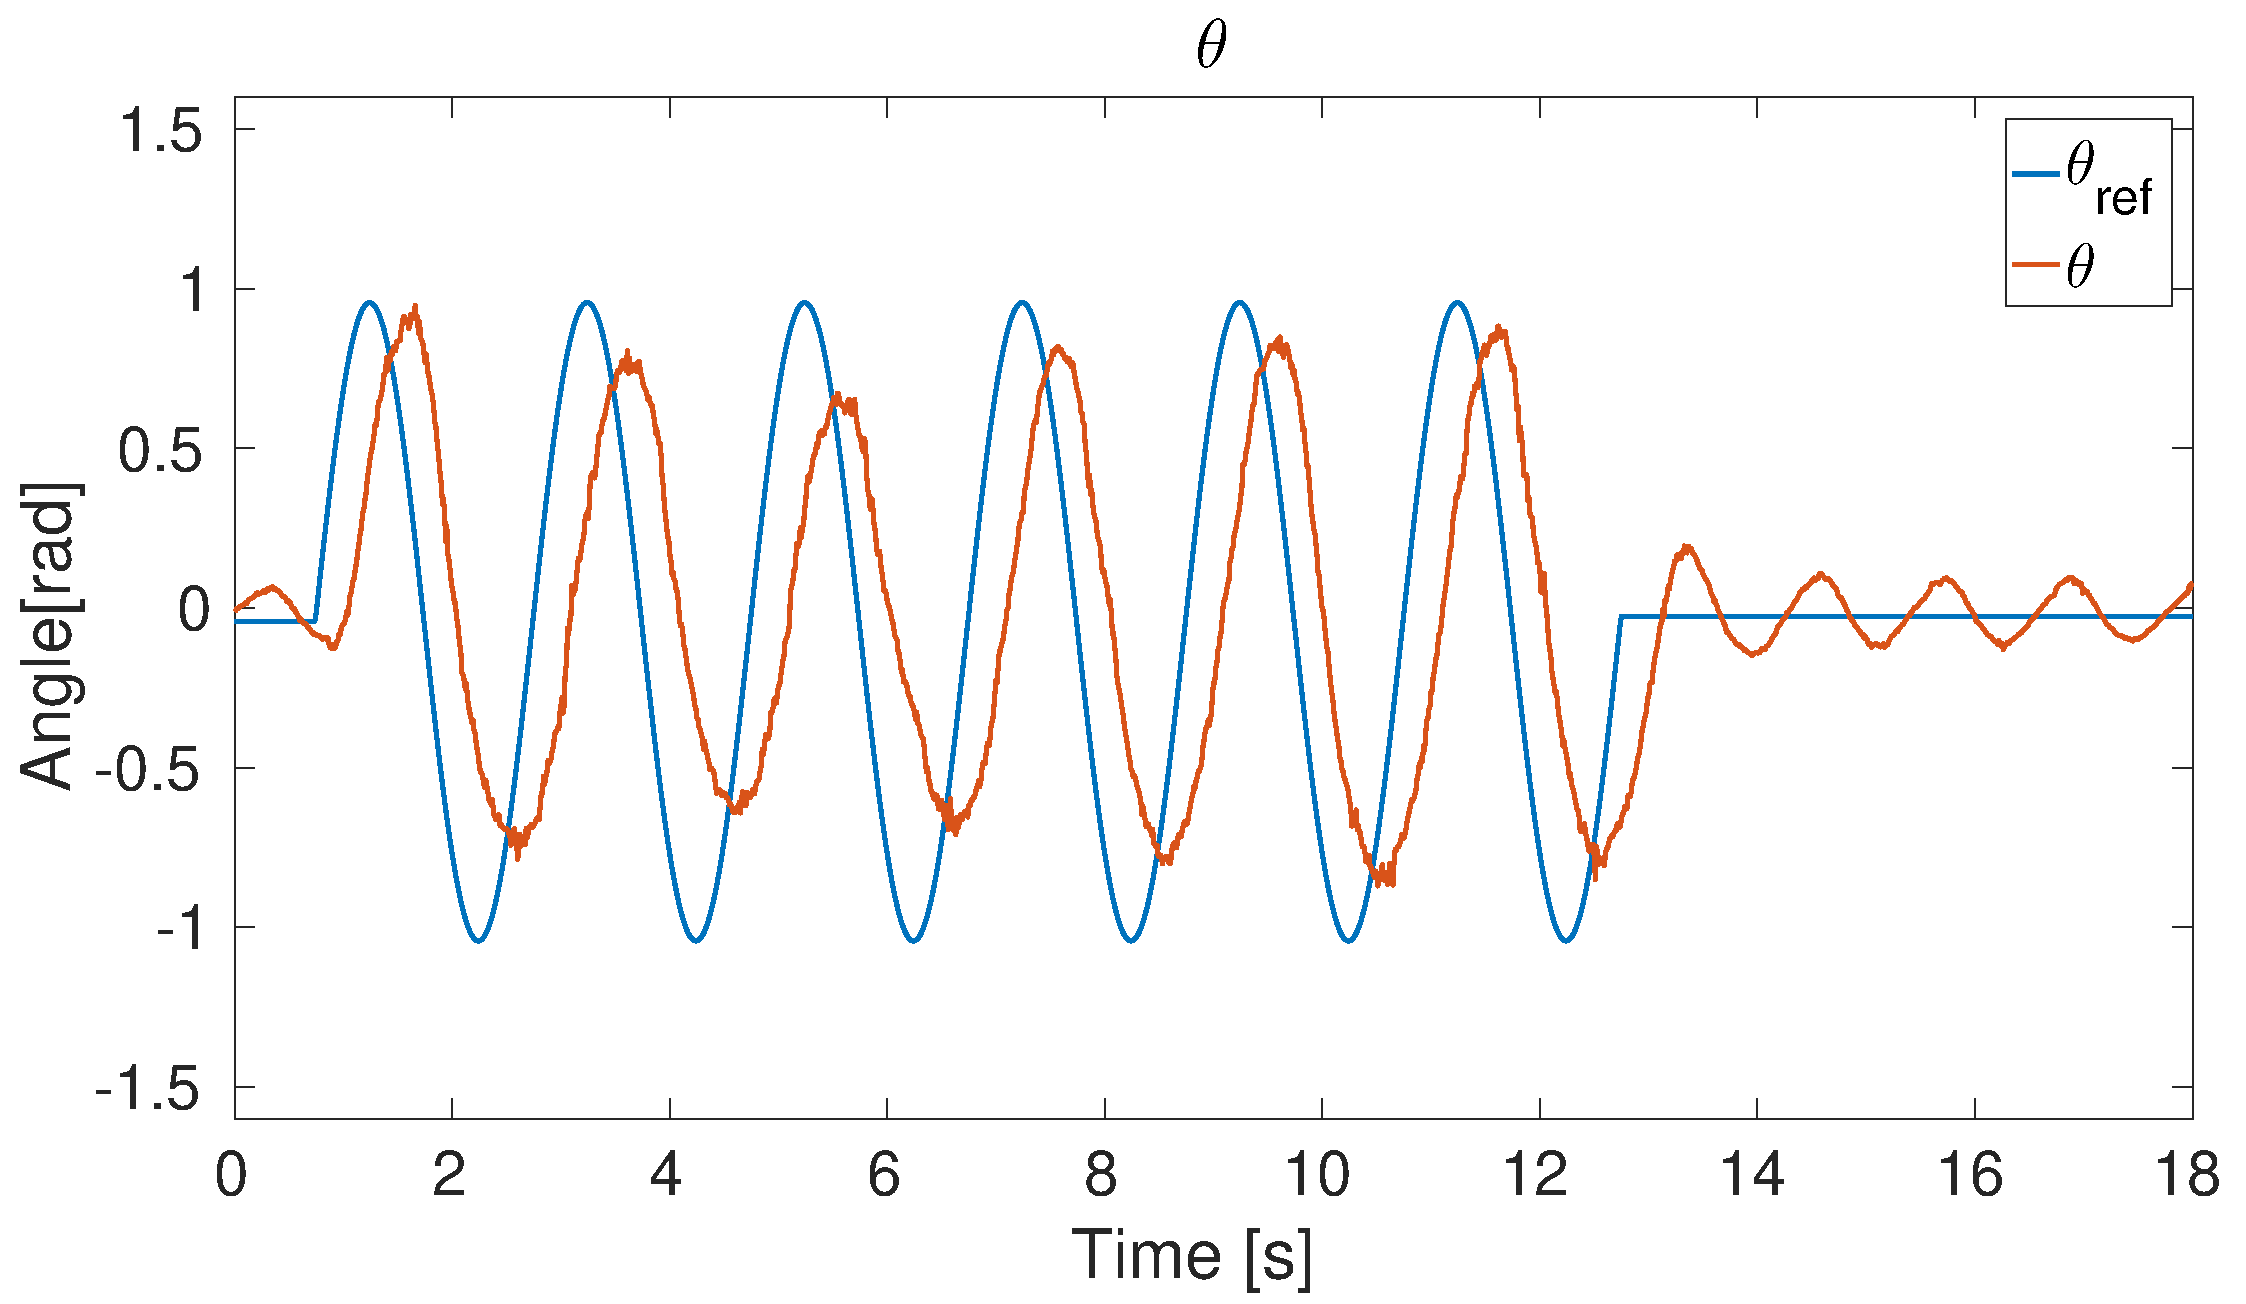
\includegraphics[width=0.4\textwidth]{testSinThetaA1}}
  \qquad
  \subfloat[][\label{fig:AppsimSinPitch} A sine signal with amplitude $1$ and frequency $0.5\hertz$ applied to the simulated \abbrROV in $\pitchAngle$.]{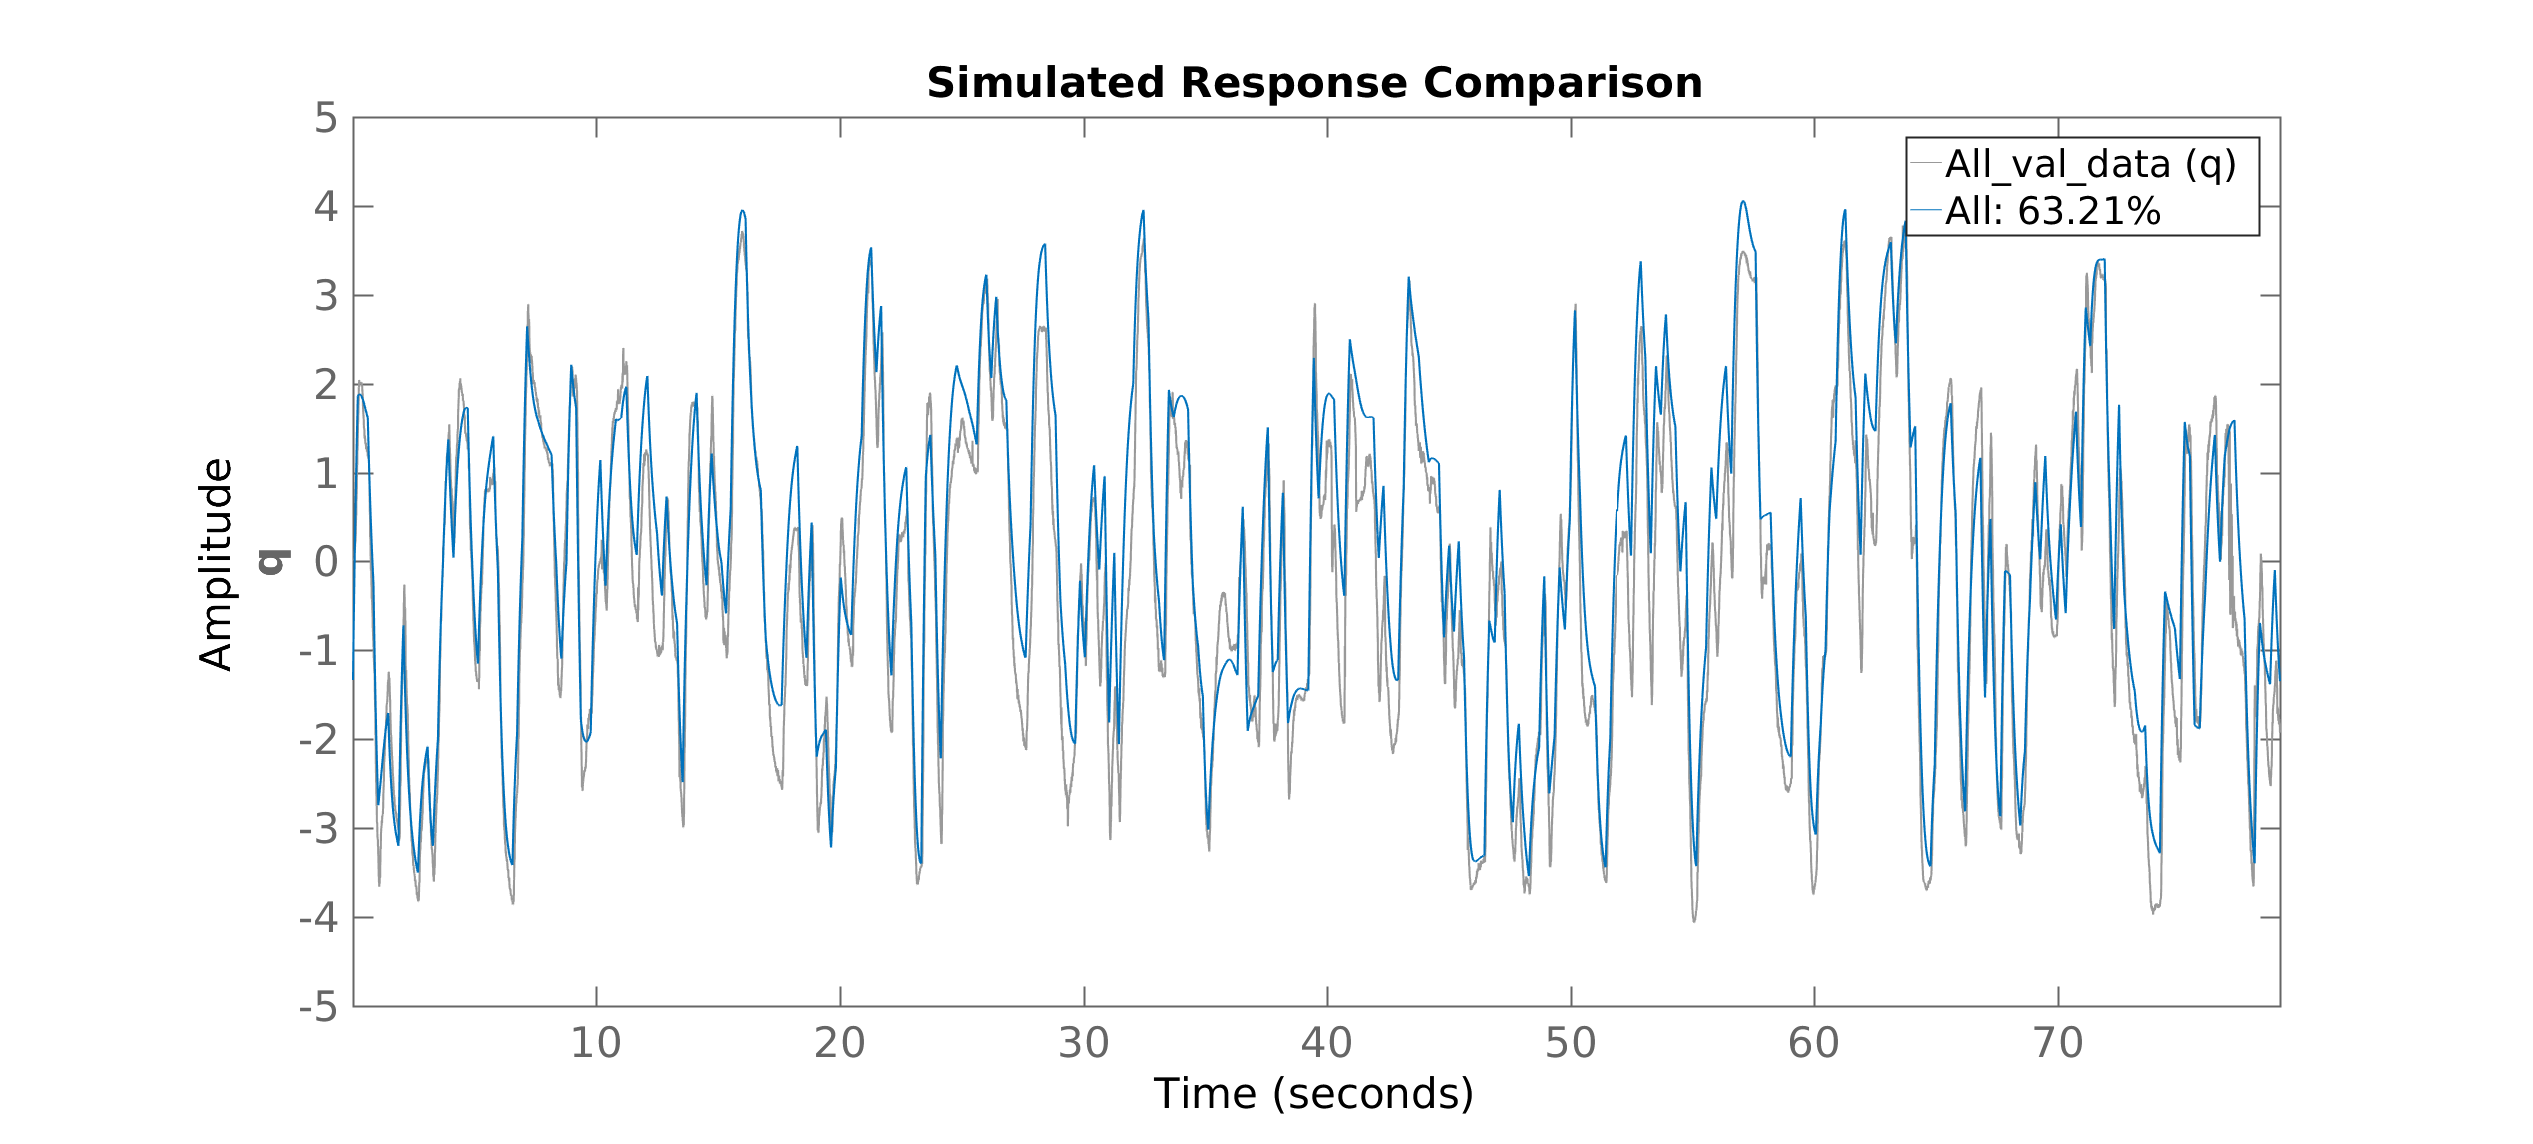
\includegraphics[width=0.4\textwidth]{velocityCompareq}}
  \qquad
  \subfloat[][\label{fig:ApptestSinYaw} A sine signal with amplitude $1$ and frequency $0.5\hertz$ applied in $\yawAngle$.]{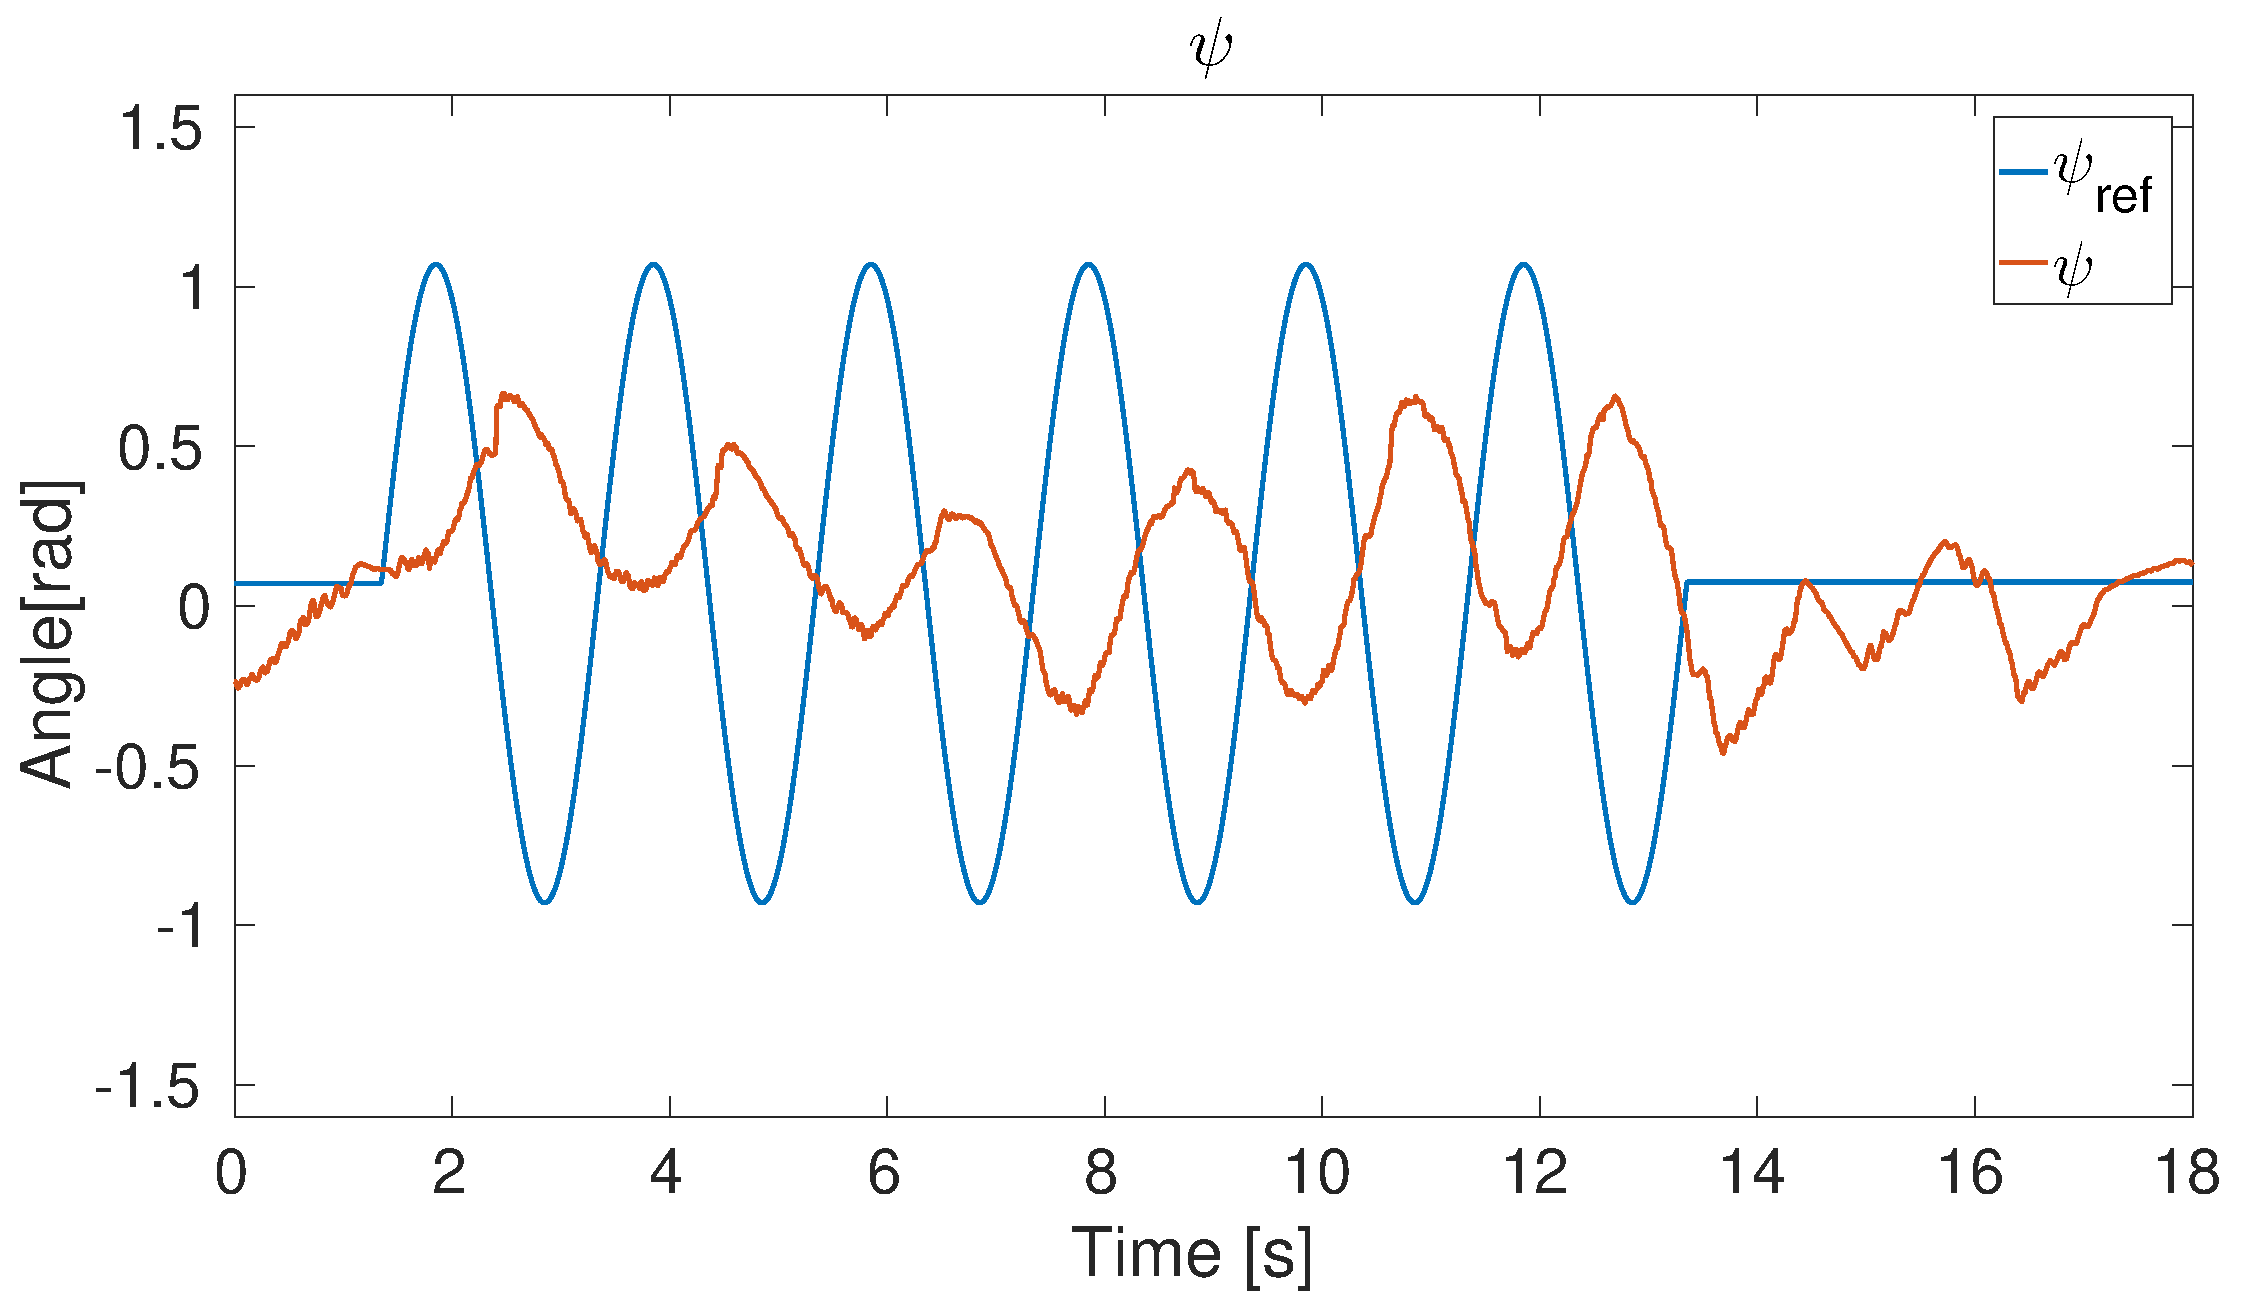
\includegraphics[width=0.4\textwidth]{testSinPsiA1}}
  \qquad
  \subfloat[][\label{fig:AppsimSinYaw} A sine signal with amplitude $1$ and frequency $0.5\hertz$ applied to the simulated \abbrROV in $\yawAngle$.]{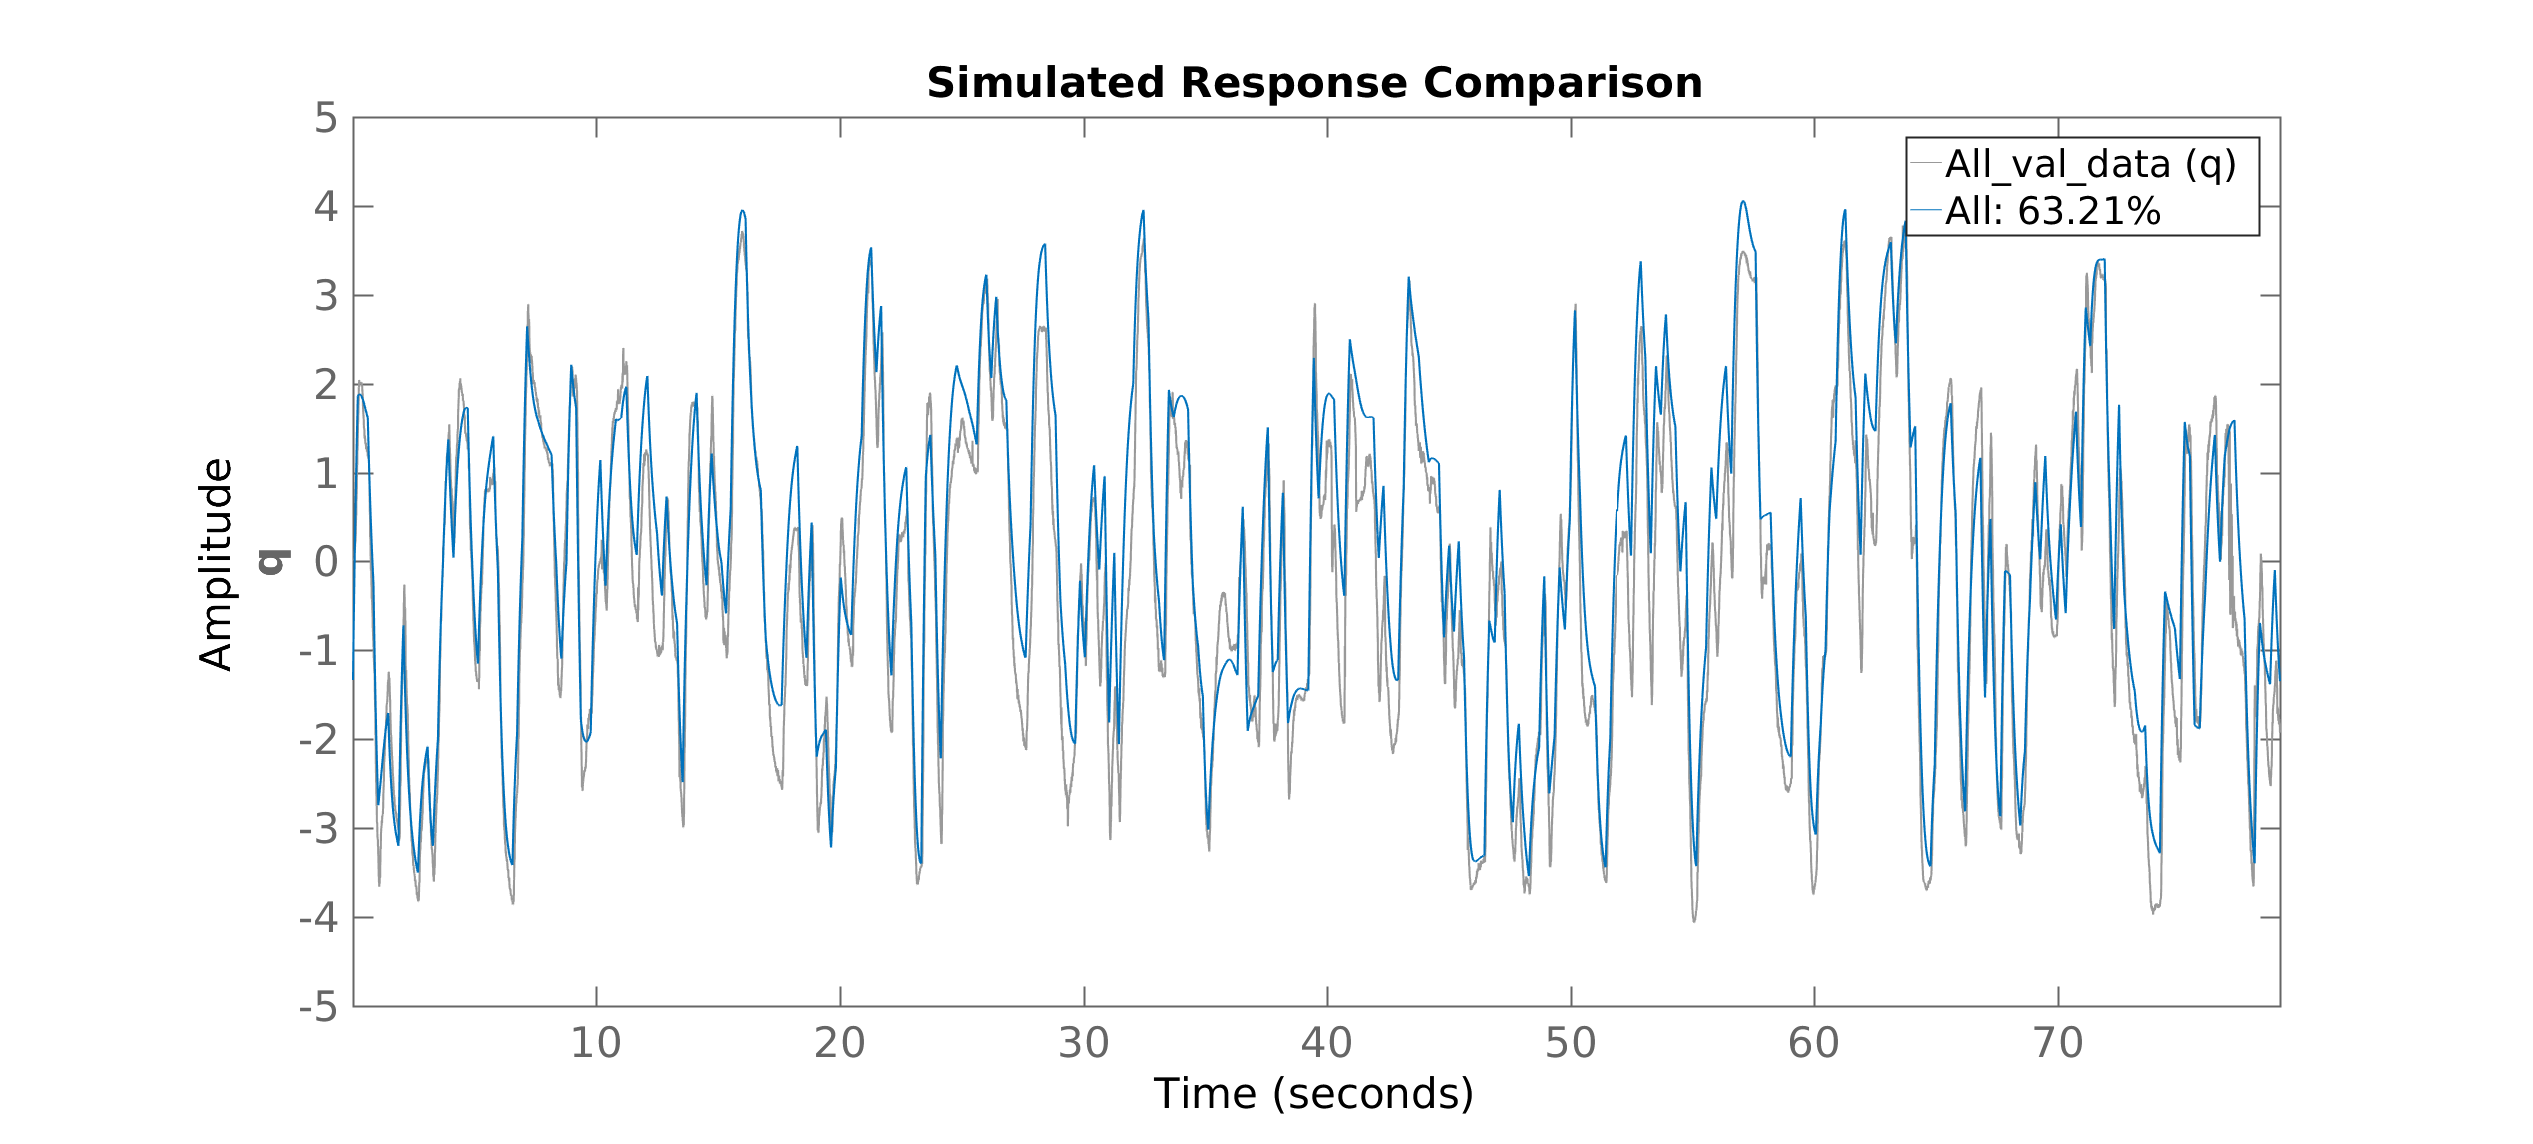
\includegraphics[width=0.4\textwidth]{velocityCompareq}}
    \caption{\label{fig:AppSin1Attitude}% 
   A sine signal was applied in one attitude angle at a time while using the attitude controller. While a sine signal was applied in one attitude angle the other attitude angles were not controlled.}
\end{figure}

\begin{figure}
\centering
  \subfloat[][\label{fig:ApptestSinAllRollAttitude} A sine signal with amplitude $1$ and frequency $0.5\hertz$ applied in $\rollAngle$.]{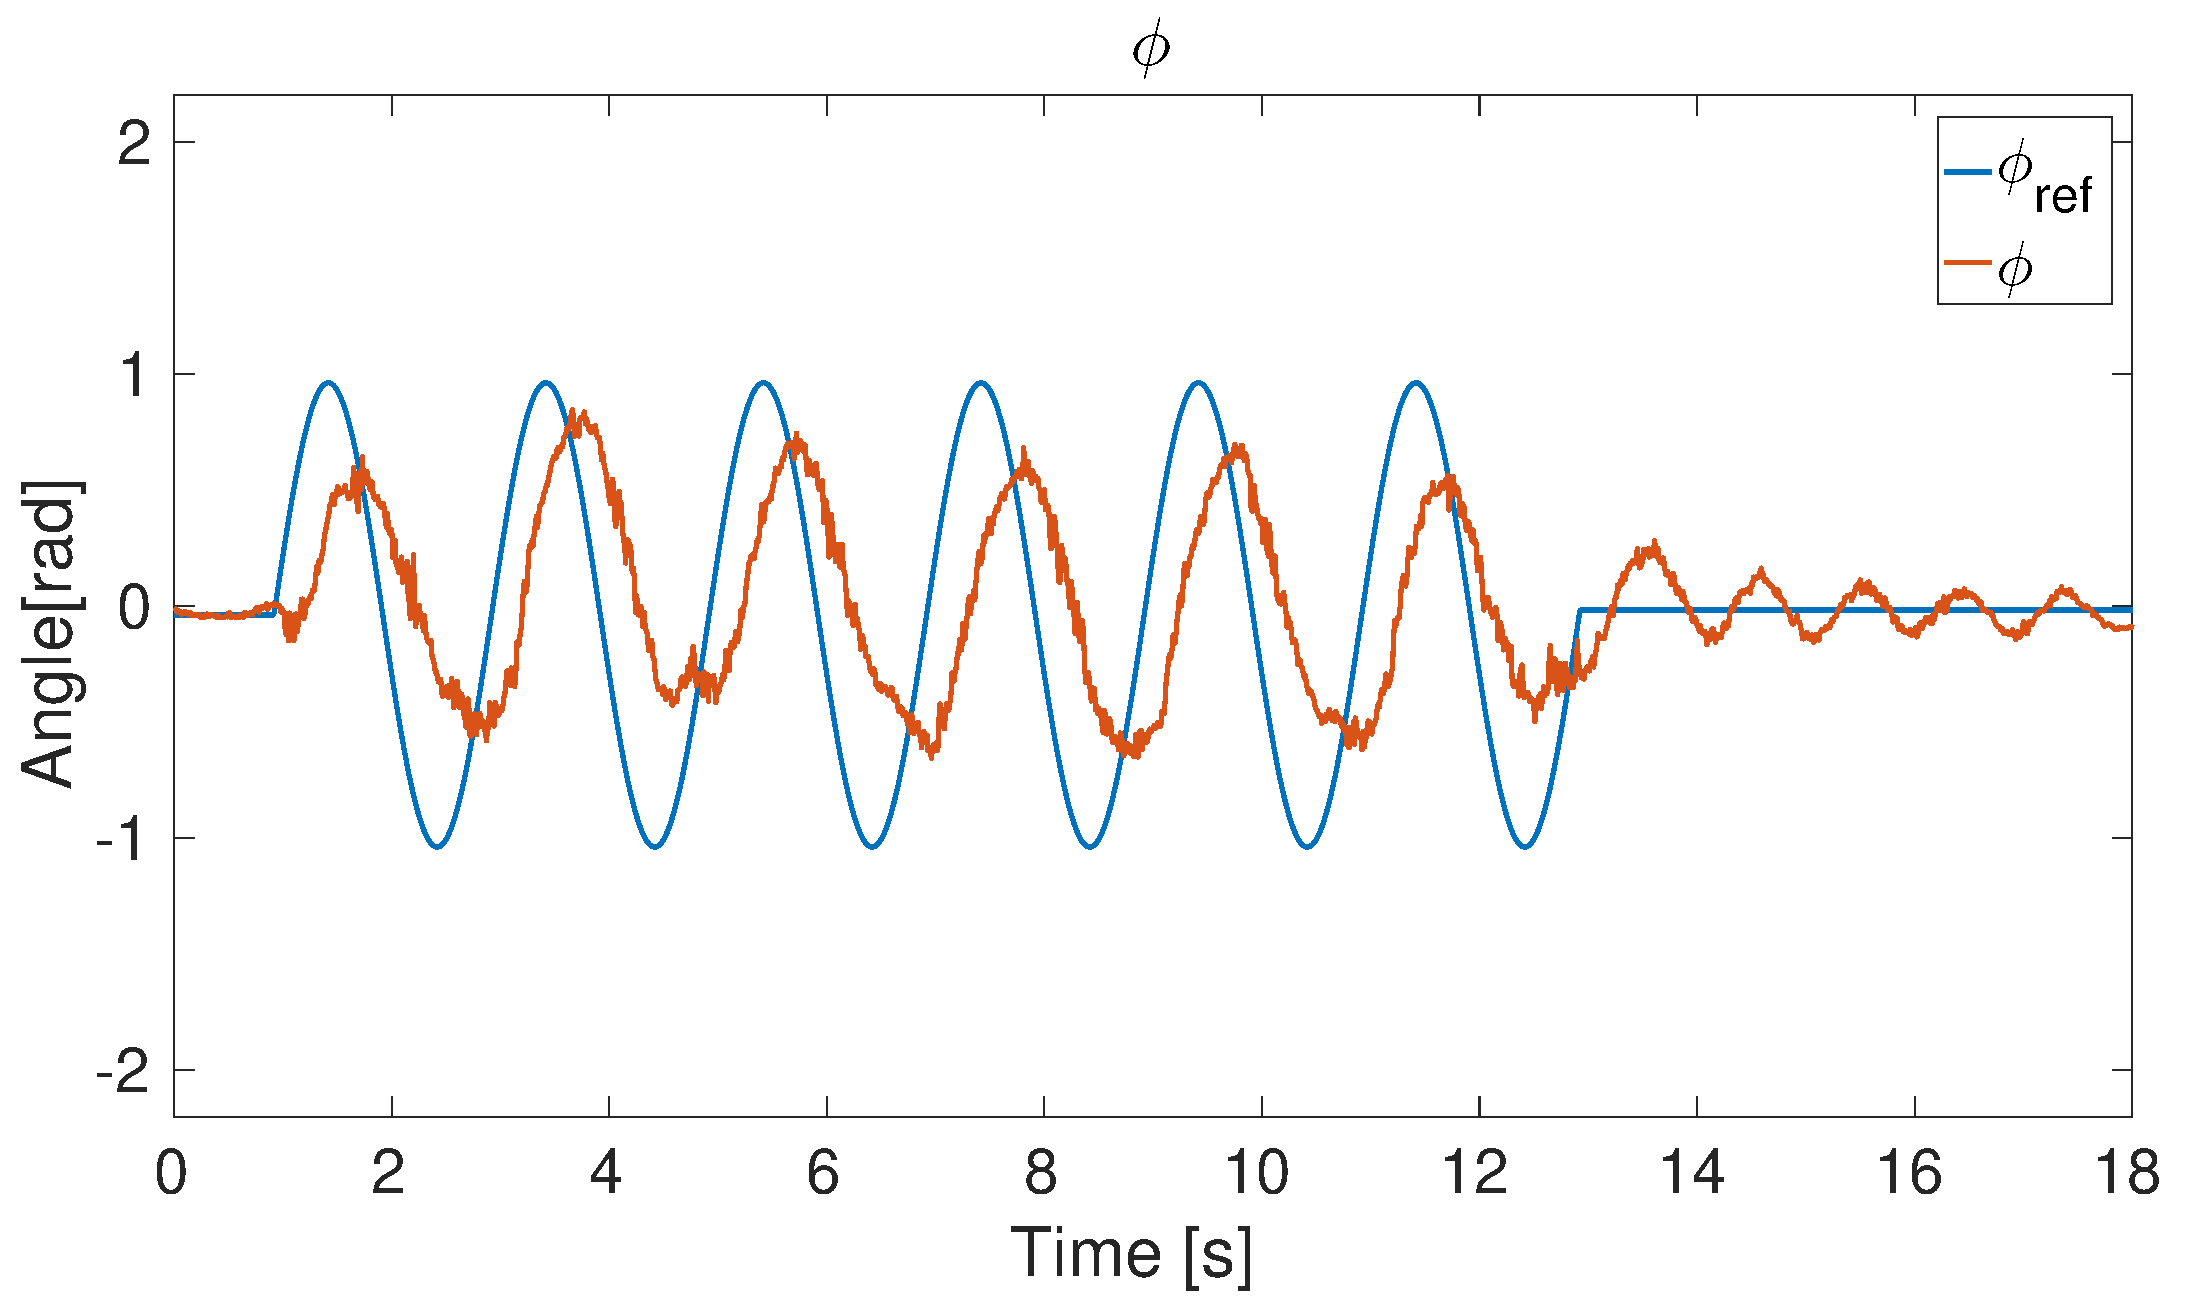
\includegraphics[width=0.4\textwidth]{testSinAllPhiA1}}
  \qquad
  \subfloat[][\label{fig:AppsimSinAllRollAttitude} A sine signal with amplitude $1$ and frequency $0.5\hertz$ applied to the simulated \abbrROV in $\rollAngle$.]{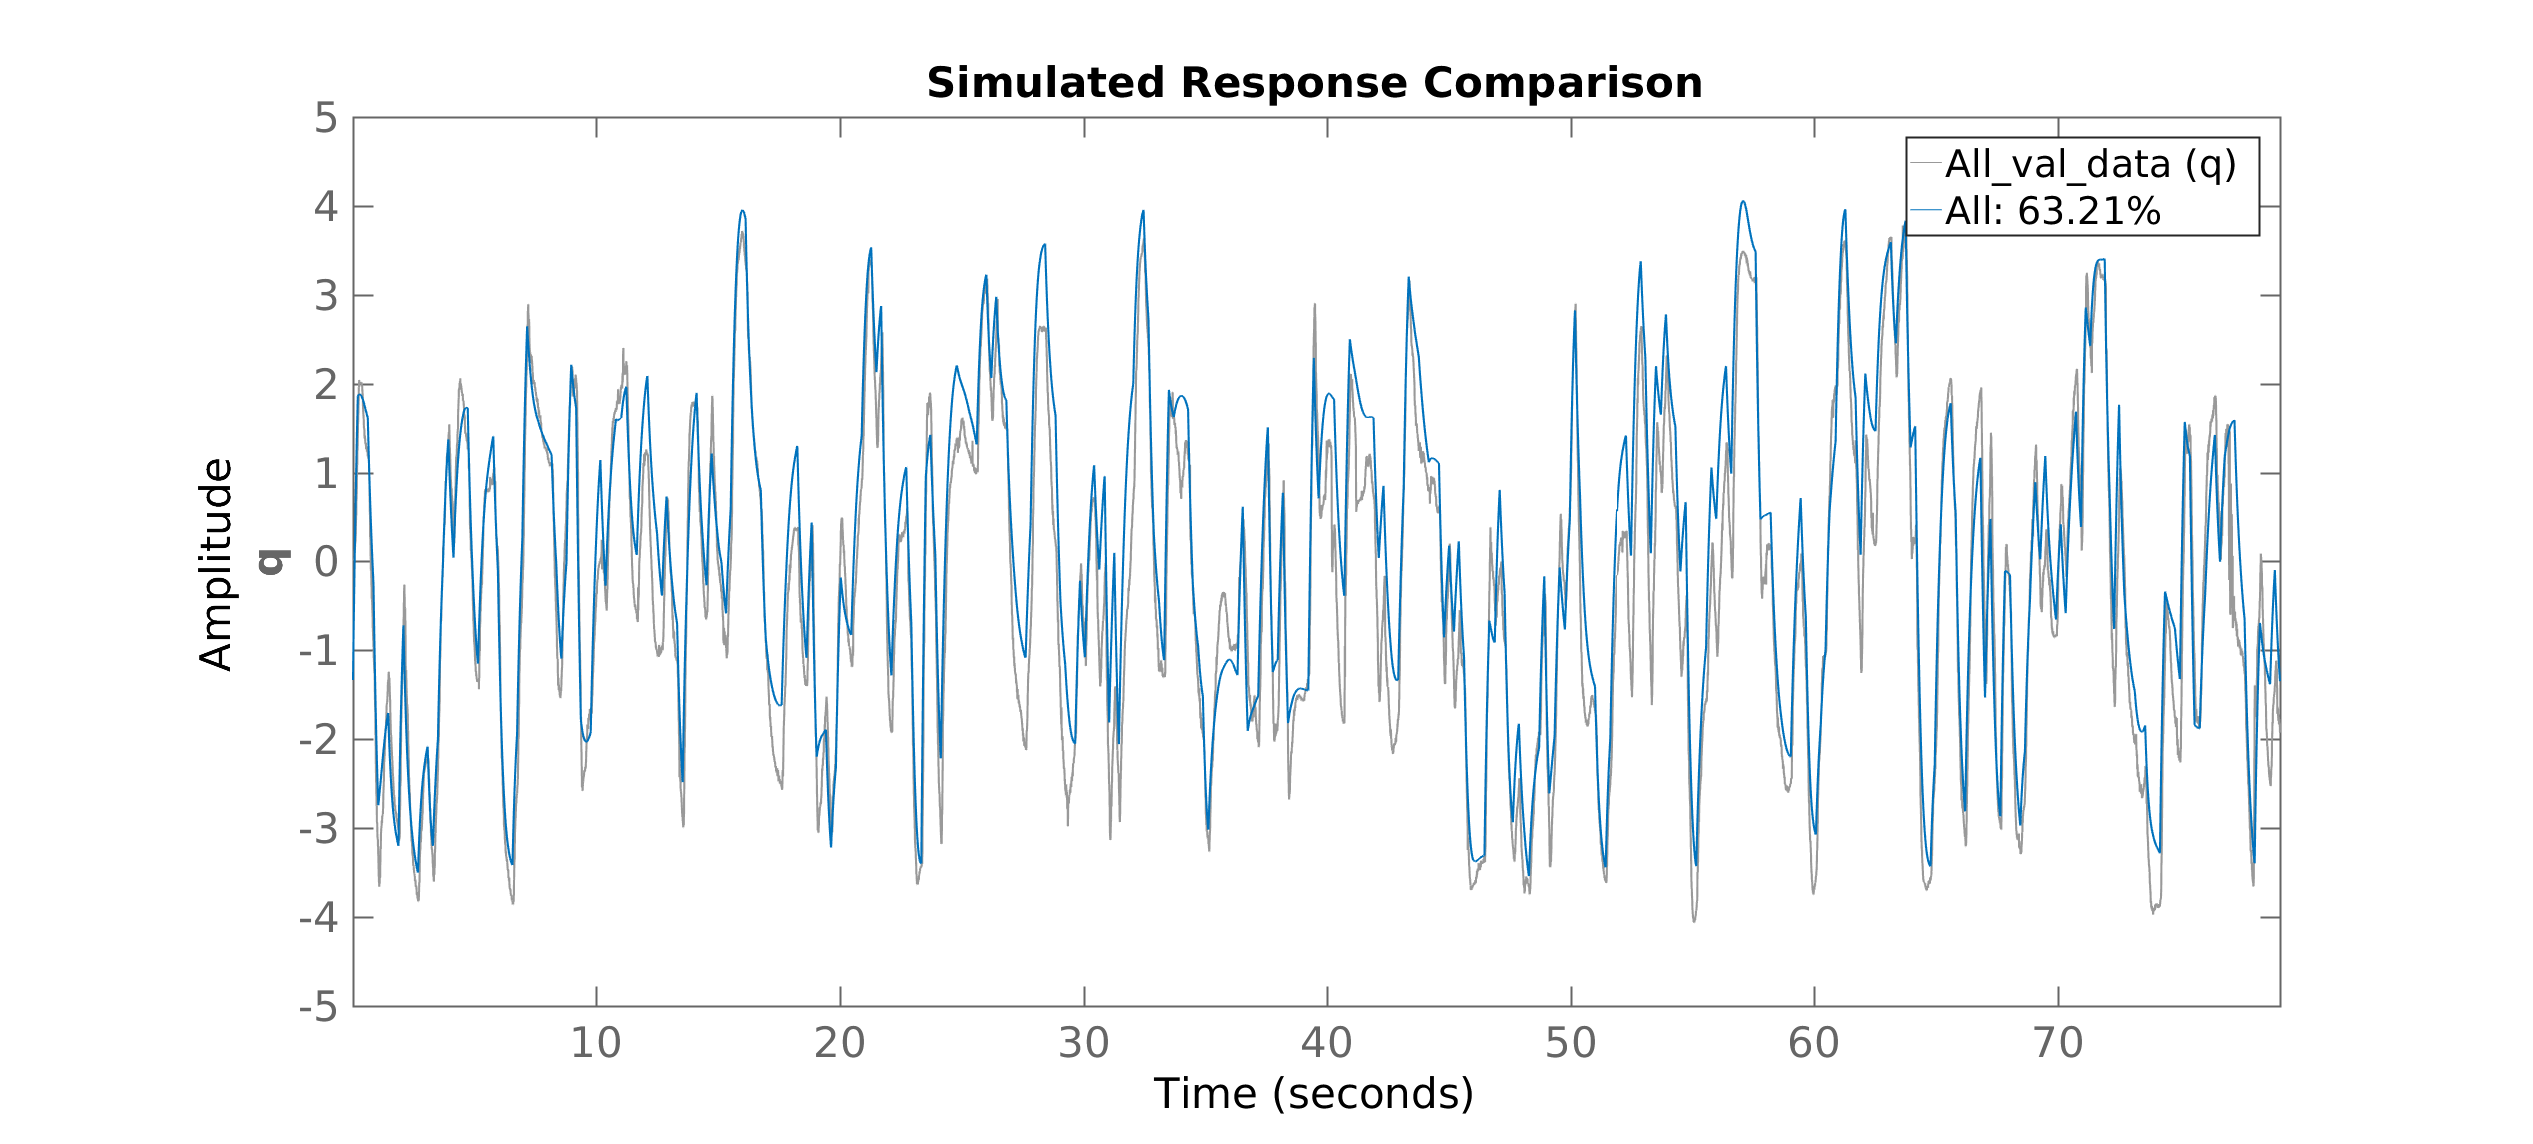
\includegraphics[width=0.4\textwidth]{velocityCompareq}}
  \qquad
  \subfloat[][\label{fig:ApptestSinAllPitchAttitude} A sine signal with amplitude $1$ and frequency $0.5\hertz$ applied in $\pitchAngle$.]{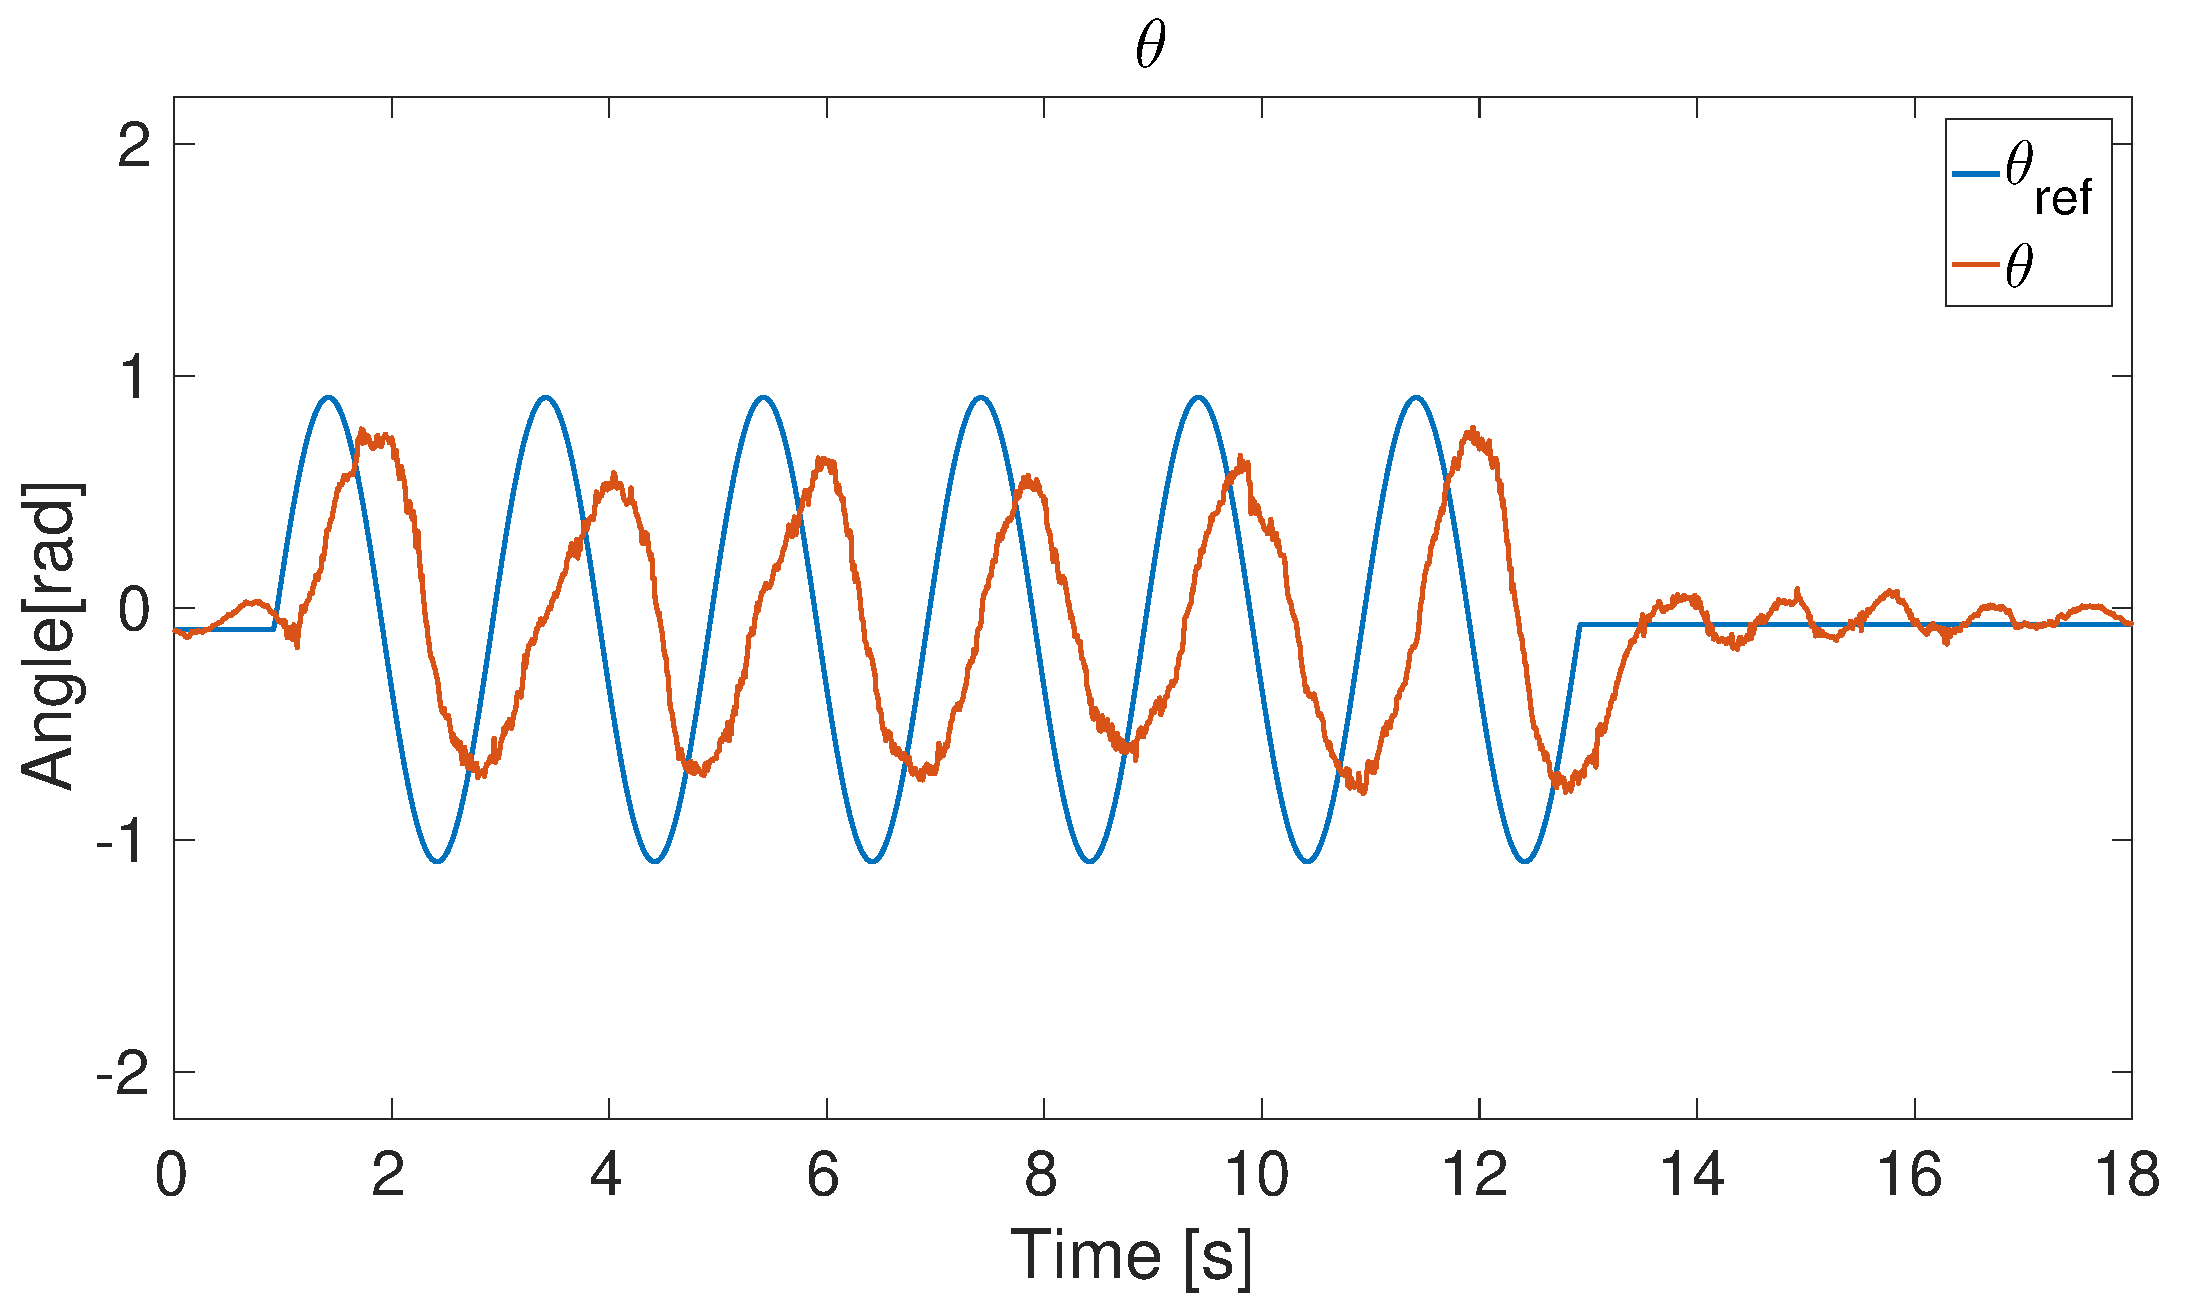
\includegraphics[width=0.4\textwidth]{testSinAllThetaA1}}
  \qquad
  \subfloat[][\label{fig:AppsimSinAllPitchAttitude} A sine signal with amplitude $1$ and frequency $0.5\hertz$ applied to the simulated \abbrROV in $\pitchAngle$.]{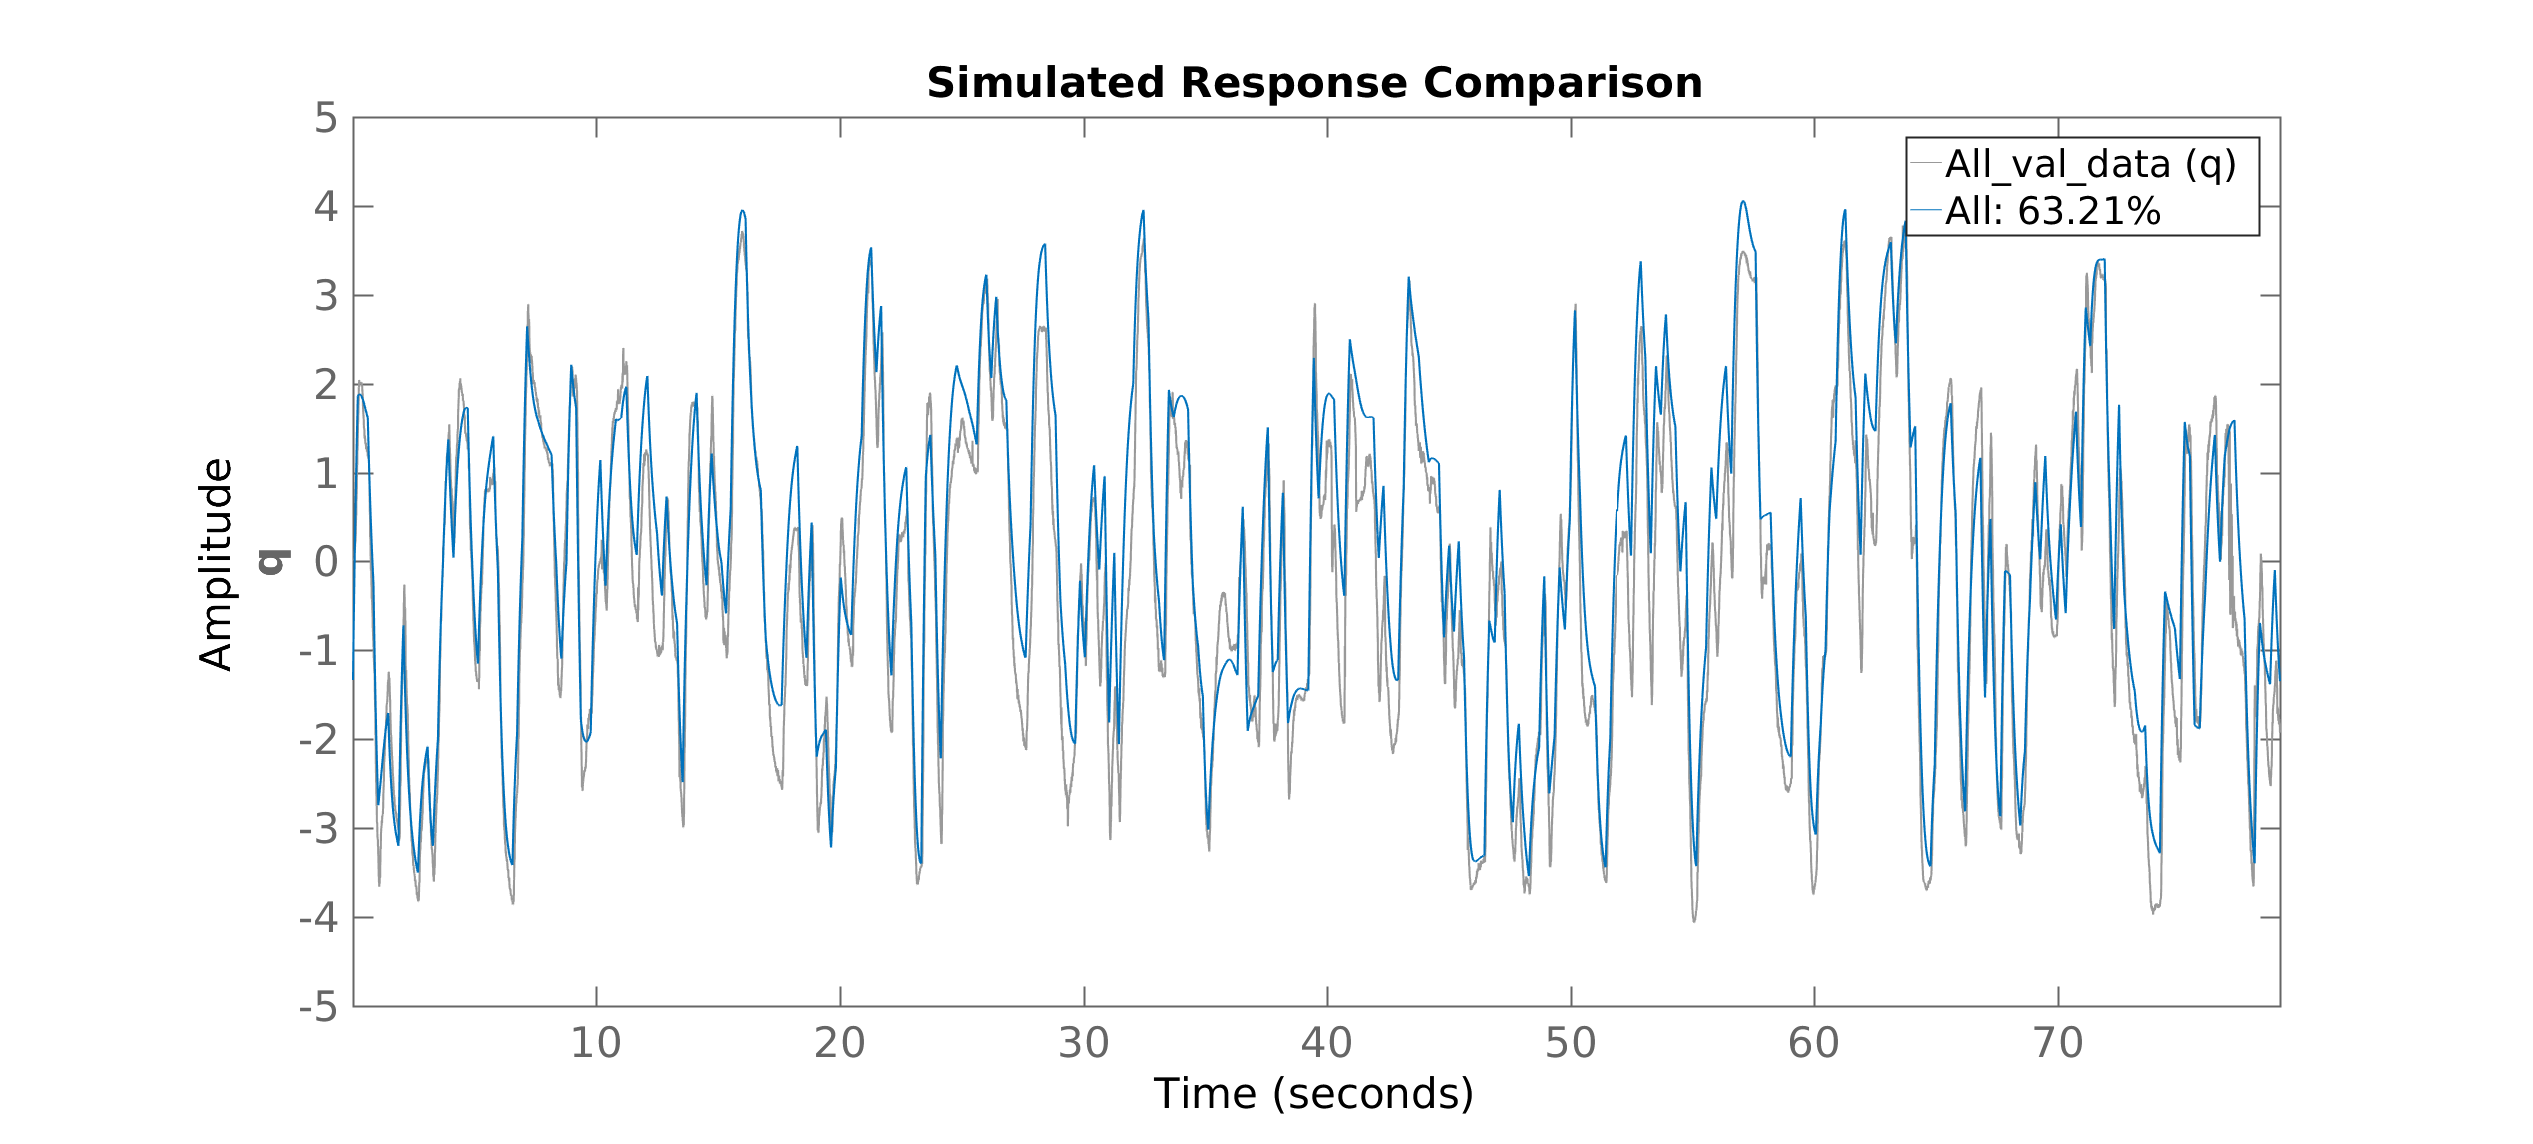
\includegraphics[width=0.4\textwidth]{velocityCompareq}}
  \qquad
  \subfloat[][\label{fig:ApptestSinAllYawAttitude} A sine signal with amplitude $1$ and frequency $0.5\hertz$ applied in $\yawAngle$.]{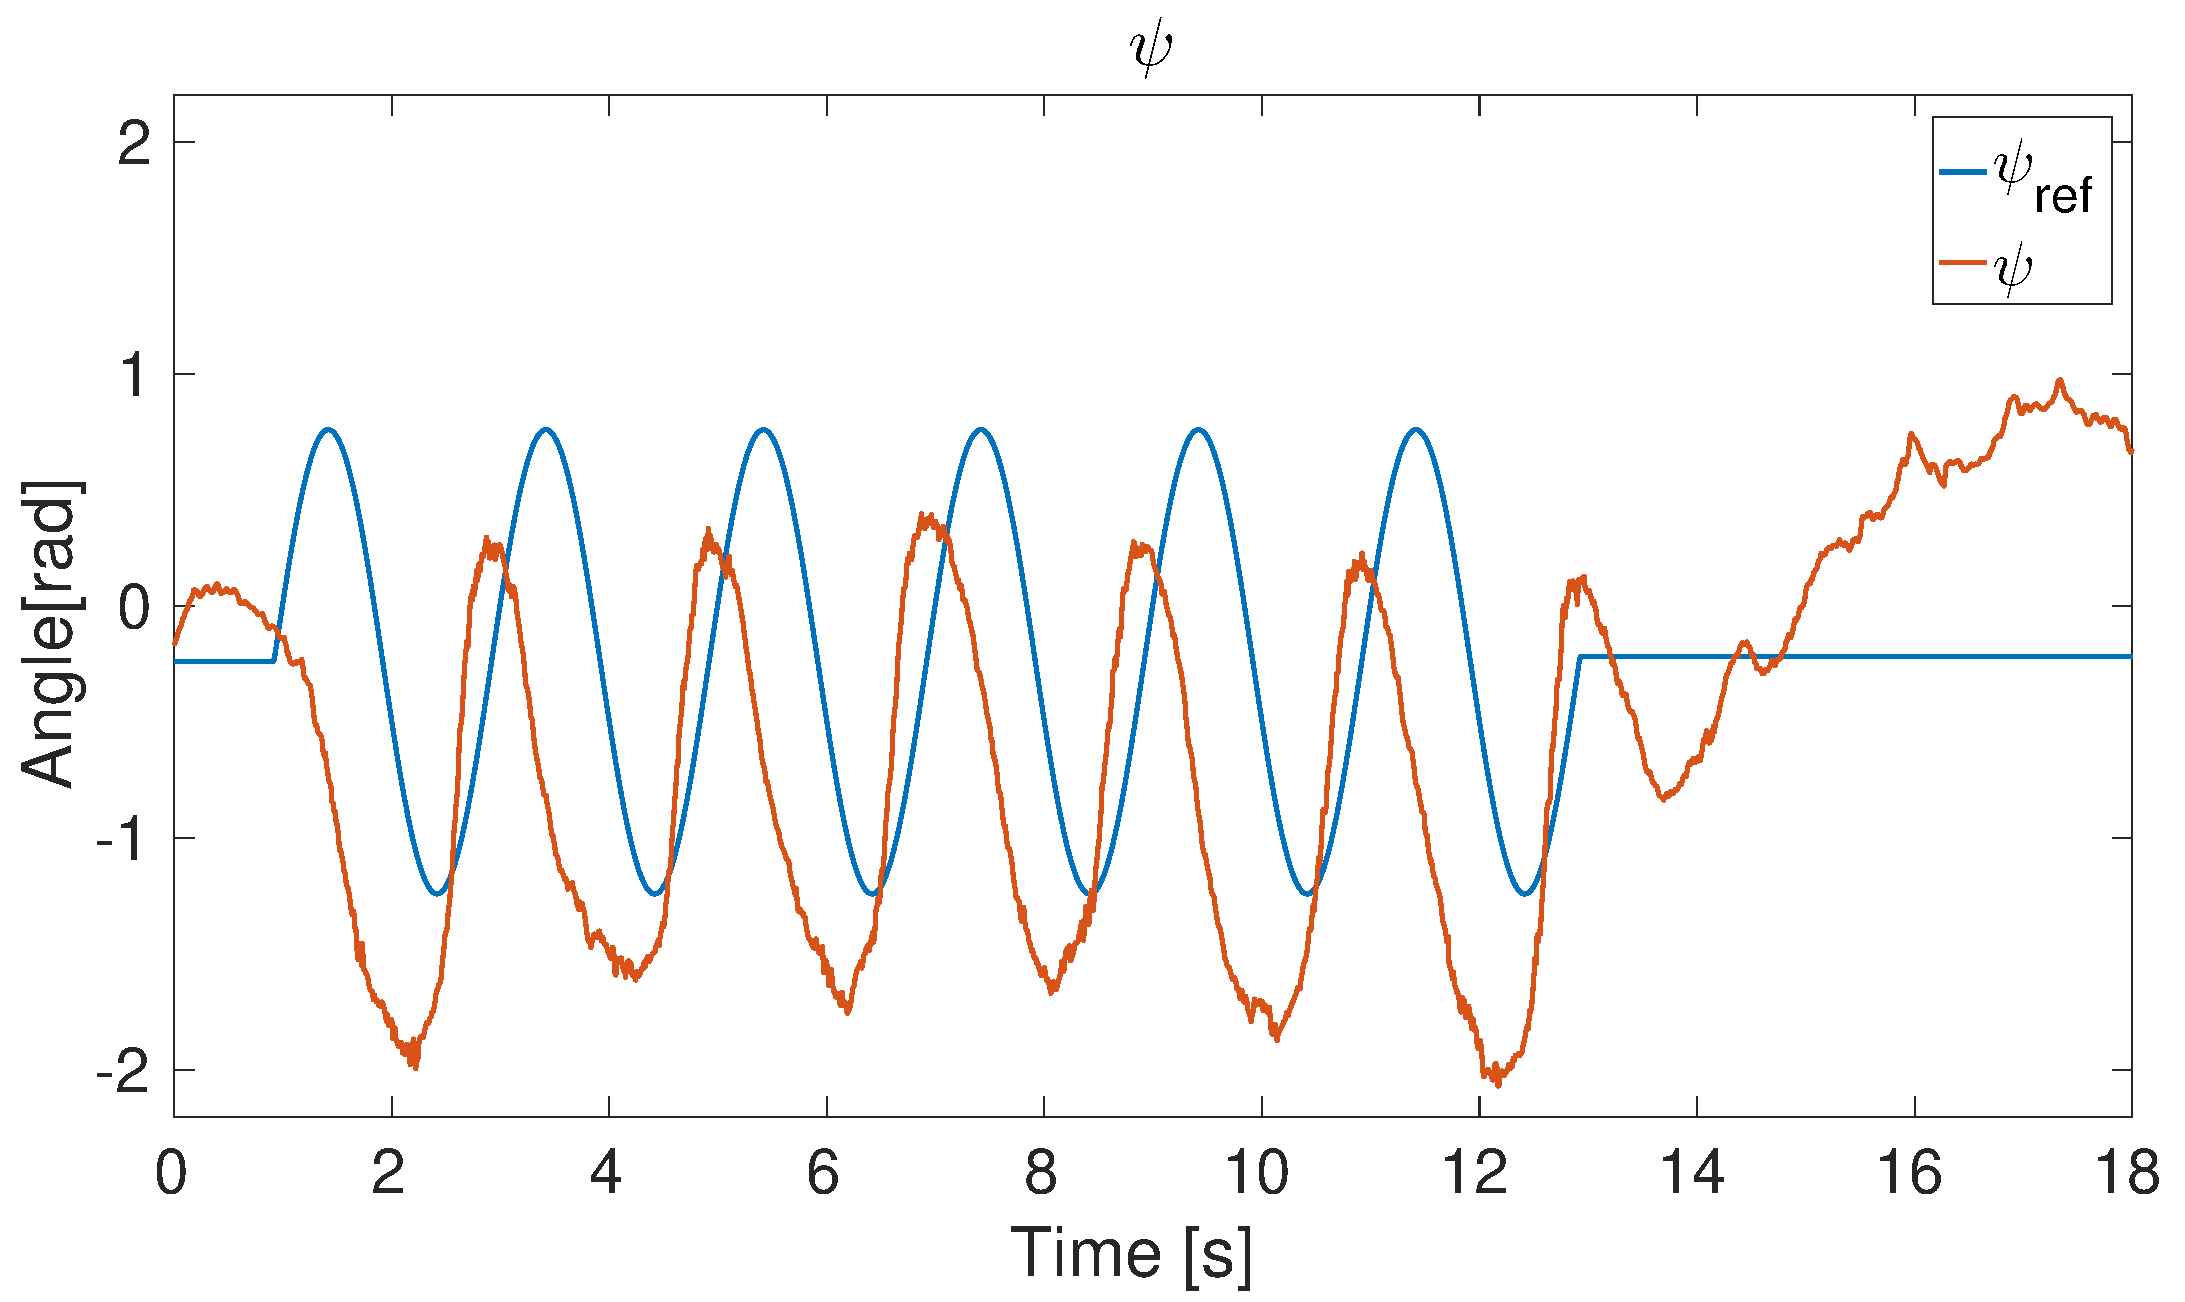
\includegraphics[width=0.4\textwidth]{testSinAllPsiA1}}
  \qquad
  \subfloat[][\label{fig:AppsimSinAllYawAttitude} A sine signal with amplitude $1$ and frequency $0.5\hertz$ applied to the simulated \abbrROV in $\yawAngle$.]{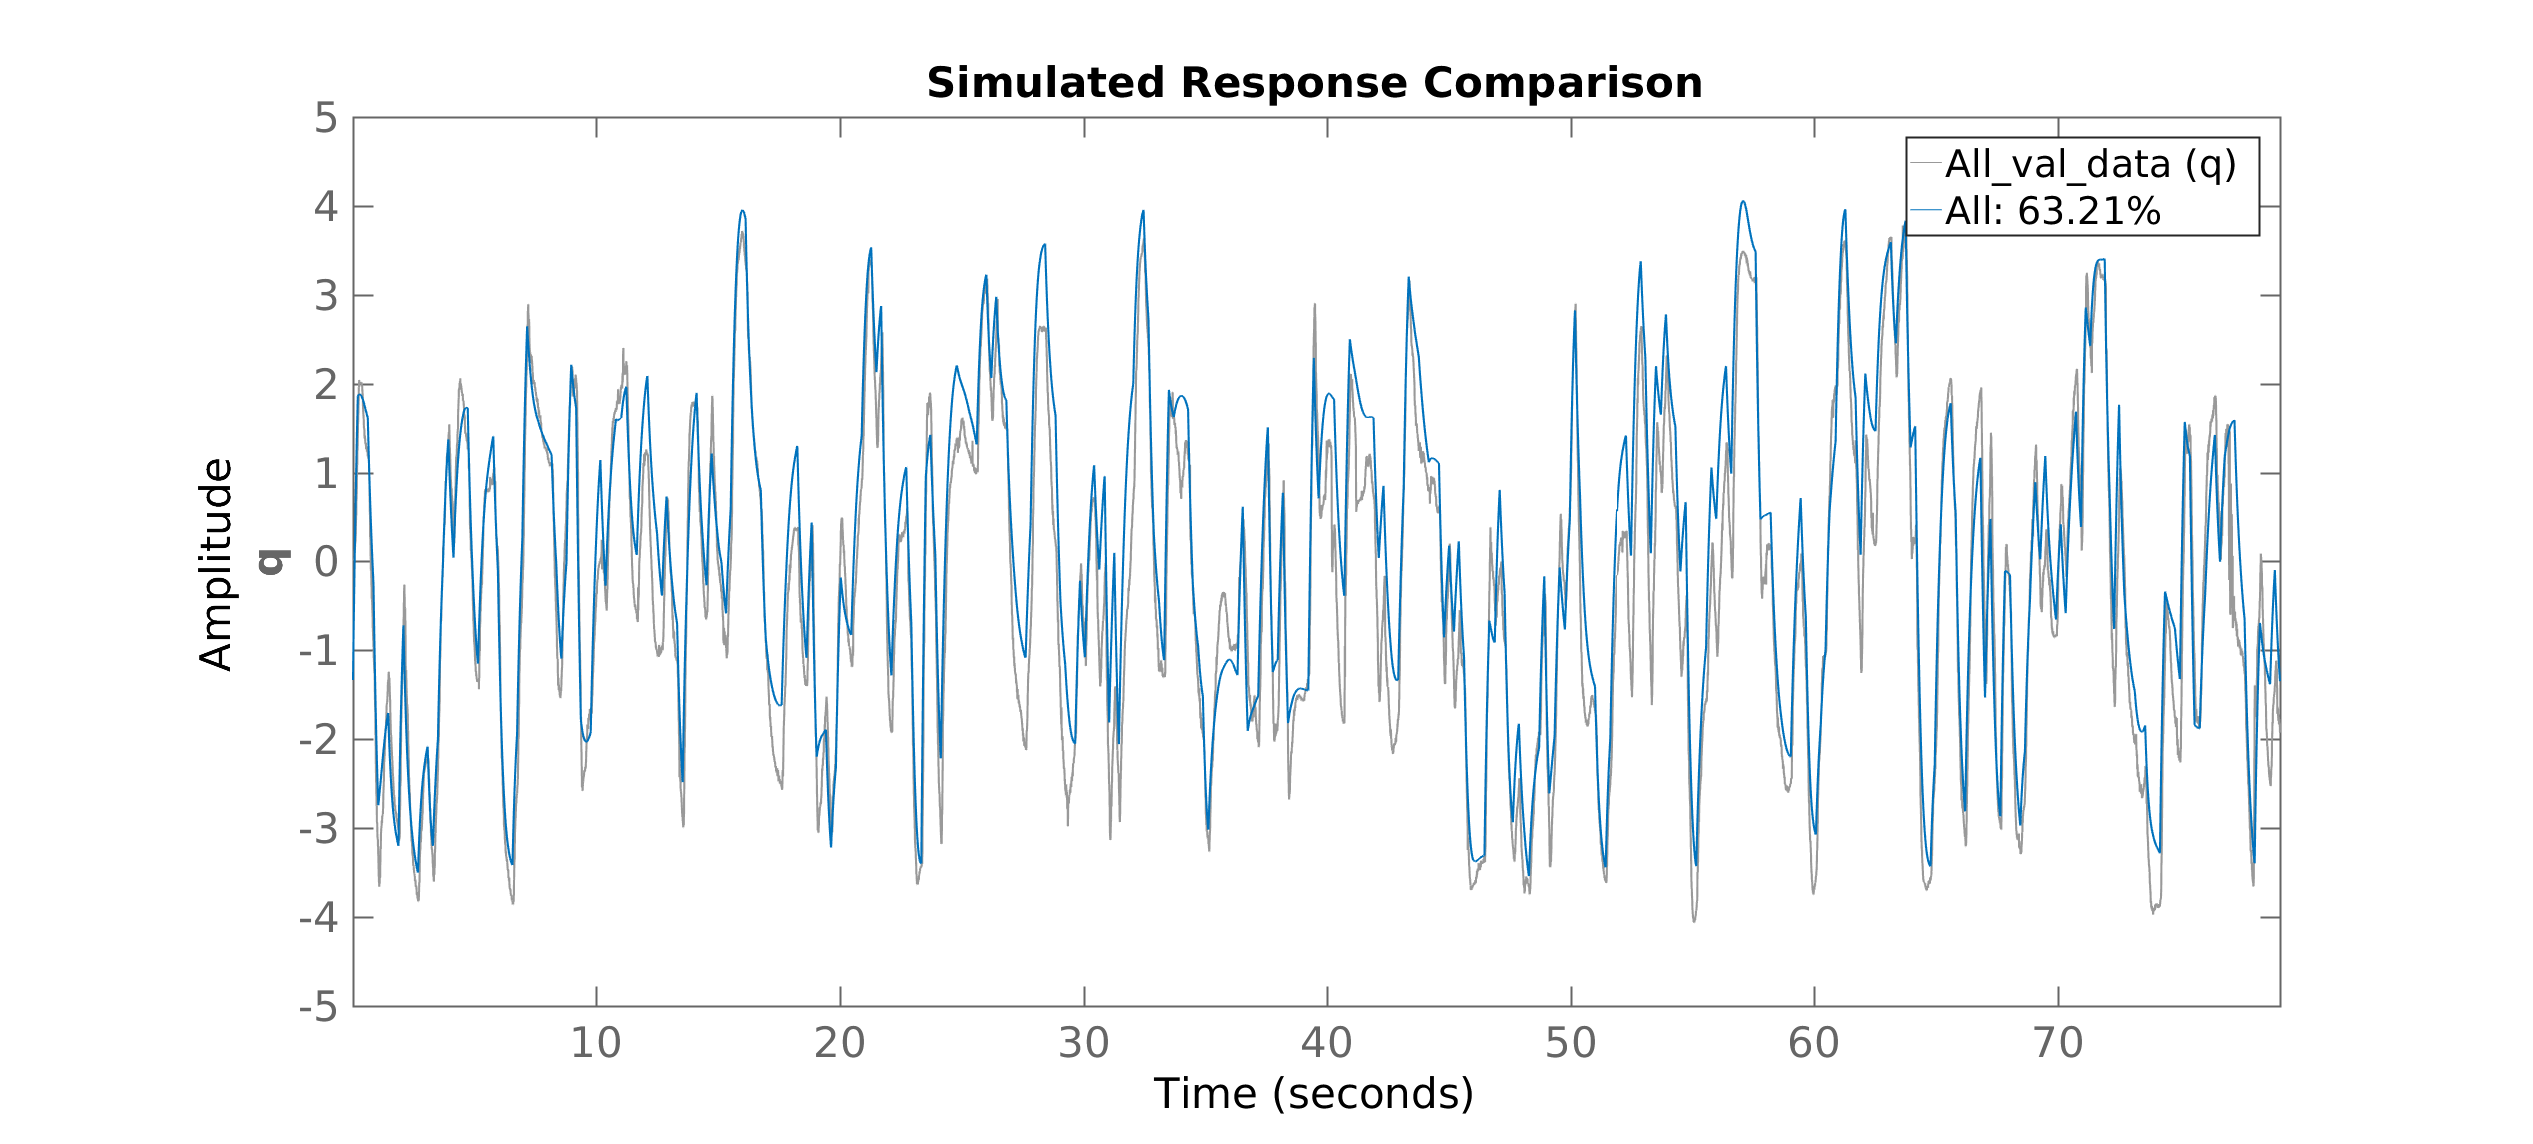
\includegraphics[width=0.4\textwidth]{velocityCompareq}}
  \caption{\label{fig:AppSinAllAttitude}%
  Sine signals were applied in all attitude angles at the same time while using the attitude controller.}
\end{figure}


\begin{figure}[tbp]
  \centering
  \subfloat[][\label{fig:ApptestSin05Roll} A sine signal with amplitude $0.5$ and frequency $0.5\hertz$ applied in $\rollAngle$.]{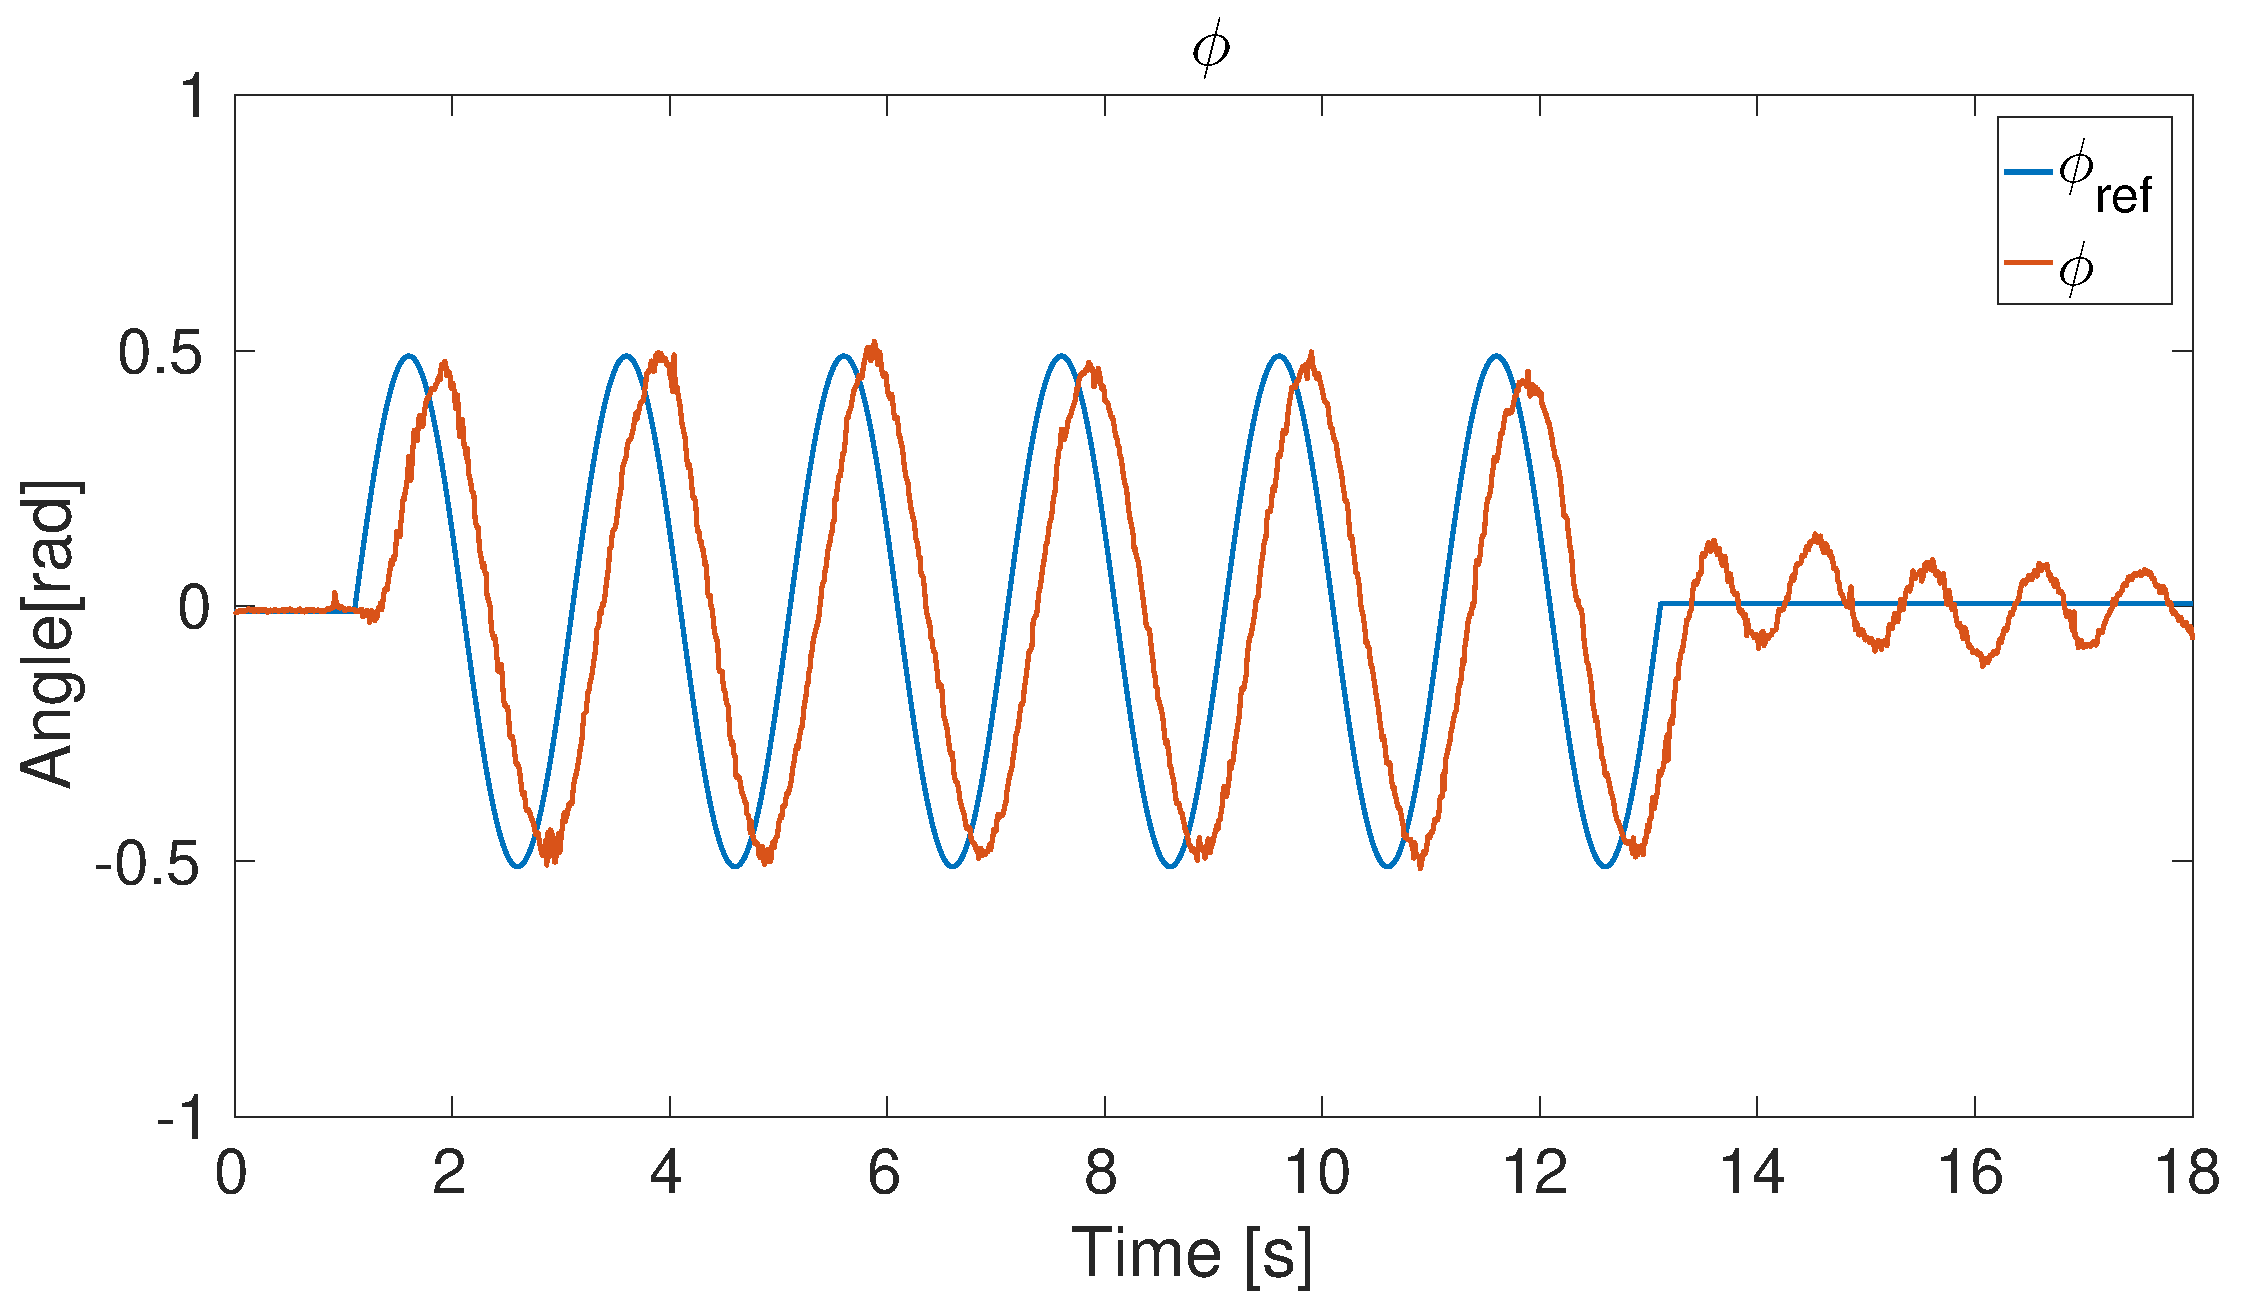
\includegraphics[width=0.4\textwidth]{testSinPhiA05}}
  \qquad
  \subfloat[][\label{fig:AppsimSin05Roll} A sine signal with amplitude $0.5$ and frequency $0.5\hertz$ applied to the simulated \abbrROV in $\rollAngle$.]{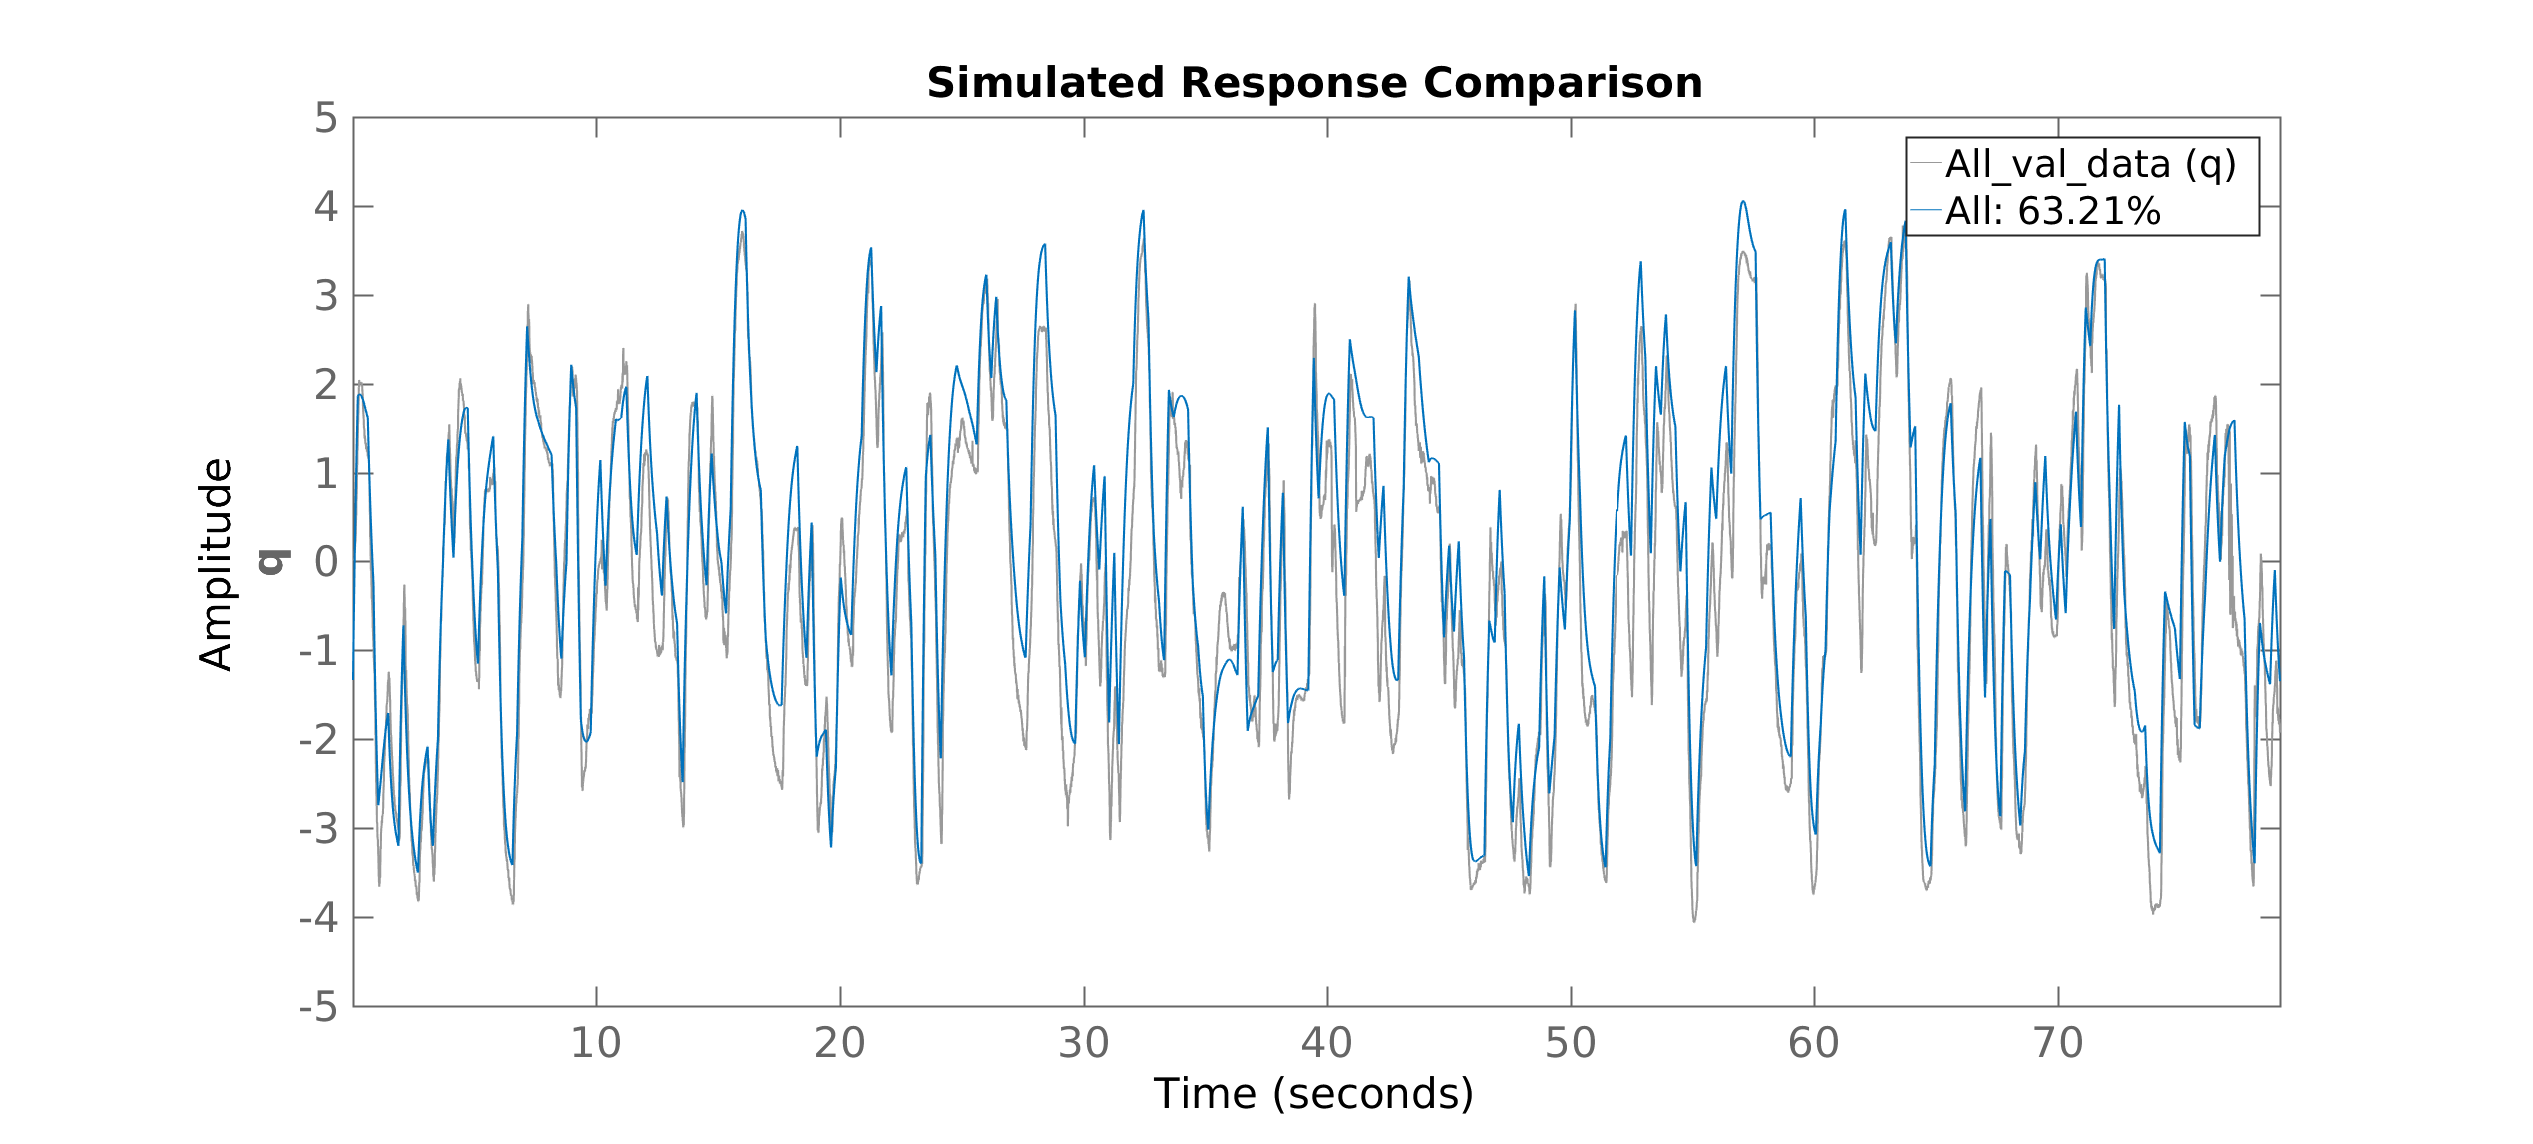
\includegraphics[width=0.4\textwidth]{velocityCompareq}}
  \qquad
  \subfloat[][\label{fig:ApptestSin05Pitch} A sine signal with amplitude $0.5$ and frequency $0.5\hertz$ applied in $\pitchAngle$.]{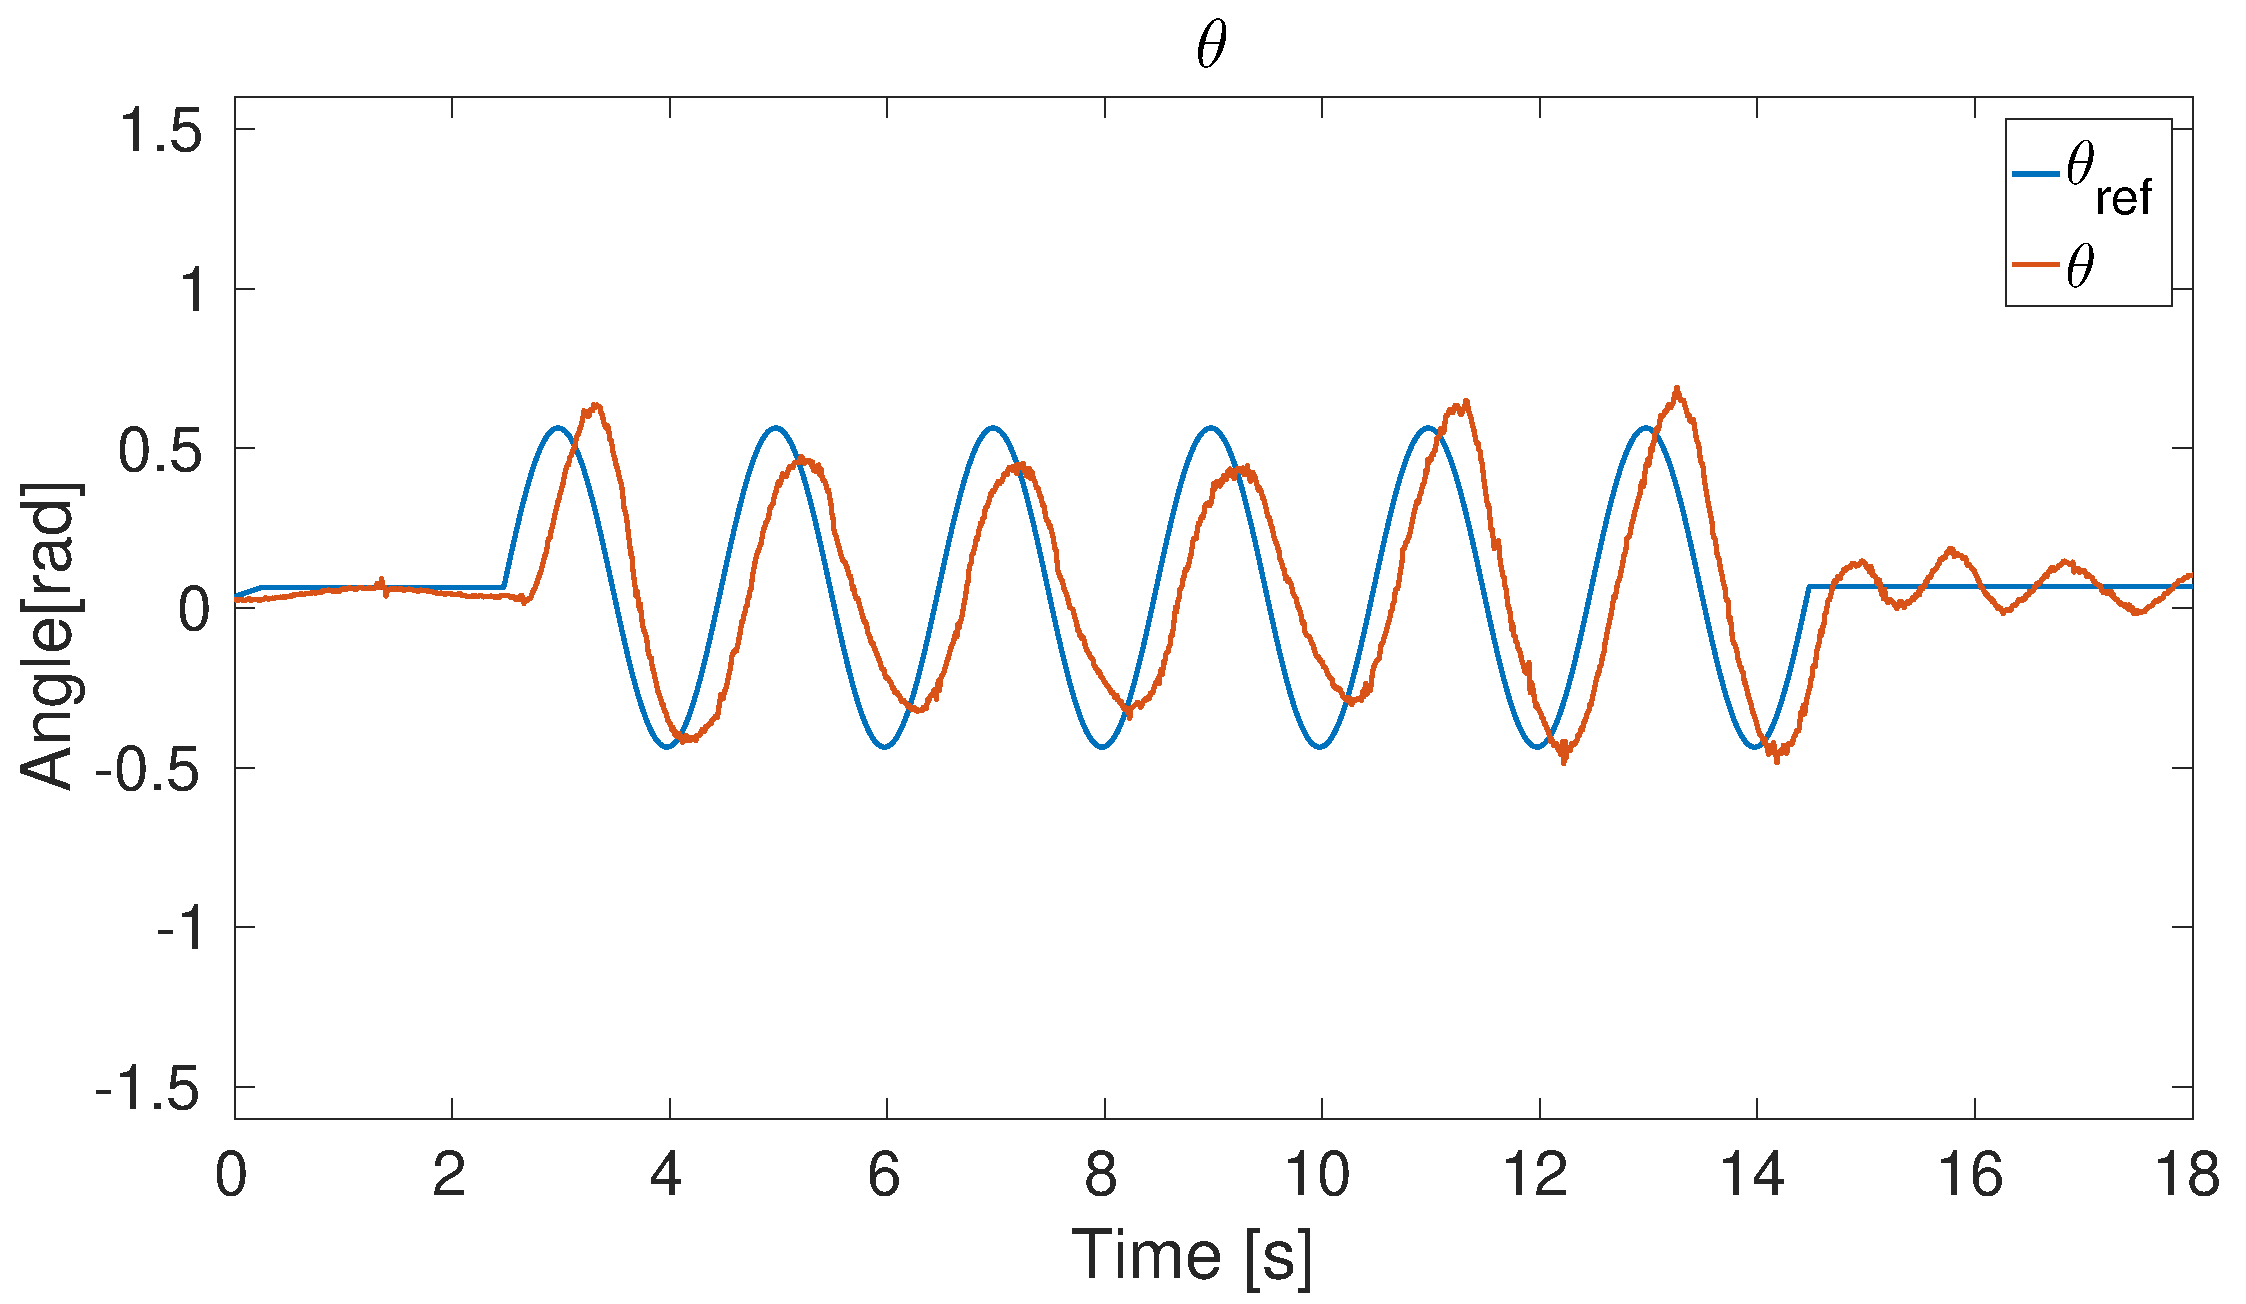
\includegraphics[width=0.4\textwidth]{testSinThetaA05}}
  \qquad
  \subfloat[][\label{fig:AppsimSin05Pitch} A sine signal with amplitude $0.5$ and frequency $0.5\hertz$ applied to the simulated \abbrROV in $\pitchAngle$.]{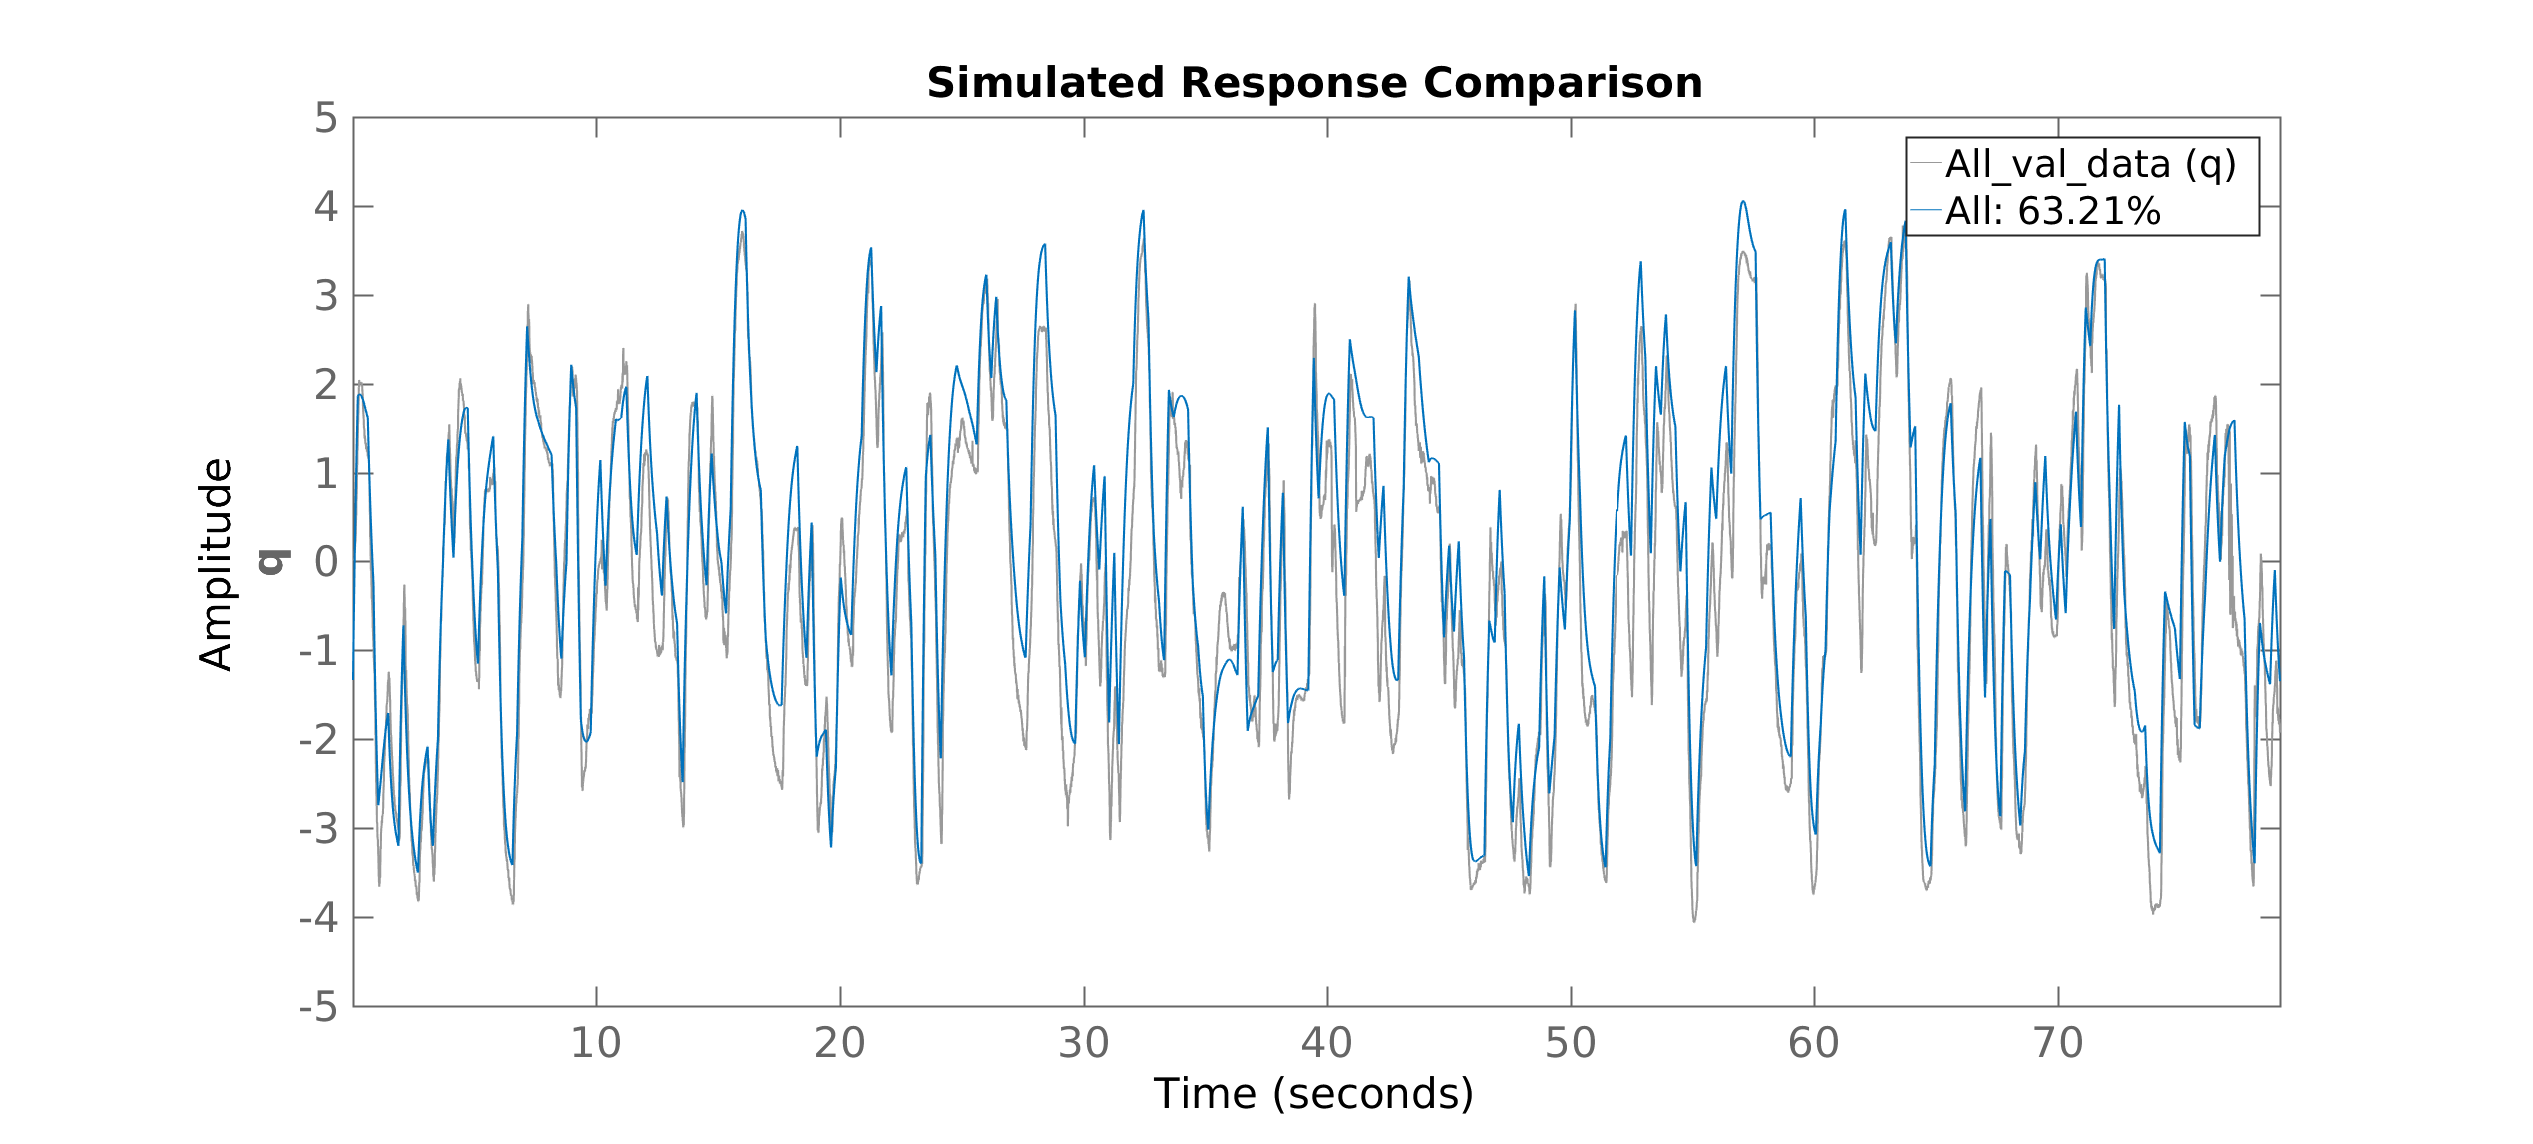
\includegraphics[width=0.4\textwidth]{velocityCompareq}}
  \qquad
  \subfloat[][\label{fig:ApptestSin05Yaw} A sine signal with amplitude $0.5$ and frequency $0.5\hertz$ applied in $\yawAngle$.]{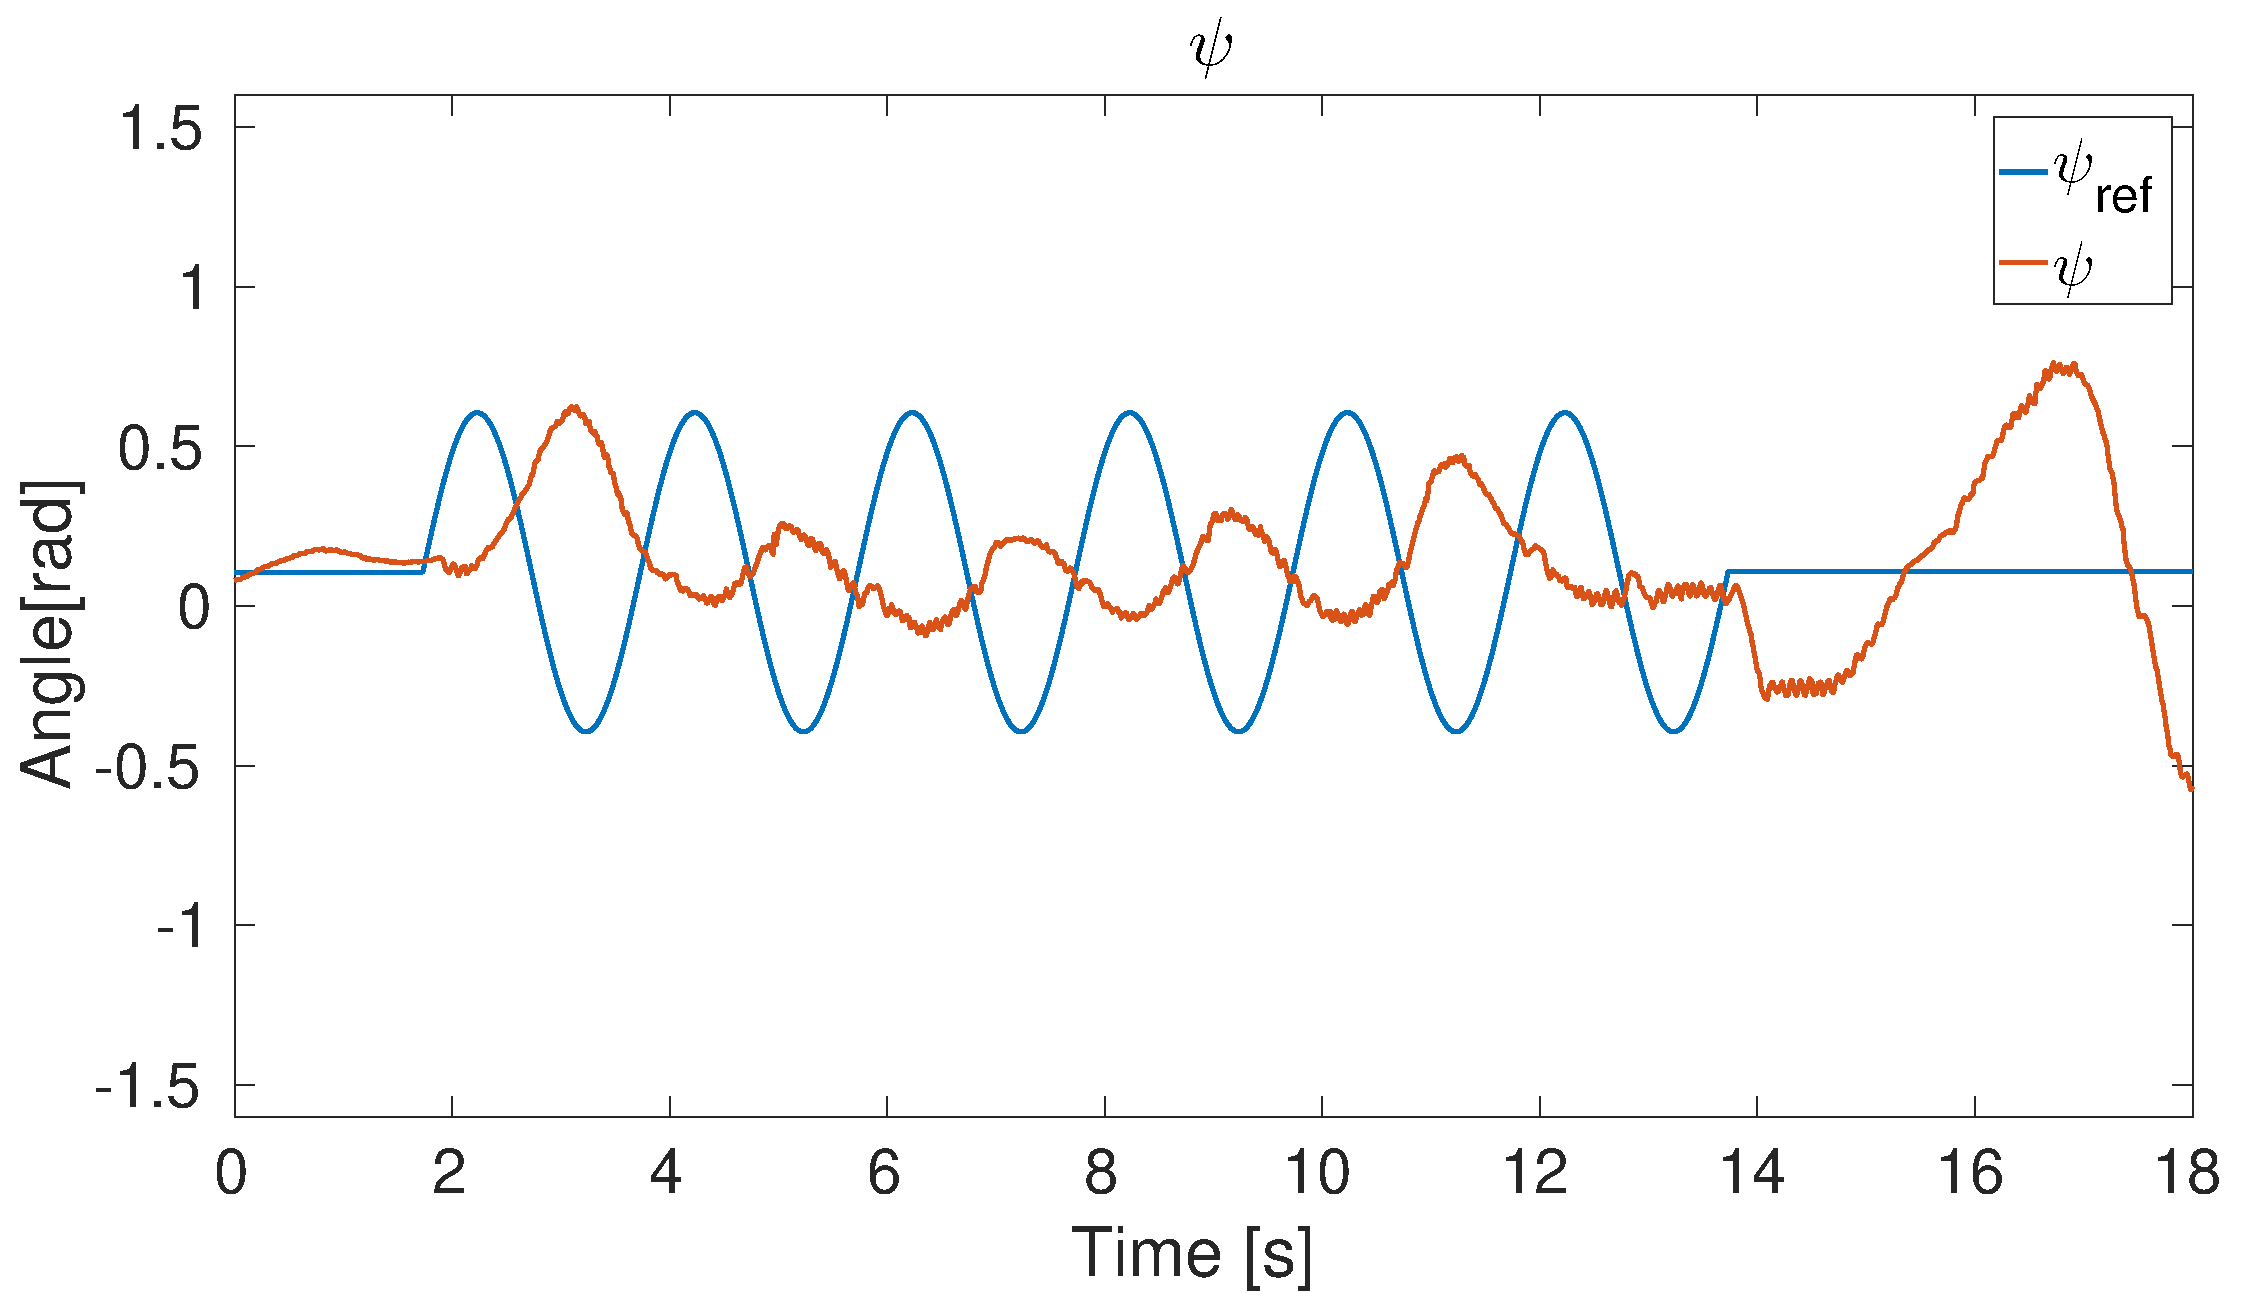
\includegraphics[width=0.4\textwidth]{testSinPsiA05}}
  \qquad
  \subfloat[][\label{fig:AppsimSin50Yaw} A sine signal with amplitude $0.5$ and frequency $0.5\hertz$ applied to the simulated \abbrROV in $\yawAngle$.]{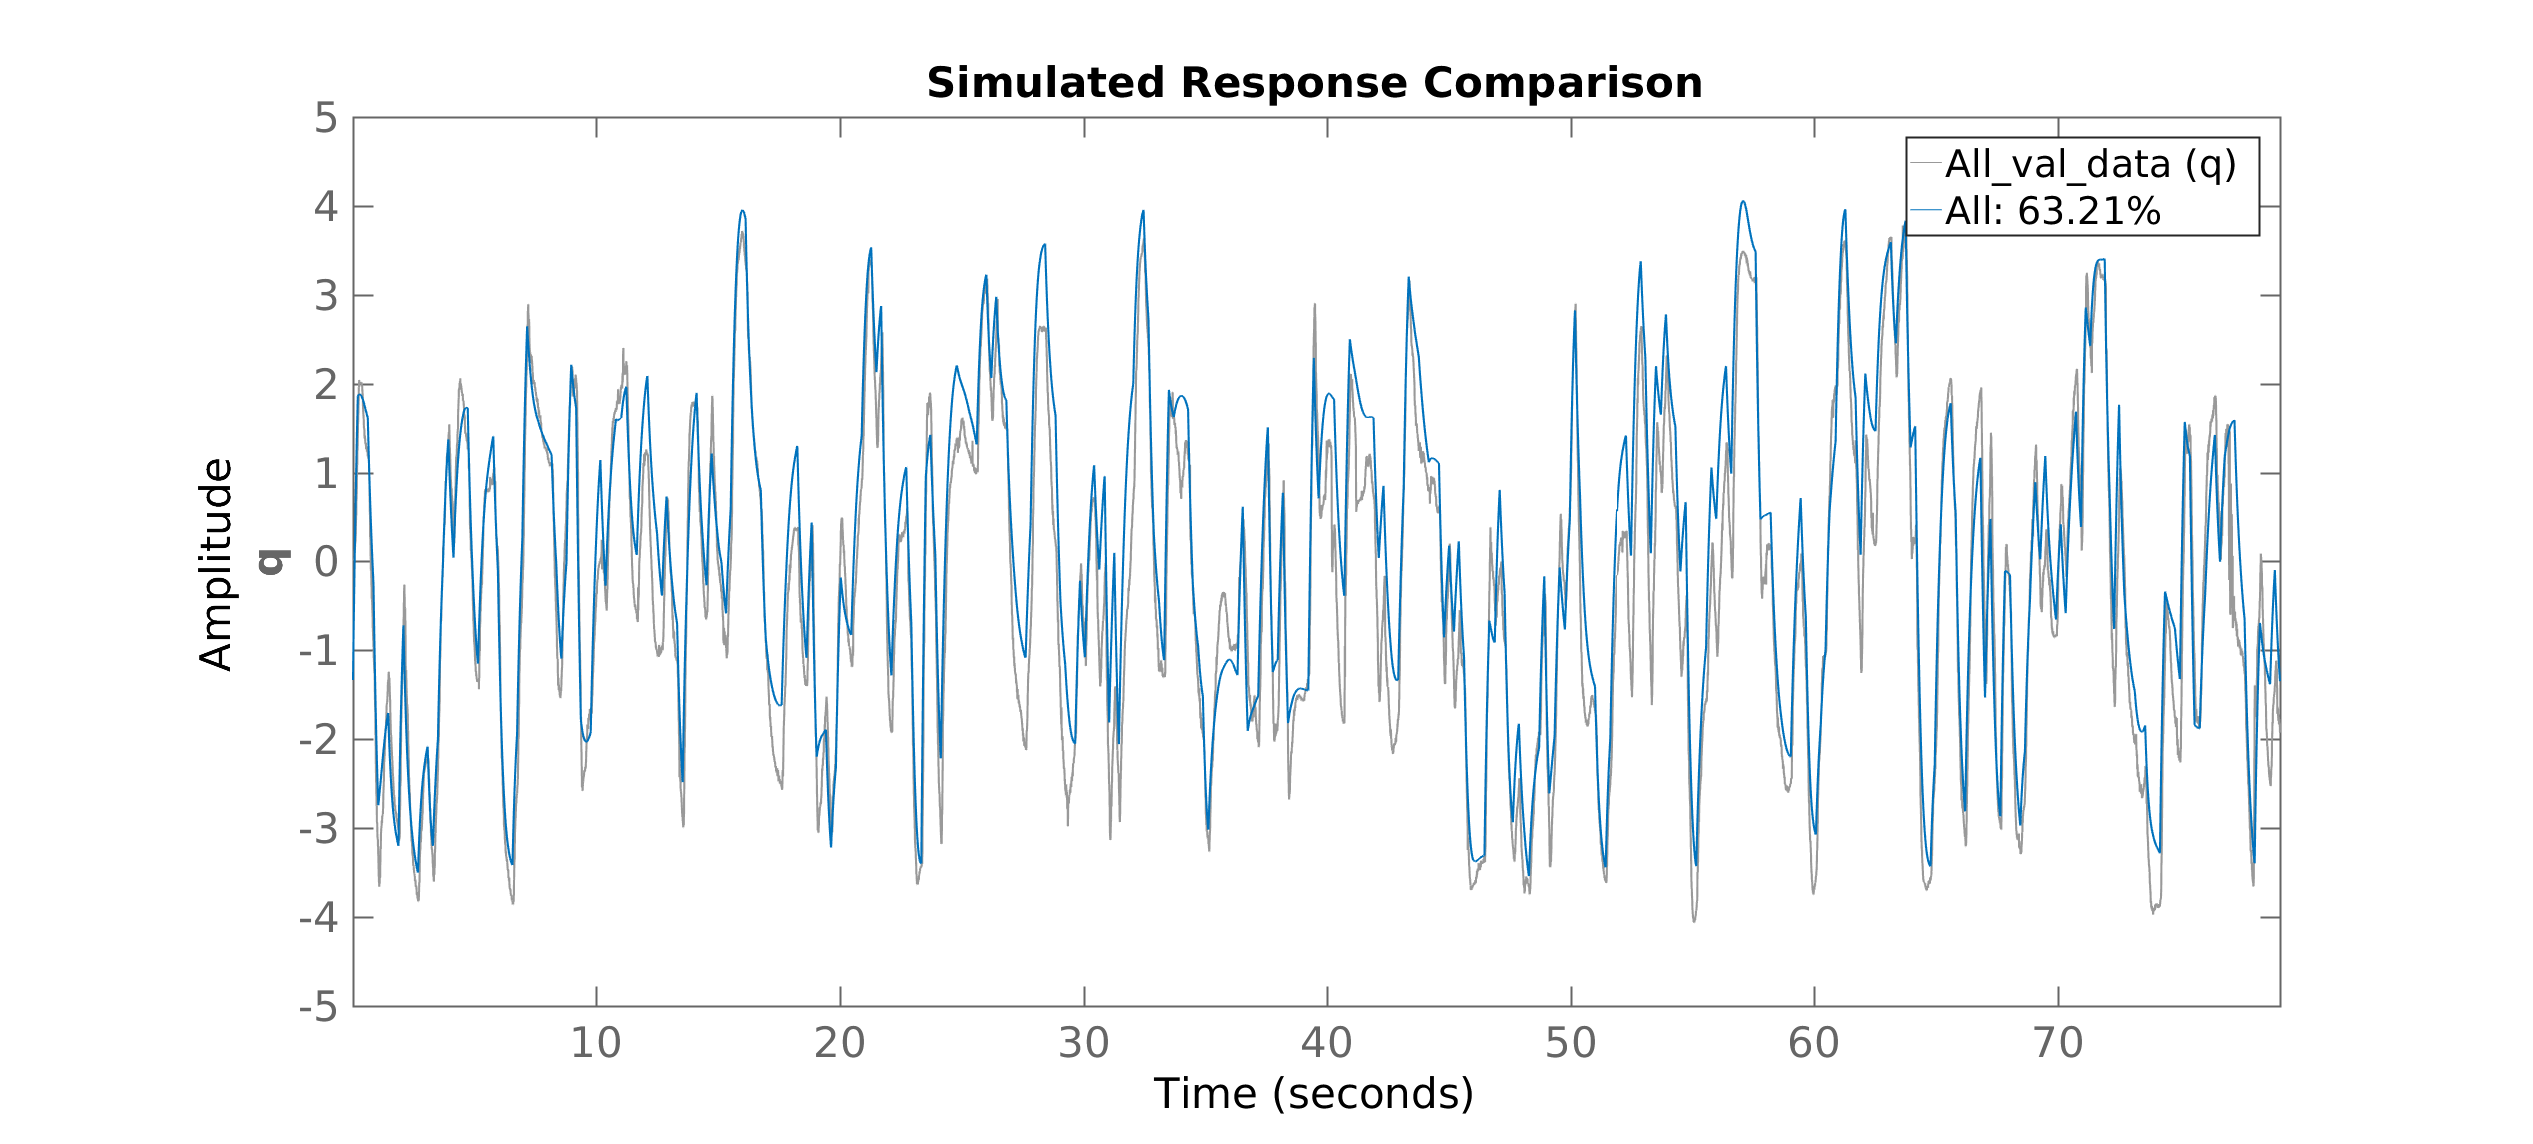
\includegraphics[width=0.4\textwidth]{velocityCompareq}}
    \caption{\label{fig:AppSin05Attitude}%
   A sine signal was applied in one attitude angle at a time while using the attitude controller. While a sine signal was applied in one attitude angle the other attitude angles were not controlled.}
\end{figure}

\begin{figure}
\centering
  \subfloat[][\label{fig:ApptestSinAll05RollAttitude} A sine signal with amplitude $0.5$ and frequency $0.5\hertz$ applied in $\rollAngle$.]{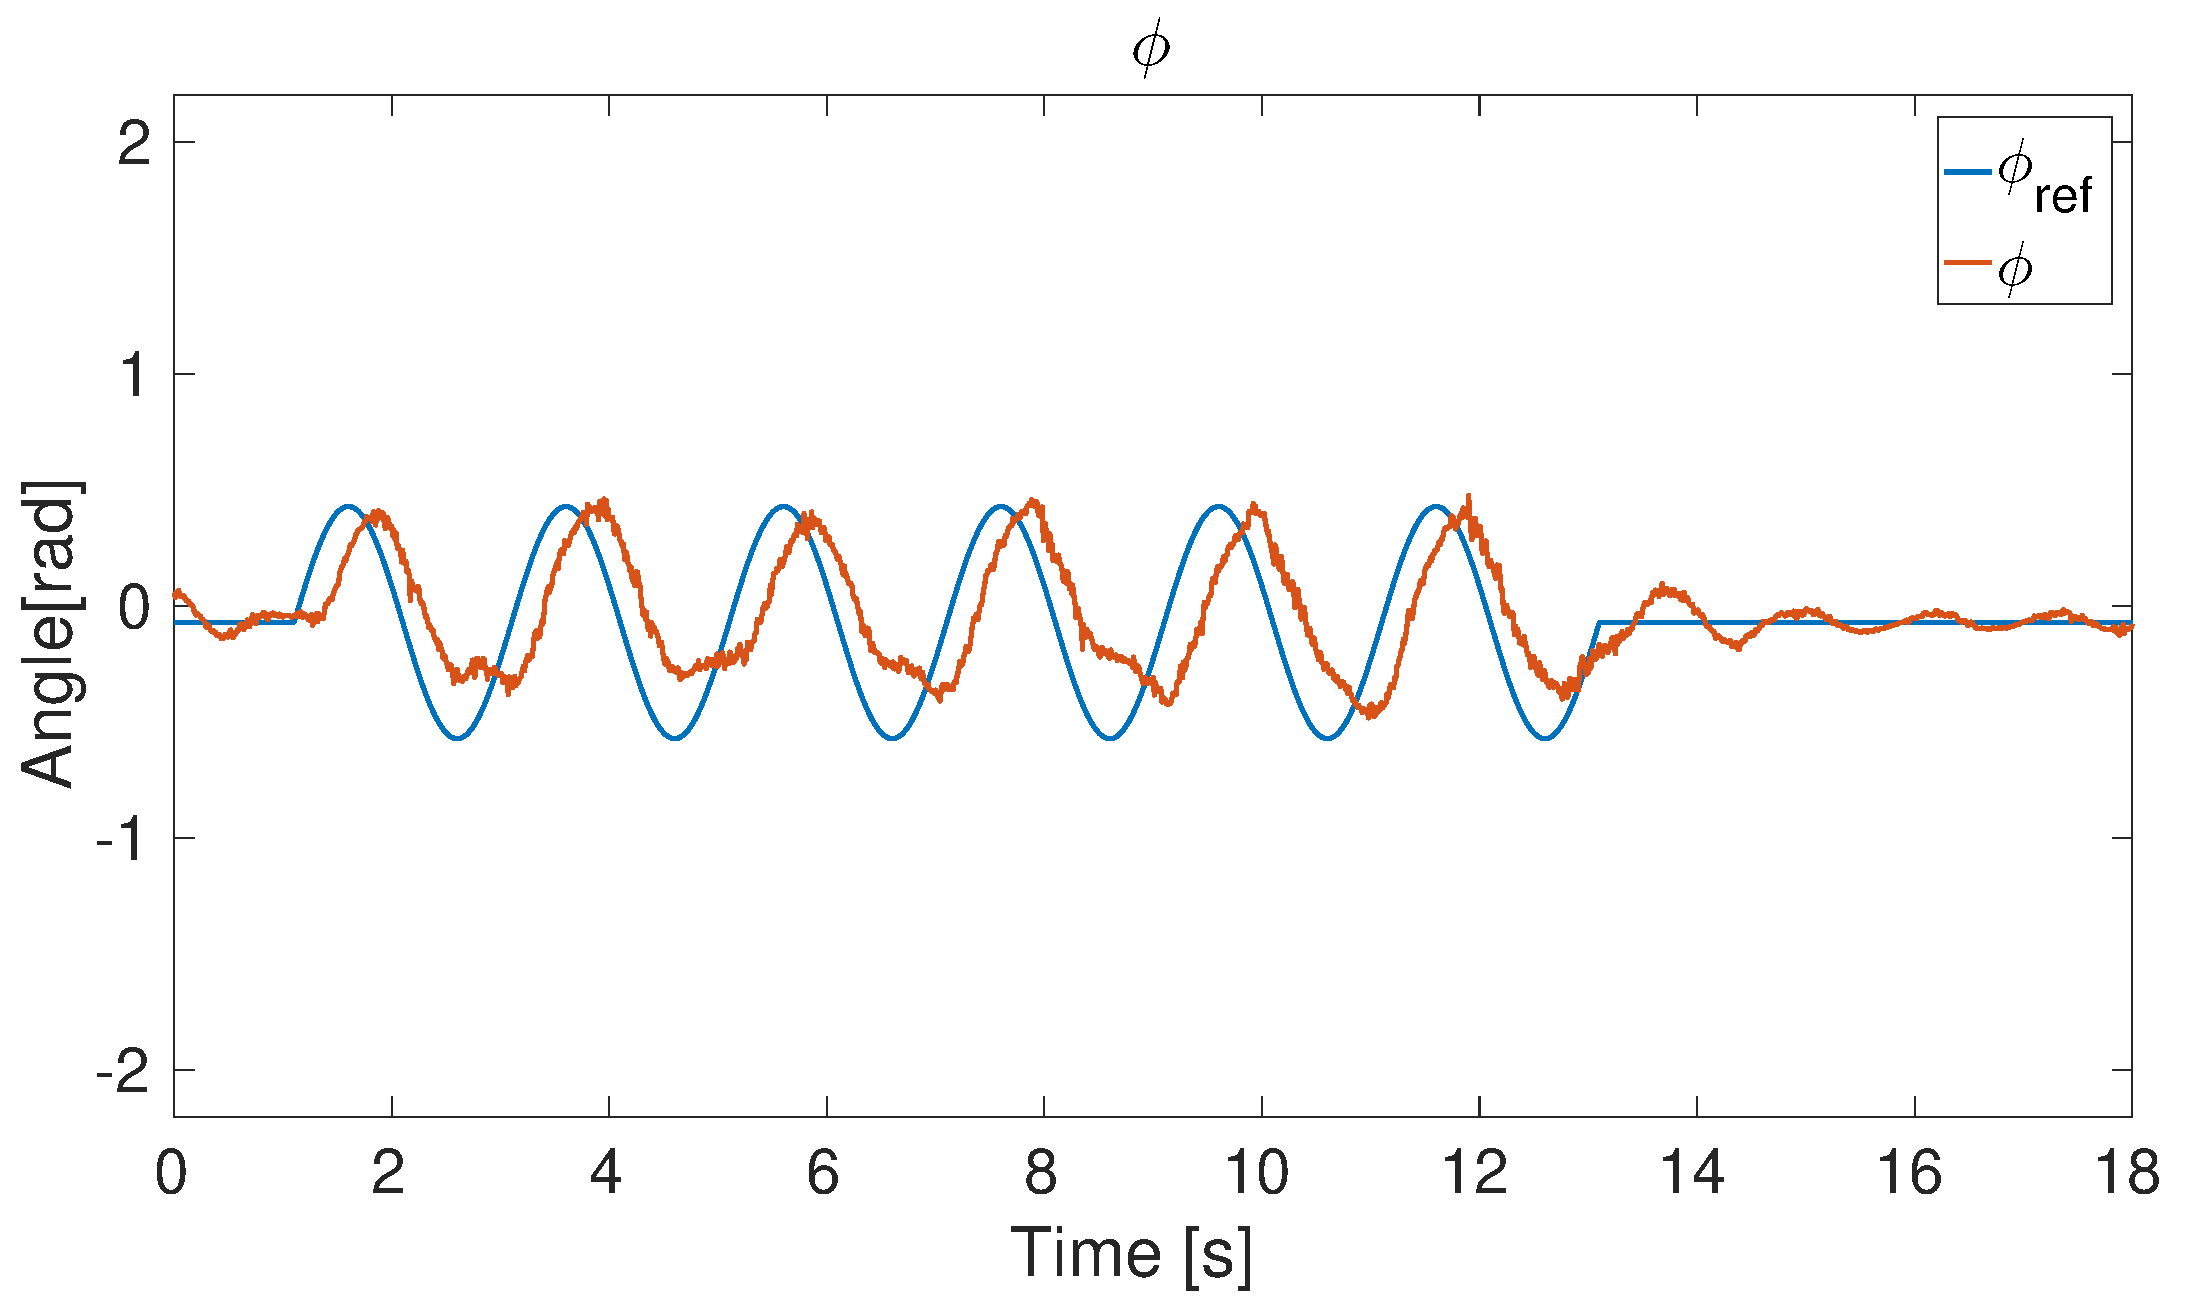
\includegraphics[width=0.4\textwidth]{testSinAllPhiA05}}
  \qquad
  \subfloat[][\label{fig:AppsimSinAll05RollAttitude} A sine signal with amplitude $0.5$ and frequency $0.5\hertz$ applied to the simulated \abbrROV in $\rollAngle$.]{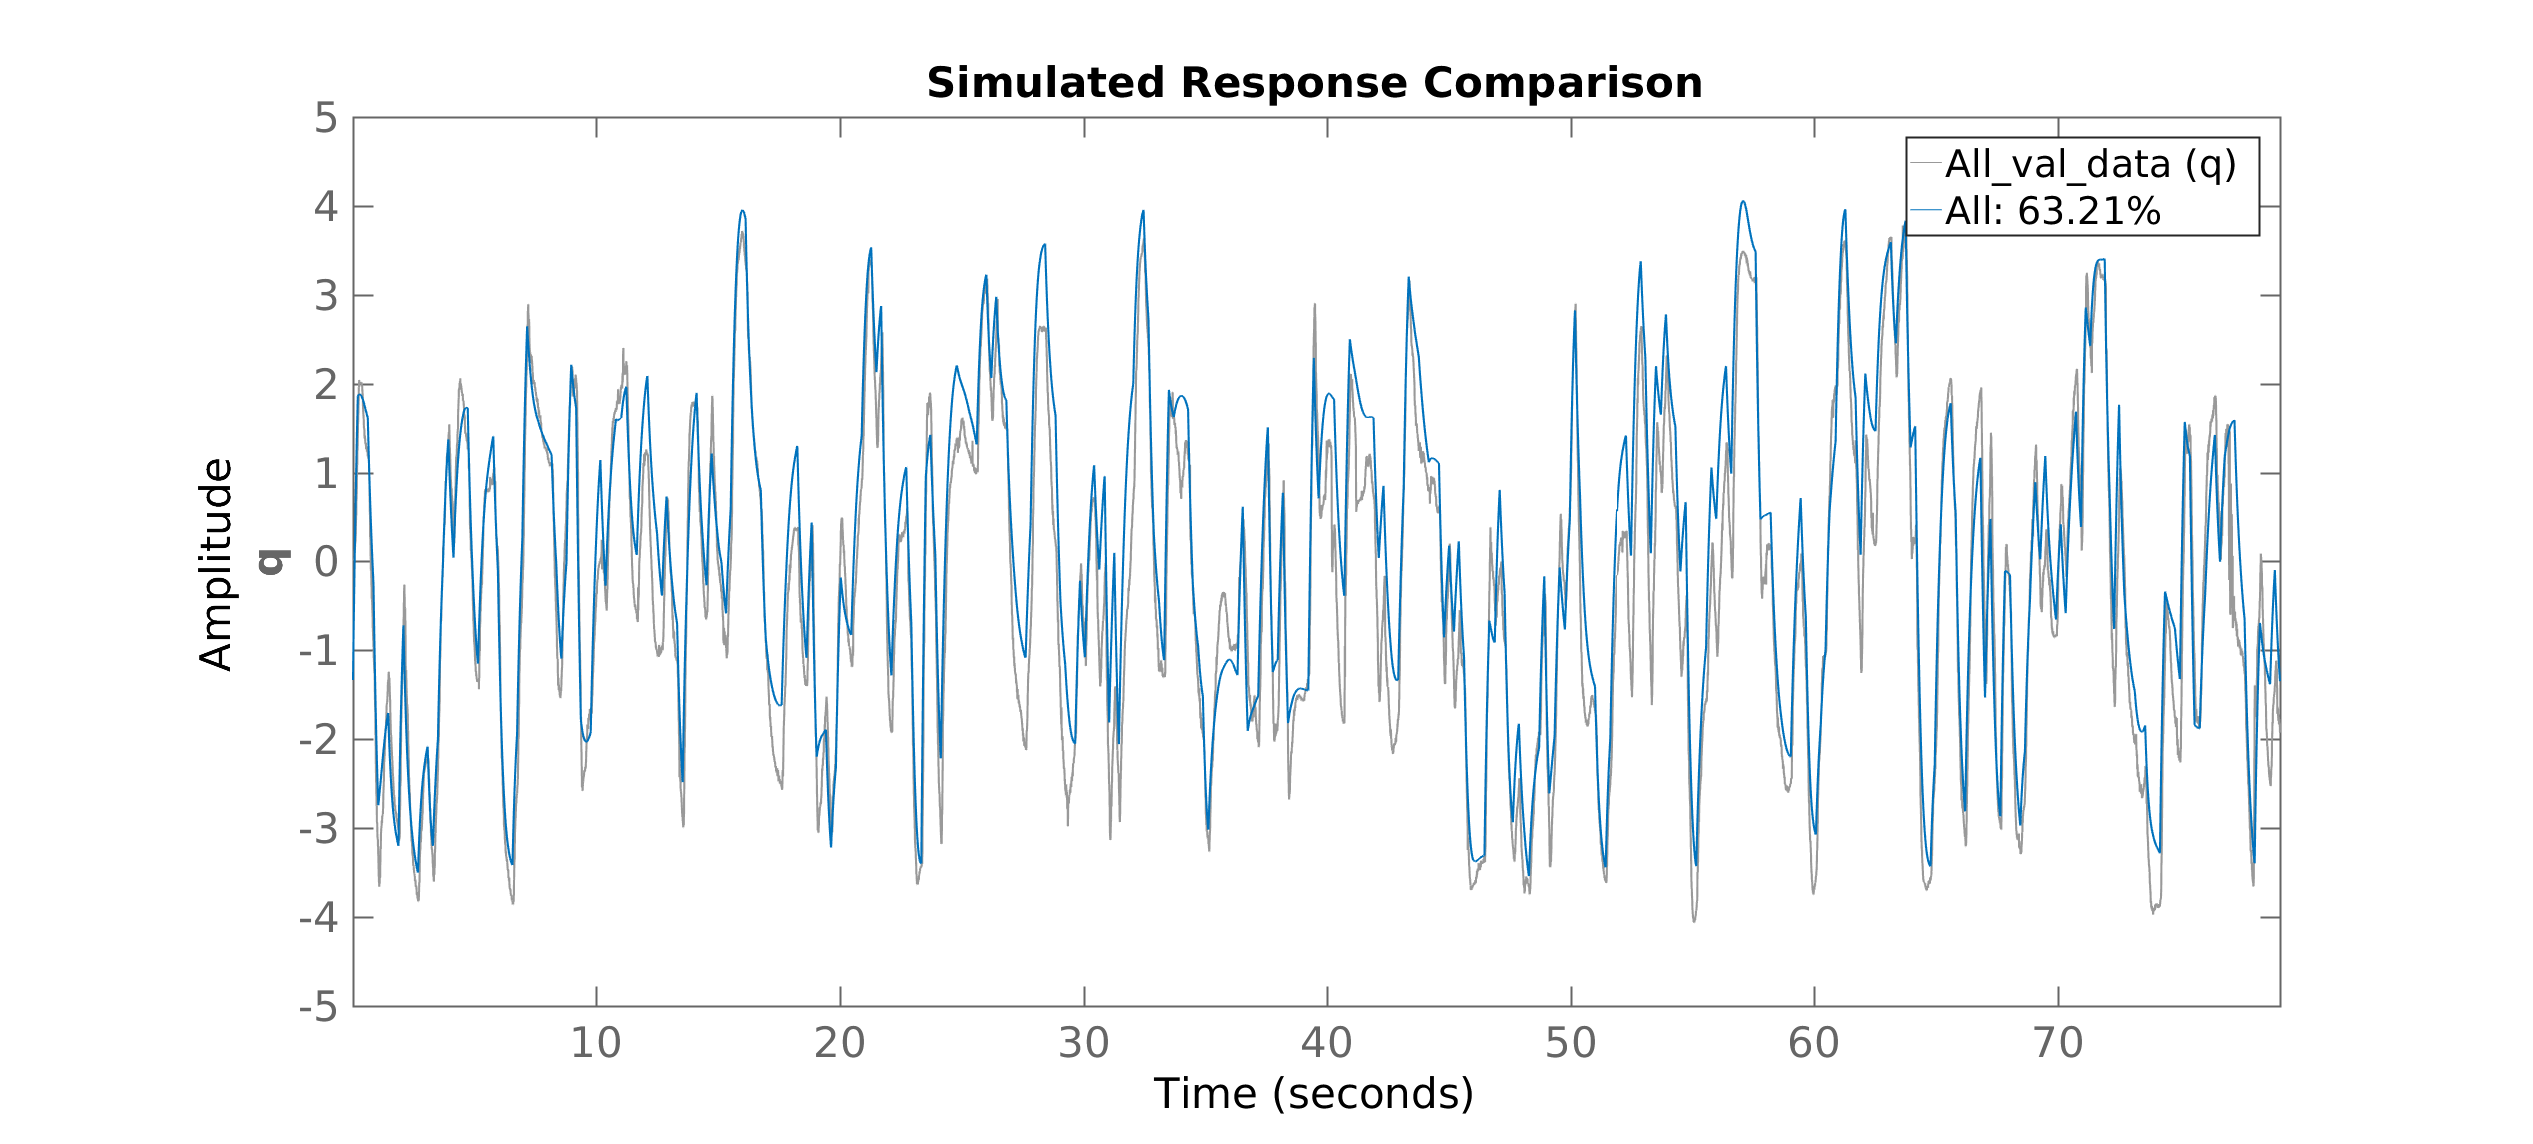
\includegraphics[width=0.4\textwidth]{velocityCompareq}}
  \qquad
  \subfloat[][\label{fig:AppTestSinAll05PitchAttitude} A sine signal with amplitude $0.5$ and frequency $0.5\hertz$ applied in $\pitchAngle$.]{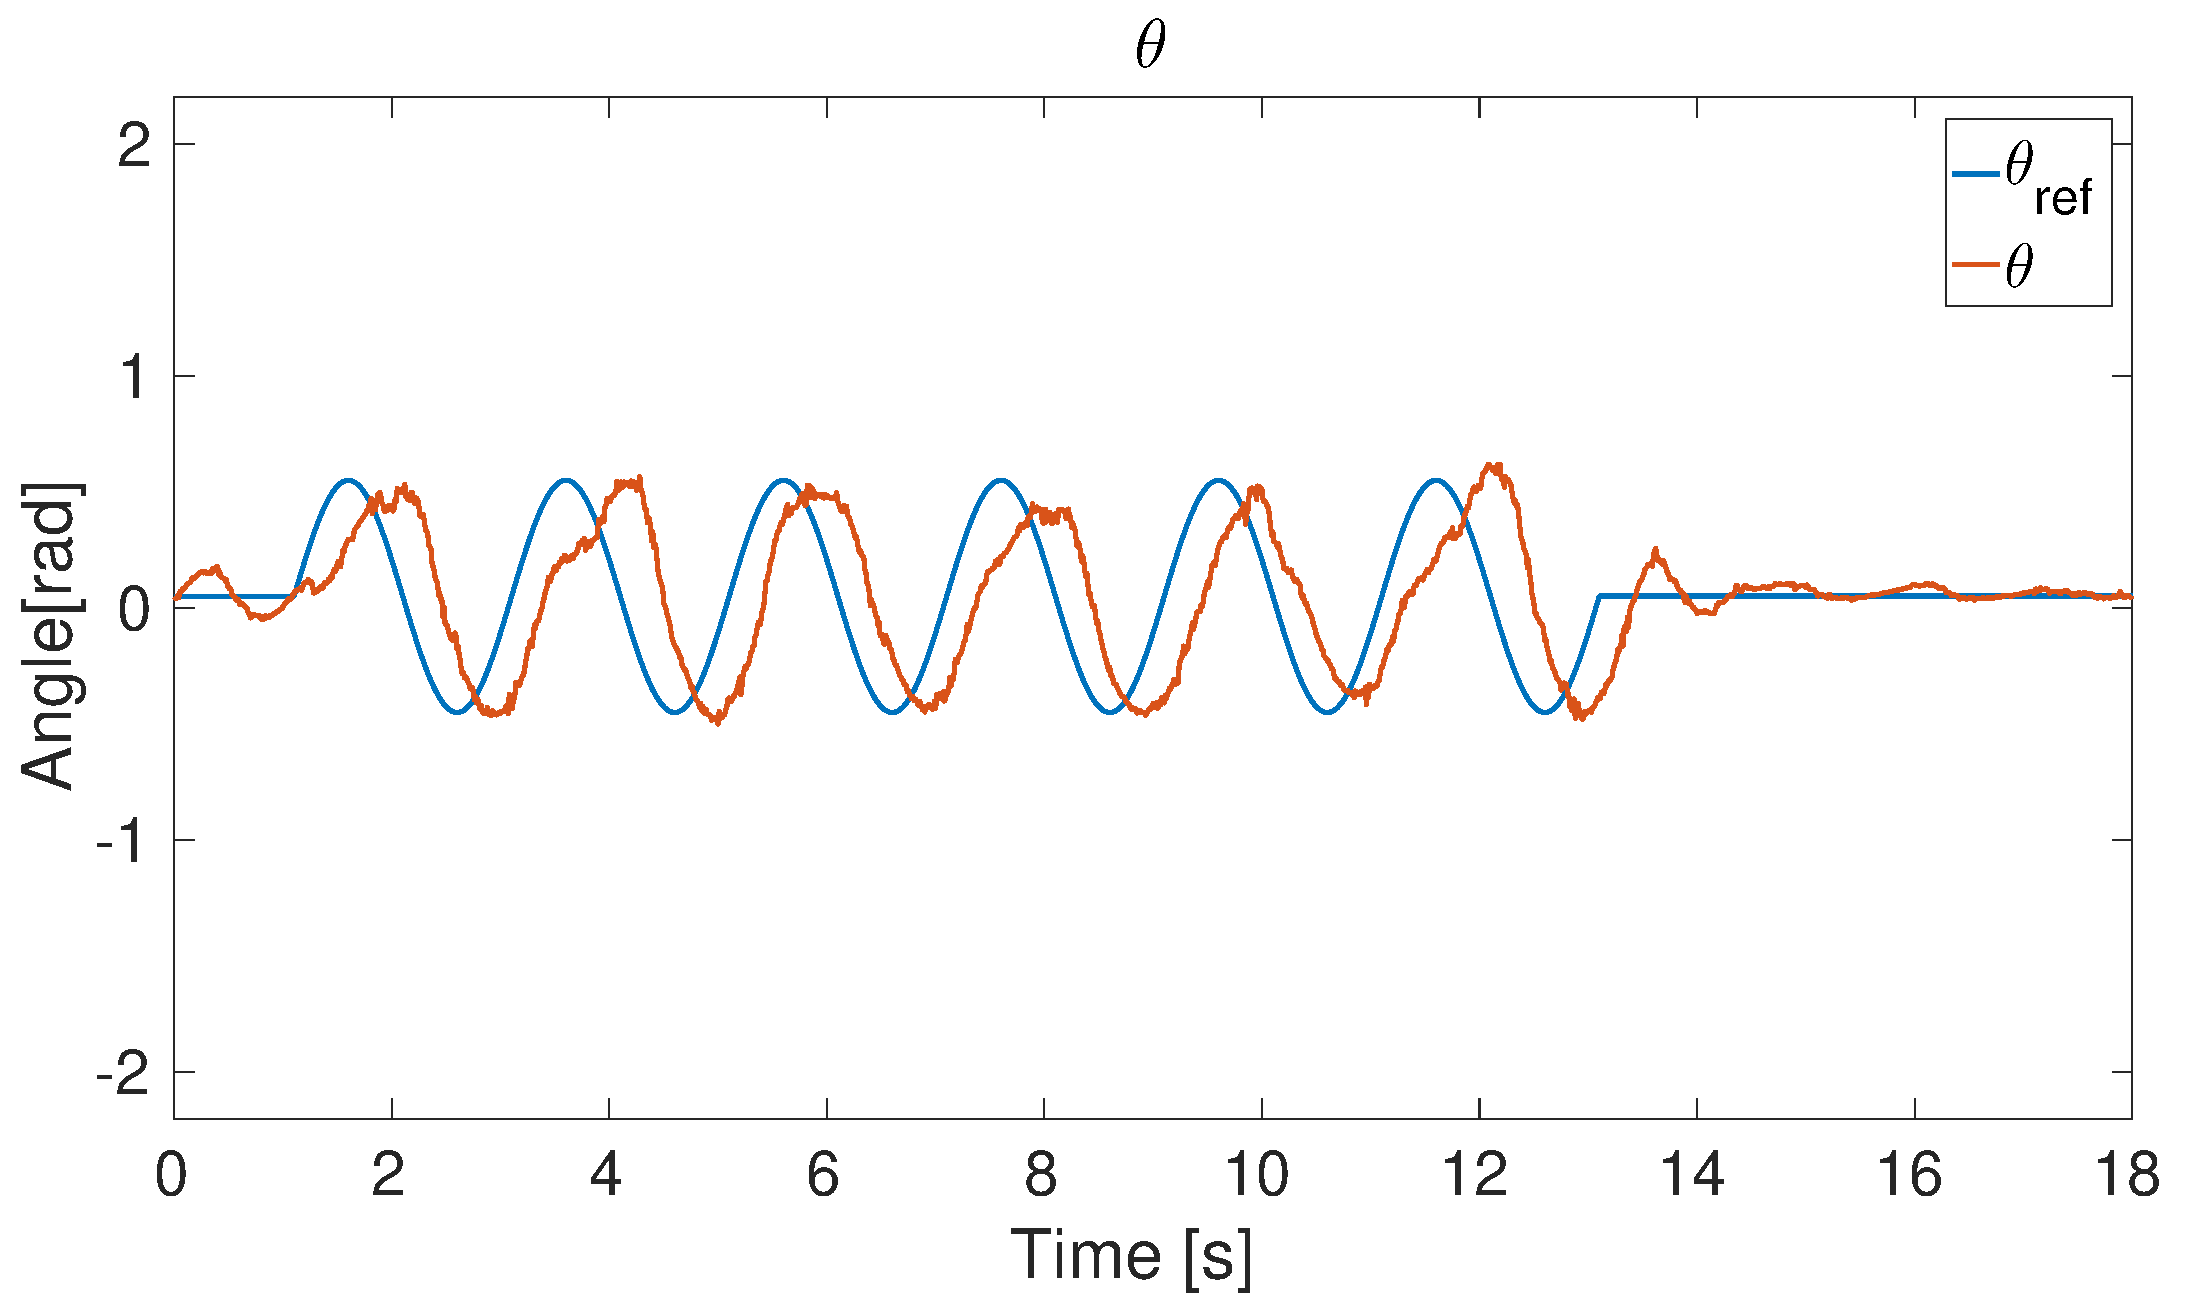
\includegraphics[width=0.4\textwidth]{testSinAllThetaA05}}
  \qquad
  \subfloat[][\label{fig:AppsimSinAll05PitchAttitude} A sine signal with amplitude $0.5$ and frequency $0.5\hertz$ applied to the simulated \abbrROV in $\pitchAngle$.]{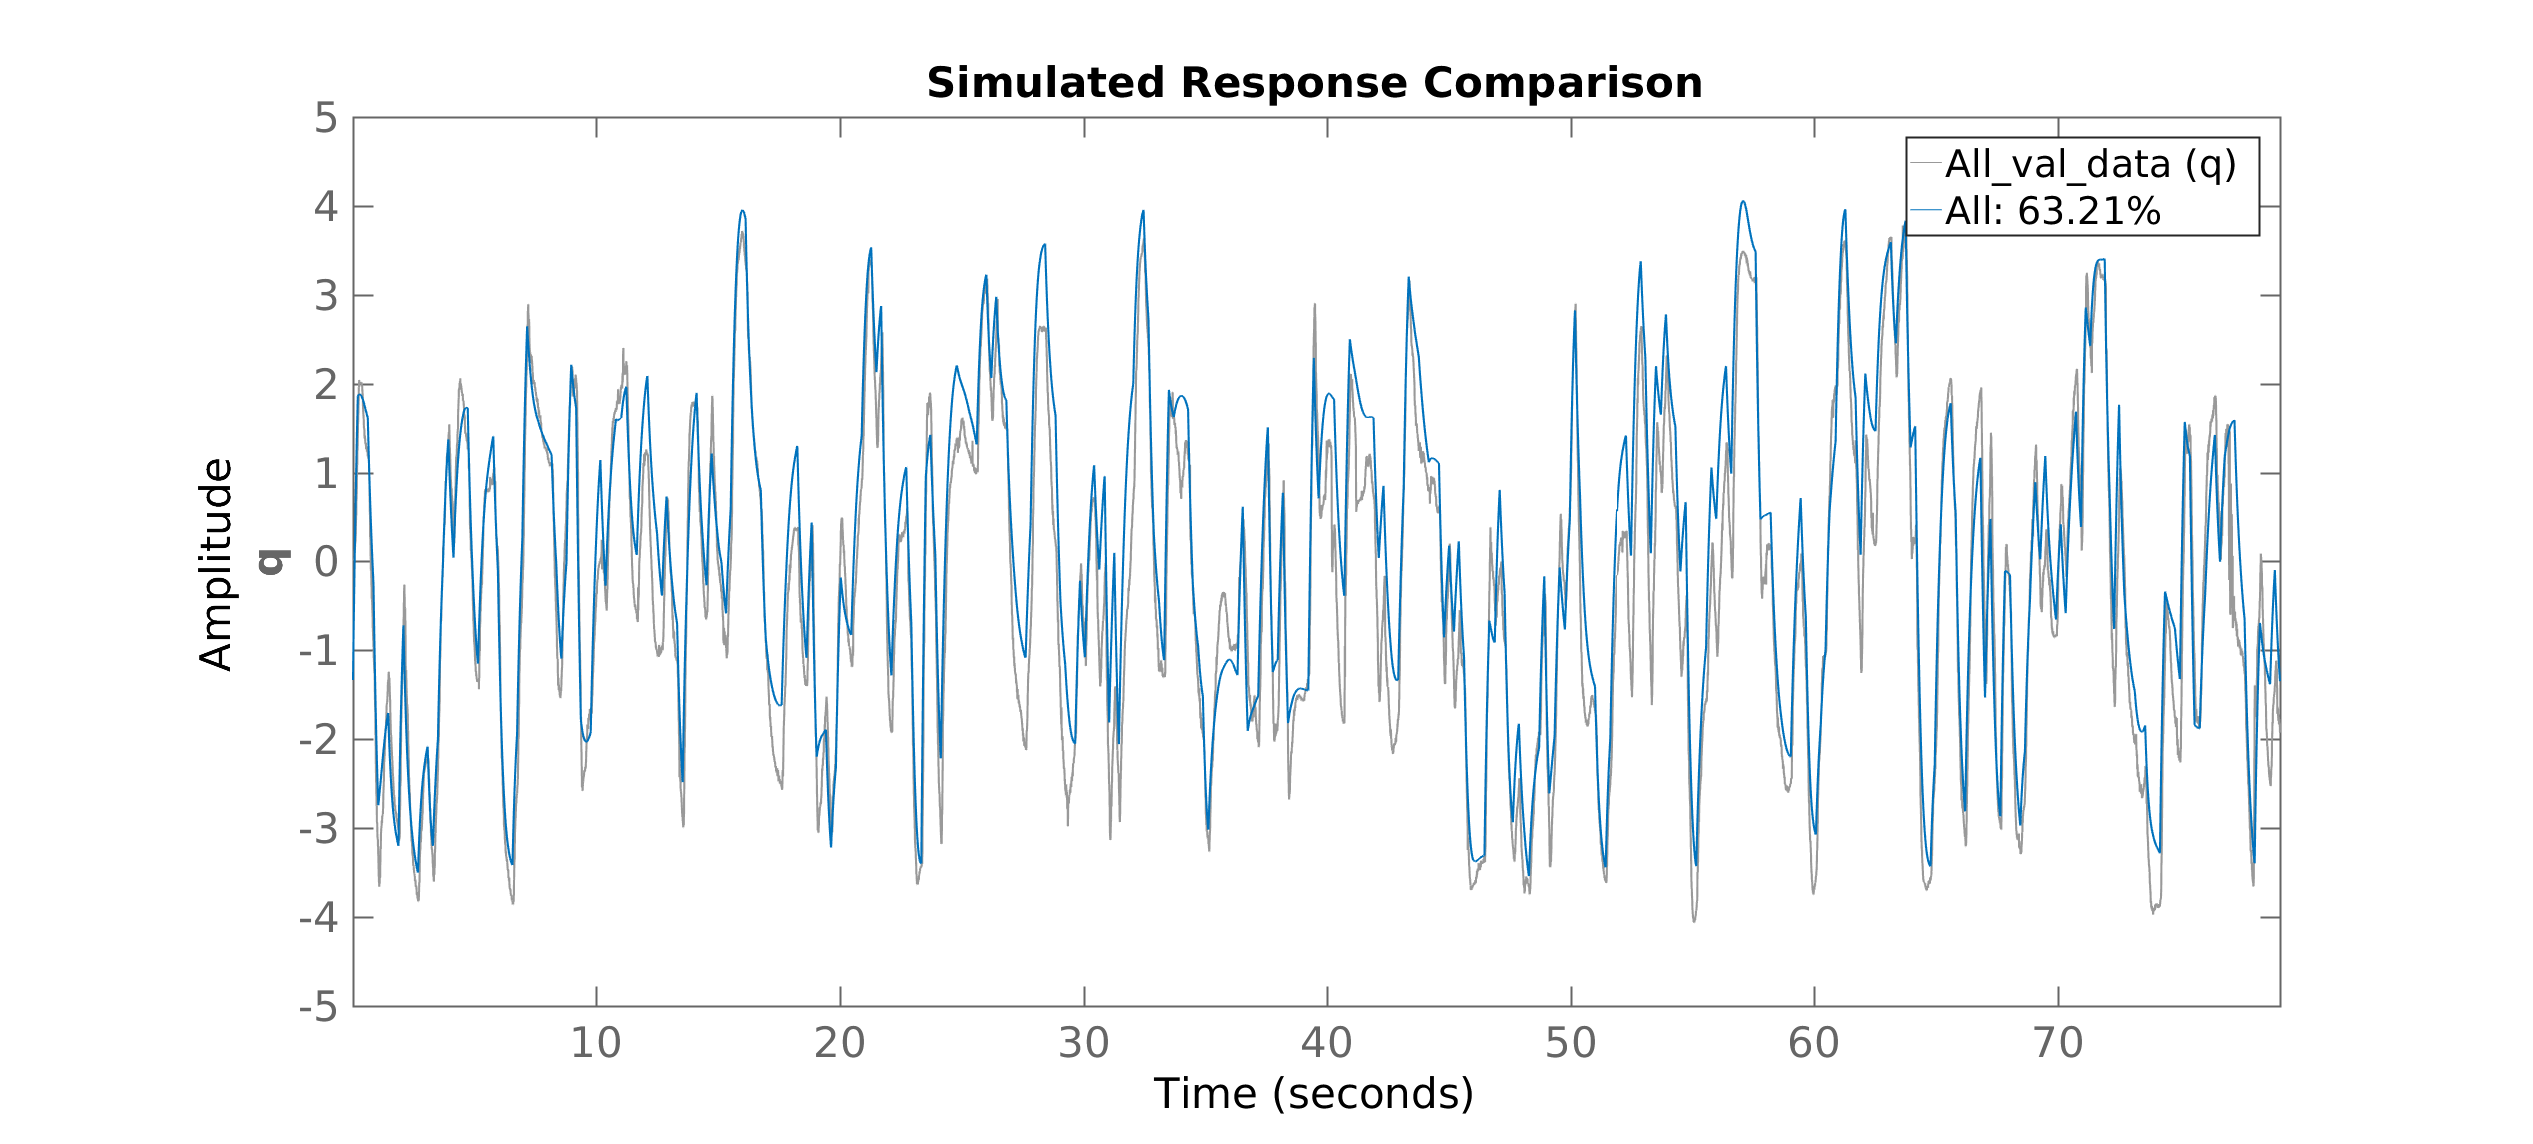
\includegraphics[width=0.4\textwidth]{velocityCompareq}}
  \qquad
  \subfloat[][\label{fig:AppTestSinAll05YawAttitude} A sine signal with amplitude $0.5$ and frequency $0.5\hertz$ applied in $\yawAngle$.]{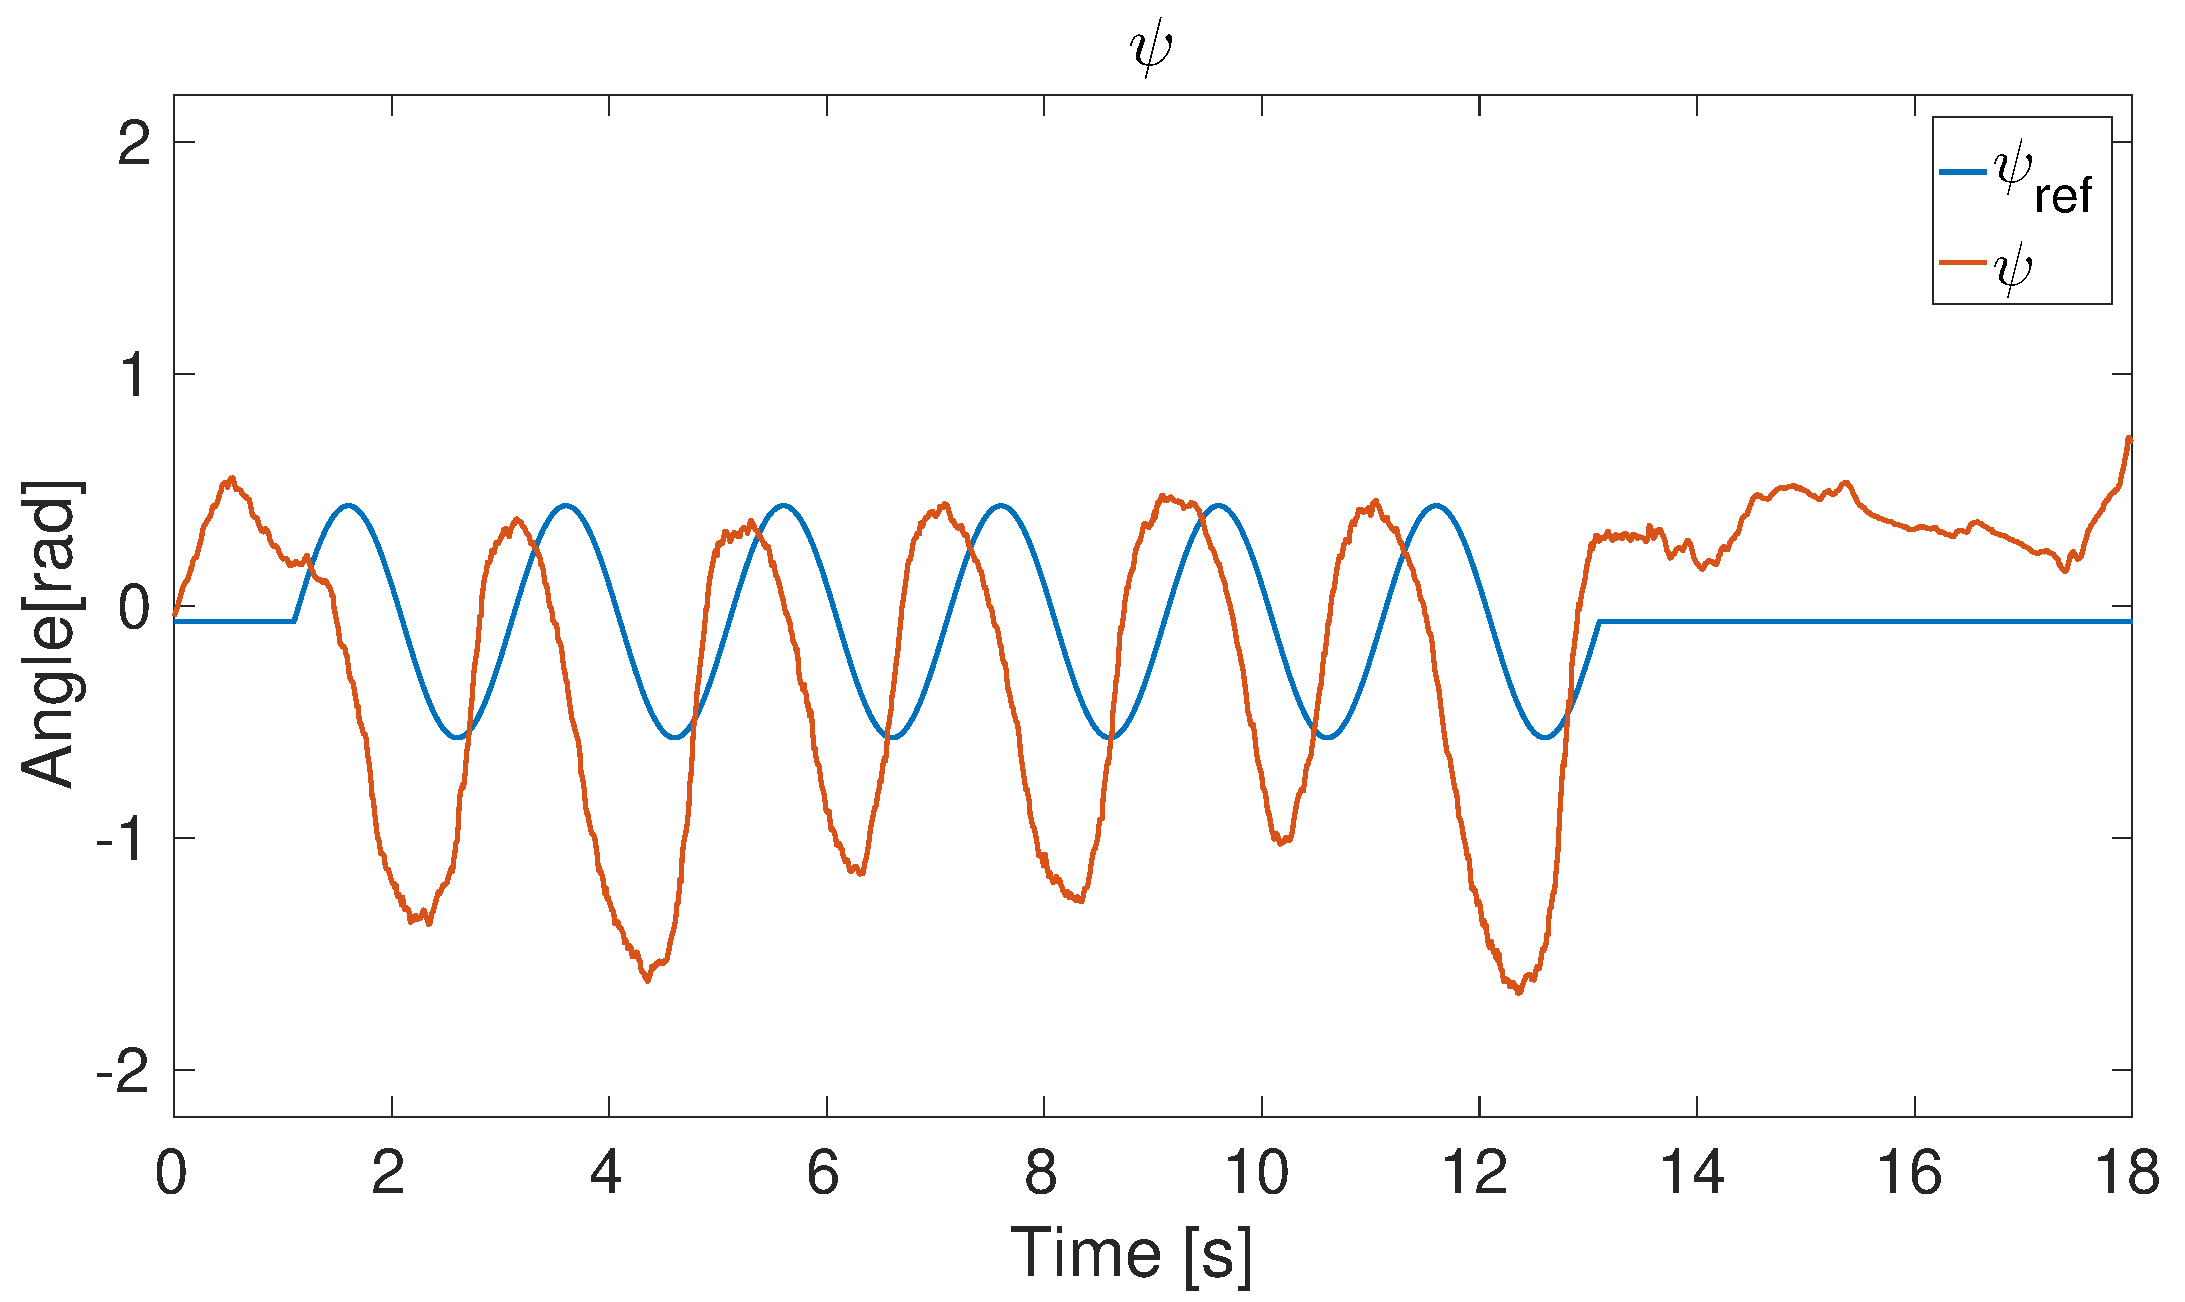
\includegraphics[width=0.4\textwidth]{testSinAllPsiA05}}
  \qquad
  \subfloat[][\label{fig:AppsimSinAll05YawAttitude} A sine signal with amplitude $0.5$ and frequency $0.5\hertz$ applied to the simulated \abbrROV in $\yawAngle$.]{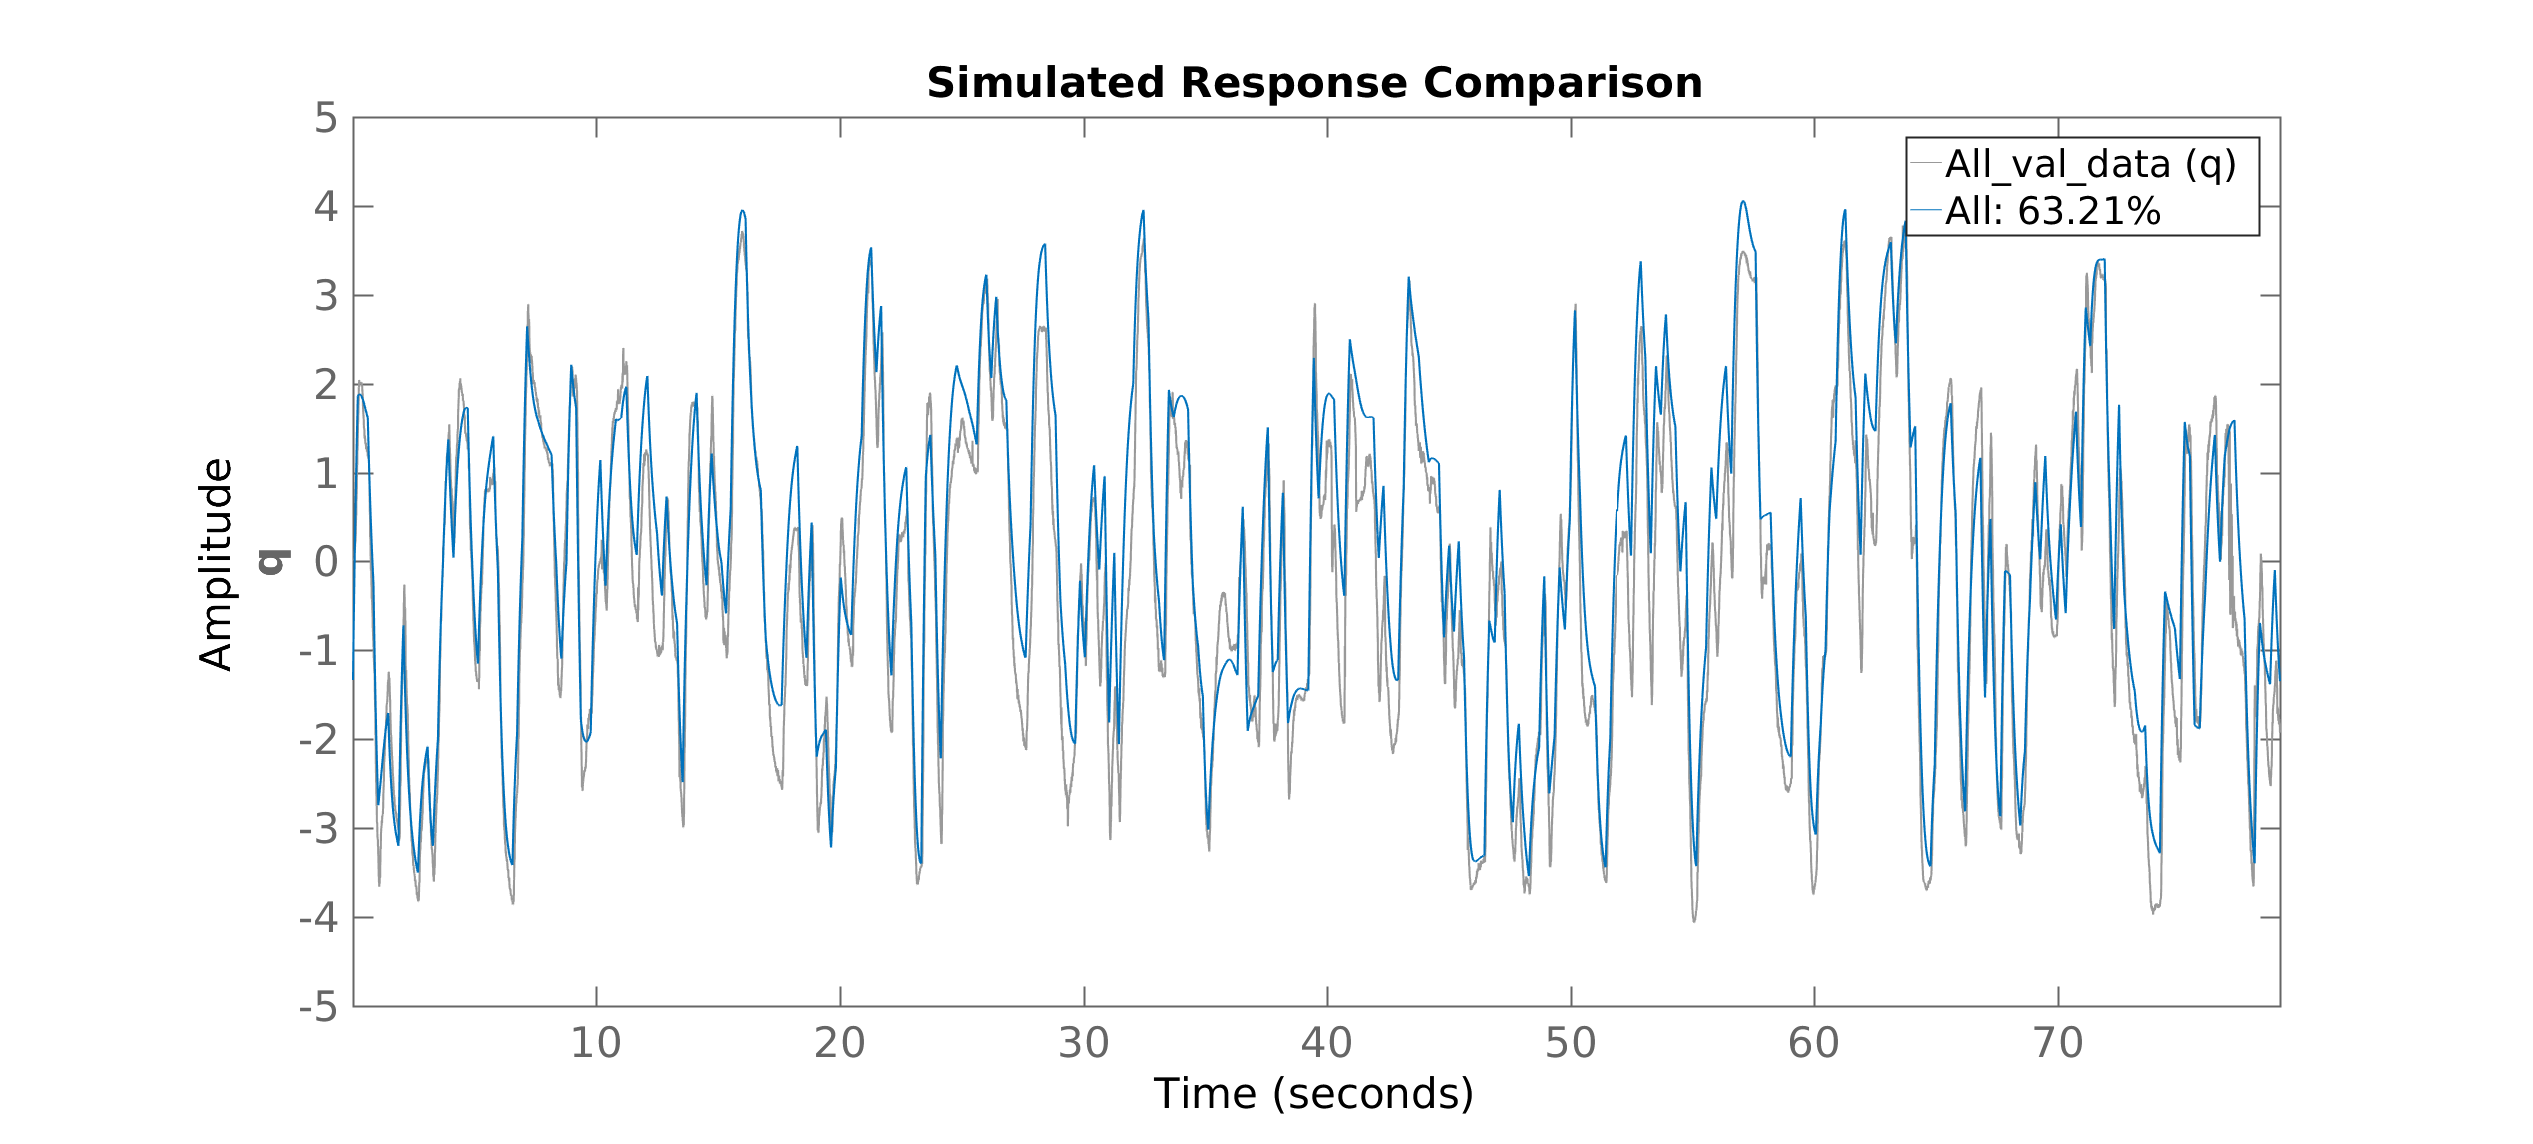
\includegraphics[width=0.4\textwidth]{velocityCompareq}}
  \caption{\label{fig:AppSinAll05Attitude}%
  Sine signals were applied in all attitude angles at the same time while using the attitude controller.}
\end{figure}

\begin{figure}
\centering
  \subfloat[][\label{fig:ApptestStepPhiTheta05RollAttitude} A smooth step applied in $\rollAngle$.]{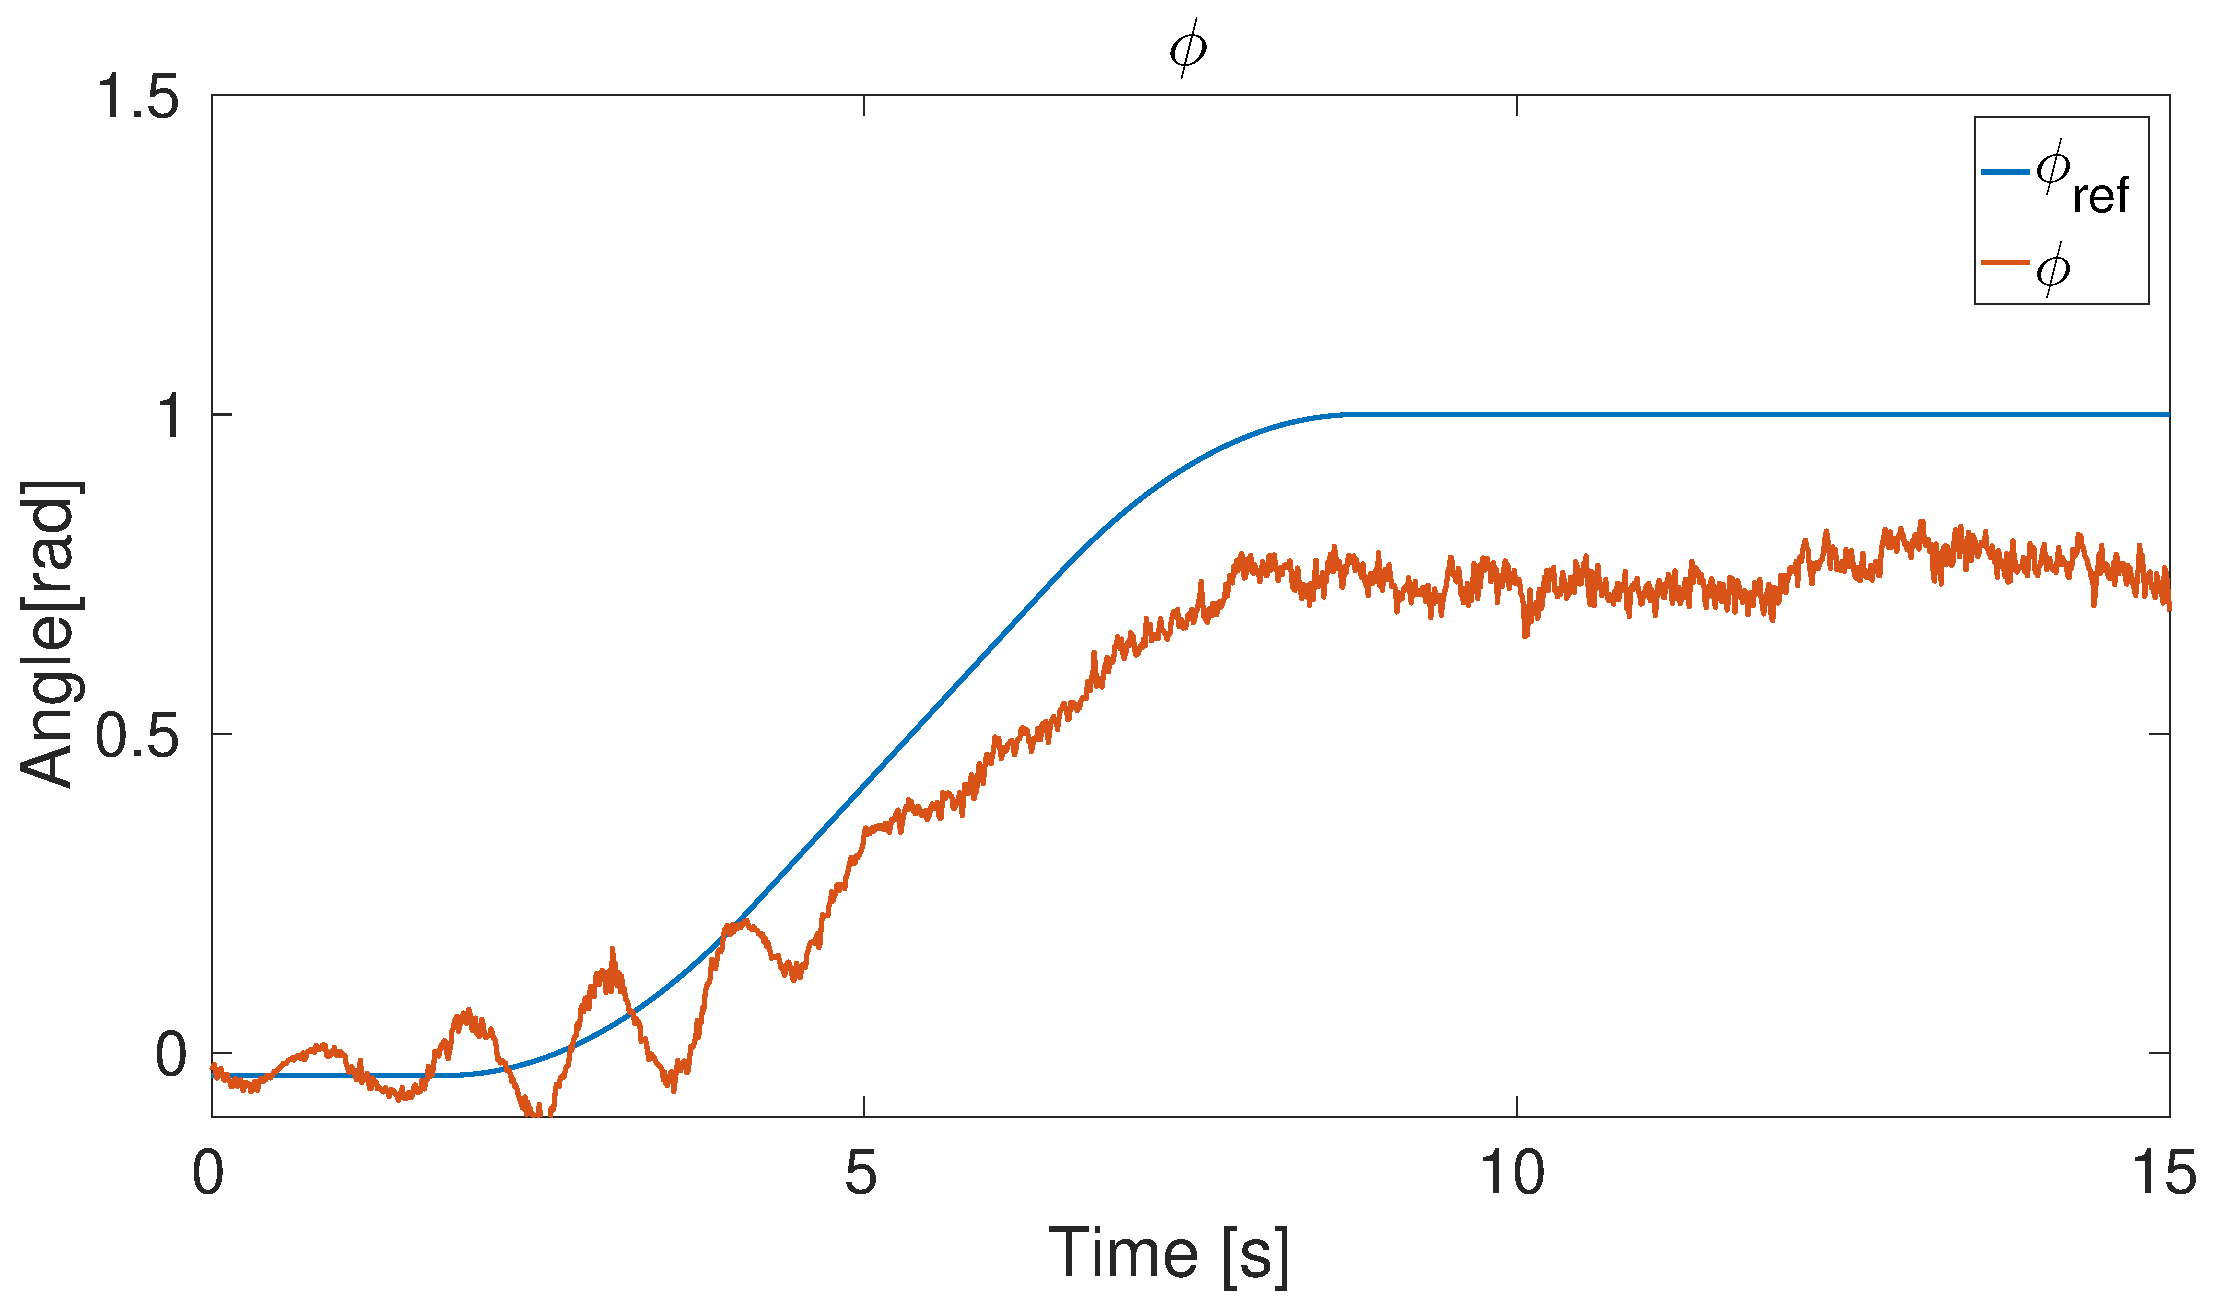
\includegraphics[width=0.4\textwidth]{testStepThetaPhiPhis3e10a1}}
  \qquad
  \subfloat[][\label{fig:AppsimStepPhiTheta05RollAttitude} A smooth step applied to the simulated \abbrROV in $\rollAngle$.]{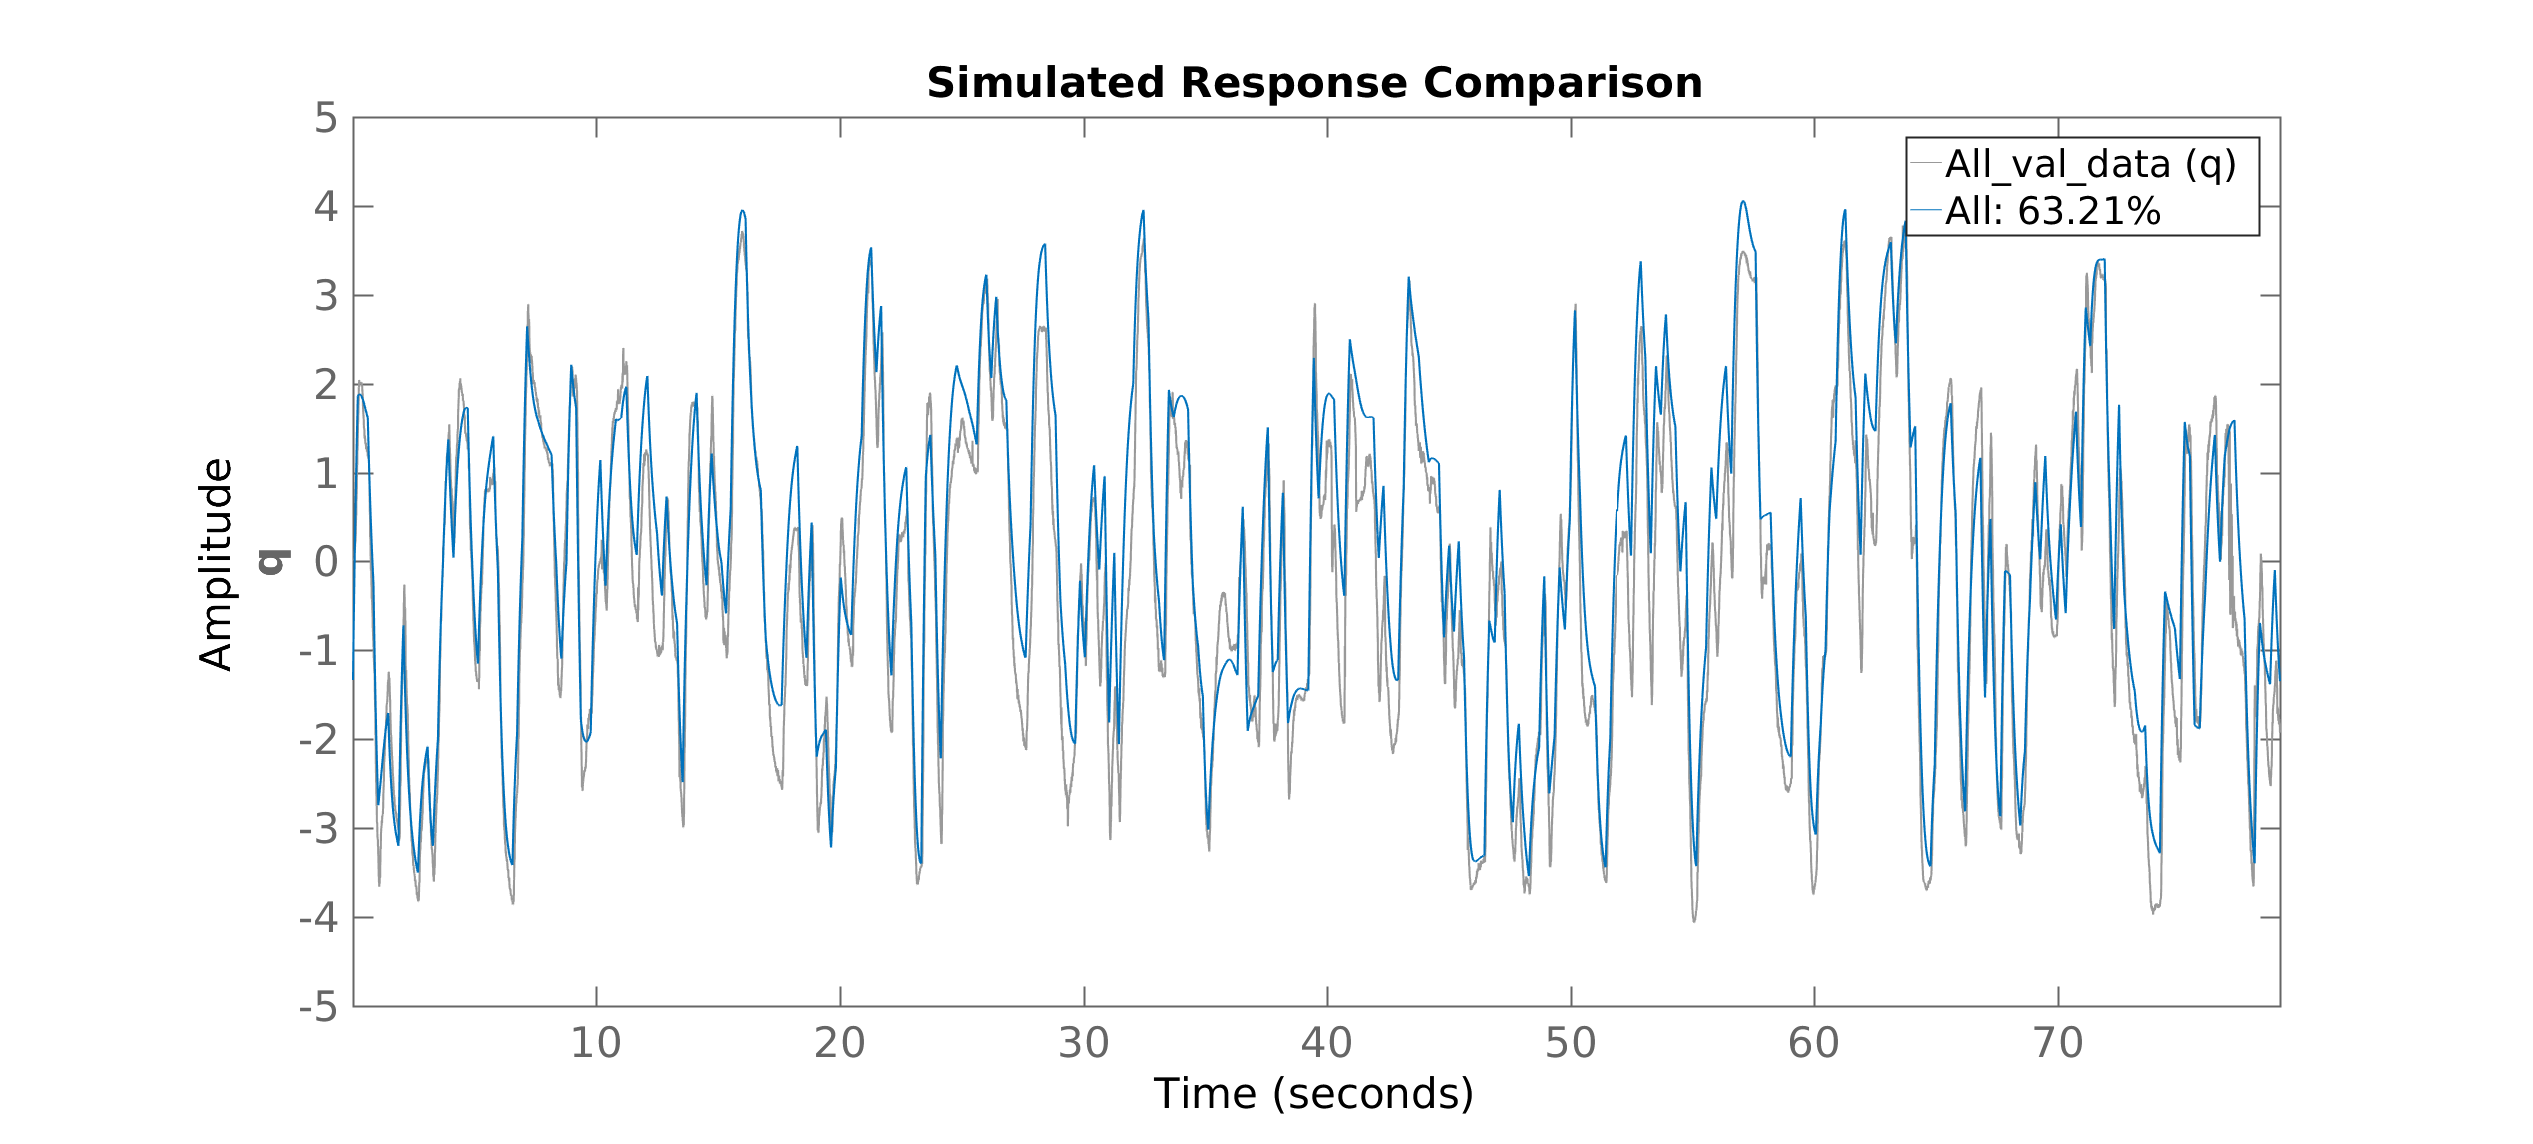
\includegraphics[width=0.4\textwidth]{velocityCompareq}}
  \qquad
  \subfloat[][\label{fig:ApptestStepPhiTheta05PitchAttitude} A smooth step applied in $\pitchAngle$.]{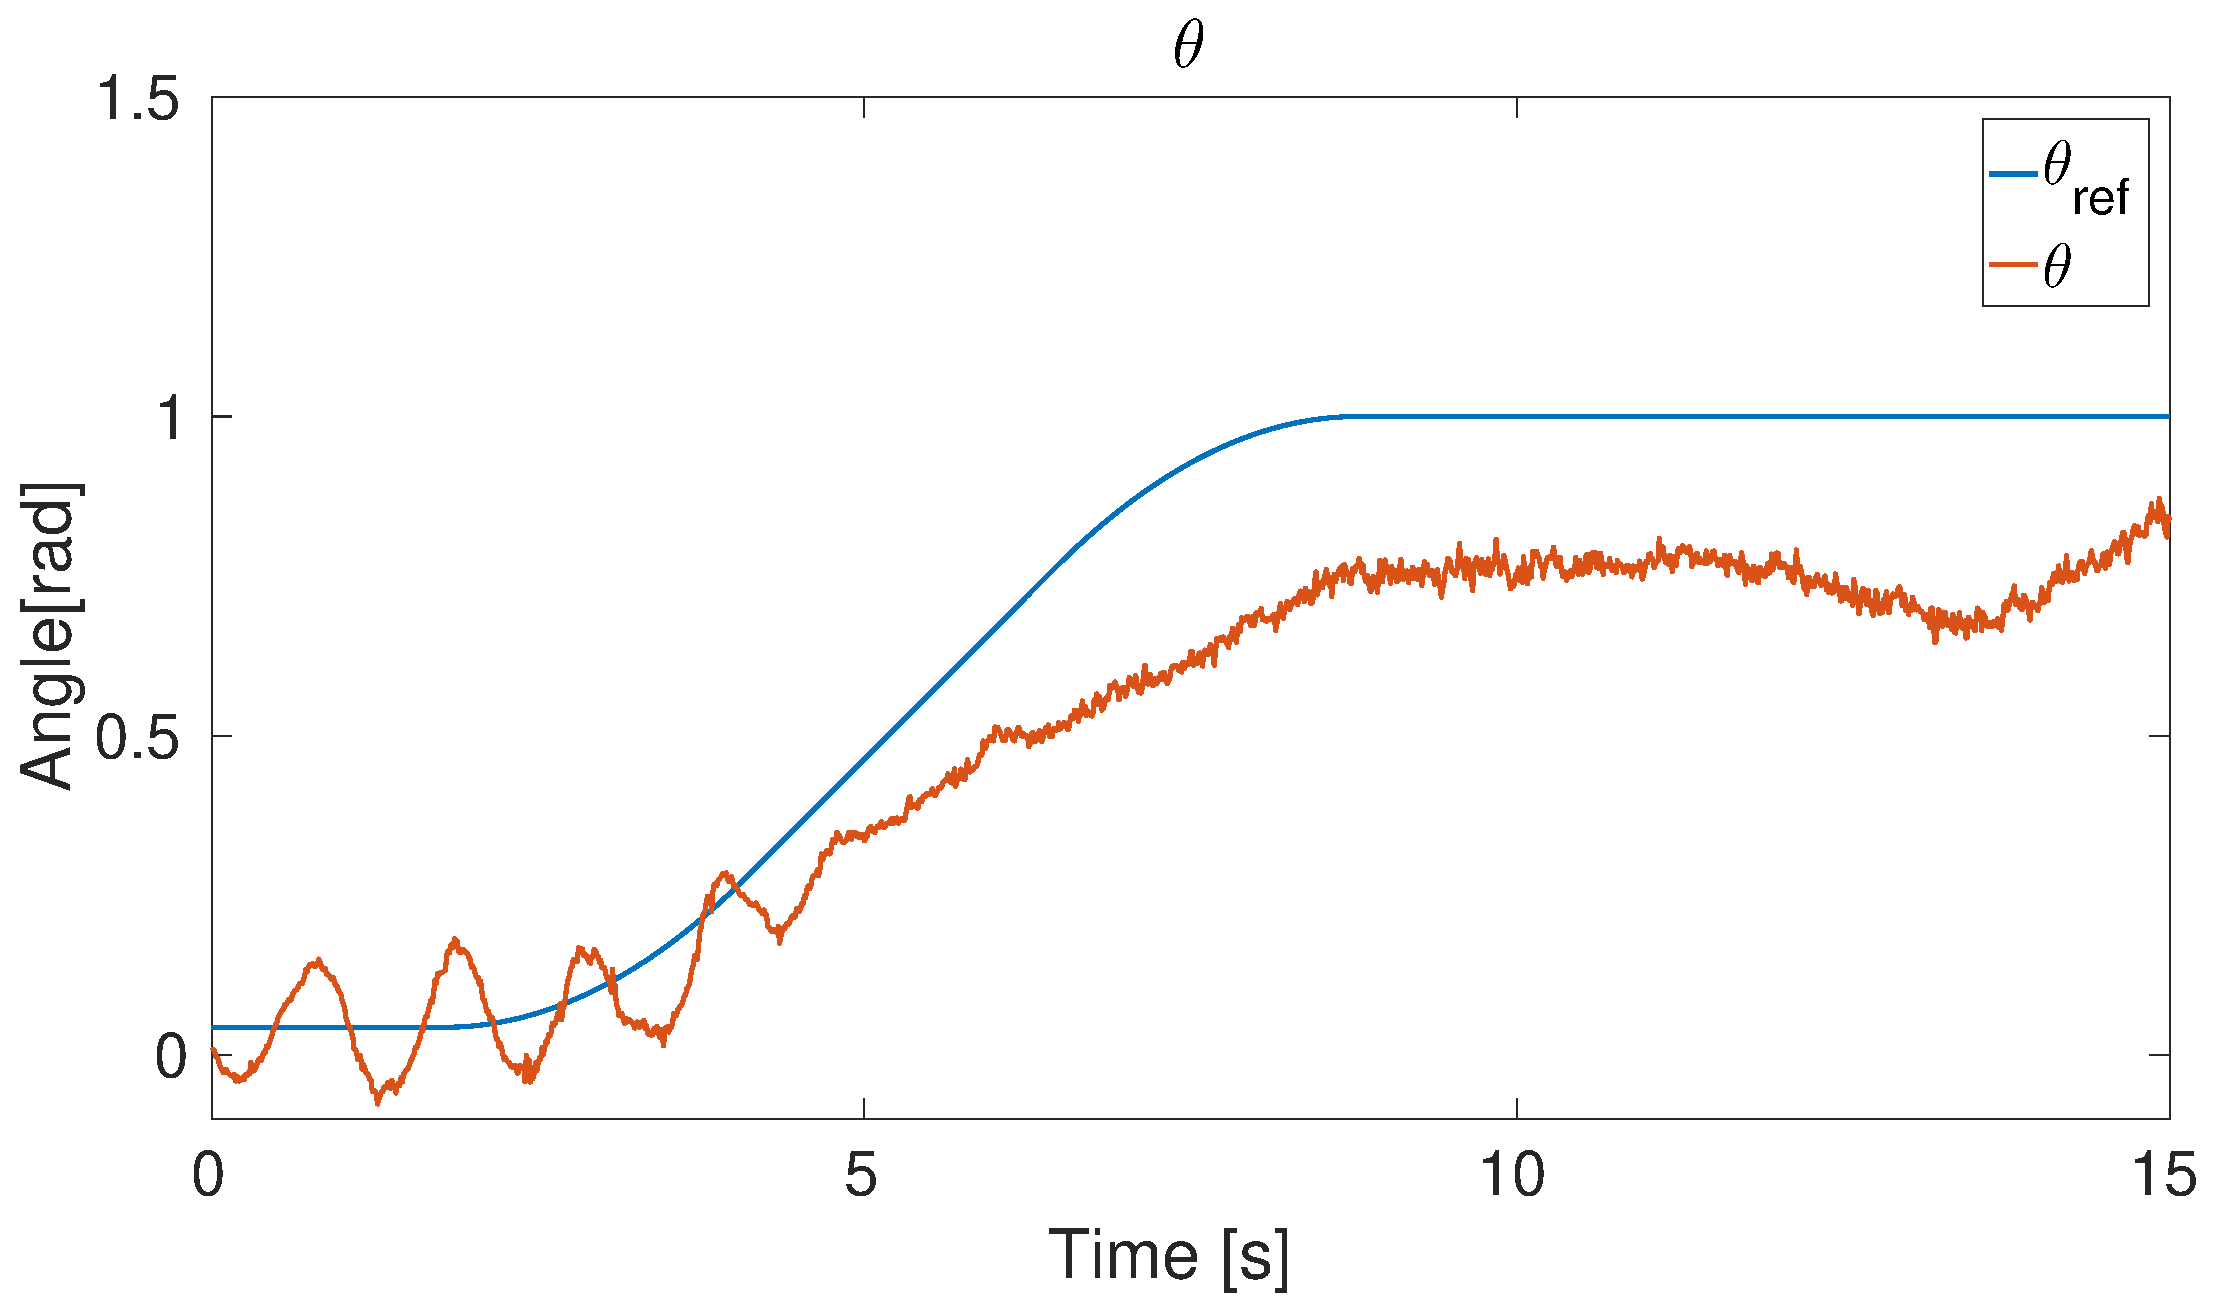
\includegraphics[width=0.4\textwidth]{testStepThetaPhiThetas3e10a1}}
  \qquad
  \subfloat[][\label{fig:AppsimStepPhiTheta05PitchAttitude} A smooth step applied to the simulated \abbrROV in $\pitchAngle$.]{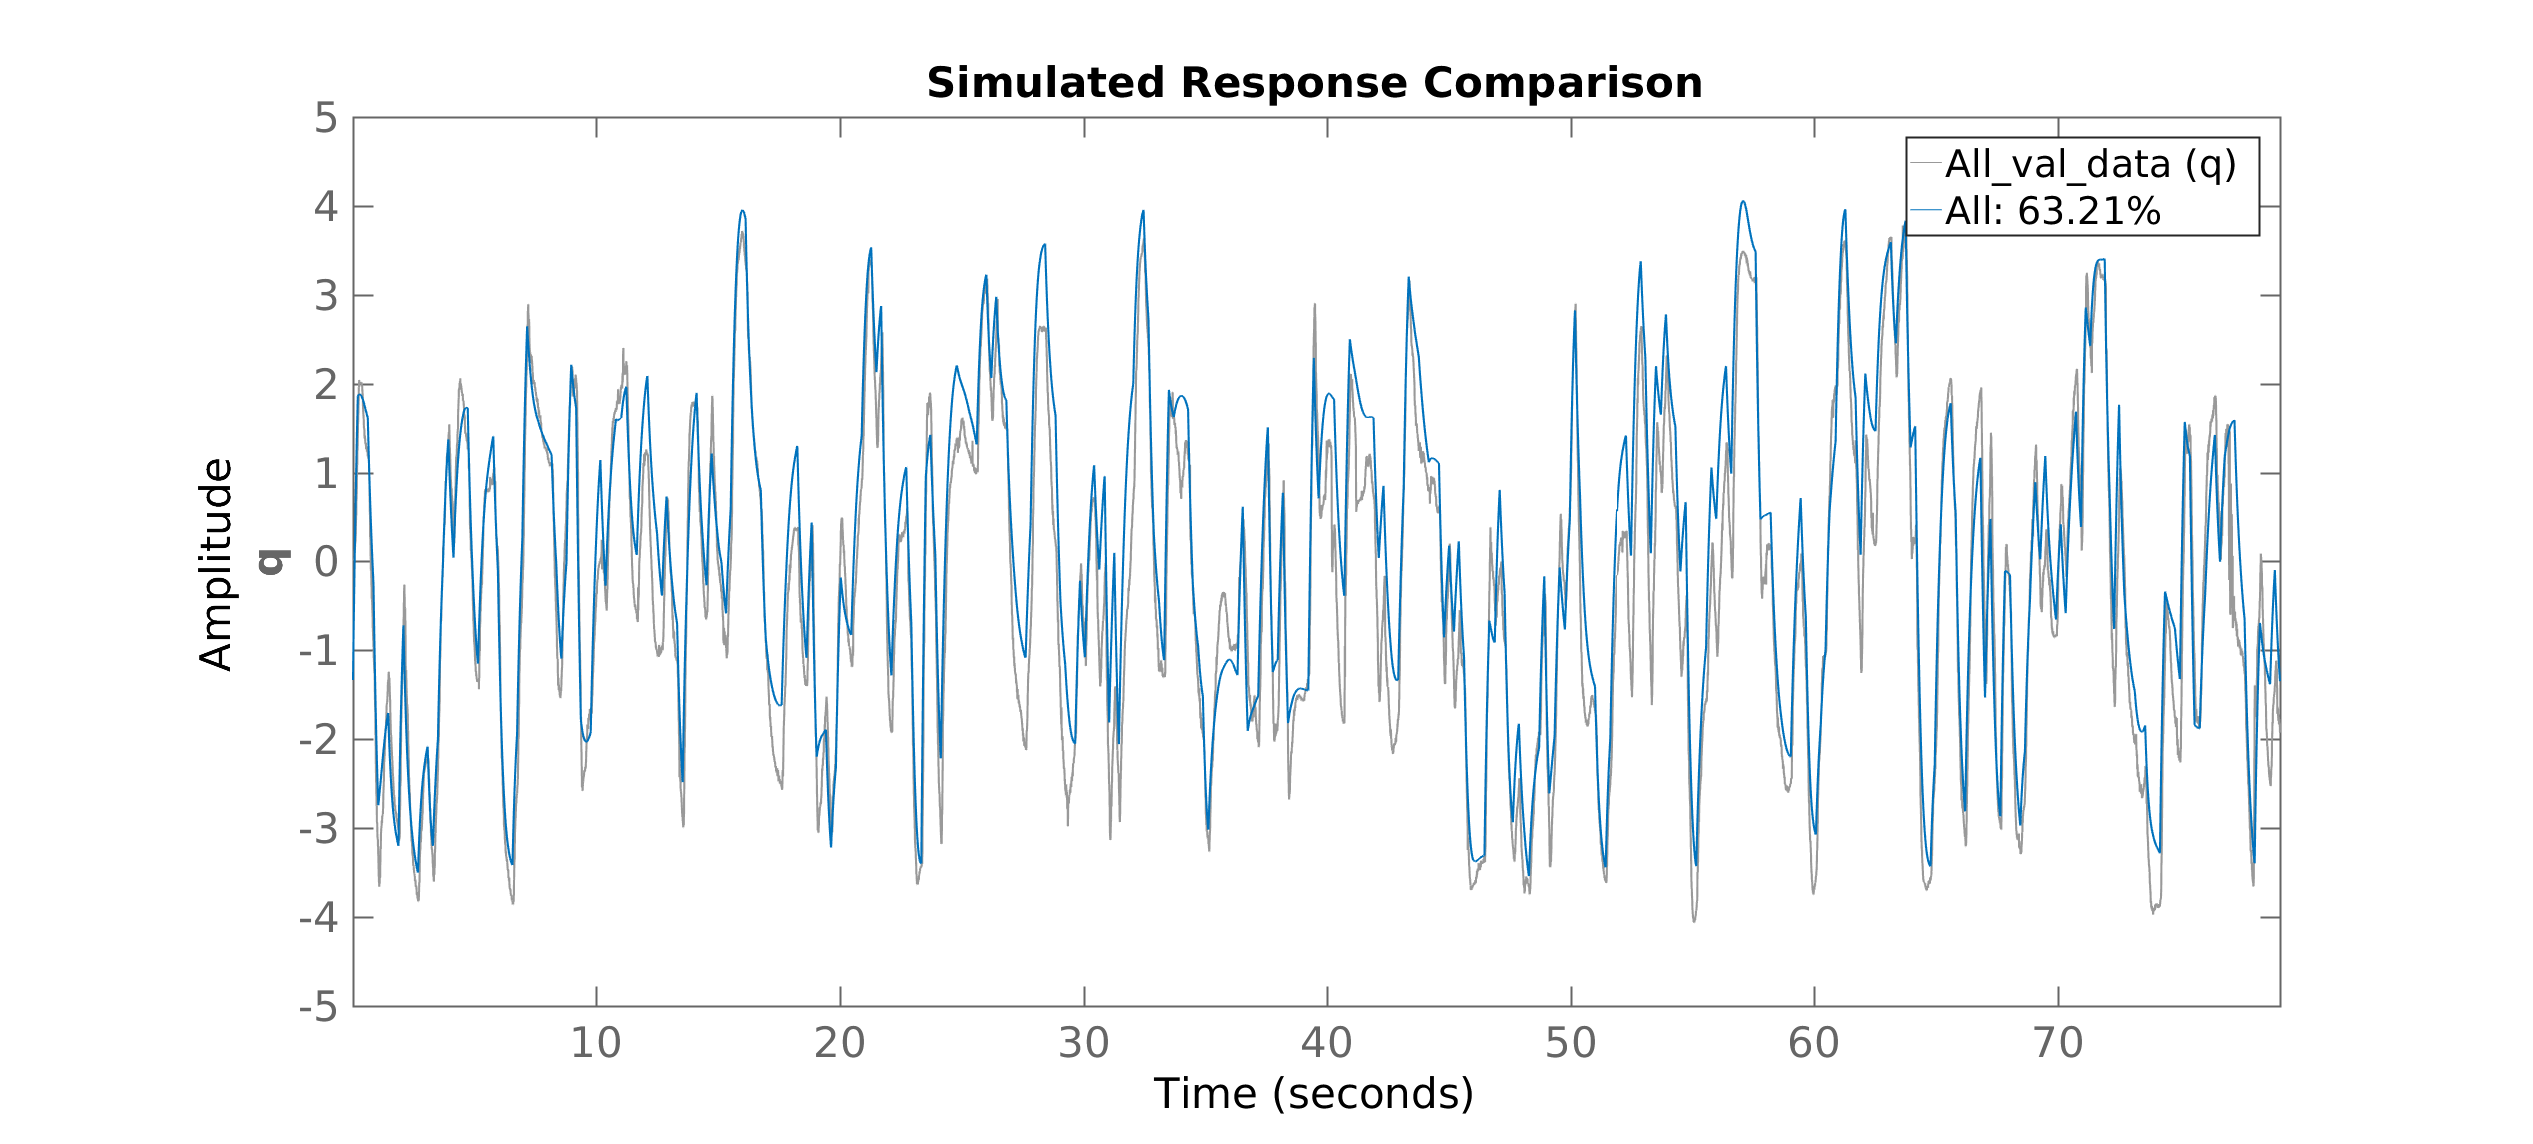
\includegraphics[width=0.4\textwidth]{velocityCompareq}}
  \caption{\label{fig:AppStepPhiThetaAttitude}%
  Smooth steps were applied in \pitchAngle and \rollAngle at the same time while using the attitude controller. The attitude angle \yawAngle was kept free during the test.}
\end{figure}

%%%%%%%%%%%%%%%%%%%%%%%%%%%Rate%%%%%%%%%%%%%%%%
\begin{figure}[tbp]
  \centering
  \subfloat[][\label{fig:ApptestStepP} A smooth step applied in $\rollVelocity$.]{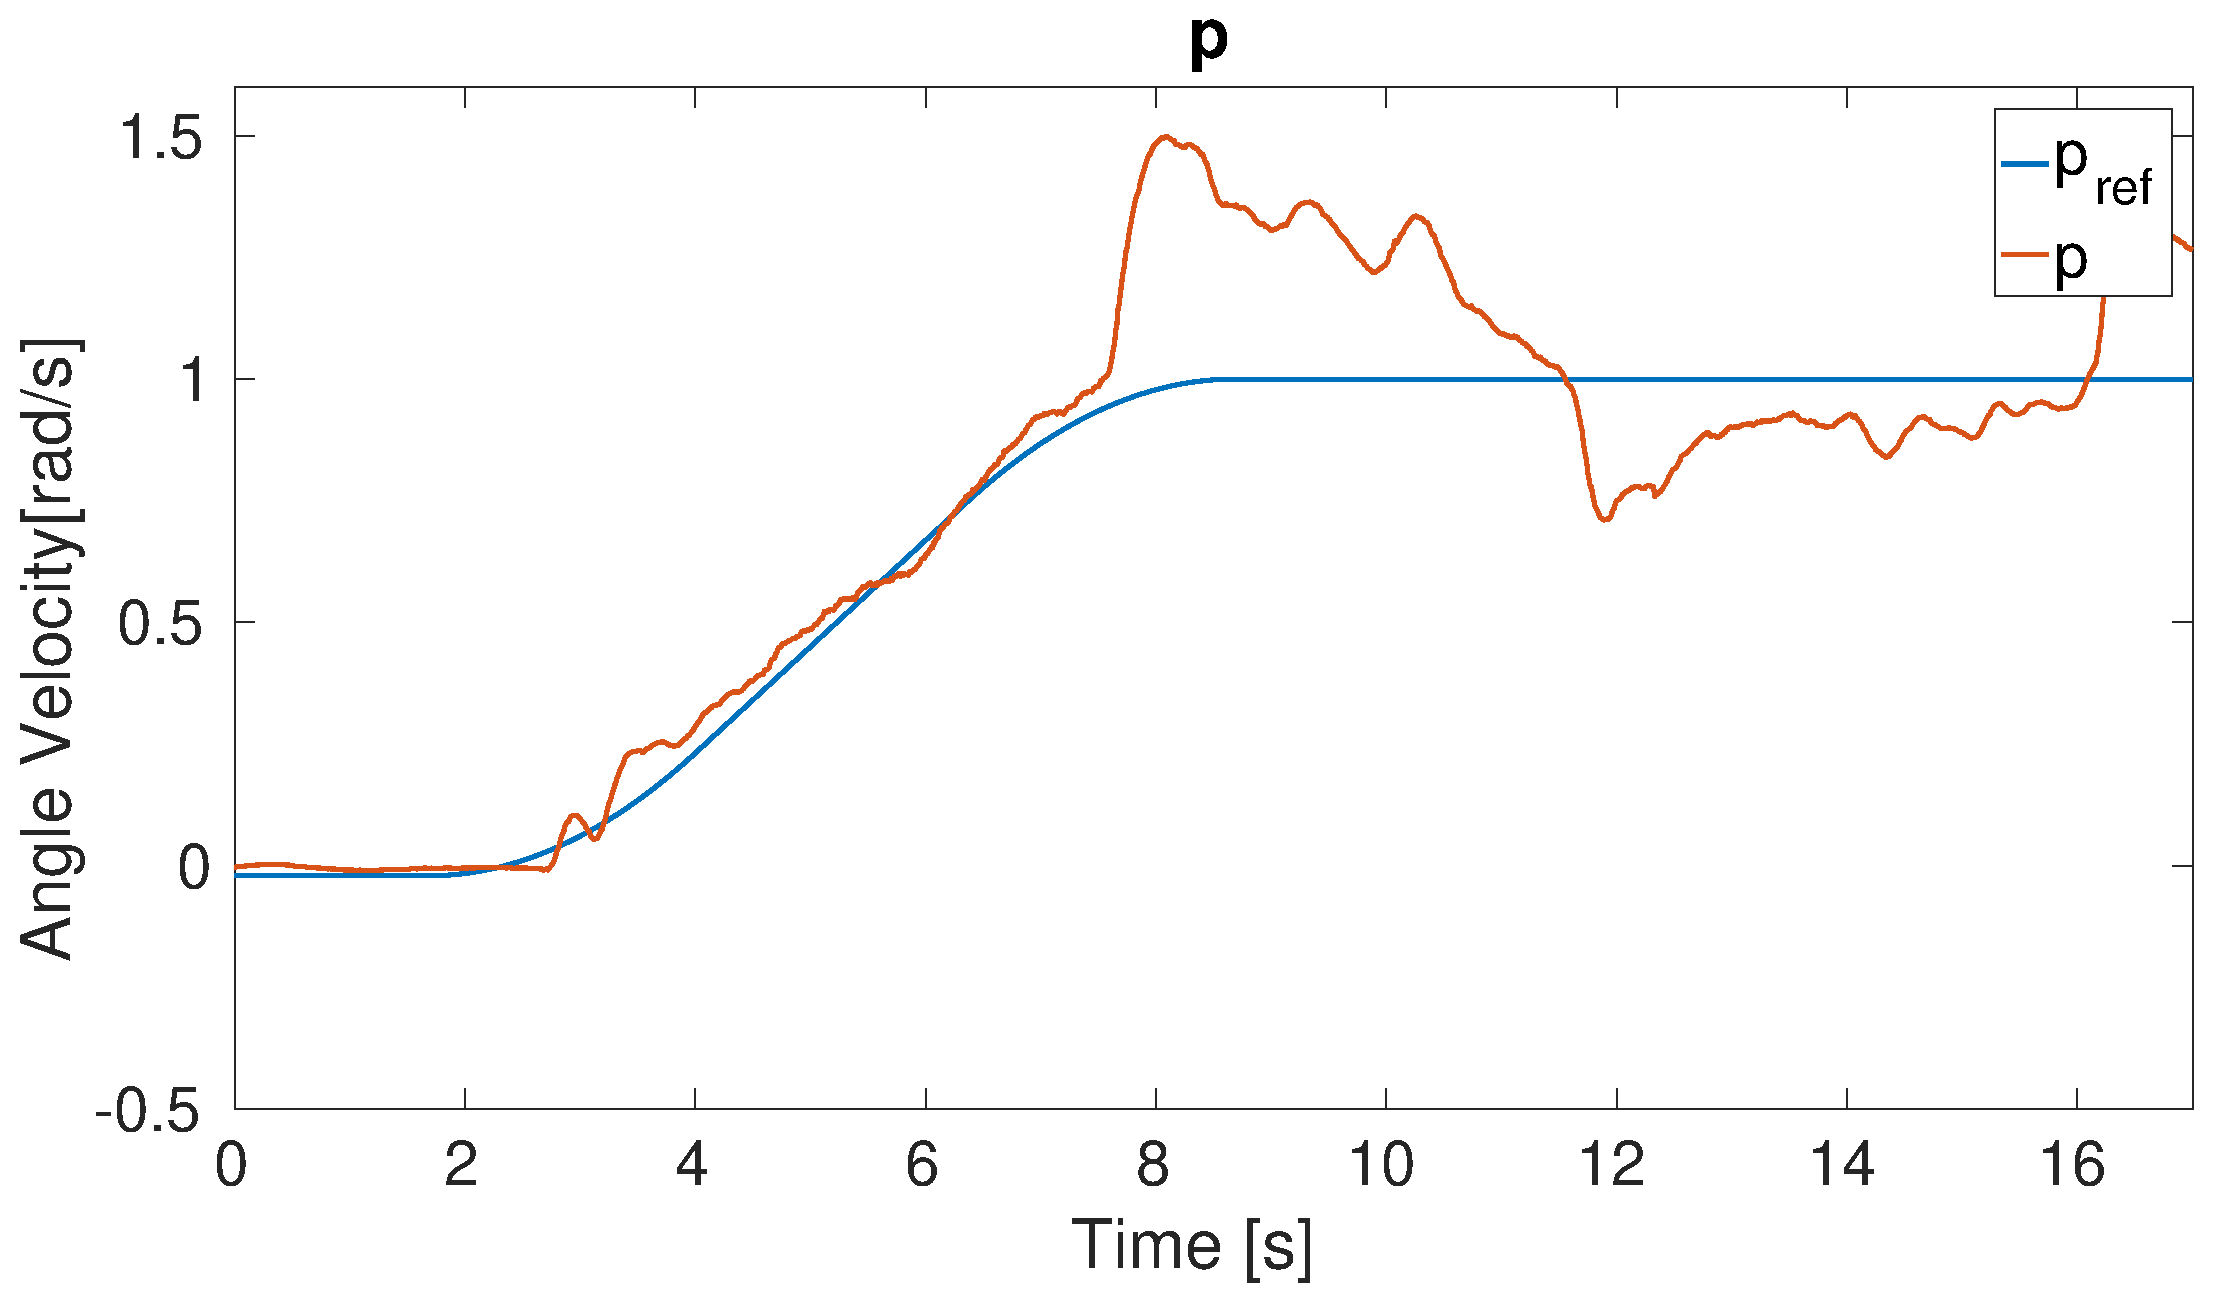
\includegraphics[width=0.4\textwidth]{testStepPs3e10a1}}
  \qquad
  \subfloat[][\label{fig:AppsimStepP} A step applied to the simulated \abbrROV in $\rollVelocity$.]{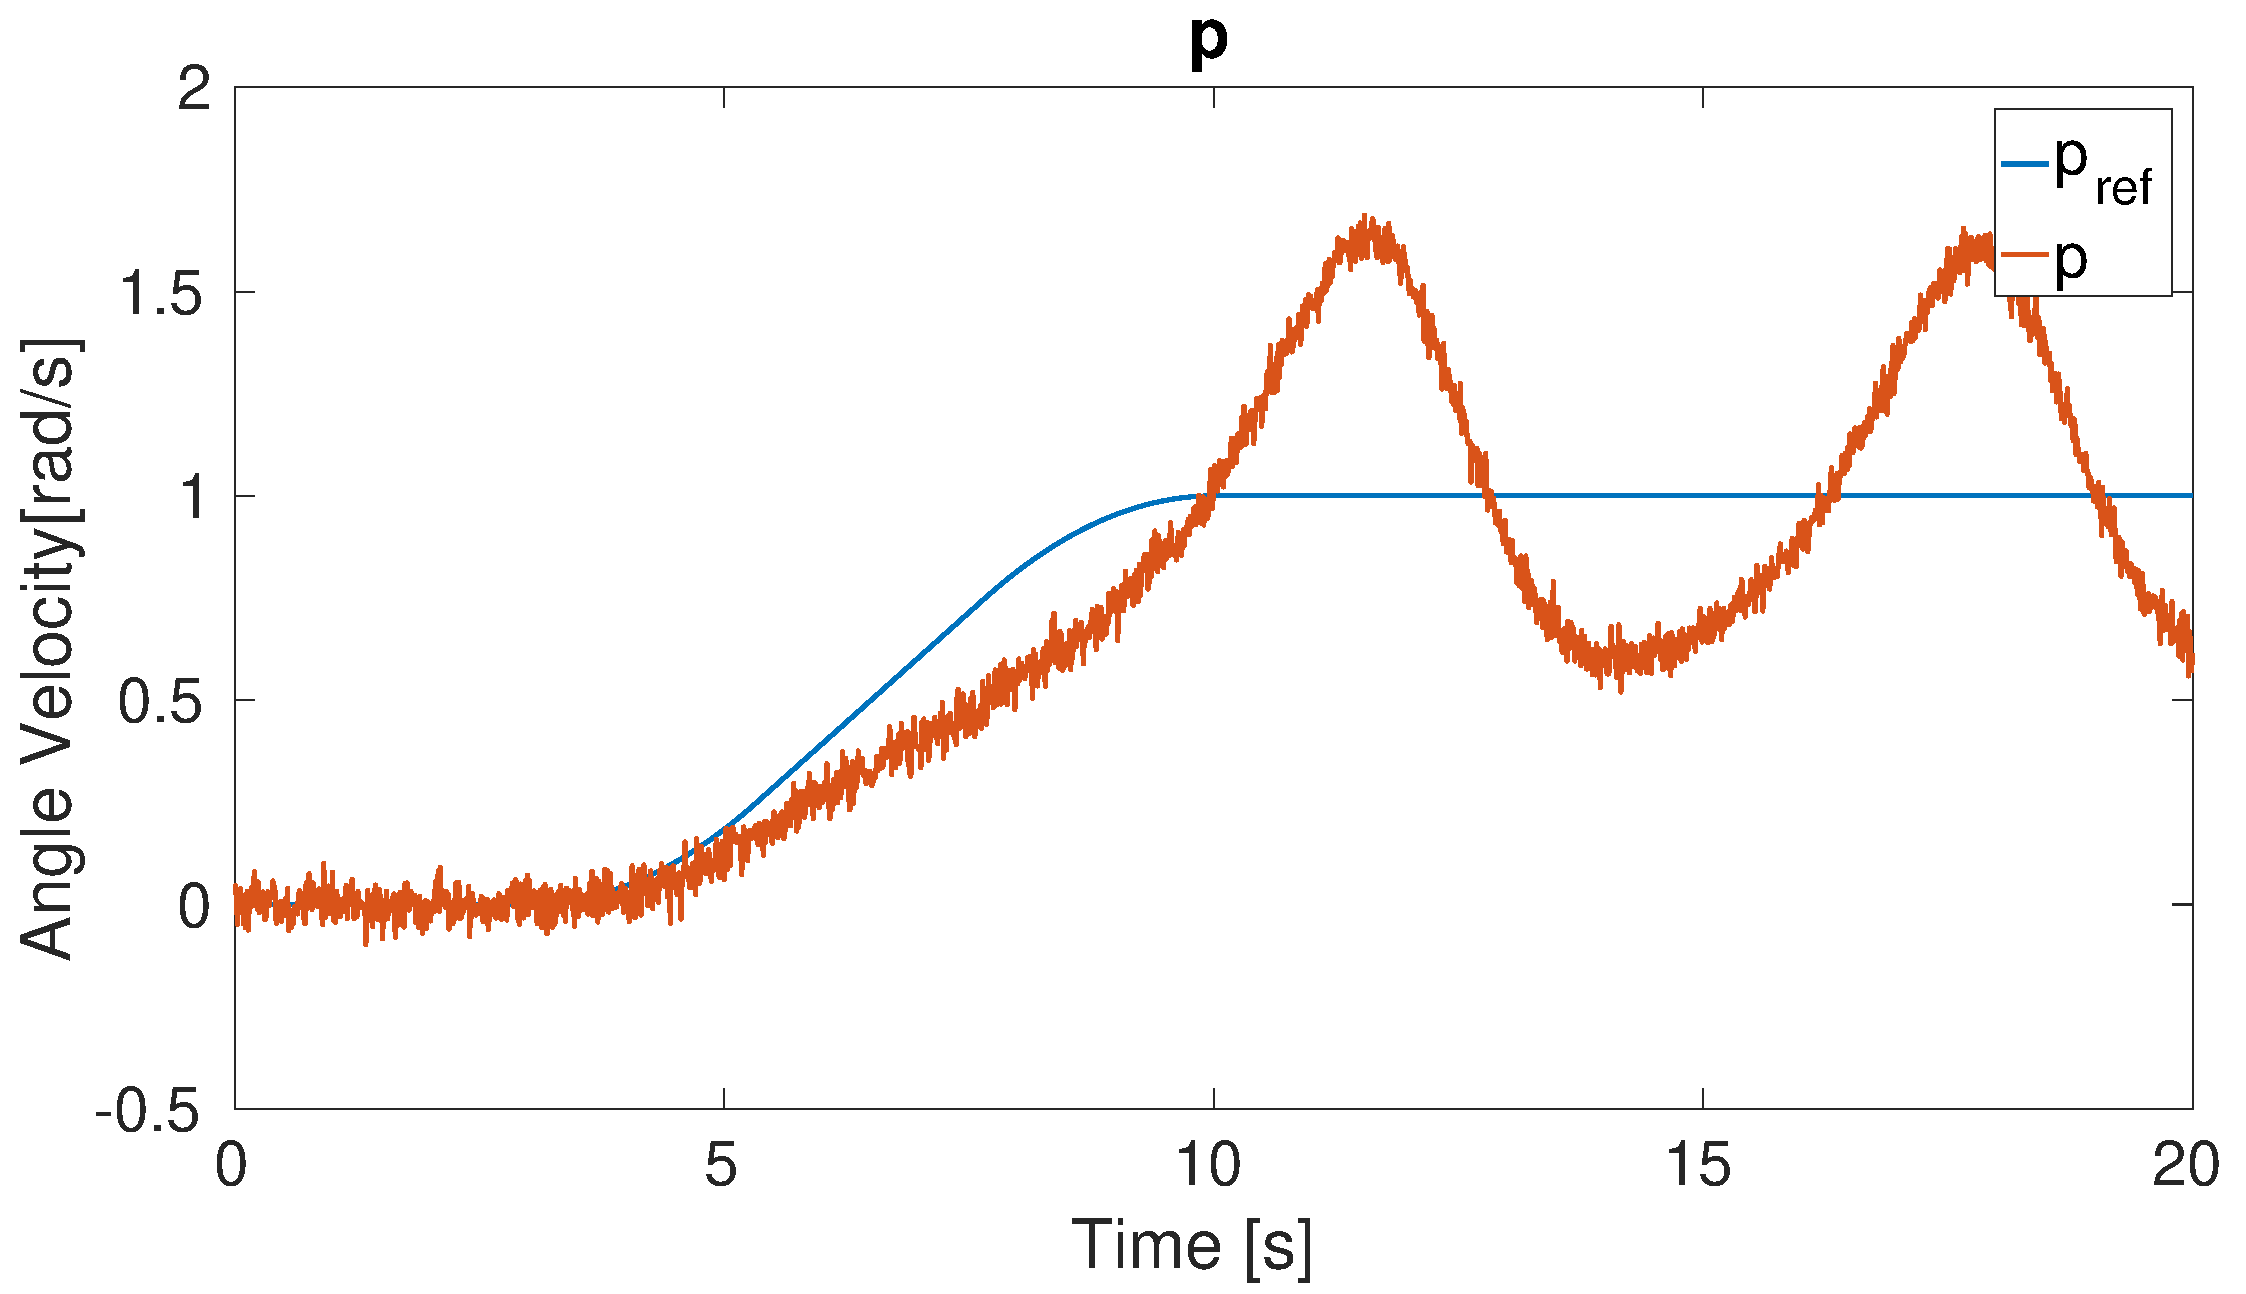
\includegraphics[width=0.4\textwidth]{simStepPs3e10a1}}
  \qquad
  \subfloat[][\label{fig:ApptestStepQ} A smooth step applied in $\pitchVelocity$.]{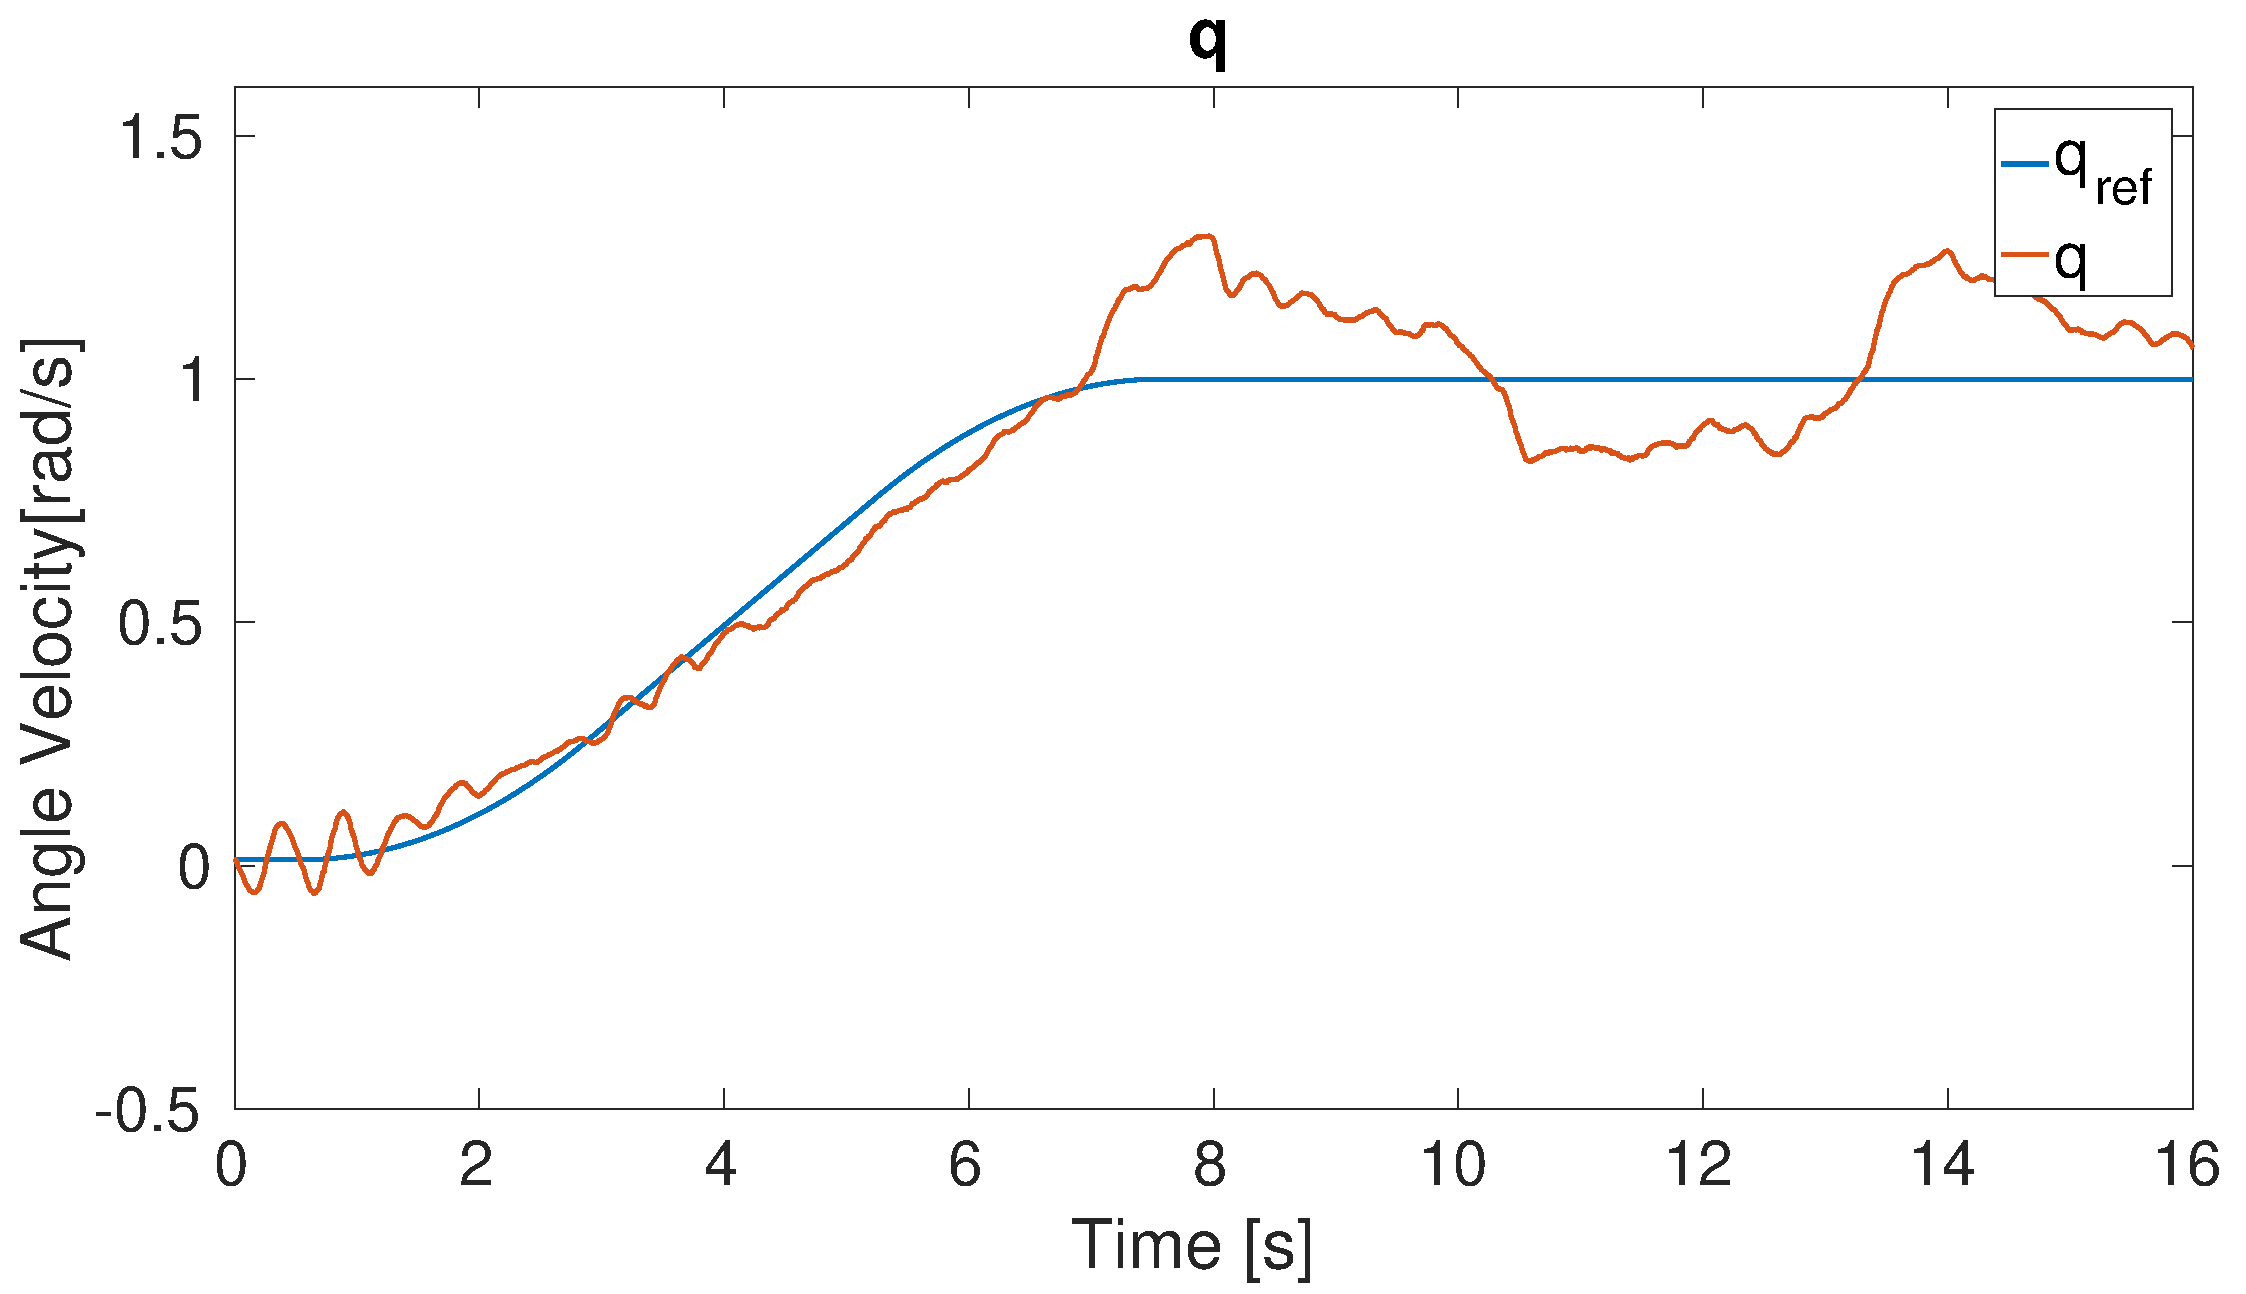
\includegraphics[width=0.4\textwidth]{testStepQs3e10a1}}
  \qquad
  \subfloat[][\label{fig:AppsimStepQ} A step applied to the simulated \abbrROV in $\pitchVelocity$.]{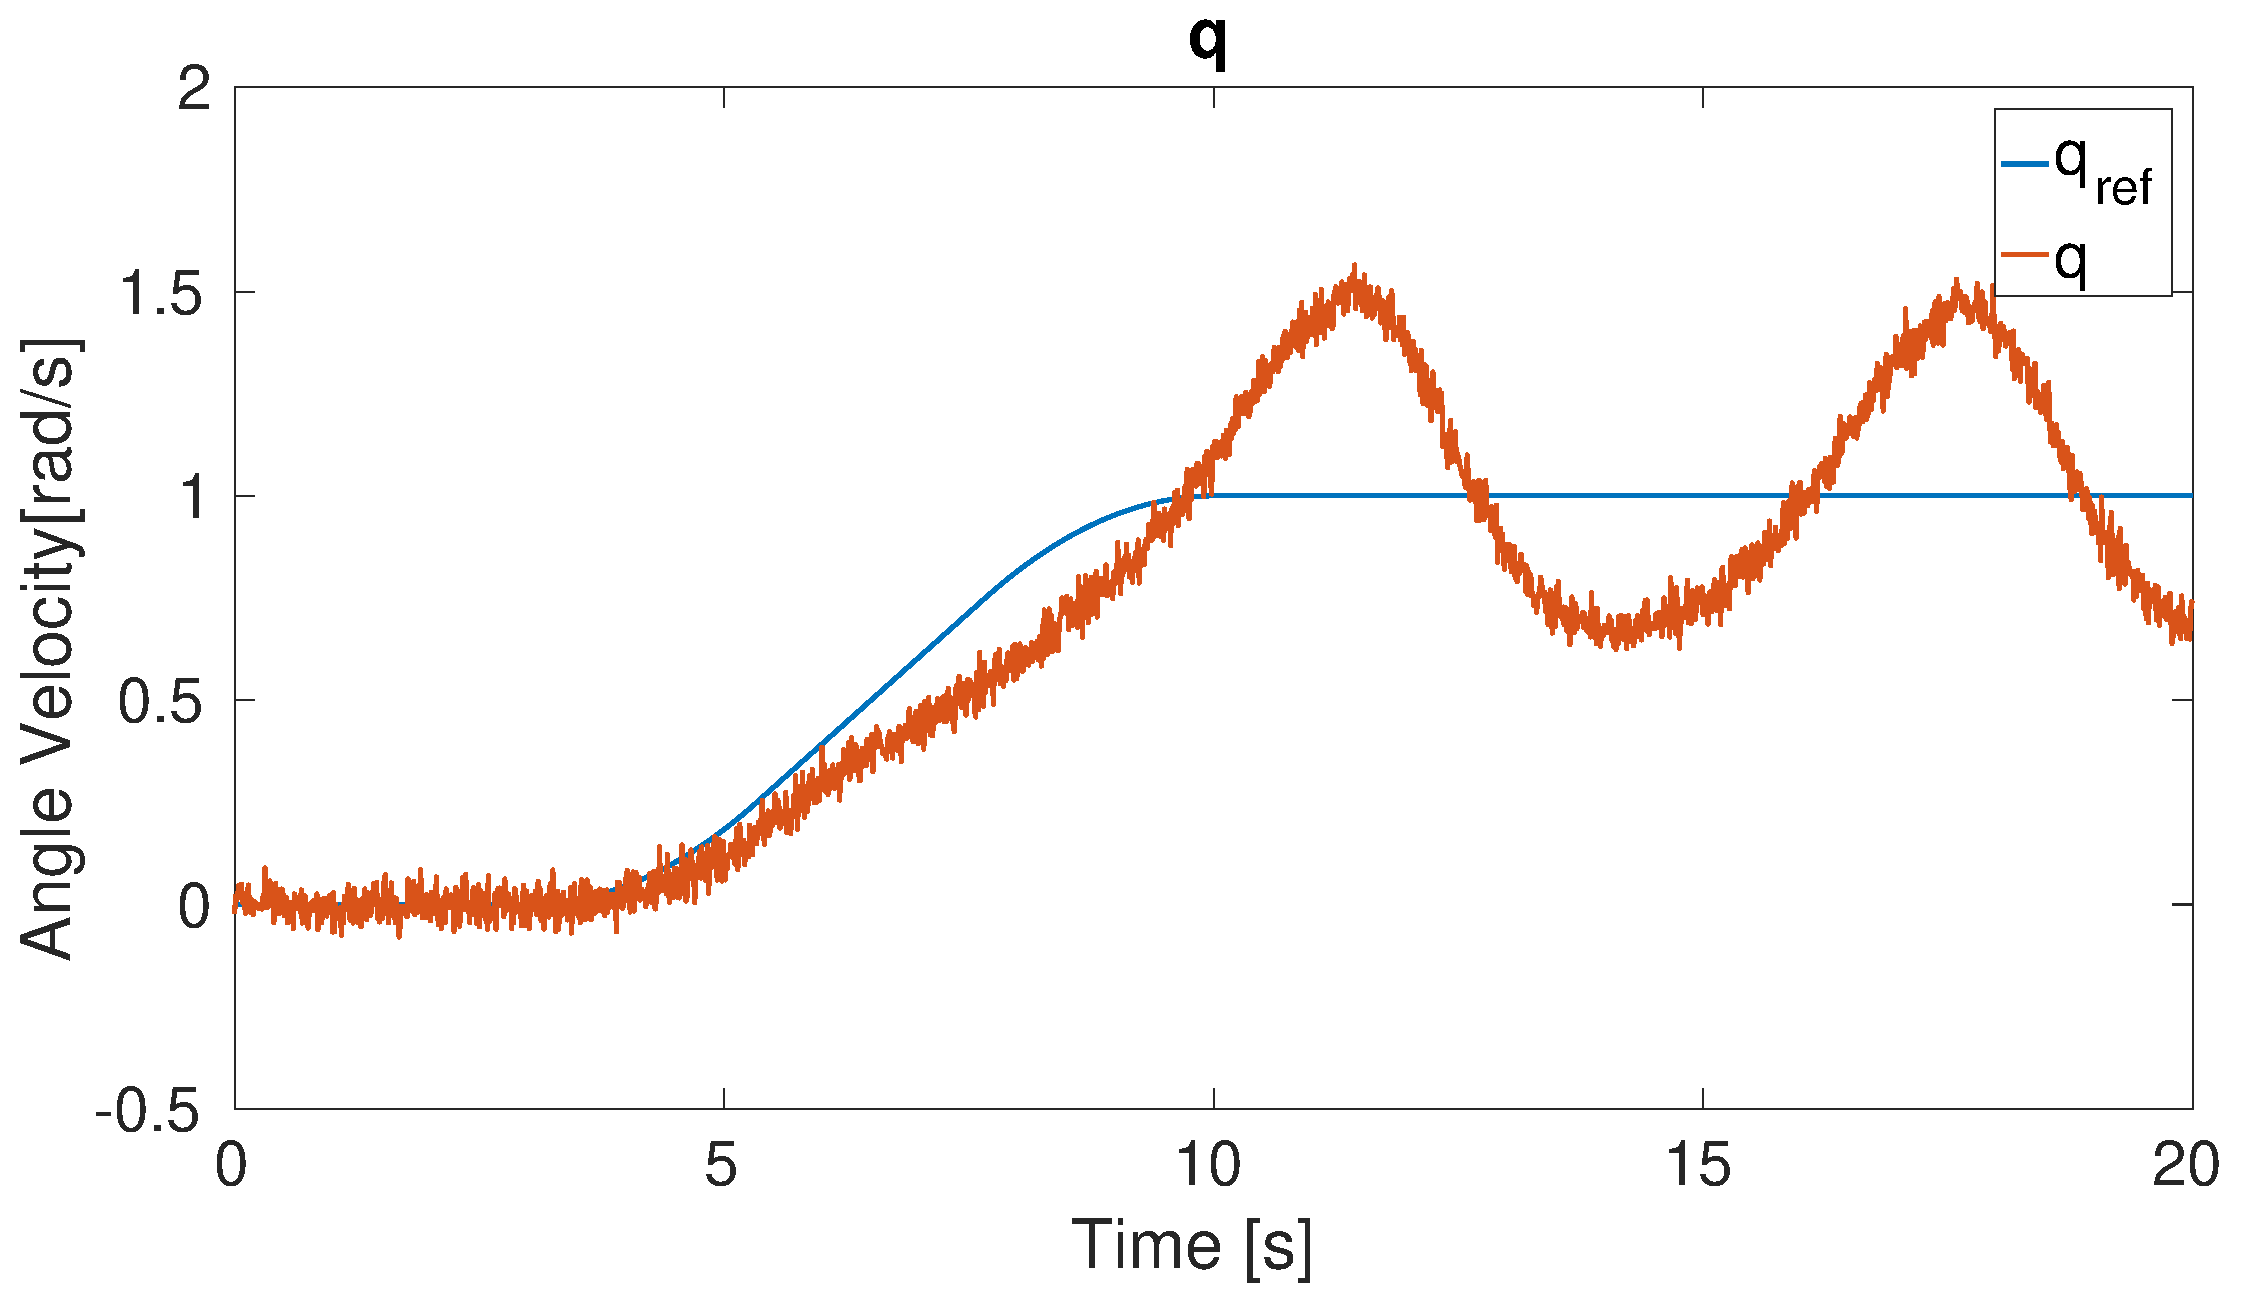
\includegraphics[width=0.4\textwidth]{simStepQs3e10a1}}
  \qquad
  \subfloat[][\label{fig:ApptestStepR} A smooth step applied in $\yawVelocity$.]{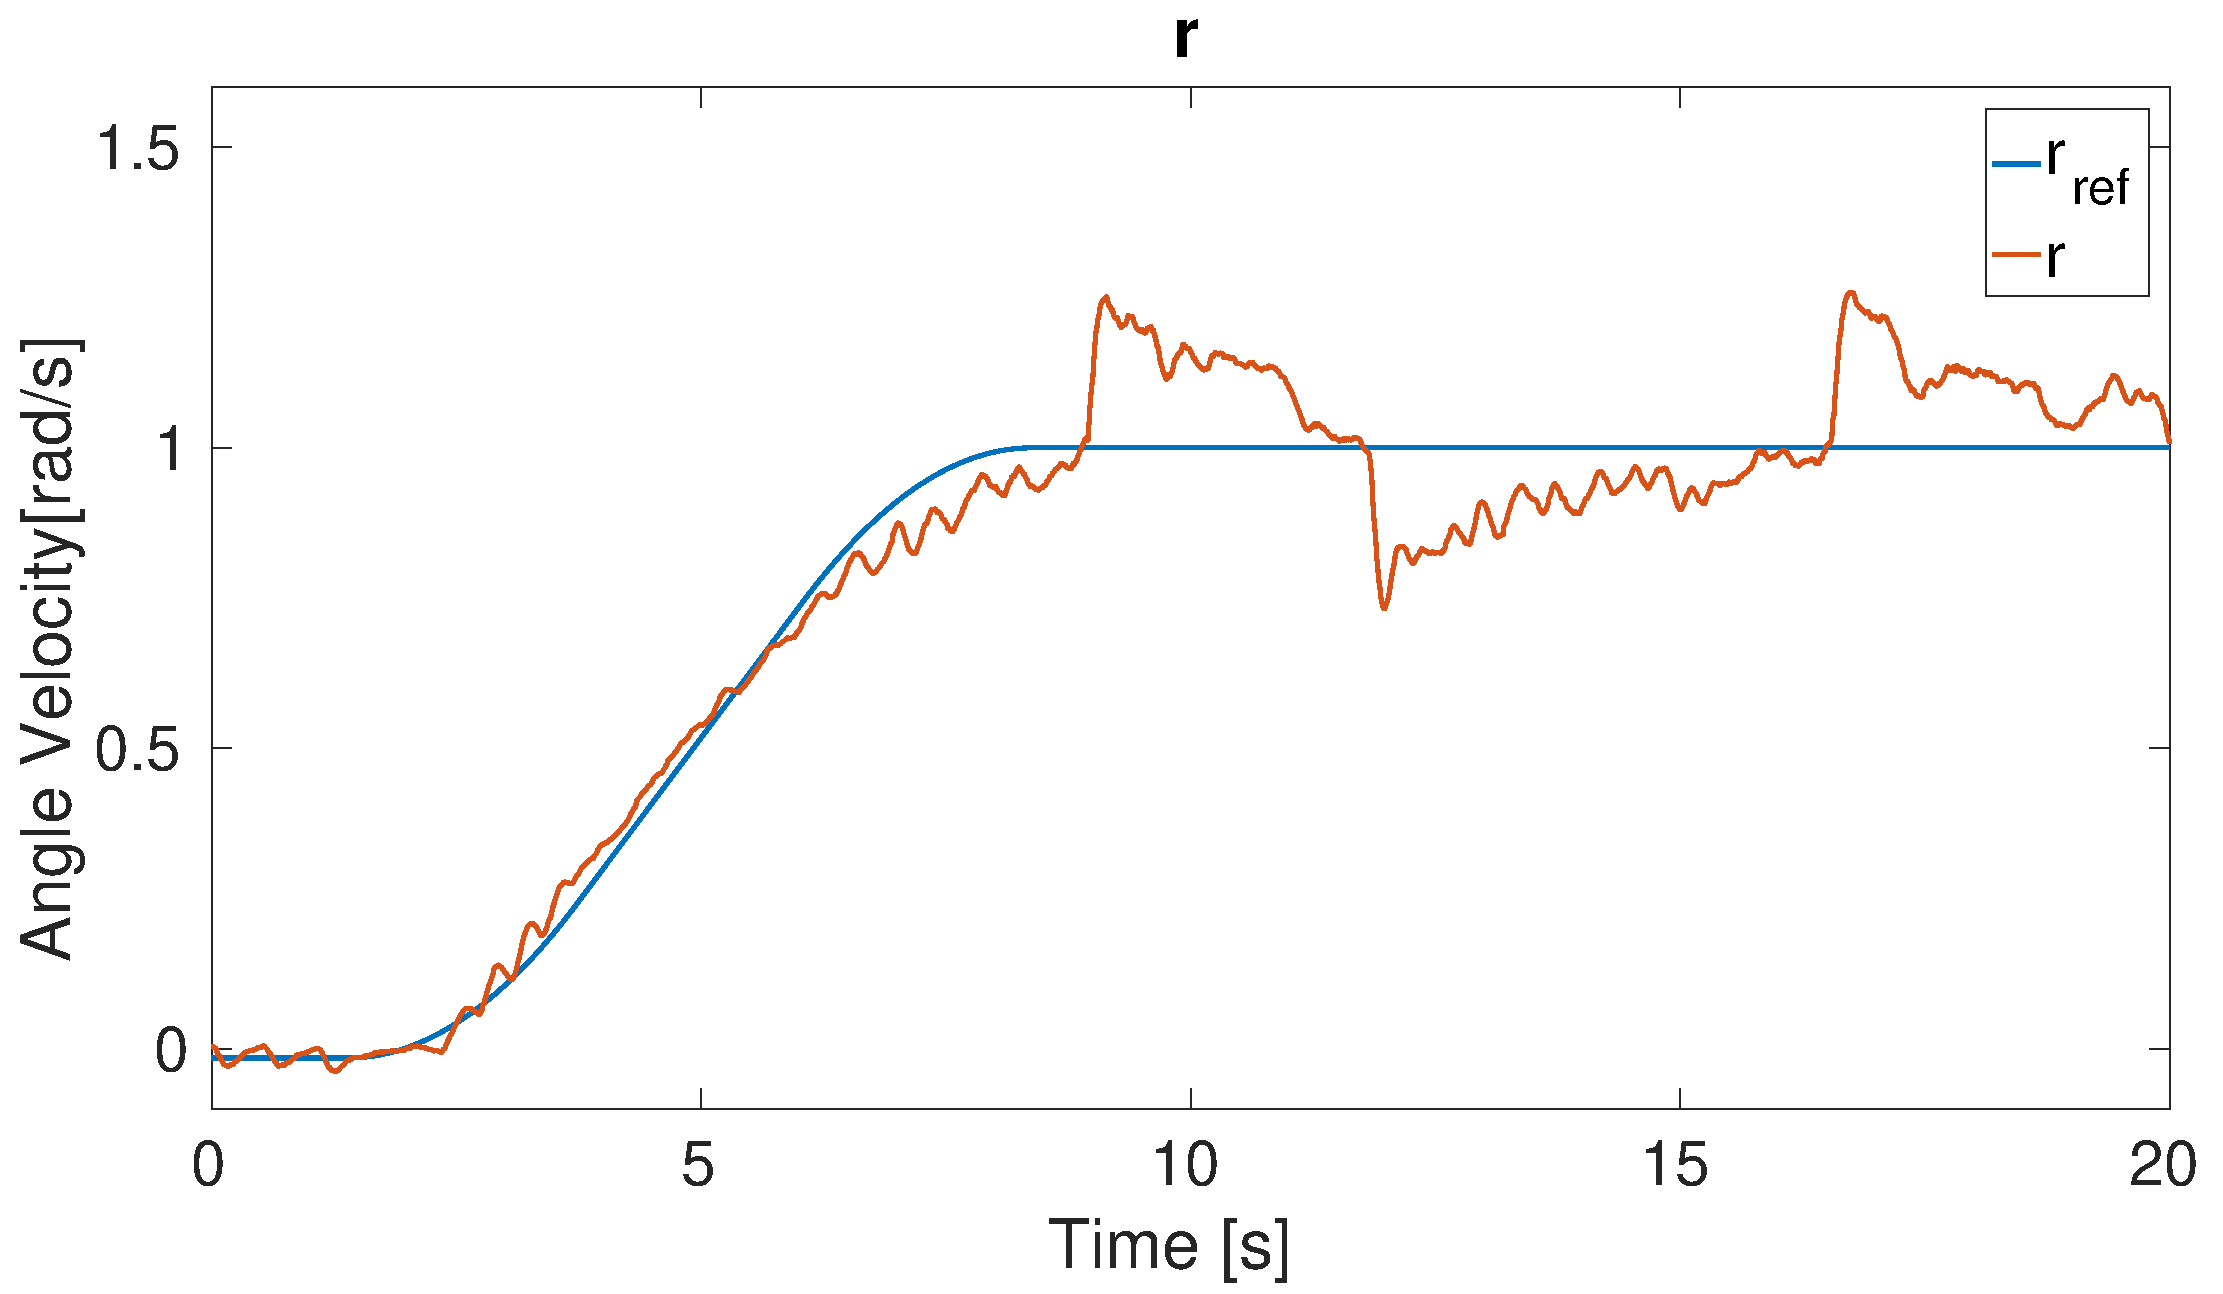
\includegraphics[width=0.4\textwidth]{testStepRs3e10a1}}
  \qquad
  \subfloat[][\label{fig:AppsimStepR} A step applied to the simulated \abbrROV in $\yawVelocity$.]{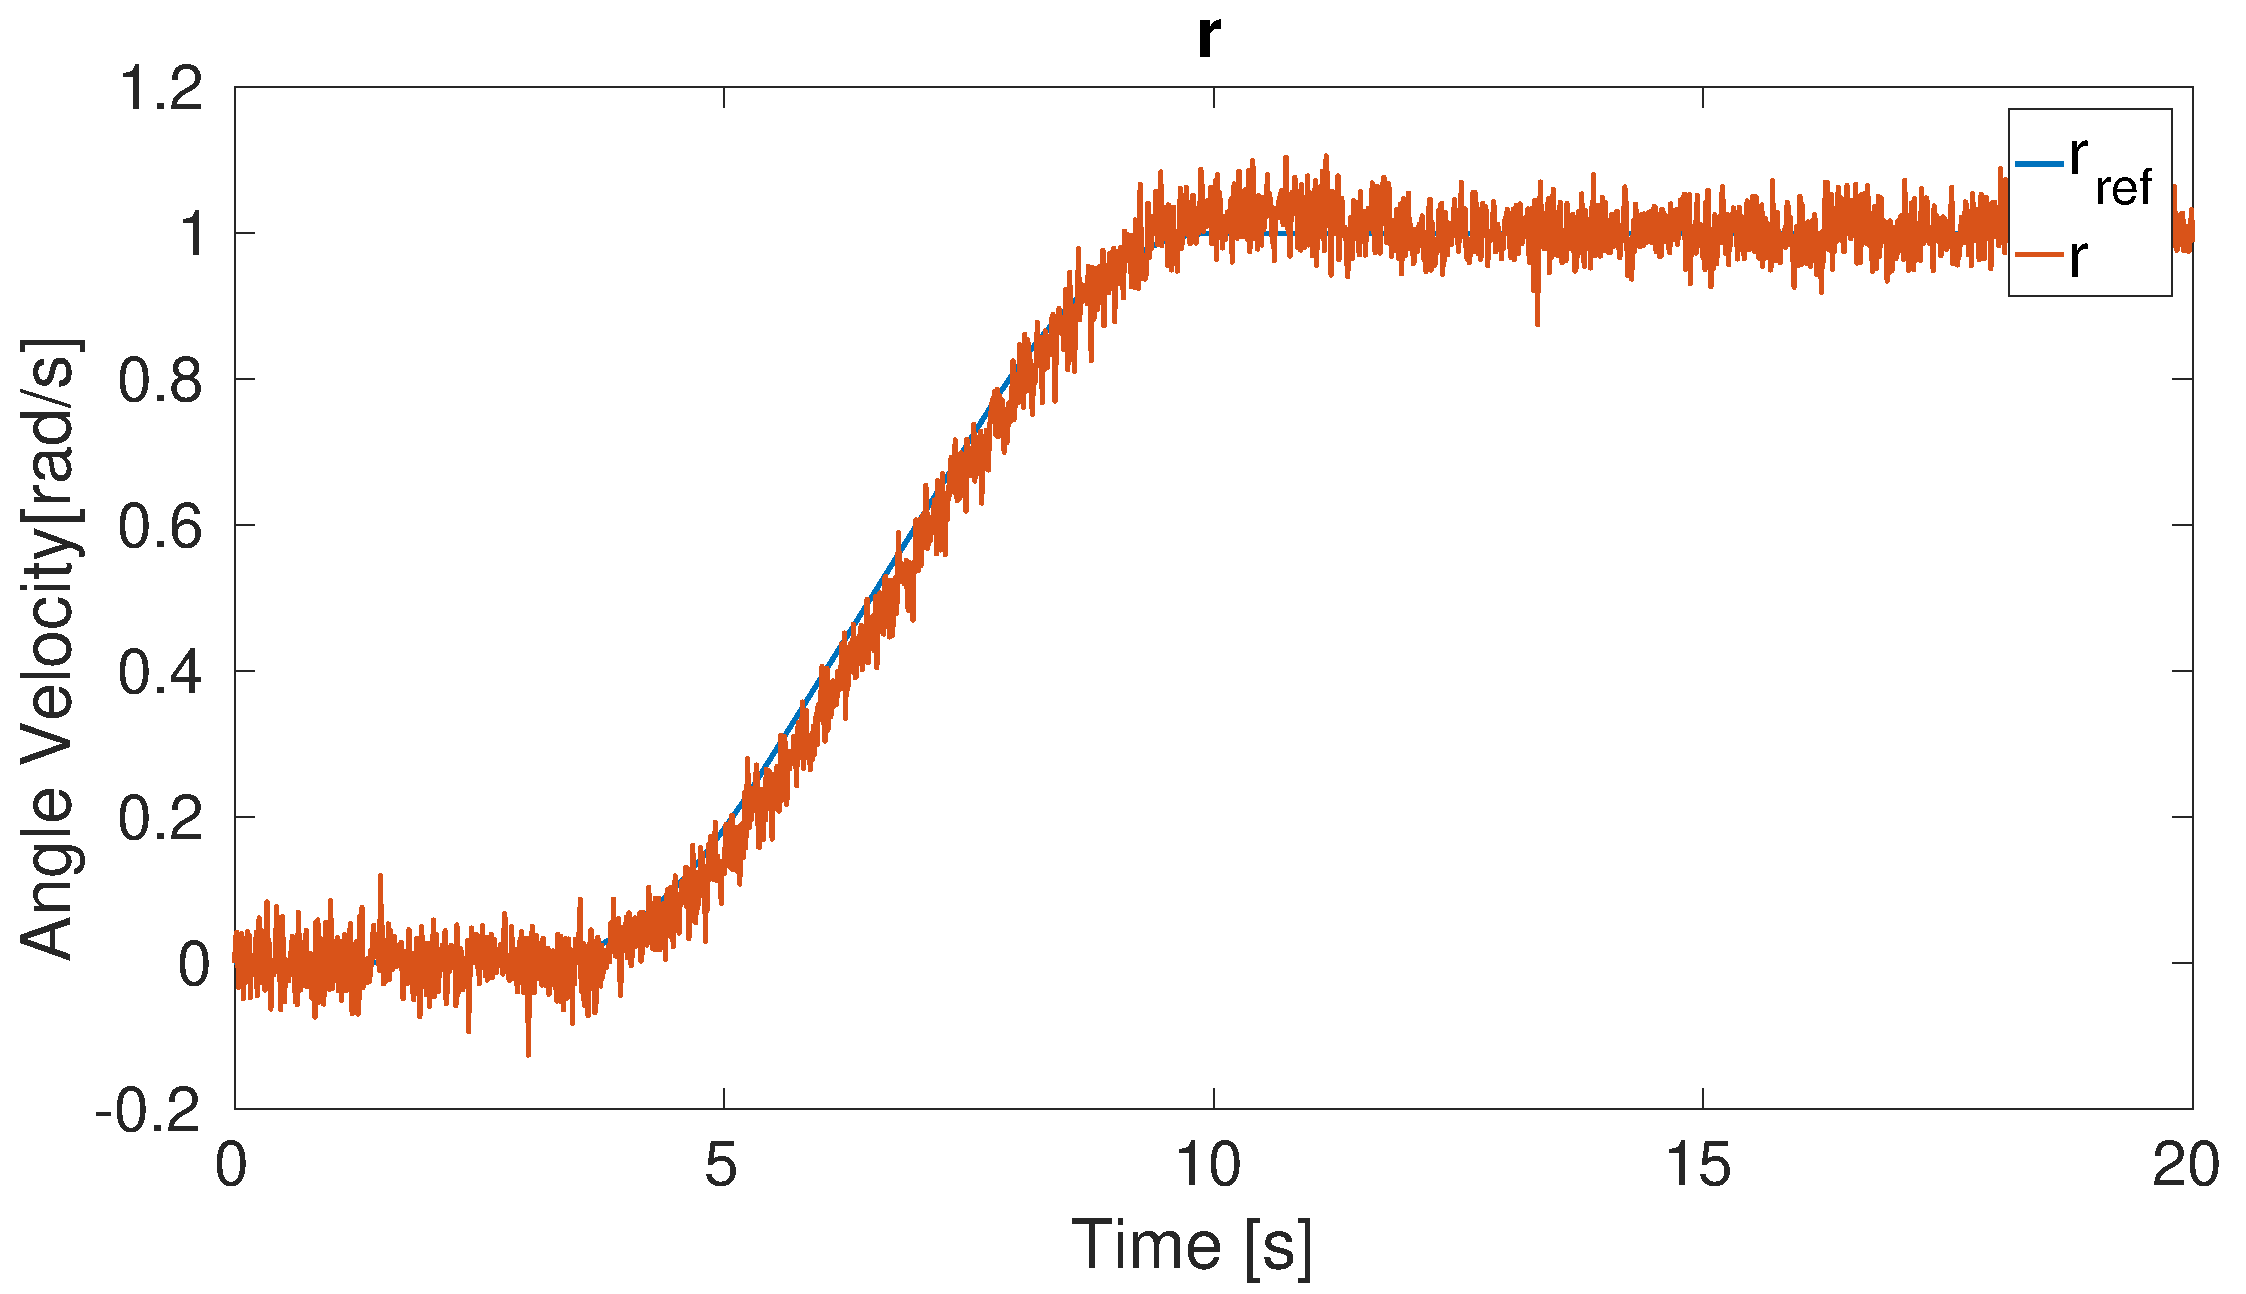
\includegraphics[width=0.4\textwidth]{simStepRs3e10a1}}
   \caption{\label{fig:AppStepRate}%
   A smooth step was applied in one angular velocity at a time while using the rate controller. While a smooth step was applied in one angular velocity the other angular velocities were controlled with the reference zero.}
\end{figure}

\begin{figure}
\centering
  \subfloat[][\label{fig:ApptestStepAllPRate} A smooth step applied in $\rollVelocity$.]{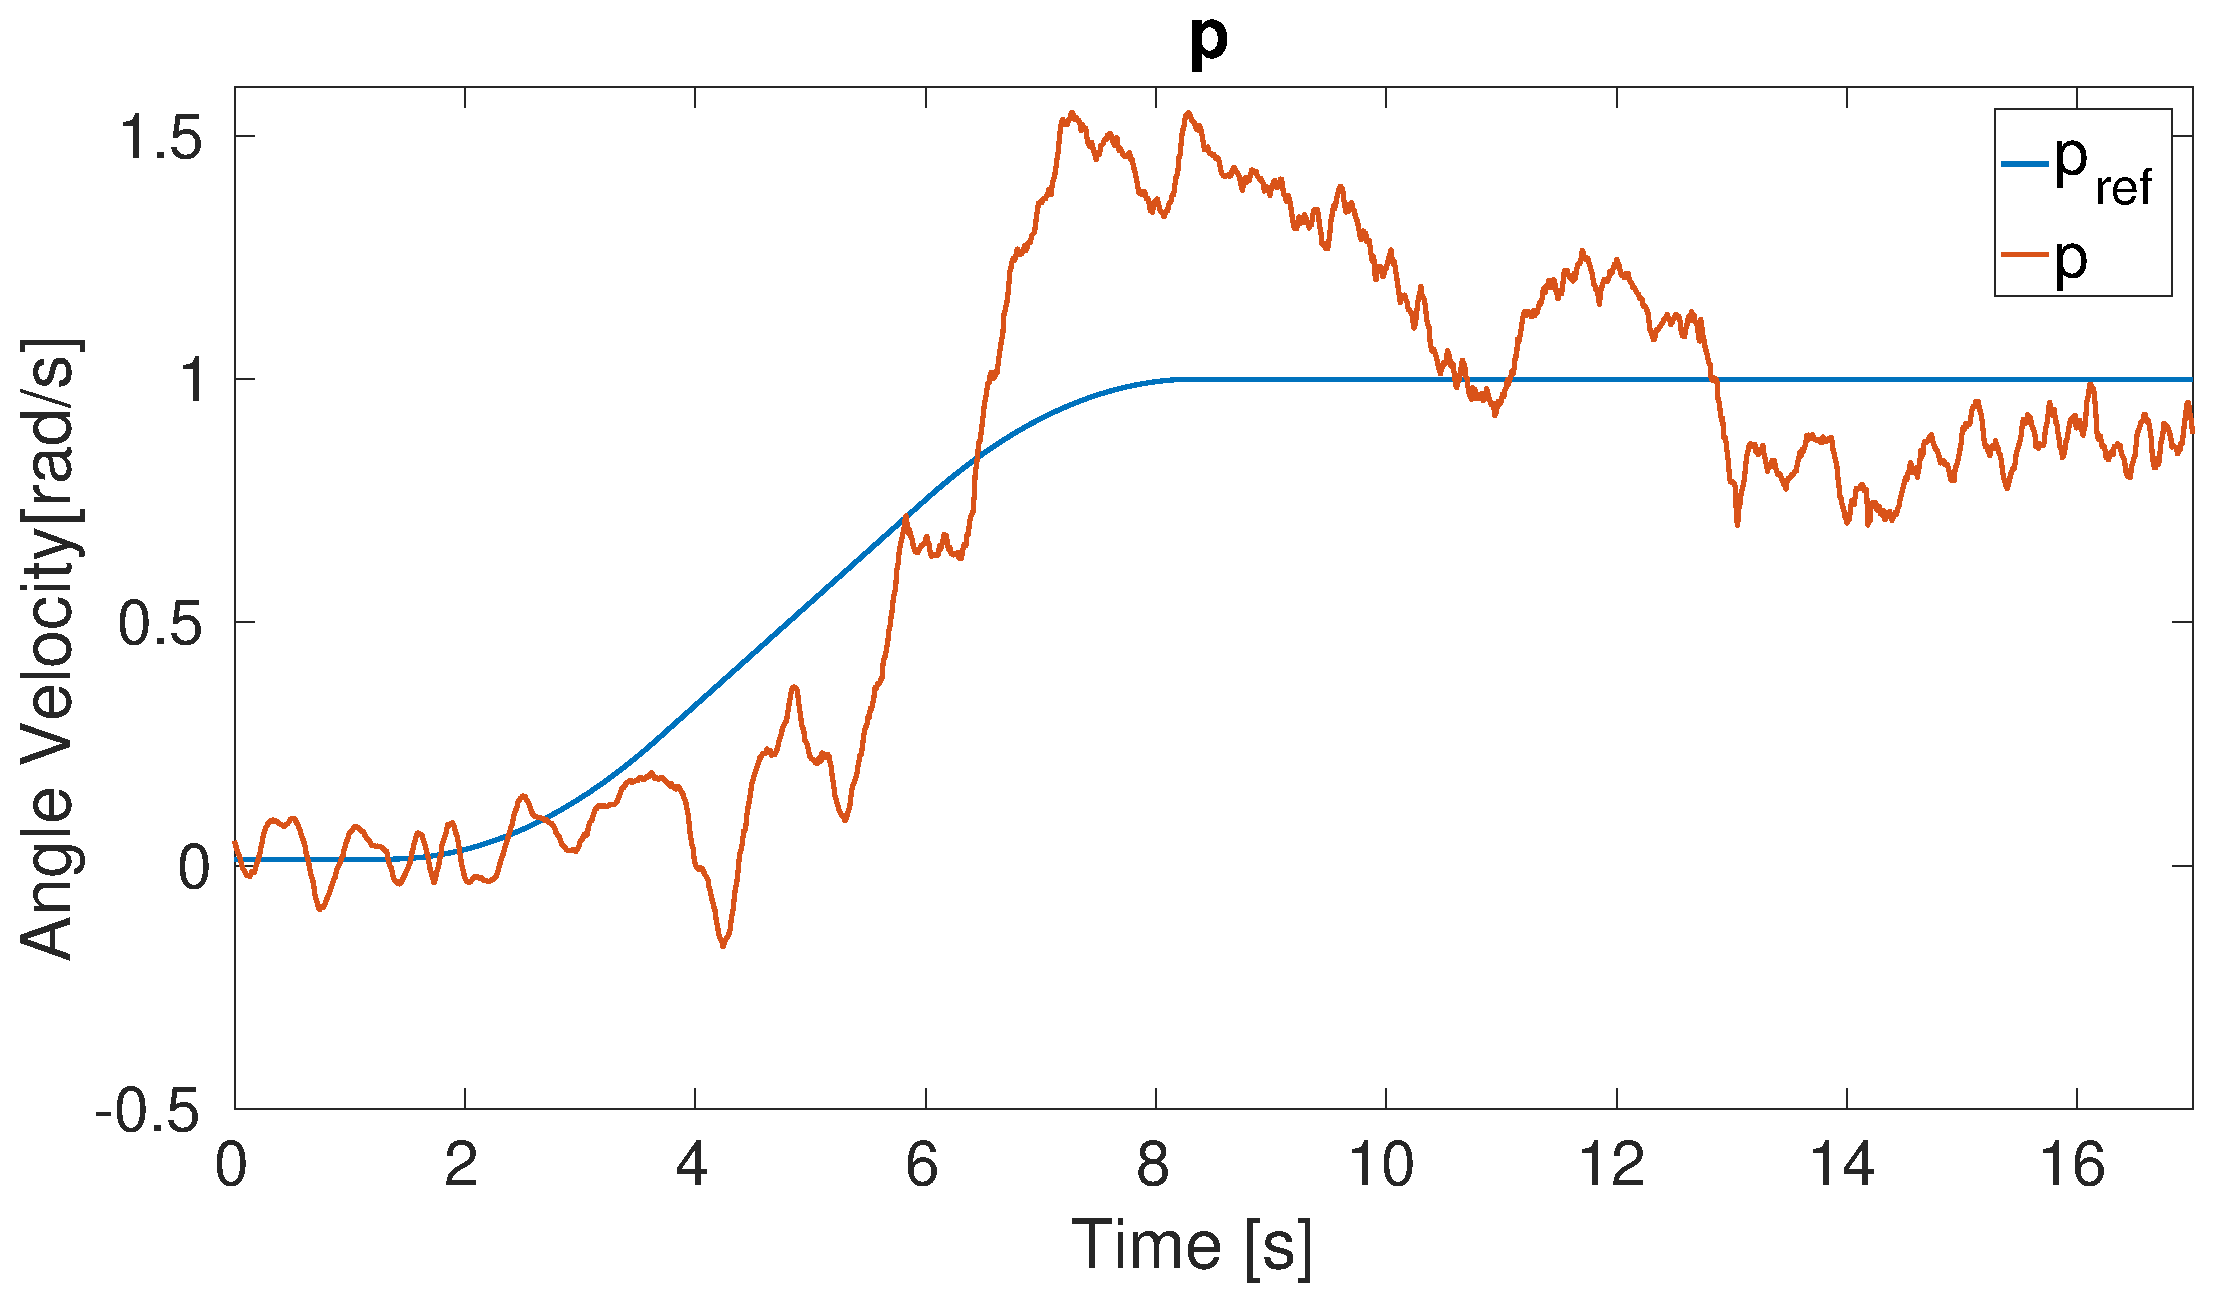
\includegraphics[width=0.4\textwidth]{testStepAllPs3e10a1}}
  \qquad
  \subfloat[][\label{fig:AppsimStepAllPRate} A step applied to the simulated \abbrROV in $\rollVelocity$.]{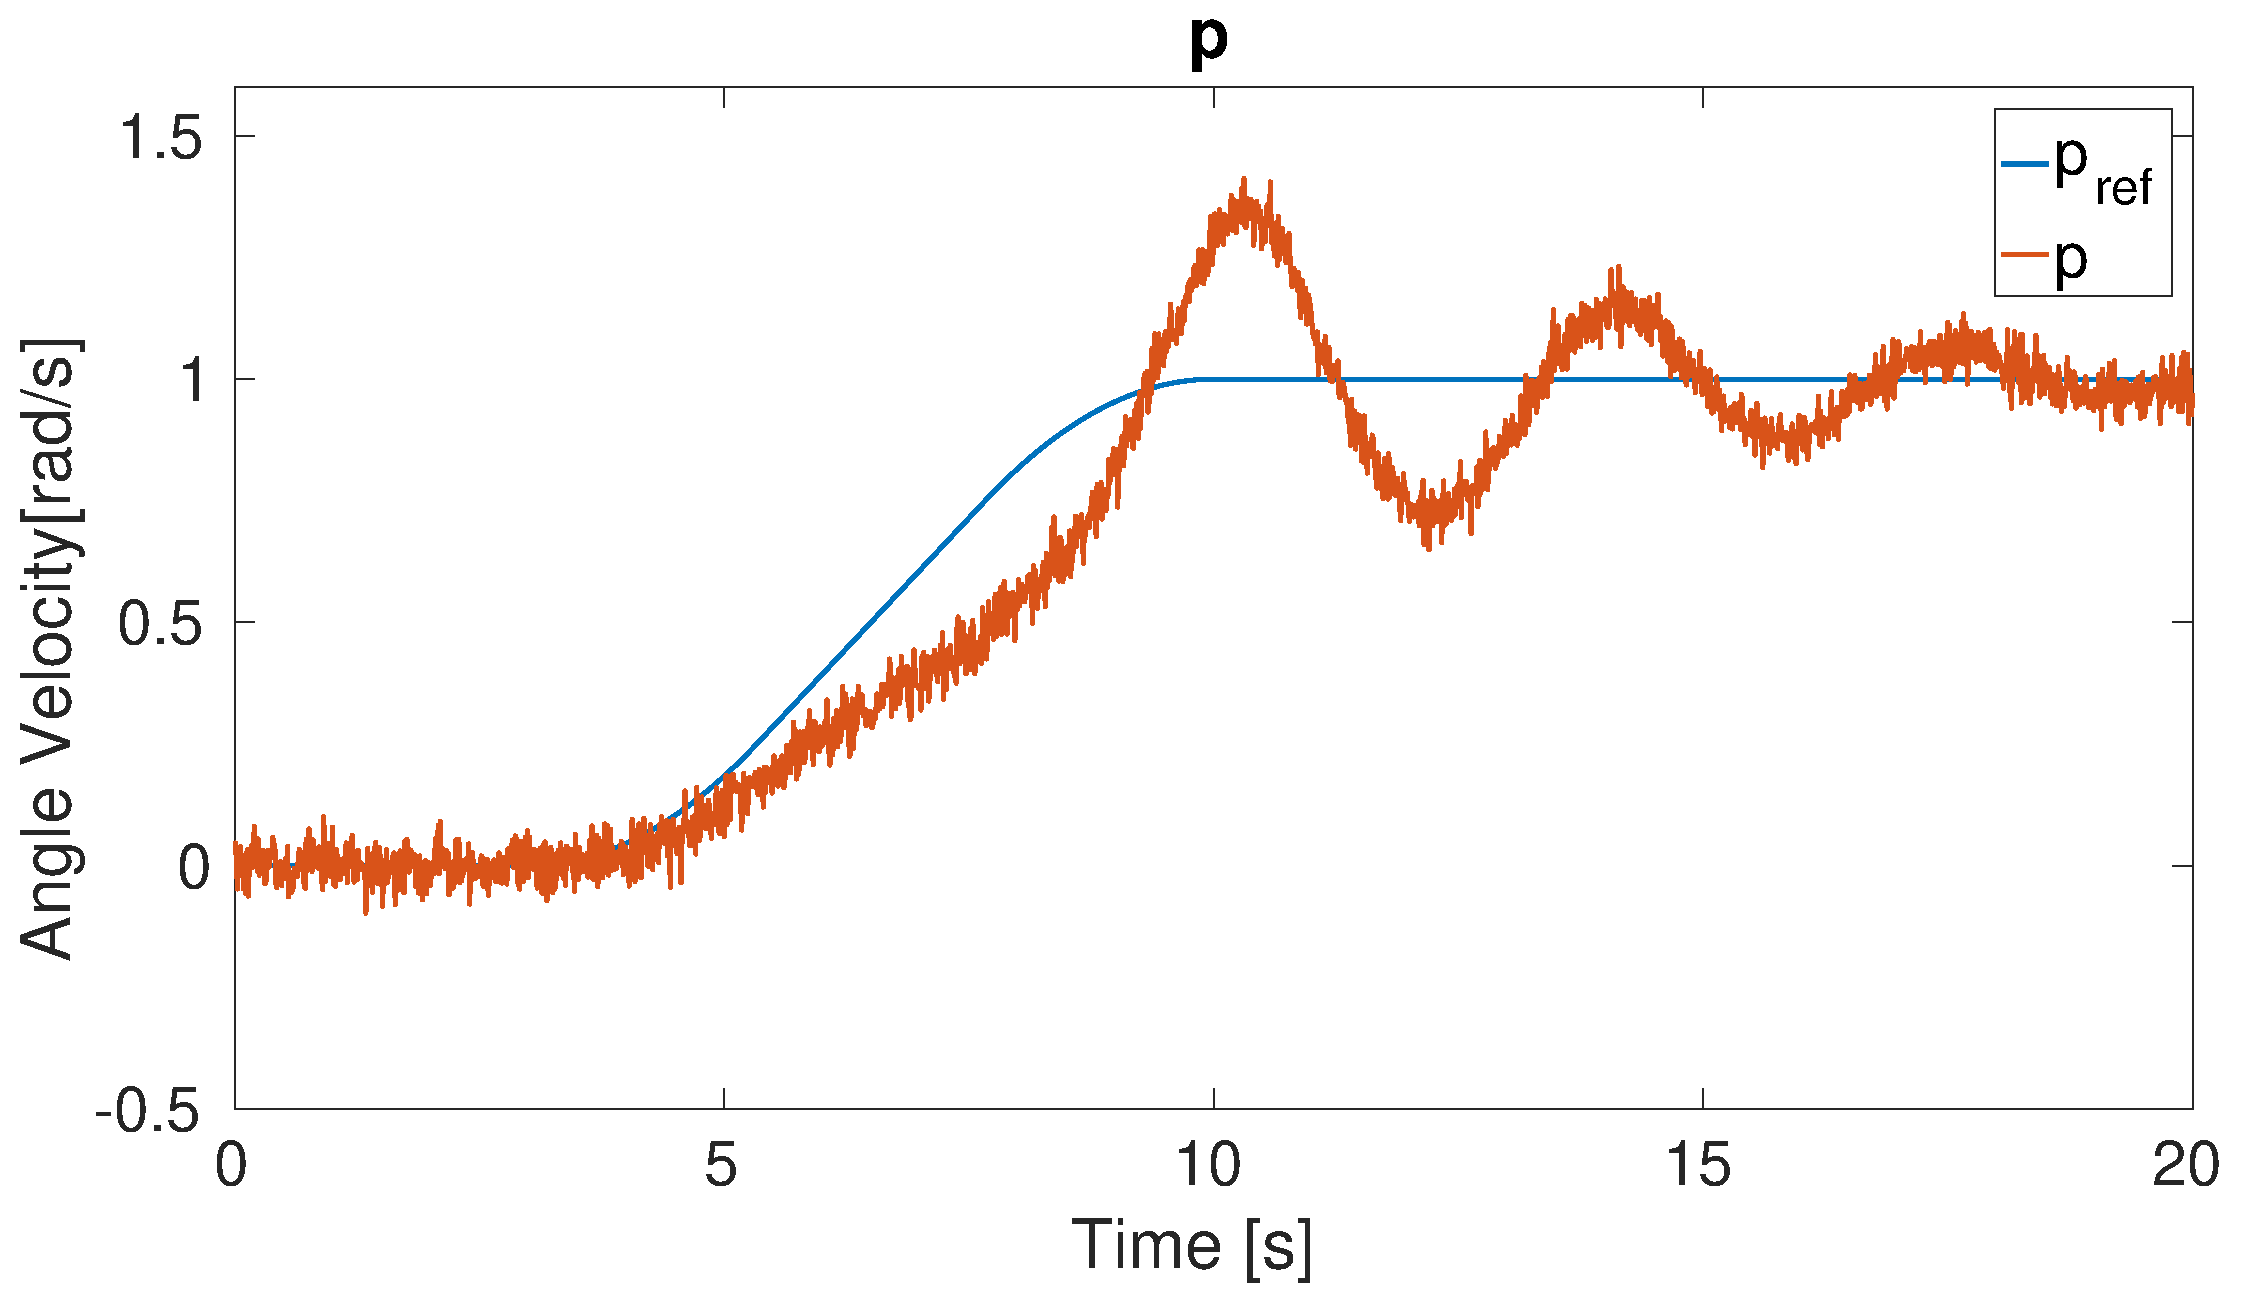
\includegraphics[width=0.4\textwidth]{simStepAllPs3e10a1}}
  \qquad
  \subfloat[][\label{fig:ApptestStepAllQRate} A smooth step applied in $\pitchVelocity$.]{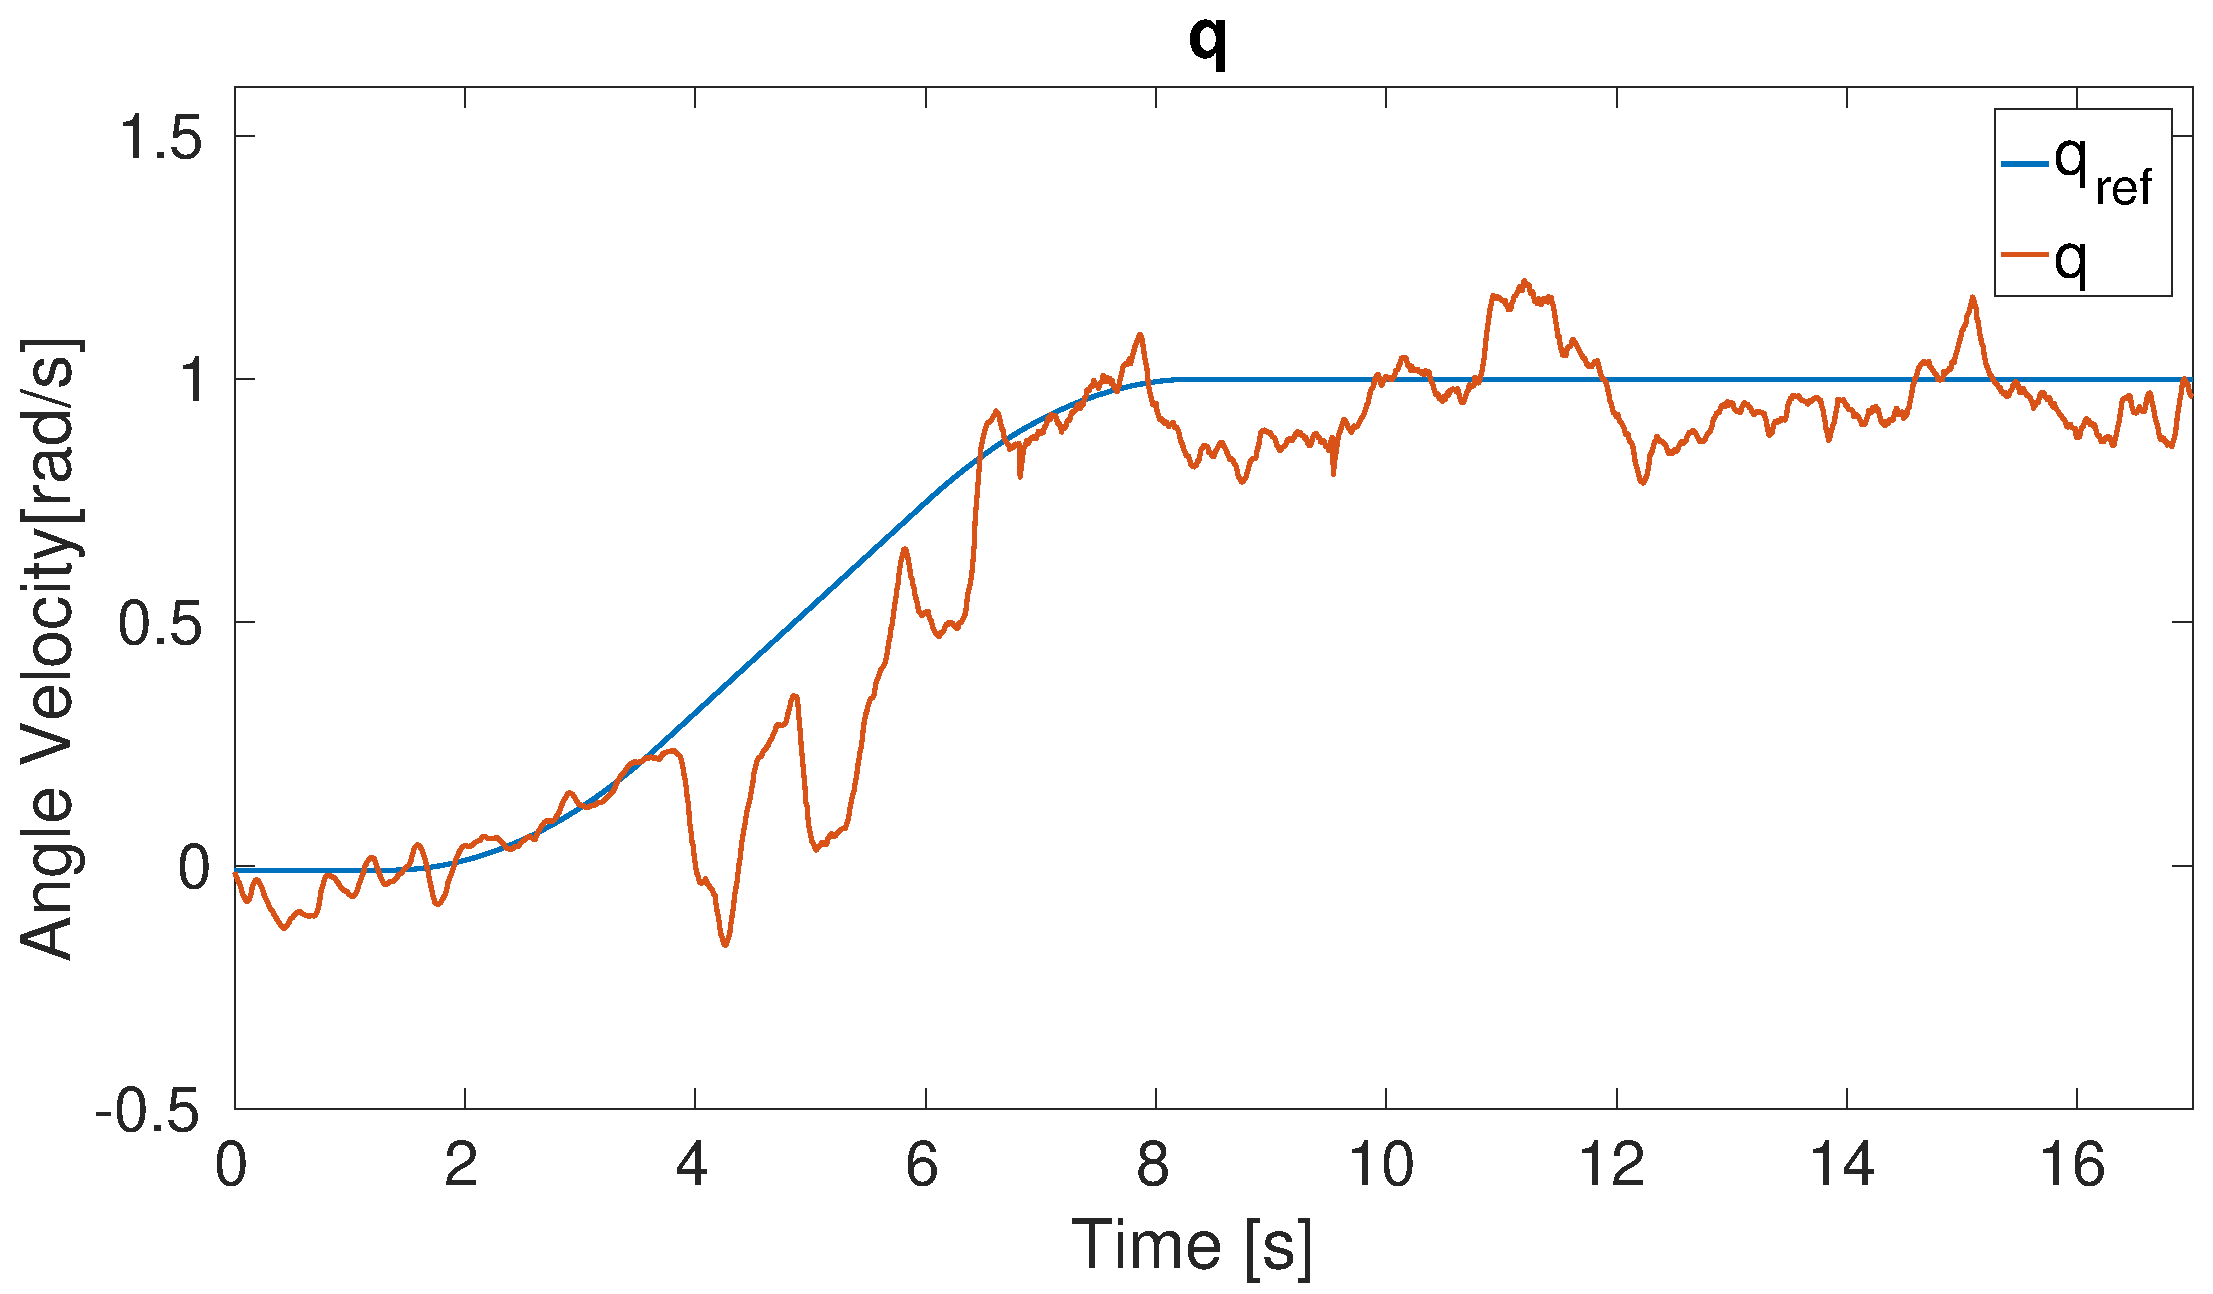
\includegraphics[width=0.4\textwidth]{testStepAllQs3e10a1}}
  \qquad
  \subfloat[][\label{fig:AppsimStepAllQRate} A step applied to the simulated \abbrROV in $\pitchVelocity$.]{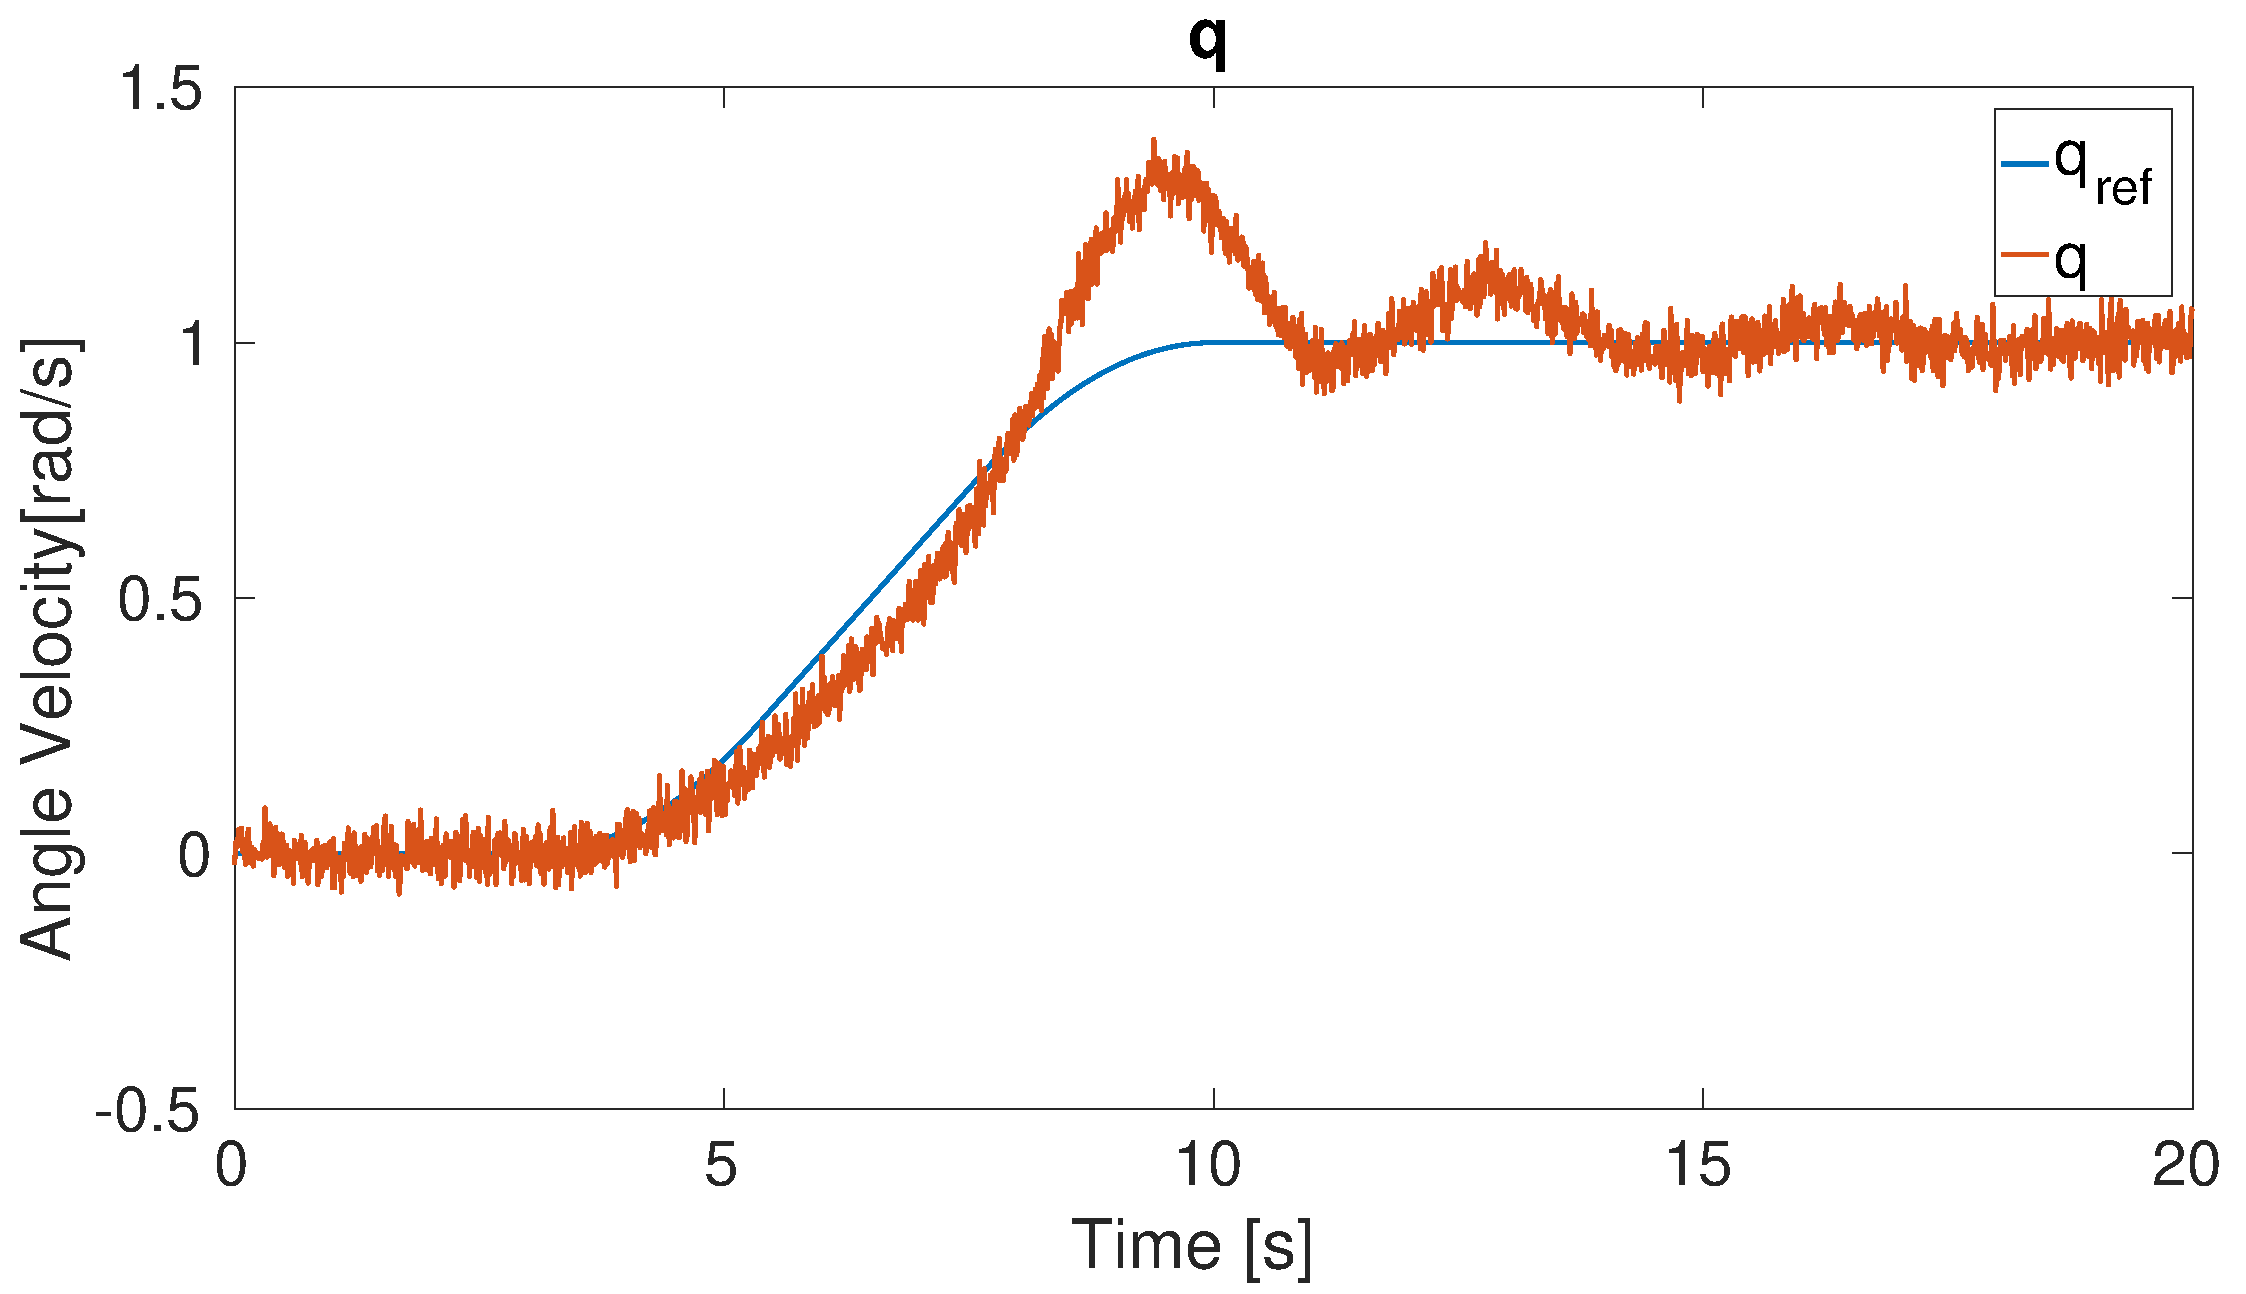
\includegraphics[width=0.4\textwidth]{simStepAllQs3e10a1}}
  \qquad
  \subfloat[][\label{fig:ApptestStepAllRRate} A smooth step applied in $\yawVelocity$.]{\includegraphics[width=0.4\textwidth]{testStepAllRs3e10a1}}
  \qquad
  \subfloat[][\label{fig:AppsimStepAllRRate} A step applied to the simulated \abbrROV in $\yawVelocity$.]{\includegraphics[width=0.4\textwidth]{simStepAllRs3e10a1}}
  \caption{\label{fig:AppStepAllRate}% 
  Smooth steps were applied in all angular velocities at the same time while using the rate controller.}
\end{figure}

\begin{figure}[tbp]
  \centering
  \subfloat[][\label{fig:ApptestSinP} A sine signal with amplitude $1$ and frequency $0.5\hertz$ applied in $\rollVelocity$.]{\includegraphics[width=0.4\textwidth]{testSinPA1}}
  \qquad
  \subfloat[][\label{fig:AppsimSinP} A sine signal with amplitude $1$ and frequency $0.5\hertz$ applied to the simulated \abbrROV in $\rollVelocity$.]{\includegraphics[width=0.4\textwidth]{simSinPA1}}
  \qquad
  \subfloat[][\label{fig:ApptestSinQ} A sine signal with amplitude $1$ and frequency $0.5\hertz$ applied in $\pitchVelocity$.]{\includegraphics[width=0.4\textwidth]{testSinQA1}}
  \qquad
  \subfloat[][\label{fig:AppsimSinQ} A sine signal with amplitude $1$ and frequency $0.5\hertz$ applied to the simulated \abbrROV in $\pitchVelocity$.]{\includegraphics[width=0.4\textwidth]{simSinQA1}}
  \qquad
  \subfloat[][\label{fig:ApptestSinR} A sine signal with amplitude $1$ and frequency $0.5\hertz$ applied in $\yawVelocity$.]{\includegraphics[width=0.4\textwidth]{testSinRA1}}
  \qquad
  \subfloat[][\label{fig:AppsimSinR} A sine signal with amplitude $1$ and frequency $0.5\hertz$ applied to the simulated \abbrROV in $\yawVelocity$.]{\includegraphics[width=0.4\textwidth]{simSinRA1}}
    \caption{\label{fig:AppSin1Rate}% 
   A sine signal was applied in one angular velocity at a time while using the rate controller. While a sine signal was applied in one angular velocity the other angular velocities were controlled with the reference zero.}
\end{figure}

\begin{figure}
\centering
  \subfloat[][\label{fig:ApptestSinAllPRate} A sine signal with amplitude $1$ and frequency $0.5\hertz$ applied in $\rollVelocity$.]{\includegraphics[width=0.4\textwidth]{testSinAllPA1}}
  \qquad
  \subfloat[][\label{fig:AppsimSinAllPRate}A sine signal with amplitude $1$ and frequency $0.5\hertz$ applied to the simulated \abbrROV in $\rollVelocity$.]{\includegraphics[width=0.4\textwidth]{simSinAllPA1}}
  \qquad
  \subfloat[][\label{fig:ApptestSinAllQRate} A sine signal with amplitude $1$ and frequency $0.5\hertz$ applied in $\pitchVelocity$.]{\includegraphics[width=0.4\textwidth]{testSinAllQA1}}
  \qquad
  \subfloat[][\label{fig:AppsimSinAllQRate} A sine signal with amplitude $1$ and frequency $0.5\hertz$ applied to the simulated \abbrROV in $\pitchVelocity$.]{\includegraphics[width=0.4\textwidth]{simSinAllQA1}}
  \qquad
  \subfloat[][\label{fig:ApptestSinAllRRate} A sine signal with amplitude $1$ and frequency $0.5\hertz$ applied in $\yawVelocity$.]{\includegraphics[width=0.4\textwidth]{testSinAllRA1}}
  \qquad
  \subfloat[][\label{fig:AppsimSinAllRRate} A sine signal with amplitude $1$ and frequency $0.5\hertz$ applied to the simulated \abbrROV in $\yawVelocity$.]{\includegraphics[width=0.4\textwidth]{simSinAllRA1}}
  \caption{\label{fig:AppSinAllRate}%
  Sine signals were applied in all angular velocities at the same time while using the rate controller.}
\end{figure}


\begin{figure}[tbp]
  \centering
  \subfloat[][\label{fig:ApptestSin05P} A sine signal with amplitude $0.5$ and frequency $0.5\hertz$ applied in $\rollVelocity$.]{\includegraphics[width=0.4\textwidth]{testSinPA05}}
  \qquad
  \subfloat[][\label{fig:AppsimSin05P} A sine signal with amplitude $0.5$ and frequency $0.5\hertz$ applied to the simulated \abbrROV in $\rollVelocity$.]{\includegraphics[width=0.4\textwidth]{simSinPA05}}
  \qquad
  \subfloat[][\label{fig:ApptestSin05Q} A sine signal with amplitude $0.5$ and frequency $0.5\hertz$ applied in $\pitchVelocity$.]{\includegraphics[width=0.4\textwidth]{testSinQA05}}
  \qquad
  \subfloat[][\label{fig:AppsimSin05Q} A sine signal with amplitude $0.5$ and frequency $0.5\hertz$ applied to the simulated \abbrROV in $\pitchVelocity$.]{\includegraphics[width=0.4\textwidth]{simSinQA05}}
  \qquad
  \subfloat[][\label{fig:ApptestSin05R}  A sine signal with amplitude $0.5$ and frequency $0.5\hertz$ applied in $\yawVelocity$.]{\includegraphics[width=0.4\textwidth]{testSinRA05}}
  \qquad
  \subfloat[][\label{fig:AppsimSin50R}  A sine signal with amplitude $0.5$ and frequency $0.5\hertz$ applied to the simulated \abbrROV in $\yawVelocity$.]{\includegraphics[width=0.4\textwidth]{simSinRA05}}
    \caption{\label{fig:AppSin05Rate}%
      A sine signal was applied in one angular velocity at a time while using the rate controller. While a sine signal was applied in one angular velocity the other angular velocities were controlled with the reference zero.}
\end{figure}

\begin{figure}
\centering
  \subfloat[][\label{fig:ApptestSinAll05PRate} A sine signal with amplitude $0.5$ and frequency $0.5\hertz$ applied in $\rollVelocity$.]{\includegraphics[width=0.4\textwidth]{testSinAllPA05}}
  \qquad
  \subfloat[][\label{fig:AppsimSinAll05PRate} A sine signal with amplitude $0.5$ and frequency $0.5\hertz$ applied to the simulated \abbrROV in $\rollVelocity$.]{\includegraphics[width=0.4\textwidth]{simSinAllPA05}}
  \qquad
  \subfloat[][\label{fig:AppTestSinAll05QRate} A sine signal with amplitude $0.5$ and frequency $0.5\hertz$ applied in $\pitchVelocity$.]{\includegraphics[width=0.4\textwidth]{testSinAllQA05}}
  \qquad
  \subfloat[][\label{fig:AppsimSinAll05QRate} A sine signal with amplitude $0.5$ and frequency $0.5\hertz$ applied to the simulated \abbrROV in $\pitchVelocity$.]{\includegraphics[width=0.4\textwidth]{simSinAllRA05}}
  \qquad
  \subfloat[][\label{fig:AppTestSinAll05RRate} A sine signal with amplitude $0.5$ and frequency $0.5\hertz$ applied in $\yawVelocity$.]{\includegraphics[width=0.4\textwidth]{testSinAllRA05}}
  \qquad
  \subfloat[][\label{fig:AppsimSinAll05RRate} A sine signal with amplitude $0.5$ and frequency $0.5\hertz$ applied to the simulated \abbrROV in $\yawVelocity$.]{\includegraphics[width=0.4\textwidth]{simSinAllQA05}}
  \caption{\label{fig:AppSinAll05Rate}%
  Sine signals were applied in all angular velocities at the same time while using the rate controller.}
\end{figure}

%%%%%%%%%%%%%%%%%%%%%%%%%%%Depth%%%%%%%%%%%%%%%%
\begin{figure}[tbp]
  \centering
  \subfloat[][\label{fig:ApptestStepD1} A smooth step applied in $\zPosition$.]{\includegraphics[width=0.4\textwidth]{testStepDepth3e10a1}}
  \qquad
  \subfloat[][\label{fig:ApptestStepD2} A step applied in $\zPosition$.]{\includegraphics[width=0.4\textwidth]{testConstantD1}}
  \caption{\label{fig:AppStepD}%
      Steps applied to $\zPosition$. A smooth step from $0.4 \meter$ to $1 \meter$ is shown in (a) and a step from $0.5 \meter$ to $2 \meter$ is shown in (b).}
\end{figure}